\documentclass[a4paper]{book}

\usepackage[parts]{classicthesis}

\PassOptionsToPackage{hidelinks,pdfencoding=unicode}{hyperref}
\PassOptionsToPackage{a-1b,mathxmp}{pdfx}
\PassOptionsToPackage{a4paper}{geometry}

\usepackage{mqd}
\usepackage{tesi}

\university{Milan University}
\unilogo{img/logos/unimi}
\faculty{Department of science and technologies}
\department{Department of Computer Science\\Giovanni Degli Antoni}
\cdl{Master degree in\\Computer Science}

%   TITOLO TESI:
\title{Supervised Machine Learning techniques for quench detection in superconductors}
% Questo comando (opzionale) sovrascrive \title per quanto riguarda la copertina
% Può essere usato per stampare caratteri speciali, tenendo i metadati puliti
%\printedtitle{Un Template \LaTeX{} per Elaborati\\Triennali o Tesi Magistrali}

%   AUTORE:
\author{Alessandro Biagiotti}
\matricola{13903A}
% "Elaborato Finale" per i CdL triennali
% "Tesi di Laurea" per i CdL magistrali
\typeofthesis{Tesi di Laurea}

%   RELATORE E CORRELATORE:
\relatore{Prof. Dario Malchiodi}
\correlatore{Doc. Samuele Mariotto}
\correlatore{Prof. Lucio Rossi}

%   LABORATORIO:
% Questa sezione crea una pagina di chiusura della tesi con
% il logo dell'ente/laboratorio presso cui si è svolto il tirocinio.
% Più afferenze/url/loghi sono supportate,
% e la frase può essere personalizzata.
% Qui trovate alcuni predefiniti del nostro dipartimento
% \adaptlab
% \aislab
% \anacletolab
% \bisplab
% \connetslab
% \everywarelab
% \falselab
% \iebilab
% \islab
% \lailalab
% \lalalab
% \lawlab
% \laserlab
% \limlab
% \mipslab
% \optlab
% \phuselab
% \ponglab
% \sesarlab
% \spdplab

% Esempio di personalizzazione della pagina di chiusura
% (non consegnate con questo esempio!)
% (da commentare in caso sia sufficiente una delle macro precedenti)
%\lab{Laboratorio di Algoritmica per il Web}
\lab[In collaboration with ]{INFN LASA Milano}
\laburl{https://homelasa.mi.infn.it/it/}
\lablogo{img/logos/law}

% Con questo comando si può cambiare la dimensione (massima
% altezza e larghezza consentite) dei loghi
% \setlength\lablogosize{25mm}

%   ANNO ACCADEMICO
% \the\year inserisce l'anno corrente
% per specificare manualmente un anno accademico
% NON inserire nel formato 1970-1971, ma
% inserire solo 1970
\academicyear{\the\year} 

%   INDICI:
% elenco delle figure (facoltativo)
% \figurespagetrue
% elenco delle tabelle (facoltativo)
% \tablespagetrue
% prefazioni nell'indice (facoltativo)
%\prefaceintoctrue
% indice nell'indice (facoltativo)
%\tocintoctrue

\begin{document}

\makefrontpage

\frontmatter

\tableofcontents

\mainmatter

\setcounter{chapter}{-1}
\chapter{introduction}
This thesis was born as a cooperation between the department of Computer Science and Physics of
Milan University in an attempt of confirming or giving us a good reason to doubt the analytical
method originally found by Samuele Mariotto in his research on the localization of quench events for
the High Order Correctors superconducting magnets that will be mounted on the LHC experiment for the
HiLumi upgrade.

In the following I will be explaining some of the studies and results obtained in the field of
quench event recognition and quench event localization by using machine learning models to abstract
patterns from the measurements of magnetic field harmonics captured by Mariotto during his own
experiments.

In this document I chose to approach the matter as follows:
\begin{description}
	\item[\Cref{chp:soupcond-quench}] gives an overview of superconductivity and quench on a
		theoretical level.
	\item[\Cref{chp:ml}] gives an overview of the various models that have been used in the
		project on a theoretical level.
	\item[\Cref{chp:problem}] explains the challenges associated with the project, the datasets
		that have been used and the various testing and model selection procedures.
	\item[\Cref{chp:qrp}] introduces the Quench Recognition Problem, as well as the models
		utilized to solve the problem and the results obtained.
	\item[\Cref{chp:qlp}] introduces the Qench Localization Problem, the extension of previously
		obtained models to this new instance, and the final results.
	\item[\Cref{chp:future}] lists other ideas that came along while designing a solution for
		the two problems at hand.
	\item[\Cref{chp:conclusion}] closes the document with a couple of thoughts on the design and
		development process.
\end{description}

\chapter{Superconductivity and quench: an overview}
\label{chp:soupcond-quench}
In this chapter I will explain the very basic concepts of superconductivity and
superconductor quench applied to the field of superconducting magnets for particle accelerators.
\section{Superconductivity in theory}
\label{sec:soupcond}
Electronic motion in metallic or insulating materials is a very well studied and documented
phenomenon. Electrons passing through any material, endure a varying amount of disturbance based on
the type and structure of the material, this disturbance is known as electrical resistivity $\rho$. Given a
sample of a material of length $l$, cross-section $A$ and electrical resistance $R$, which is a
measure of its opposition to the flow of electric current, electrical resistivity can be computed
as:
\begin{equation}
	\label{eq:resistivity-cable}
	\rho = \frac{RA}{l} = \frac{m}{ne^2\tau} \enspace.
\end{equation}
As highlighted in the second part of the equation, the resistivity of a material can be seen as a function of:
\begin{itemize}
	\item The mass of the electron $m$,
	\item The charge density $n$ of the material lattice,
	\item The charge of the electron $e$,
	\item The \emph{relaxation time} of the electron, which is the time interval occurring between two
	      successive electronic collisions $\tau$.
\end{itemize}
This other formulation allows us to interpret the resistivity based on the amount of electronic
interactions registered within the sample. The higher the number of interactions, the lower the
relaxation time, the higher the resistivity of the material.

Based on their value of resistivity, materials can be divided between metals and insulators. Metals
have a very low value of resistivity (usually less than $10^{-5}\Omega\cdot m$), while insulators impede the
flow of electric current. The resistivity for any sample of material can be described also as a
function of the temperature, if we suppose that its resistivity was measured at a reference
temperature $T_0$ and one is interested in the resistivity at a certain temperature $T$, it's
possible to link the resistivity at temperature $T$, $\rho_T$, to the reference resistivity,
$\rho_0$ and the temperature change $T - T_0$ multiplied by a regularization term.
\begin{equation}
	\label{eq:resistivity-func-of-temp}
	\rho_T = \rho_0[1 + \alpha(T - T_0)] \enspace;
\end{equation}
$\alpha$ is known as the temperature coefficient of resistance, which is commonly defined as the
change in electrical resistance per degree of temperature change. Usually, pure metals have a
positive value of $\alpha$: copper, for instance, has $\alpha \approx 0.004\C^{-1})$; alloys can be
created to have coefficients close to $0\C^{-1}$. As a general rule of thumb, whenever the
temperature increases the resistivity of a metal increases, this is not necessarily
true for insulators. Thermal breakdown for insulators is a similar phenomenon to electrical
breakdown (the voltage reaches a critical level and the dielectric behaves like a normal conductor,
whenever we see a lightning we are experiencing electrical insulator breakdown, where the insulator
is air), if the temperature is too high the insulator breaks down and behaves like a normal conductor. A thorough description of the phenomenon is given in~\cite{kuvyrkin2022}

Superconductors are metals that follow classical thermodynamic properties when the temperature is
kept around ambient temperature. Their properties change drastically once the temperature gets
extremely close to $0$\K~\footnote{
	There are many different materials nowadays, known as High Temperature
	Superconductors, which have a critical temperature well above $0$\K, in this thesis though we will
	only be considering classic superconductors like $NbTi$.
}.

In 1911~\cite{invention-superconductivity} Kammerligh Onnes discovered that if a sample of mercury was cooled
until it reached the temperature of $4.2$\K, electrical resistance shown by the sample disappeared
sharply from a finite, measurable, value, as can be seen in \Cref{img:mercury-resistance}, reaching
a new state of matter called \emph{superconducting state}.
\begin{figure}[!ht]
	\centering
	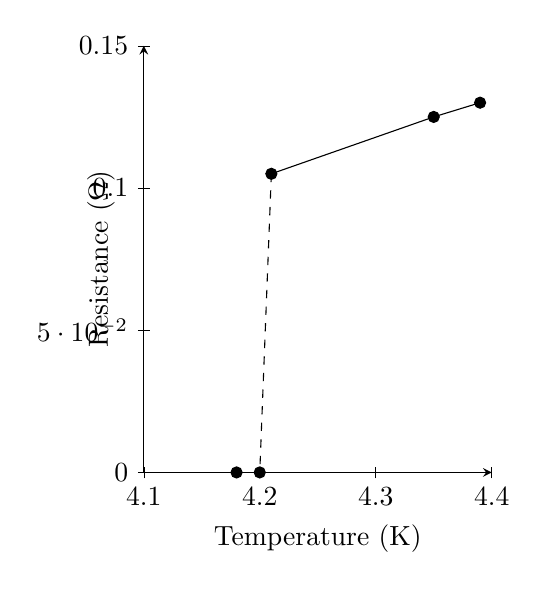
\begin{tikzpicture}
	\begin{axis}[
			width=6cm,
			height=7cm,
			xlabel={Temperature (K)},
			ylabel={Resistance ($\Omega$)},
			y label style = {at={(axis description cs:-0.055555,.5)},anchor=south},
			xmin=4.1,
			xmax=4.4,
			ymin=0,
			ymax=0.15,
			axis lines=left,
			tick style={black},
			no markers,
			samples=5
		]
		% Data points
		\addplot[only marks, mark=*] coordinates {
				(4.18, 0.000009)
				(4.20, 0.00001)
				(4.21, 0.105)
				(4.35, 0.125)
				(4.39, 0.130)
			};

		% Interpolation line
		\addplot[mark=*] coordinates {
				(4.21, 0.105)
				(4.35, 0.125)
				(4.39, 0.130)
			};

		\addplot[dashed, mark=*] coordinates {
				(4.21, 0.105)
				(4.20, 0.00001)
			};
	\end{axis}
\end{tikzpicture}

	\caption{The resistance of Mercury in function of the temperature of the sample, taken from~\cite{tsukerman2020compendium}}
	\label{img:mercury-resistance}
\end{figure}

Later studies discovered that many materials, pure and alloy, could be brought to the
superconducting state as long as three conditions were met:
\begin{itemize}
	\item The temperature of the sample didn't exceed the critical temperature $\tc$,
	\item The current density flowing in the sample didn't exceed the critical current
	      density $\jc$,
	\item The magnetic field acting on the material didn't exceed the critical magnetic field $\bc$.
\end{itemize}

When a material reaches the superconducting state it exhibits perfect diamagnetism, which means that
the material is able to perfectly expel the magnetic field lines from its volume (a simple experimental proof of this effect
is given by the magnetic levitation effect). This capacity was first observed by
Meissner and Ochsenfeld in 1933~\cite{meissner1933}. In 1935 the London's equations tried to explain
exotic behavior of different superconductor alloys which, in some situations, do not exhibit a perfectly diamagnetic behavior and allow the
penetration of external magnetic field lines down to a certain depth, known as the London's
penetration depth~\cite{london1935}. This property of superconductors was actually already theorized by Dutch
physicist Geertruida de Haas-Lorentz, who published some preliminary research in~\cite{fokker1925physica}.

The diamagnetic properties of superconductors depend heavily on the material microscopic properties. Two different Types of superconductors have been
identified and studied~\footnote{
	In general superconductor behavior can be explained through
	Ginzburg-Landau theory~\cite{Cyrot1973} but very recent research has proven that not every
	superconductor can be described using the \textsc{gl} equation as shown
	in~\cite{diamantini2023typeiiisuperconductivity}, this lead to the preliminary definition of
	a new type of superconductor, but, due to how recent the research is, it seems that, at the
	time of writing, nobody other than Diamantini published in the field of Type III superconductivity.
}, in the following I will provide a brief description of each.

\section{Type I superconductors}
\label{sec:type1}
\Cref{fig:type1-transition}, plots magnetization, measuring the amount of induced or
permanent magnetic dipole moment of a magnet per unit volume~\cite{polarization-magnetization},
against external magnetic field $B$, applied on the sample. Once the magnetic field reaches $\bc$ the
magnetization of Type I superconductors drops to $0$.
\begin{figure}[!ht]
	\centering
	\begin{tikzpicture}
	% Axes
	\draw[->] (0,0) -- (5,0) node[right] {Applied Magnetic Fields, $B$};
	\draw[->] (0,0) -- (0,4) node[above] {Magnetization, $-M$};

	% Critical field B_c
	\node[below] at (3,0) {$B_c$};

	% Plot lines
	\draw[thick] (0,0) -- (3,3) -- (3,0);
\end{tikzpicture}

	\caption{Magnetization of a superconducting coil plotted against the external magnetic
		field, reproduction of the original plot taken
		from~\cite{slimani2022superconducting}} \label{fig:type1-transition}
\end{figure}
As long as the applied magnetic field is less than $\bc$, Type I superconductors exhibit perfect
diamagnetism, but once the material undergoes a transition to the normal-conducting
state (which will be referred to as \emph{quench} from now on) the magnetic dipole exerted by the
superconductor falls to zero (or a negligible value) allowing magnetic field penetration and making
such materials unsuitable for environments where a high magnetic field is required, such as fusion
reactors or particle physics experiments.

\section{Type II superconductors}
\label{sec:type2}
Type II superconductors, in most cases, are metal alloys. The characteristical impurity gives Type II superconductors an edge
over Type I, for high-field applications, due to the graceful degradation of magnetization with the increase in applied magnetic
field. A plot similar to \Cref{fig:type1-transition} can be seen in \Cref{fig:type2-transition}.
\begin{figure}[!ht]
	\centering
	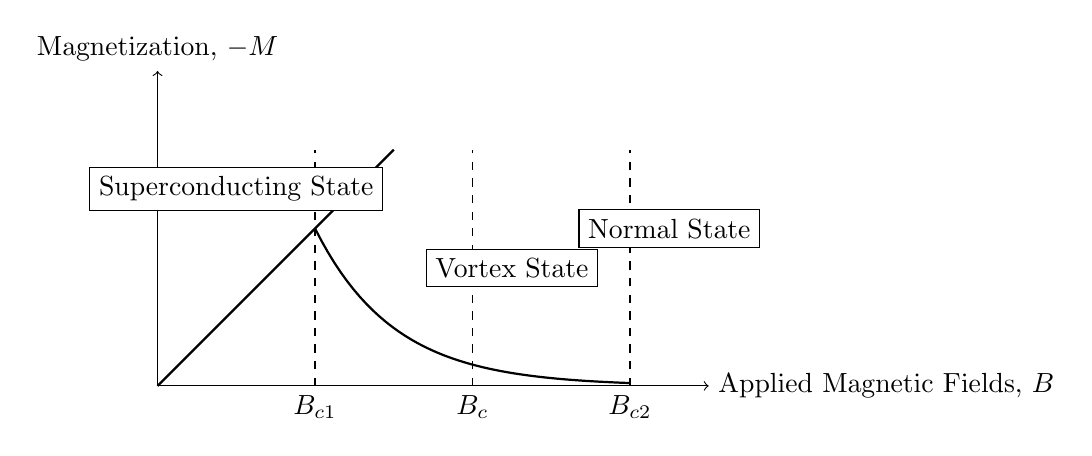
\begin{tikzpicture}
	% Axes
	\draw[->] (0,0) -- (7,0) node[right] {Applied Magnetic Fields, $B$};
	\draw[->] (0,0) -- (0,4) node[above] {Magnetization, $-M$};

	% Critical field labels
	\node[below] at (2,0) {$B_{c1}$};
	\node[below] at (4,0) {$B_c$};
	\node[below] at (6,0) {$B_{c2}$};

	% Dashed lines for critical fields
	\draw[dashed] (2,0) -- (2,3);
	\draw[dashed] (4,0) -- (4,3);
	\draw[dashed] (6,0) -- (6,3);

	% Magnetization curve
	\draw[thick] (0,0) -- (3,3);
	\draw[thick, domain=2:6, samples=50] plot (\x, {2*exp(-(\x-2))});

	% State labels with rectangles
	\node[draw, fill=white] at (1,2.5) {Superconducting State};
	\node[draw, fill=white] at (4.5,1.5) {Vortex State};
	\node[draw, fill=white] at (6.5,2) {Normal State};

\end{tikzpicture}

	\caption{Magnetization of a type II superconducting coil plotted against the external
		magnetic field, reproduction of the original plot taken from~\cite{slimani2022superconducting}}
	\label{fig:type2-transition}
\end{figure}

Type II superconductors, while the applied magnetic field is less than $B_{C1}$, have the same
diamagnetic properties of Type I superconductors. Once the applied magnetic field surpasses the
$B_{C1}$ threshold, instead of having a very sharp transition from the superconducting state to
the normal-conducting state, these materials remain in an intermediate state referred to as the \emph{vortex} or \emph{hybrid state}.

In the vortex state the external magnetic field is partially penetrating in the volume of the superconductor, but the
flux lines are constrained in particular columns, pinned within the lattice of the
superconductor, called \emph{Abrikosov vortices} or \emph{fluxons}~\cite{abrikosov-vortices}.
A vortex is a closed-loop supercurrent surrounding the magnetic field lines that
penetrate the material. Supercurrents, also known as persistent currents, are extremely stable and as long as the material remains in the
superconducting state they don't decay~\cite{fujita-theory-HTS, file1963}, as a matter of fact, as long as the
fluxons are pinned in place, the material remains locally superconductive. Vortices are usually anchored to imperfections in the material, that is why alloys and anisotropic materials are usually Type II superconductors.

\begin{figure}[!ht]
	\centering
	\begin{tikzpicture}

	\pgfmathsetmacro{\z}{3}

	\foreach \x in {2, 4.5, 7} {
			\node (vortex) [cylinder, shape border rotate=90, draw,minimum height=3cm,
				minimum width=0.5cm] at (\x, 2, \z){};
			\draw[thick, ->] (\x,2,\z) -- (\x,4,\z) node[right] {};

			\foreach \y in {1, 2, 3} {
					\begin{scope}[shift={(\x,\y,\z)}]  % Shift the ellipse to (2,2) in XY plane
						\draw[thick, postaction={decorate}, decoration={markings, mark=at position 0.6 with {\arrow{>}}}] (0,0) ellipse (0.5 and 0.2);
					\end{scope}
				}
		}

	\draw[thick, ->] (10, 1, 3) -- (10, 4, 3) node[right] {$\mathbf{B}$};

	% Vertices of the cube
	\coordinate (A) at (0,0,0);
	\coordinate (B) at (8,0,0);
	\coordinate (C) at (8,3,0);
	\coordinate (D) at (0,3,0);
	\coordinate (E) at (0,0,3);
	\coordinate (F) at (8,0,3);
	\coordinate (G) at (8,3,3);
	\coordinate (H) at (0,3,3);

	% Draw the edges of the cube
	\draw
	(B) -- (C)
	(C) -- (D);
	\draw
	(E) -- (F) -- (G) -- (H) -- cycle;  % Top face
	\draw[dashed]
	(A) -- (B)
	(A) -- (E)
	(A) -- (D);
	\draw
	(B) -- (F)
	(C) -- (G)
	(D) -- (H);
\end{tikzpicture}

	\caption{Schematization of a lattice of vortices, each surrounded by a
		supercurrent.}
	\label{fig:abrikosov-lattice}
\end{figure}

\Cref{fig:abrikosov-lattice} is a simplified schema of the fluxon lattice, as we can see each
supercurrent (the rings in figure), surrounds a \emph{quantized} amount of magnetic flux
$\vec{\varphi}_0$. If a density of current $\vec{J}$ is flowing through a superconductor it will
generate a Lorentz force $\vec{F}_L = \vec{J} \times \vec{\varphi}_0$, capable of inducing vortex
movement, if the $\vec{J}$ is high enough. If the vortices begin to move under this influence, and
the generated electric field $\vec{E}$ is parallel to the direction of the current, then the motion
produces a dissipation of power due to Joule effect.

This was a simplified description of the effects of vortex movement in a superconductor lattice, not
taking into account many factors like flux pinning and quantum effects, for a more thorough
dissertation refer to~\cite{huebener2019}.

\section{Quench}
As was said in a previous section, whenever a superconductor exhibits a local transition to the
normal-conducting state, therefore developing a finite electrical resistance, an exponentially
growing cascade effect might occur. The transition might be particularly destructive if left
unchecked, because the presence of electrical resistance in a superconductor carrying a very high
current density might cause local joule heating power distribution that can lead to localized
material damage. That is why, normally, in the field of accelerator physics, superconducting magnets
are accompanied by \textsc{qps} (Quench Protection Systems), which interrupt power delivery whenever
one of the superconducting coils show an irreversible transition as a local rising of resistive
voltage in the electrical powering circuit.

\chapter{Machine learning: an overview}
\label{chp:ml}
This chapter is dedicated to the theoretical exploration of some of the most important concepts in
machine learning alongside the various models that have been used in the project. We will begin with
a concise explanation of the more basic concepts linked to machine learning, then we will move to a
theoretical overview of the supervised models used for the project, followed by a brief introduction to
unsupervised machine learning models.

\section{Supervised machine learning}
\label{sec:sml}
Due to the popularization of artificial intelligence in recent times, it's very important to establish the field to avoid the risk of
incurring in misunderstandings. \emph{Machine learning} is a subset of artificial
intelligence, and is a technique that allows us to solve a problem without the need to actually invent an
algorithm to solve it (as long as there is enough data). There are many different problems that
either lack an algorithmic solution or have an inefficient one; in such cases, machine learning is
an alternative worth exploring. The tradeoff of using machine learning instead of 'classic'
problem-solving techniques is that the solution is built using heuristic methods,
therefore is not \emph{correct} for the problem \cite{Rebala2019}.

\medskip

A supervised machine learning model is a model $\model$ capable of learning a mapping between the
input space $\ins$ and the output space $\outs$ and then apply this mapping to unseen
data to predict the output \cite{Cunningham2008}.

\smallskip

Given a problem $\problem$, a specific instance of $\problem$, $\problem_i$, is characterized by a pair
$(\vec{x}_i, y_i)$ where $\vec{x}_i \in \ins$ are vectors taken from an input space $\ins$, usually
highly dimensional, and $y_i \in \outs$ are the expected solutions, which can be scalar or
vector\footnote{Outcomes will be considered scalars for the rest of this thesis unless explicitly
	stated}. The single components of every input vector, $\vec{x}_i$, are called
\emph{features}, and are values (numerical or other) representing a particular aspect of the domain.

A \emph{dataset} is a set containing $m$ problem instances $\dset$, and
a supervised machine learning model $\model$, trained on $D$, can be used to predict the outcome,
$\hat{y}$, of any instance of the problem $\problem_i$. Note that a machine learning model is the result of a
statistical process, therefore is susceptible to change unless the randomicity is kept under control.
On a practical level we can make sure that, for reproducibility purposes, the random number
generators associated to the various libraries are set to a definite value.

\medskip

To clarify the concepts just introduced, let us consider the following mock-problem: 'Is it going to rain
tomorrow?'. The dataset $D$ contains $365$ instances of the problem, one per day, for a year. The
input vector for every problem is a set of atmospheric measurements (e.g., temperature, atmospheric
pressure, exposure, humidity, \ldots), each measurement a different feature of the dataset. The
output of every instance $\problem_i$ is a flag answering the question 'did it rain on day $i$?'
with a $1$, for True, and a $0$, for False.

Due to the high grade of complexity of the problem solved in this thesis, future concepts will be clarified
using this exact mock-problem or its variations.

\medskip

In general, a machine learning problem can be defined as the process of finding the mapping that
relates the input space $\ins$ to the output space $\outs$ by abstracting patterns from
a training set. Conventionally, the output space can be interpreted differently based on
the problem:
\begin{itemize}
	\item $\outs = \{-1, 1\}$, for \emph{binary classification} problems, which are usually
	      associated with pattern recognition tasks, a very easy example of binary classification is our mock-problem.
	\item $\outs = \{a_1,\ldots, a_m\}$, for \emph{multi-class classification} problems, in
	      which an element can be part of one of the classes in a certain set, a classic
	      example is the character recognition problem, in which a certain character given in input can belong to one of 10 different classes (the numbers from 0 to 9) \cite{pal2010handwritten}.
	\item $\outs = \mathbb{R}$, for \emph{regression problems}, which are usually associated
	      with function approximation tasks, an example of regression problem
	      is: 'Based on the current amount of wins for Oklahoma City Thunder\footnote{An
		      amazing \textsc{nba} team}, predict the team's win rate at the end of the season'.
\end{itemize}

Most machine learning models have to go through the same steps, described here below
\begin{itemize}
	\item \emph{Model selection}: if we consider an instance of a decision tree (introduced in
	      \Cref{sec:dt}), the model can be described through a set of characteristics (e.g.,
	      number of nodes, depth, splitting method, \ldots), all of these are known as
	      \emph{hyperparameters}. An important step of solving a machine learning problem is
	      doing an exploration, even if not thorough, due to the exponential complexity of the
	      task, of the hyperparameter space, to find the best possible combination for the
	      problem.
	\item \emph{Model training}: during the training procedure, the instance of the model abstracts
	      patterns from a sample of the dataset, which we will call \emph{training set} $T$.
	\item \emph{Model testing}: during the testing procedure the model performance is tested on a
	      part of the dataset, which we will call \emph{test set} $G$ (standing for
	      \emph{generalization}). This set is used to understand whether the performance found for model
	      $\model$ is a statistical anomaly (therefore depending on the points
	      chosen to build $T$) or extends also to unseen data.
\end{itemize}

There are many different approaches to splitting a dataset $D$ into a series of separate parts
for the various tasks involved in the machine learning problem resolution (e.g., model training,
model testing, model selection, \ldots). In the following I will describe two non-trivial aspects of
the basic procedure to split a dataset $D$ into a training dataset $T$ and a testing dataset $G$ and a
more complex splitting procedure will be introduced at a later time.

\medskip

As a first non-trivial aspect of the splitting procedure is that, depending on the problem, making
sure that the distribution of training dataset $T$ and testing dataset $G$ is the same as the
original dataset distribution is important. To understand why, let's think about a dataset
$\dset$ in which every $\mathbf{x}_i \in \ins$ is a vector of features describing a patient's
conditions (e.g., age, sex, body temperature, blood saturation, \ldots) and every $y_i \in \outs$ is
a string indicating which illness was diagnosed (e.g., flu, pneumonia, \textsc{covid}, ...). Supposing we want to find a
model $\model$ capable of doing a diagnosis effectively: we need to make sure that the least
represented illnesses (which are usually the more dangerous ones) are well represented in both $T$
and $G$. If this splitting process was not done correctly we might end up with a model $\model$ that
can reliably recognize a common flu but can't correctly identify serious illnesses like pneumonia.

\medskip

The second non-trivial aspect of the splitting procedure is that it's always necessary to make sure
that the operation is carried out independently for each dataset, this means that data that is in the
training set cannot be in the testing set, and vice versa. If this were not to be true then we would
have a data leak from one set to the other.

\smallskip

Whenever a data leak is identified from the training set $T$ to the testing set $G$, some points
that were used to train $\model$ are used once more to test its performance, which leads to a higher
performance metric, relaying higher and unjustifed confidence in the model performance.

\medskip

To close this section about supervised learning, we will be introduced to two issues specific to
supervised learning models. Whenever we work in the field of supervised learning it's important to be aware of two classic issues: \emph{overfitting} and \emph{underfitting}.

\smallskip

Given the generic machine learning problem $\problem$ and a dataset $\dset$, the model $\model$ that
solves $\problem$, is said to be overfitting when the training performance is acceptable, but the
testing performance is unacceptably bad; this means that the mapping found by $\model$ to link $\ins$
and $\outs$ is too closely related to the specific data chosen to do the training, therefore
unable to generalize effectively. In other
words, $\model$ is overfitting whenever, instead of abstracting some general patterns in the
data, it actually learns some peculiarities of the specific training dataset $T$ \cite{ZhouZhi-Hua2021ML}
which are not found later in the testing dataset $G$.

\smallskip

An 'orthogonal' problem to overfitting is the issue of \emph{underfitting}, which is usually caused
by a model not being powerful enough to abstract information from a certain dataset. Whenever a
machine learning model is underfitted for a problem $\problem$, the performance metrics obtained
during training and testing are unacceptably bad, independently of the train and test set
utilized.

\medskip

The problem that this thesis aims to solve takes full advantage of supervised models, since the data at our
disposal has already been analyzed and labelled in previous works \cite{mariotto2022}\cite{mariotto2022-generic}.

\medskip

In the following we will be discussing, on a theoretical level, the various supervised models deployed
to solve the problem.

\section{Decision Trees}
\label{sec:dt}
This section is a theoretical introduction to decision trees, the implementation we used for the
model is the \emph{DecisionTreeClassifier} class contained in scikit-learn.

\medskip

A decision tree is a machine learning model based on a tree structure, an example of such a
structure can be seen in \Cref{fig:simple-dt}. Each internal node contains a condition that needs to
be evaluated on one or more features (e.g.,  the root of \Cref{fig:simple-dt} requires us to check
whether the humidity feature of the input is $\geq 80\%$), if the result of the evaluation is true
the computation proceeds with the left child, otherwise the right path will be taken. Once a leaf is
reached, the class associated to the point is identified. If we consider again \Cref{fig:simple-dt}
we could say that if the humidity of the input is $\geq 80\%$ and the temperature is $\geq 10C$ then
the inputs will be classified as 'rain'.

Any path leading from root to leaf is known as a \emph{decision path}. It's evident that such structures have a very high degree of explainability and that is why usually they are the first model chosen to solve a machine learning problem.

\medskip

Two are the theoretical concepts I wish to cover in this section: indices and node split
computation, avoiding overfitting through pre- and post- pruning.
\begin{figure}
	\centering
	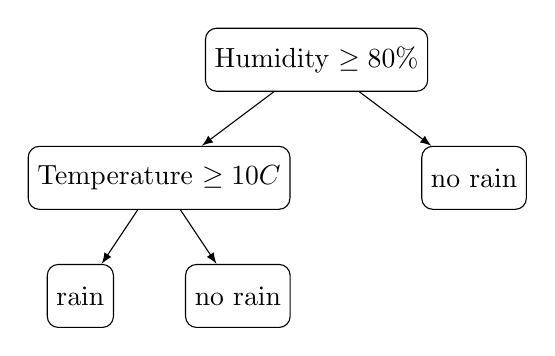
\begin{tikzpicture}[
			% Define styles for nodes
			level 1/.style={sibling distance=40mm},
			level 2/.style={sibling distance=20mm},
			level 3/.style={sibling distance=10mm},
			every node/.style={draw, rectangle, rounded corners, align=center, minimum size=8mm},
			edge from parent/.style={draw, -latex}
		]

		% Root node
		\node {Humidity $\geq 80\%$}
		% First level
		child {node {Temperature $\geq 10C$}
				% Second level
				child {node {rain}}
				child {node {no rain}}
			}
		child {node {no rain}};
	\end{tikzpicture}
	\caption{A very simple example of decision tree built on the mock problem}
	\label{fig:simple-dt}
\end{figure}
\subsection{Indices and node split computation}
In \Cref{fig:simple-dt} a simple structure for a decision tree was shown, an excellent question in
its regard could be: 'Why this structure and not another one?'. Other than it being a simple example
nothing is really preventing us from describing the 'rain' event based on different threshold values
or different feature sets altogether.
\begin{figure}
	\centering
	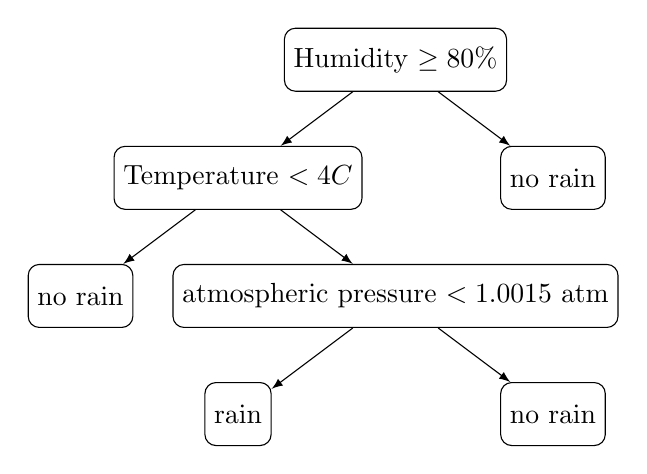
\begin{tikzpicture}[
			% Define styles for nodes
			level 1/.style={sibling distance=40mm},
			level 2/.style={sibling distance=40mm},
			level 3/.style={sibling distance=40mm},
			every node/.style={draw, rectangle, rounded corners, align=center, minimum size=8mm},
			edge from parent/.style={draw, -latex}
		]

		% Root node
		\node {Humidity $\geq 80\%$}
		% First level
		child {node {Temperature $< 4C$}
				% Second level
				child {node {no rain}}
				child {node {atmospheric pressure $< 1.0015$ atm}
						child{node {rain}}
						child{node {no rain}}
					}
			}
		child {node {no rain}};
	\end{tikzpicture}
	\caption{Another decision tree built on the mock-problem and alternative to
		\Cref{fig:simple-dt}}
	\label{fig:simple-dt-alt}
\end{figure}
The mock tree shown in \Cref{fig:simple-dt-alt} is a different tree compared to the one shown in
\Cref{fig:simple-dt} and yet they solve the same problem by characterizing it differently.
\Cref{algo:decision-tree} shows how the decision tree is built, line $9$ states that the best
splitting feature needs to be selected with every iteration, this choice is taken based on a
\emph{purity} index applied to nodes.

\begin{algorithm}
	\caption{The decision tree base algorithm taken from
		\cite{ZhouZhi-Hua2021ML}}\label{algo:decision-tree}
	\begin{algorithmic}[1]
		\Require Training set $\dset$ and Feature set $A = \{a_1, \ldots,
			a_d\}$.
		\Ensure A decision tree
		\Function{TreeGenerate}{$D$, $A$}
		\State Generate node $i$;
		\If{All samples in $D$ belong to the same class $C$}
		\State Mark node $i$ as a class $C$ leaf node; \textbf{return node $i$}
		\EndIf
		\If{$A = \emptyset$ \textsc{or} all samples in $D$ take the same
			value on $A$}
		\State Mark node $i$ as a leaf node, its class label is
		the majority in $D$;
		\State \textbf{return node $i$}
		\EndIf
		\State Select the optimal splitting feature $a_*$ from $A$;
		\For{each value $a_*^v$ on $a_*$}
		\State Generate a branch for node $i$;
		\State Let $D_v$ be the subset of samples taking value $a_*^v$ on $a_*$;
		\If{$D_v$ is empty}
		\State Mark this child node as a leaf node;
		\State label t with the majority class of $D$;
		\textbf{return node $i$}
		\Else
		\State use \textproc{TreeGenerate}$(D_v, A \setminus \{a_*\})$ as the child node.
		\EndIf
		\EndFor
		\EndFunction
	\end{algorithmic}
\end{algorithm}

\medskip

The purity of a node defines how heterogeneous are the samples associated to it. Intuitively, in the
context of our mock-problem: if the distribution of samples arriving to a node $i$ is $15$ labelled
$1$, and $1$ labelled $0$, then the purity of the node is going to be very high.

A split is going to be performed on feature $a$ only if the resulting purity increase is the best
possible. There are many different indices used to compute purity, in the following I will be
considering only the ones important for the model selection process that will be introduced in
a future chapter: \emph{Entropy} and \emph{Gini index}.

\subsubsection{Entropy}
There are many different ways of defining information entropy, a more general definition, compared
to the one found in \cite{ZhouZhi-Hua2021ML}, is found in \cite{gray2011entropy}. Let's consider a
random variable $f$ built on the alphabet $B = \{b_1, \ldots, b_{|B|}\}$ we can define the
partition $\mathcal{Q} = \{Q_i: i = 1, \ldots, |B|\}$ where $Q_i = \{\omega: f(\omega) = b_i\} = f^{-1}(b_i)$ therefore $\mathcal{Q}$ is a partition of the bigger
probability space $\Omega$, every partition is chosen based on the outcome of the
measurement of the random variable $f$. In the case of a discrete random variable we can define the
information entropy as shown in \Cref{eq:information-entropy}
\begin{equation}
	\label{eq:information-entropy}
	H_p(\mathcal{Q}) = - \sum_{i = 1}^{|B|}{P(Q_i)\log{P(Q_i)}}
\end{equation}
this definition of entropy can be easily extended to the dataset case since:
\begin{itemize}
	\item The partition set $\mathcal{Q}$ can be mapped to the dataset $D$,
	\item Every partition $Q_i$ can be mapped to the single class of the machine learning
	      problem that is being considered,
	\item The alphabet $B$ can be mapped to the set of possible outcomes of the machine learning
	      problem.
\end{itemize}
Therefore, we can rewrite \Cref{eq:information-entropy} as:
\begin{equation}
	H_p(D) = - \sum_{k = 1}^{|\outs|}p_k \log{p_k}
\end{equation}
$p_k$ denotes the proportion of the $k$-th class inside dataset $D$.

If we consider the binary classification problem ('true' or 'false' response), whenever a splitting procedure
is done on a node in the tree, the split is computed on every feature based on the possible
values of the feature itself (only for discrete features), if we consider our mock-problem, a split could be computed on a
feature called  'status of the sky' which can have one of two values $\{\text{overcast},
	\text{clear}\}$ the new node could be built in two different ways and
the class distribution for each is different, having different levels of purity based
on how well the data is partitioned between the classes 'rain' and 'no rain'.

\smallskip

To choose which of the two nodes to take in our mock-problem using the entropy measure we need to
introduce the concept of \emph{information gain}, which is expressed as follows:
\begin{equation}
	\label{eq:information-gain}
	\textsc{Gain}(D, a) = H_p(D) - \sum_{v = 1}^V\frac{|D^v|}{|D|}H_p(D^v)
\end{equation}
The concept expressed by information gain in \Cref{eq:information-gain} is that the amount of
information gained by doing a split of dataset $D$ on feature $a$ is given by the entropy of dataset
$D$ at the moment of the split from which we remove the entropy of the dataset resulting from the
split of feature $a$ at every value $v$ scaled by the ratio between the cardinality of the new dataset to
the cardinality of the original dataset.

\smallskip

The feature used to perform the actual splitting is going to be the one with the highest possible
information gain. It's very important to notice that information gain is an index biased towards
features that have many different values (and therefore $|D^v|$ is small). In the case of our mock
problem, if we consider 'status of the sky' and we compare it to another feature containing many
different splitting values for example 'cloud color' which might assume the following values
$\{\text{white}, \text{light grey}, \text{grey}, \text{black}, \text{pink}, \text{orange},
	\text{red}\}$ it's clear that the $|D^v|/|D|$ is going to be lower for each of them, therefore
leading to a lower entropy decrease and a higher information gain.

\medskip

The alternative to using information gain is to use the \emph{gain ratio}
\begin{equation}
	\label{eq:gain-ratio}
	\textsc{GainRatio}(D, a) = \frac{\textsc{Gain}(D, a)}{\textsc{iv}(a)}
\end{equation}
the \textsc{iv} function in \Cref{eq:gain-ratio} is the \emph{intrinsic value} of feature $a$ and
can be computed as shown in \Cref{eq:intrinsic-value}.
\begin{equation}
	\label{eq:intrinsic-value}
	\textsc{iv}(a) = - \sum_{v = 1}^V\frac{|D^v|}{|D|} \log{\frac{|D^v|}{|D|}}
\end{equation}
Due to how intrinsic value is defined the gain ratio corrects the bias of the information gain towards features
with a higher number of values but is biased towards features with a lower amount of variables
\cite{ZhouZhi-Hua2021ML}.

In the actual implementation of the decision tree provided by scikit-learn an optimized version of
the \textsc{cart} algorithm is used, which  is similar to the \textsc{c4.5} algorithm proposed by Quinlan in
\cite{quinlan2014c4}.

\subsubsection{Gini index}
The original \textsc{cart} algorithm conceptualized by Breiman et al. in 1984
\cite{breiman1984classification} used Gini index to compute the best splitting feature for every
node. The Gini value of a dataset can be computed as shown in \Cref{eq:gini-value}
\begin{equation}
	\label{eq:gini-value}
	\textsc{Gini}(D) = \sum_{k = 1}^{|\outs|}\sum_{k' \neq k} p_kp_{k'} = 1 - \sum_{k =
		1}^{|\outs|}p_k^2
\end{equation}
As explained in \cite{ZhouZhi-Hua2021ML}, \Cref{eq:gini-value} can be interpreted as the
likelihood of taking samples from two different classes by drawing them randomly from the
dataset, the lower the $\textsc{Gini}(D)$, the higher the purity of a node. Gini index can be
computed as the weighted sum of all the Gini values for the dataset after the split, as shown in
\Cref{eq:gini-index}.
\begin{equation}
	\label{eq:gini-index}
	\textsc{GiniIdx}(D) = \sum_{v = 1}^V\frac{|D^v|}{|D|} \textsc{Gini}(D^v)
\end{equation}

The best splitting feature is going to be the one with the smallest Gini index overall.

\subsection{Avoiding overfitting through pre- and post- pruning}
As was argued in the previous section decision trees have an extremely simple structure and they
allow us to interpret the obtained results giving us an idea of how the machine is able to classify
our points.

Overfitting is probably the biggest drawback of decision trees, as shown in
\cite{overfitting-dt-erblin}, since the model tries to partition the space based on the purity of
the nodes it's important to make sure that the rules utilized to do partitioning do not become too
specific. There are two techniques explained in the literature that can be used to prevent the model
from overfitting: Pre-pruning and post-pruning.

\medskip

Pre-pruning consists in a set of rules that force the algorithm to an early stop whenever a series
of conditions allow it. In the literature pre-pruning is sometimes associated only to a technique
that stops the splitting procedure whenever the impurity decrease (or the purity increase) doesn't
justify the split in the first place \cite{ZhouZhi-Hua2021ML}; I find myself more in line with
the general definitions given in \cite{bramer2007principles}\cite{fisher1996learning}, which
state that pre-pruning is a group of techniques meant to keep the size of the tree in check.

The specific pre-pruning conditions that can be checked using the DecisionTreeClassifier class provided by
scikit-learn are the following:
\begin{itemize}
	\item The tree \emph{depth}, avoiding a complex tree structure by cutting the depth is
	      probably one of the easiest forms of pre-pruning.
	\item The \emph{impurity decrease} stops nodes from splitting when the decrease in impurity
	      of the children is not higher than a certain threshold, if the threshold is too high
	      then the tree will probably underperform, if it's too low then the tree is going to
	      overfit.
	\item The \emph{number of elements to split} is basically a check that can be done on the
	      number of points inside a node. Not splitting when the number of points
	      contained in a node is too little is ax excellent way of avoiding overfitting.
\end{itemize}

\medskip

Post-pruning is the alternative to pre-pruning, the essential difference between the two is that
post-pruning is done after the tree has been fully constructed, therefore, in the a posteriori phase
a series of branches will be chosen to be pruned based on the impurity decrease that they provide.
There are different post-pruning techniques that can be implemented, scikit-learn is working with
Cost Complexity Pruning (\textsc{ccp}), introduced in \cite{breiman1984classification}.

\section{Ensemble learning}
\label{sec:el}
In the previous chapter I introduced decision trees, and we have talked at length about their
strength and weaknesses, providing some instruments to counter their shortcomings. Sometimes,
despite our efforts, the decision tree model is simply not enough for the task at hand, if we don't
want to give up the high explainability of tree models, in favor of higher performance, we can think
of creating an ensemble.

An ensemble is constructed by grouping weaker learners, which produces two main effects (to
clarify the concepts we will consider a basketball roster):
\begin{itemize}
	\item Different learners are able to grasp different sides of the problem, which would be
		either impossible or complicated for single models, if we consider our example, each
		player covers different positions which do not fit the other players (this doesn't
		mean that key players or superstars cannot play in other positions due to their
		performance).
	\item Using a group of models alleviates the shortcomings of the weaker links in the chain,
		if we consider our example, the weaker players, and lesser role players, can stay on the bench while the
		main rotation is playing, but can still contribute with some quality minutes when
		the main rotation is facing a difficulty.
\end{itemize}

Following the analysis done in \cite{ZhouZhi-Hua2021ML}, I will now prove that the error rate of a
binary classifier based on an ensemble of models falls to zero exponentially with the number of individuals
used.

Let's suppose that the error rate of each model in the ensemble is $\epsilon$, the ground truth
function is $f$ and the single learner is $h_i$, then we can express the probability of the learner
making a wrong prediction on $\vec{x} \in \ins$ as shown in \Cref{eq:error-rate}.
\begin{equation}
	\label{eq:error-rate}
	P(l_i(\vec{x}) \neq f(\vec{x})) = \epsilon
\end{equation}
Assuming that the prediction is $y \in \{-1, +1\}$, let's consider an ensemble in containing $T$
base learners, independent of each other, the ensemble will aggregate the predictions by using a
simple majority algorithm (\Cref{eq:ensemble-aggregation}).
\begin{equation}
	\label{eq:ensemble-aggregation}
	F(\vec{x}) = sign\left(\sum_{i = 1}^{T}l_i(\vec{x})\right)
\end{equation}
Since the probability of a base learner of being correct is $1 - \epsilon$, then the ensemble
correctly classifies a sample only if more than half of the learners correctly identify the sample.
This is expressed by \Cref{eq:succ-probability}.
\begin{equation}
	\label{eq:succ-probability}
	\begin{aligned}
		Pr(\text{success}) & = Pr\left(\text{at least } \left\lceil{\frac{T}{2}}\right\rceil \text{ correctly identify
		the sample}\right)
		\\
			   & = \sum_{k = \lceil{T / 2}\rceil}^T \binom{T}{k} (1 - \epsilon)^k
			   \epsilon^{T - k}
	\end{aligned}
\end{equation}
Since we are interested in finding a bound for ensemble error rate we are interested in the
complement of $Pr(\text{success})$, which is $Pr(\text{insuccess}) = Pr(F(\vec{x}) \neq
f(\vec{x}))$. The ensemble misclassifies a sample only if the number of learners that can correctly classify the
model is less than half, therefore $Pr(\text{insuccess})$ can be defined, starting from
\Cref{eq:succ-probability} as shown in \Cref{eq:insucc-probability}.
\begin{equation}
	\label{eq:insucc-probability}
	Pr(\text{insuccess}) = Pr(F(\vec{x}) \neq f(\vec{x})) = \sum_{k = 0}^{\lfloor{T / 2}\rfloor} \binom{T}{k} (1 - \epsilon)^k \epsilon^{T - k}
\end{equation}
Due to the independence assumption we can use Hoeffding's inequality on the sum of independent
random variables \cite{ZhouZhi-Hua2021ML}, result is an upper bound of the error rate.
\begin{equation}
	\label{eq:hoeffding}
	\sum_{k = 0}^{\lfloor T / 2 \rfloor}\binom{T}{k} (1 - \epsilon)^k\epsilon^{T - k} \leq
	exp\left(-\frac{1}{2}T(1 - 2\epsilon)^2\right)
\end{equation}
\Cref{eq:hoeffding} is telling us that the error rate of the ensemble falls exponentially with the
number of base learners $T$. This proof is based on the non-trivial assumption that the base
learners are independent of each other, which is something that doesn't apply in the practical
case, since the models are trained on the same dataset for the same problem $\problem$.

\medskip

Before doing a brief overview of the random forest model I will introduce Bagging, which is the
technique at the base of the random forest model.

\subsubsection{Bagging}

Bagging, introduced by Leo Breiman in \cite{Breiman1996}, is a method for generating multiple
version of a base predictor that are then aggregated in a single predictor, following
\cite{ZhouZhi-Hua2021ML} the algorithm can be easily outlined in \Cref{algo:bagging}.
\begin{algorithm}
	\caption{The bagging algorithm, taken from \cite{Bauer1999}}\label{algo:bagging}
	\begin{algorithmic}[1]
		\Require A training dataset $\dset$, a base learner $\mathcal{L}$, a certain number
		of training rounds $T$.
		\Ensure An ensemble model capable of aggregating predictions.
		\Function{Bagging}{$D$, $\mathcal{L}$, $T$}
		\For {$t = 1, \ldots, T$}
		\State $D_{bs}$ obtained by bootstrap sampling from $D$
		\State $h_t = \mathcal{L}(D_{bs})$ 
		\EndFor
		\State \textbf{return} $H(\vec{x}) = \argmin_{y \in \outs}\sum_{t : h_t(\vec{x}) =
		1} 1$
		\EndFunction
	\end{algorithmic}
\end{algorithm}
The algorithm can be described as follows: given a dataset $\dset$, we create a new dataset of size
$n$ ($D_{bs}$) in \Cref{algo:bagging} by randomly picking samples from $D$, if we repeat the
procedure $T$ times we obtain $T$ different datasets of size $n$, which are used to train different
base learners. Once the training is over, predictions can be done on inputs and the results of the
prediction can be aggregated using different techniques (e.g., majority voting, averaging, etc...).

\medskip

Since $D_{bs}$ is being built from $D$ without removal it's interesting to give an
estimate of the number of samples that are being actually used. Since the probability of being
picked is $1 / m$, and doesn't change with the iteration, the probability of not being picked is $1
- 1 / m$.

\smallskip

If we compute the limit of the probability for an extremely large dataset we get
\Cref{eq:bagging-limit}, telling us that we can expect that $36.8\%$ of the data remain unused.
\begin{equation}
	\label{eq:bagging-limit}
	\lim_{m \rightarrow \infty} \left(1 - \frac{1}{m}\right) = \frac{1}{e} \approx 0.368
\end{equation}
Since this data would be 'lost' on the estimator, we can implement a different version of the
train-test split seen in the beginning of the chapter: if we keep track of the data that ends in
$D_{bs}$, what remains can be put in $V_{bs}$, which is a validation set and can be used to understand how much
the single learner is able to generalize after training (this is one of the many approaches that can
be implemented based to avoid wasting data).

\subsubsection{Random Forests}

Random forests are an extension of the Bagging model that was just described, they were introduced
by Leo Breiman in \cite{Breiman2001}, while decision trees perform the splitting procedure for every
node by selecting the feature that yields the best impurity reduction, random forests pick the
feature that yields the best impurity decrease from a random subset of features of size $k$. The
value of $k$ controls how random is the splitting procedure, if $k = d$, where $d$ is the size of
the feature set, then the behavior of the random forest is the same as the decision tree introduced
in the last section, if $k = 1$, then the split feature is chosen randomly.

Despite the relative simplicity of the model random forests provide a high grade of performance,
accompanied by the same grade of explainability of decision trees (with the added complexity of
having to deal with more than one learner at the same time).

\section{SVM}
\label{sec:svm}
With this section we leave behind the tree-based models to talk about the benchmark model that we
chose for this thesis, an \textsc{svm} is a model with very high performance but low explainability,
in this chapter we will understand the theoretical foundations of this model. The main reference for
this chapter is going to be \cite{ZhouZhi-Hua2021ML}.

\medskip

Let's consider a binary classification problem on dataset $\dset$ with labels $y \in \{-1, +1\}$,
handling the classification task means to find a hyperplane that is able to divide the points in the
dataset 'reasonably well', since the number of such hyperplanes is infinite there are two
essential observations to be made:
\begin{enumerate}
	\item The space of the solutions cannot be checked thoroughly, therefore we will never know
	      if the hyperplane chosen is the best, or if there is another one that yields better
	      performance.
	\item The chosen hyperplane will be fitted on the dataset used for training,
	      but we can make sure that the generalization performance is good enough by making
	      sure that there is enough \emph{margin} between the separator and the 'hardest'
	      points in the dataset.
\end{enumerate}
The 'hardest' points are the ones closest to the hyperplane, referred to as \emph{support
	vectors}.

\medskip

We can express any hyperplane in space as a function (\Cref{eq:hyperplane}) of a normal vector
$\vec{w}$ controlling the direction of the hyperplane and a bias value $b$ controlling the distance
of the hyperplane from the origin.
\begin{equation}
	\label{eq:hyperplane}
	\vec{w}^\top\vec{x} + b = 0
\end{equation}
For any given point in space we can compute its distance from the hyperplane as shown in
\Cref{eq:hyperdistance}.
\begin{equation}
	\label{eq:hyperdistance}
	r = \frac{|\vec{w}^\top\vec{x} + b|}{||\vec{w}||}
\end{equation}
Let's suppose that the hyperplane can perfectly divide the points in the two classes, we can
describe it as shown in \Cref{eq:system}.
\begin{equation}
	\label{eq:system}
	\begin{cases}
		 & \vec{w}^\top\vec{x}_i + b > 0, \hspace{10pt} y_i = +1 \\
		 & \vec{w}^\top\vec{x}_i + b < 0, \hspace{10pt} y_i = -1
	\end{cases}
\end{equation}
\Cref{eq:svm-system} is valid for every point in the dataset, but we can give a stronger condition
which only works for the support vectors and is based on the distance defined in
\Cref{eq:hyperdistance}. This new system is shown in \Cref{eq:svm-system}.
\begin{equation}
	\label{eq:svm-system}
	\begin{cases}
		 & \vec{w}^\top\vec{x}_i + b \geq +1, \hspace{10pt} y_i = +1 \\
		 & \vec{w}^\top\vec{x}_i + b \leq -1, \hspace{10pt} y_i = -1
	\end{cases}
\end{equation}
The margin, defined in \Cref{eq:margin}, is the total distance between two support vectors belonging to different classes.
\begin{equation}
	\label{eq:margin}
	\gamma = \frac{2}{||\vec{w}||}
\end{equation}

\medskip

As was said in the beginning of this section, we want to find the best separating hyperplane,
therefore the hyperplane that has a reasonable distance from the hardest points in the training set
so that we can give some guarantees of the generalization performance. We can express this problem as a maximization problem:
we want to maximize the margin in \Cref{eq:margin} subject to the constraints of
\Cref{eq:svm-system}. Maximizing the margin means maximizing $||\vec{w}||^{-1}$ which is equivalent
to minimizing $||\vec{w}||^2$, taken for simplicity purposes. The problem, as is formulated in
\Cref{eq:primal}, is the primal form of \textsc{svm}.
\begin{equation}
	\label{eq:primal}
	\begin{aligned}
		\max_{\vec{w}, b}        & \frac{1}{2}||\vec{w}||^2                                            \\
		\text{s.t.}\hspace{10pt} & y_i(\vec{w}^\top\vec{x}_i + b) \geq 1 \hspace{10pt}i = 1, \ldots, m
	\end{aligned}
\end{equation}
This is a quadratic programming problem, there are libraries that provide solvers for the problem,
but there are other methods that allow us to compute a solution with a higher grade of efficiency.
We can introduce \emph{Lagrange multipliers} ($\alpha_i$ in \Cref{eq:lagrangian}), the resulting
Lagrangian is the one in \Cref{eq:lagrangian}.
\begin{equation}
	\label{eq:lagrangian}
	\lag(\vec{w}, b, \vec{\alpha}) = \frac{1}{2} ||\vec{w}||^2 + \sum_{i = 1}^{m}{\alpha_i (1 - y_i(\vec{w}^\top\vec{x}_i + b))}
\end{equation}
If we compute the partial derivatives of the Lagrangian with respect to $\vec{w}$ and the bias $b$
we obtain the two equations shown in \Cref{eq:pd-lagrangian}.
\begin{equation}
	\label{eq:pd-lagrangian}
	\begin{aligned}
		 & \frac{\partial{\lag}}{\partial{\vec{w}}} = \vec{w} - \sum_{i = 1}^m
		\alpha_iy_i\vec{x}_i                                                   \\
		 & \frac{\partial{\lag}}{\partial{b}} = \sum_{i = 1}^m \alpha_iy_i
	\end{aligned}
\end{equation}
By setting the partial derivatives to zero, and substituting the first in
\Cref{eq:lagrangian}, we can get rid of the normal vector dependency and the \emph{dual} problem can
be defined as a function of $\vec{\alpha}$ and the bias $b$. The dual problem is shown in \Cref{eq:dual}.
\begin{equation}
	\label{eq:dual}
	\begin{aligned}
		\max_{\vec{\alpha}}       & \left(\sum_{i = 1}^{m}{\alpha_i} - \frac{1}{2}\sum_{i =
		1}^{m}\sum_{j = 1}^{m}{\alpha_i\alpha_j y_i y_j \vec{x}_i^\top\vec{x}_j}\right)               \\
		\text{s.t.} \hspace{10pt} & \sum_{i = 1}^{m}{\alpha_i y_i} = 0 \hspace{10pt} i = 1, \ldots, m
	\end{aligned}
\end{equation}
The hyperplane that we are looking for can be modelled as shon in \Cref{eq:of}, the second
formulation is virtue of the substitution found for $\vec{w}$ in \Cref{eq:pd-lagrangian}.
\begin{equation}
	\label{eq:of}
	f(\vec{x}) = \vec{w}^\top\vec{x} + b = \sum_{i = 1}^m\alpha_iy_i\vec{x}_i\vec{x} + b
\end{equation}
Since \Cref{eq:primal} is an optimization problem with inequality constraints we
know from \cite{kkt1951} that solving it is equivalent to solving the dual problem based on the
Lagrangian defined in \Cref{eq:lagrangian} subject to the \textsc{kkt} constraints shown in
\Cref{eq:kkt-constraints}.
\begin{equation}
	\label{eq:kkt-constraints}
	\begin{cases}
		 & \alpha_i \geq 0                   \\
		 & y_if(\vec{x}_i) - 1 \geq 0        \\
		 & \alpha_i(y_if(\vec{x}_i) - 1) = 0
	\end{cases}
\end{equation}
For every point in the training set $(\vec{x}_i, y_i)$ only two scenarios are possible:
\begin{enumerate}
	\item Lagrange multiplier $\alpha_i = 0$, Therefore the point $(\vec{x}_i, y_i)$ is not
		influencing \Cref{eq:of}.
	\item If the Lagrange multiplier $\alpha_i > 0$ then the third constraint in
	      \Cref{eq:kkt-constraints} yields $y_if(\vec{x}_i) = 1$ which means that the point is
	      laying on the maximum margin hyperplanes, therefore it's a support vector.
\end{enumerate}
This reveals a very important detail: once the training is completed, the model can be entirely
described by using only support vectors, since they are the ones that yield a contribution in the
calculation of \Cref{eq:of}.

There are different techniques to solve the problem defined in \Cref{eq:dual}: one of the possibilities is to use quadratic
programming solvers, another possibility is to use the \textsc{smo} method; Proposed in
\cite{platt1998} and consisting of: an iterative resolution of the problem, by successive
identifications of local approximations of the Lagrange multipliers $\alpha_i$, while keeping all
other parameters frozen as constants.

\medskip

The method explained until now provides a solution to problem shown in \Cref{eq:primal} which is meant to
have perfect accuracy, meaning that no classification errors are accepted. This is a solution that
is neither advisable nor possible in most cases, due to the problem of linear separability addressed
in \Cref{sssec:kernel-functions}.

For this reason the \emph{soft margin} \textsc{svm} model was defined, such formulation of the solution
allows a relaxation of the constraints, therefore, a certain number of classification errors.
Since the number of errors needs to be minimized, we can rewrite the objective of \Cref{eq:primal} as
shown in \Cref{eq:sm-primal}.
\begin{equation}
	\label{eq:sm-primal}
	\min_{\vec{w}, b} \frac{1}{2}||\vec{w}||^2 + C\sum_{i = 1}^m \ell_{0 / 1}(y_i (\vec{w}^\top \vec{x}_i + b) - 1)
\end{equation}
In equation \Cref{eq:sm-primal} $C > 0$ is a regularization constant and $\ell_{0 / 1}$ is the $0/1$
loss. Solving directly the equation can be complicated, due to the poor mathematical properties of
the $0/1$ loss function, even if there are approximate methods to minimize it \cite{nguyen2013},
usually a convex loss function is used to replace it.

The soft margin \textsc{svm} is defined by substituting $0/1$ loss with hinge loss, a convex function for binary
classifiers defined as $\ell(y) = \max(0, 1 - ty)$ where $y$ is the raw output of the classifier and
$t$ is the label associated to the output, and then adding slack variables $\xi_i \geq 0$. The primal problem can be easily rewritten as shown in \Cref{eq:sm-primal-final}.
\begin{equation}
	\label{eq:sm-primal-final}
	\begin{aligned}
		\min_{\vec{w}, b}         & \frac{1}{2}||\vec{w}||^2 + C\sum_{i = 1}^m \xi_i \\
		\text{s.t.} \hspace{10pt} & y_i(\vec{w}^\top\vec{x}_i + b) \geq 1 - \xi_i    \\
		                          & \xi_i \geq 0 \hspace{10pt}i = 1, \ldots, m
	\end{aligned}
\end{equation}
If we apply the Lagrange multipliers method to \Cref{eq:sm-primal-final} the Lagrangian will be
dependent on the slack variables, the normal vector $\vec{w}$, the Lagrange multipliers
$\vec{\alpha}$ and $\vec{\mu}$ and the bias $b$. The function can be expressed as shown in
\Cref{eq:sm-lagrangian}.
\begin{equation}
	\label{eq:sm-lagrangian}
	\begin{aligned}
		\mathcal{L}(\vec{w}, b, \vec{\alpha}, \vec{\xi}, \vec{\mu}) & =
		\frac{1}{2}||\vec{w}||^2 + C\sum_{i = 1}^m \xi_i                                                                                                               \\
		                                                            & + \sum_{i = 1}^m \alpha_i(1 - \xi_i - y_i(\vec{w}^\top\vec{x}_i + b)) + \sum_{i = 1}^m\mu_i\xi_i
	\end{aligned}
\end{equation}
By setting the partial derivatives to $0$, just as was done for the generic \textsc{svm}, and doing
some substitutions we obtain the final form of the dual problem for the soft margin \textsc{svm}, shown in
\Cref{eq:sm-dual-final}
\begin{equation}
	\label{eq:sm-dual-final}
	\begin{aligned}
		\max_{\vec{\alpha}}       & \sum_{i = 1}^m \alpha_i - \frac{1}{2}\sum_{i = 1}^m\sum_{j =
		1}^m\alpha_i\alpha_jy_iy_j\vec{x}_i^\top\vec{x}_j                                        \\
		\text{s.t.} \hspace{10pt} & \sum_{i = 1}^m\alpha_iy_i = 0                                \\
		                          & 0 \leq \alpha_i \leq C \hspace{10pt} i = 1, \ldots, m
	\end{aligned}
\end{equation}
Since the dual problem has a similar structure to \Cref{eq:dual}, the same conclusions apply. We can
also extract the \textsc{kkt} conditions, which are shown in \Cref{eq:sm-kkt}.
\begin{equation}
	\label{eq:sm-kkt}
	\begin{cases}
		 & \alpha_i \geq 0, \hspace{10pt}\mu_i \geq 0 \\
		 & y_if(\vec{x}_i) - 1 + \xi_i \geq 0         \\
		 & \alpha_i(y_if(\vec{x}_i) - 1 + \xi_i) = 0  \\
		 & \xi_i \geq 0, \hspace{10pt} \mu_i\xi_i = 0
	\end{cases}
\end{equation}
As was done previously, we can draw conclusions by checking the \textsc{kkt} constraints:
\begin{itemize}
	\item If $\alpha_i = 0$, then the sample has no impact on the hyperplane's equation.
	\item When $\alpha_i > 0$, $y_if(\vec{x}_i) = 1 - \xi_i$, therefore the point is a
		support vector.
\end{itemize}

In the following section we will address an important assumption that was made in the beginning of
this chapter and then provide adjustments to the model.

\subsubsection{Kernel funtions}
\label{sssec:kernel-functions}
Until now the topic was treated under the important assumption that the points in the dataset are
linearly separable, but it's known that this condition rarely holds in practice. To address the issue the
problem is moved to a higher dimensionality space through a mapping $\phi(\cdot)$, this is done in
the hope that increasing the number of dimensions will make the data linearly separable.
From \cite{cover1965} we have the guarantee that given a set of $N$ points in Euclidean $d$
dimensional space, then \Cref{eq:dichotomies} is the number of ways we can split the points in two
non-intersecting sets.
\begin{equation}
	\label{eq:dichotomies}
	C(N, d) = 2 \sum_{k = 0}^{d - 1}\binom{k}{N - 1}
\end{equation}

If we call $\phi(\vec{x})$, the mapping of a data-point $\vec{x} \in \ins$ to the high
dimensionality space, then \Cref{eq:hyperplane} can be rewritten to incorporate it.
\begin{equation}
	\label{ep:hd-hyperplane}
	f(\vec{x}) = \vec{w}^\top \phi(\vec{x}) + b
\end{equation}
Using \Cref{ep:hd-hyperplane} and following the steps used in the beginning of the chapter,
it's possible to redefine both the primal (\Cref{eq:primal}) and the dual (\Cref{eq:dual}) problems
as shown in \Cref{eq:hd-primal} and \Cref{eq:hd-dual}.
\begin{equation}
	\label{eq:hd-primal}
	\begin{aligned}
		 & \max_{\vec{w}, b}\frac{1}{2}||\vec{w}||^2                                                         \\
		 & \text{s.t.}\hspace{10pt}y_i(\vec{w}^\top\phi(\vec{x}_i) + b) \geq 1 \hspace{10pt}i = 1, \ldots, m
	\end{aligned}
\end{equation}
\begin{equation}
	\label{eq:hd-dual}
	\begin{aligned}
		 & \max_{\vec{\alpha}}\left(\sum_{i = 1}^{m}{\alpha_i} - \frac{1}{2}\sum_{i =
		1}^{m}\sum_{j = 1}^{m}{\alpha_i\alpha_j y_i y_j \phi(\vec{x}_i)^\top\phi(\vec{x}_j})\right) \\
		 & \text{s.t.} \sum_{i = 1}^{m}{\alpha_i y_i} = 0 \hspace{10pt} i = 1, \ldots, m
	\end{aligned}
\end{equation}

As was done in the beginning of the chapter, it would now be necessary to compute a solution for the
dual problem, which means computing the internal product $\langle\phi(\vec{x}_i),
\phi(\vec{x}_j)\rangle$. Since the problem was moved to a high dimensional space, it might be
computationally expensive to handle, especially because the number of dimensions of the final space
is not known.

To avoid having to compute such a product, we define a function, known as \emph{kernel} function
$\kappa(\cdot, \cdot)$,
which is an approximation of the actual value of the inner product. We can rewrite \Cref{eq:hd-dual} to use the newly introduced function.
\begin{equation}
	\label{eq:hd-dual-kf}
	\begin{aligned}
		 & \text{since} \hspace{10pt} \kappa(\vec{x}_i, \vec{x}_j) = \langle\phi(\vec{x}_i),
		\phi(\vec{x}_j)\rangle                                                                      \\
		 & \max_{\vec{\alpha}}\left(\sum_{i = 1}^{m}{\alpha_i} - \frac{1}{2}\sum_{i =
		1}^{m}\sum_{j = 1}^{m}{\alpha_i\alpha_j y_i y_j \phi(\vec{x}_i)^\top\phi(\vec{x}_j})\right) \\
		 & \text{s.t.} \sum_{i = 1}^{m}{\alpha_i y_i} = 0 \hspace{10pt} i = 1, \ldots, m
	\end{aligned}
\end{equation}

If we solve the problem using the same procedure applied in the beginning of the chapter, we obtain
an expression of the hyperplane which is dependent from the kernel function $\kappa$.
\begin{equation}
	\label{eq:hd-of}
	f(\vec{x}) = \sum_{i = 1}^m\alpha_iy_i\kappa(\vec{x}, \vec{x}) + b
\end{equation}

An explanation of the kernel function was given, but no definition was provided, that is due to its
dependence from the mapping $\phi$. Such mapping is unknown in most practical cases, however a
theorem \cite{learning-with-kernels} grants us that if we can find a symmetric function
$\kappa(\cdot, \cdot): \ins \times \ins \rightarrow \ins$, then $\kappa$ is a kernel function if and
only if, however chosen the dataset $D = \{\vec{x}_1, \ldots, \vec{x}_m\}$, the kernel matrix
$\mathbf{K}$ (\Cref{eq:kernel-matrix}) is positive semidefinite.
\begin{equation}
	\label{eq:kernel-matrix}
	\mathbf{K} =
	\begin{bmatrix}
		\kappa(\vec{x}_1, \vec{x}_1) & \kappa(\vec{x}_1, \vec{x}_2) & \ldots &
		\kappa(\vec{x}_1, \vec{x}_m)                                                  \\
		\kappa(\vec{x}_2, \vec{x}_1) & \kappa(\vec{x}_2, \vec{x}_2) & \ldots &
		\kappa(\vec{x}_2, \vec{x}_m)                                                  \\
		\ldots                       & \ldots                       & \ddots & \ldots \\
		\kappa(\vec{x}_m, \vec{x}_1) & \kappa(\vec{x}_m, \vec{x}_2) & \ldots &
		\kappa(\vec{x}_m, \vec{x}_m)                                                  \\
	\end{bmatrix}
\end{equation}
Now that a reliable technique to find kernel functions has been defined, it's important to find the
best kernel function since the choice of the kernel determines how the points are mapped in
high-dimensional space, and therefore how good the separating hyperplane is going to be.

\section{Unsupervised models}
\label{sec:uml}
The \textsc{svm} was the last supervised model considered, in this new section we
consider a new kind of model, the \emph{unsupervised} model.

Unsupervised machine learning models, contrarily to the supervised case, are trained on datasets
that do not contain an expected answer $y_i$ for the $i$th instance of problem $\problem$.

This section is going to be dedicated to explore the theory behind the $k$-means clustering
algorithm, once again the main material used is \cite{ZhouZhi-Hua2021ML}.

\section{Clustering with k\-means}
\label{sec:kmeans}
Given a dataset $\udset$ a clustering algorithm is partitions the data into non-intersecting sets
known as \emph{clusters}, the data is grouped based on how similar they are; idealy, the more two
points are similar, the closer they are.

If on the one hand these algorithms are capable of giving us an idea of the
meaning of the points, as well as a hint about the nature of the relations that have with each
other, on the other hand understanding the results of a clustering procedue, is not as
straightforward as it sounds; that is why it has to be found by experts working on the
interpretation side of the problem.

Clustering algorithms can be used to do supervised and unsupervised classification but they can also
be used as a preprocessing step for other models.

\medskip

Before introducing the $k$-means algorithm we are going to explore the two most important concepts
in clustering: performance measures and distance calculation.

\subsubsection{Performance measures}
\label{ssec:performance-measures}
Clustering algorithms have their own set of metrics, also known as \emph{validity indices}. Since
common scores like \emph{accuracy} and \emph{recall}\footnote{These and more scores for supervised
learning models will be explored in the chapters dedicated to the problem and its resolution: \Cref{chp:problem},
\Cref{chp:qrp}, \Cref{chp:qlp}} lose meaning in the clustering
environment there are indices that allow us to matematically express the fact that points belonging
to the same cluster are similar (\emph{intra-cluster similarity}); while points that belong to
different clusters cannot be too similar (\emph{inter-cluster similarity}).

\medskip

Over the years many different indices have been defined, all of them using different aspects of the
cluster structure and rating them on a different scale. All of this scoring methods can be divided
in two big families:
\begin{itemize}
	\item \emph{external indices}, which compare the clustering result against a reference model,
	\item \emph{internal indices}, which evaluate clustering performance without using a
		reference model, using a certain set of measures that can be performed on the
		clustering instance itself.
\end{itemize}
We will begin by considering external indices.

Given a dataset $\udset$ suppose that a clustering algorithm $\model$ has constructed a partition
$\mathcal{C} = \{C_1, \ldots, C_k\}$ while a reference model $\model^*$ constructed partition
$\mathcal{C}^*=\{C^*_1, \ldots, C^*_h\}$. Each cluster $C_i, C^*_i$ is labelled with a value
$\lambda_i, \lambda^*_i$, grouping all of the labels together we obtain vectors $\vec{\lambda}$ and
$\vec{\lambda}^*$. For each pair of samples $(\vec{x}_i, \vec{x}_j)$ we can define the terms shown in
\Cref{eq:clustering-terms}.
\begin{equation}
	\label{eq:clustering-terms}
	\begin{aligned}
		a =|SS|, \hspace{10pt} &SS = \{(\vec{x}_i, \vec{x}_j) | \lambda_i = \lambda_j, \lambda^*_i =
		\lambda^*_j, i < j\} \\
		b =|SD|, \hspace{10pt} &SD = \{(\vec{x}_i, \vec{x}_j) | \lambda_i = \lambda_j, \lambda^*_i
		\neq \lambda^*_j, i < j\} \\
		c =|DS|, \hspace{10pt} &DS = \{(\vec{x}_i, \vec{x}_j) | \lambda_i \neq \lambda_j, \lambda^*_i =
		\lambda^*_j, i < j\} \\
		d =|DD|, \hspace{10pt} &SS = \{(\vec{x}_i, \vec{x}_j) | \lambda_i \neq \lambda_j,
		\lambda^*_i \neq \lambda^*_j, i < j\} \\
	\end{aligned}
\end{equation}
The $i < j$ constraint is necessary to make sure that each pair is counted only once; \Cref{eq:clustering-terms} can be expressed in natural language as follows:
\begin{itemize}
	\item[$a$] is the set of all pairs in $D$ belonging to the same cluster for $\model$ and
		$\model^*$,
	\item[$b$] is the set of all pairs in $D$ belonging to the same cluster for $\model$ but not
		for $\model^*$,
	\item[$c$] is the set of all pairs in $D$ belonging to the same cluster for $\model^*$ but
		not for $\model$,
	\item[$d$] is the set of all pairs in $D$ that do not belong to the same cluster for both
		$\model$ and $\model^*$.
\end{itemize}
In the project, we didn't have a reference model to compare the performance with, therefore, we only
used external indices; for completeness's sake I will include some examples of internal indices taken from \cite{ZhouZhi-Hua2021ML}.

\begin{itemize}
	\item Fowlkes and Mallows Index (\textsc{fmi})\cite{Fowlkes1983}, which computes the square root of the
		product between the True Positive Rate (\tpr) and the Precision (\textsc{ppr}).
		\begin{equation*}
			\textsc{fmi} = \sqrt{\tpr \cdot \textsc{ppr}} = \sqrt{\frac{a}{a + b} \cdot \frac{a}{a + c}}
		\end{equation*}
	\item Rand Index (\textsc{ri})\cite{Rand1971}, since every point needs to be in one and
		only one cluster, $a + b + c + d = \binom{n}{2}$, therefore $\textsc{ri}$ computes
		the 'accuracy' of the model since we are considering the true positives and the true negatives ($a, d$) divided by all the possibilities.
		\begin{equation*}
			\textsc{ri} = \frac{2(a + d)}{n(n - 1)}
		\end{equation*}
\end{itemize}

We will use the second part of this section to talk about internal indices. Given a partition
$\mathcal{C} = \{C_1, \ldots, C_k\}$ of a dataset $\udset$, the indices that will
be introduced shortly are based on the terms defined in: \Cref{eq:cluster-avg}, \Cref{eq:cluster-diam},
\Cref{eq:inter-cluster-distance} and \Cref{eq:cluster-centroid-distance}.

If we define the distance between two vectors as a function $dist(\cdot, \cdot)$ (distances will be
introduced in the following section) then, \Cref{eq:cluster-avg} defines the average distance between samples within a cluster.
\begin{equation}
	\label{eq:cluster-avg}
	avg(C) = \frac{2}{|C|(|C| - 1)}\sum_{1 \leq i < j \leq |C|} dist(\vec{x}_i, \vec{x}_j)
\end{equation}

\Cref{eq:cluster-diam} defines the diameter of a cluster, which is he maximum distance between any
two given points within the cluster.
\begin{equation}
	\label{eq:cluster-diam}
	diam(C) = \max_{1 \leq i < j \leq |C|} dist(\vec{x}_i, \vec{x}_j)
\end{equation}

\Cref{eq:inter-cluster-distance} is the minimum distance between the two nearest samples in two
different clusters $C_i$ and $C_j$.
\begin{equation}
	\label{eq:inter-cluster-distance}
	d_{min}(C_i, C_j) = \min_{\vec{x}_i \in C_i, \vec{x}_j \in C_j} dist(\vec{x}_i, \vec{x}_j)
\end{equation}

If we define $\vec{\mu} = \frac{1}{|C|} \sum_{1 \leq i \leq |C|} \vec{x}_i$ the \emph{centroid} of
cluster $C$, \Cref{eq:cluster-centroid-distance} is a function that computes the distance between
clusters by computing the distance between centroids.
\begin{equation}
	\label{eq:cluster-centroid-distance}
	d_{cen}(C_i, C_j) = dist(\vec{\mu}_i, \vec{\mu}_j)
\end{equation}

By using the concepts defined above, we can introduce many different scores, the two following
examples are the main clustering scores used within the project.

\begin{itemize}
	\item Davies-Bouldin Index (\textsc{dbi})\cite{bouldin1979}.
		\begin{equation*}
			\textsc{dbi} = \frac{1}{k}\sum_{i = 1}^k\max_{j \neq i}\left(\frac{avg(C_i) + avg(C_j)}{d_{cen}(C_i, C_j)}\right)
		\end{equation*}
	\item The \emph{Silhouette Coefficient} built on a sample $i$ was defined in \cite{rousseuw1987}
		is built using two different metrics: $e(i)$\footnote{Compared to the literature I
		chose different names for the metrics used to compute the Silhouette index just to
		avoid confusion, since they would have to be called $a$ and $b$, which were already
		used to define the metrics used for external clustering indices}, which is the mean
		distance between a point and all other points in the same cluster, and $f(i)$, which is
		the mean distance between a point and all other points in the next nearest cluster.

		\begin{equation*}
			s(i) = \frac{f(i) - e(i)}{\max(e(i), f(i))}
		\end{equation*}
\end{itemize}

\subsubsection{Distance calculation}
\label{ssec:distance-calculation}
Distances are a complicated topic, a lot could be said about them, but it would be beyond the scope
of this thesis, the information contained in this section is what we considered necessary to breach
the topic of $k$-means clustering.

Given a function $dist(\cdot, \cdot)$, it's a \emph{distance measure} if it follows $4$ fundamental
axioms:
\begin{enumerate}
	\item \emph{Non-negativity}: $dist(\vec{x}_i, \vec{x}_j) \geq 0$,
	\item \emph{Identity of indiscernibles}: $dist(\vec{x}_i, \vec{x}_j) = 0$ if and only if
		$\vec{x}_i = \vec{x}_j$,
	\item \emph{Symmetry}: $dist(\vec{x}_i, \vec{x}_j) = dist(\vec{x}_j, \vec{x}_i)$,
	\item \emph{Triangle inequality}: $dist(\vec{x}_i, \vec{x}_j) \leq dist(\vec{x}_i,
		\vec{x}_k) + dist(\vec{x}_k, \vec{x}_j)$.
\end{enumerate}
Given two samples $\vec{x}_i$ and $\vec{x}_j$, a commonly used measure is the \emph{Minkowski
distance}, which is defined in \Cref{eq:mkd}.
\begin{equation}
	\label{eq:mkd}
	dist_{mk}(\vec{x}_i, \vec{x}_j) = \left(\sum_{u = 1}^n|x_{iu} - x_{ju}|^p\right)^\frac{1}{p}
\end{equation}
Different distance measures are associated to different values of the $p$ parameter, when $p = 2$
the resulting function is the \emph{Euclidean distance}, when $p = \infty$ the resulting function is
the \emph{Chebyshev distance}.

Usually techniques like clustering are coupled with \emph{dimensionality reduction} techniques
(e.g., $\textsc{pca}$, $\textsc{svd}$, $\textsc{mdv}$), that is because distances lose their meaning
when the number of dimensions is too high, this condition is known as the \emph{curse of
dimensionality} \cite{aggrawal2001}.

In the upcoming section we will be talking about the very well known $k$-means clustering algorithm.

\subsection{K-means algorithm}
The $k$-means algorithm \cite{macqueen1967} \cite{lloyd1982} is a very well known and studied
\emph{prototype-based} clustering algorithm. The solution is computed by starting froma \emph{prototype},
or a point in the dataset that represents what is going to be contained in the cluster, these
prototypes are then updated and optimized. More formally, given a dataset $\udset$, the $k$-means
algorithm minimizes the squared error (\Cref{eq:squared-error}) of clusters $\mathcal{C} = \{C_1,
\ldots, C_k\}$.

\begin{equation}
	\label{eq:squared-error}
	E = \sum_{i = 1}^k\sum_{\vec{x} \in C_i}||\vec{x} - \vec{\mu}_i||_2^2
\end{equation}

thus the error is computed as the $L-2$ norm of the distance vector between every point in the
cluster and the cluster's centroid, which we already encountered in the last section. A small error
indicates a higher intra-cluster similarity. Since the process of minimizing
\Cref{eq:squared-error} is \textsc{np}-complete, due to the necessity of checking every possible
point for every possible cluster, the actual implementation of $k$-means takes a greedy approach
(the algorithm is shown in \Cref{algo:kmeans}).
\begin{algorithm}
	\caption{The $k$-means algorithm taken from \cite{ZhouZhi-Hua2021ML}}\label{algo:kmeans}
	\begin{algorithmic}[1]
		\Require Dataset $\udset$ and Number of clusters $k$.
		\Ensure A set of clusters $\mathcal{C} = \{C_1, \ldots, C_k\}$
		\Function{kmeans}{$D$, $k$}
		\State Randomly select $k$ samples as starting centroids $\{\vec{\mu}_1, \ldots,
		\vec{\mu}_k\}$
		\While {At least one centroid changes}
		\State $\forall i \in {1, \ldots, k} \hspace{10pt} C_i = \emptyset$
		\For {$j = 1, \ldots, n$}
		\State $d_{ij} = ||\vec{x}_j - \mu_i|| \hspace{10pt} i \in \{1, \ldots, k\}$ 
		\State Decide the cluster label $\lambda_j = \argmin_{i \in \{1, \ldots, k\}}d_{ij}$
		\State $C_{\lambda_j} = C_{\lambda_j}\cup\{x_j\}$
		\EndFor
		\For {$i \in \{1, \ldots, k\}$}
		\State Compute the new centroids $\vec{\mu}'_i = \frac{1}{|C_i|} \sum_{\vec{x} \in C_i}\vec{x}$
		\EndFor
		\If {$\vec{\mu}' _i \neq \vec{\mu}_i$}
		\State $\vec{\mu}_i = \vec{\mu}'_i$
		\EndIf
		\EndWhile
		\State \textbf{return} the set of clusters $\mathcal{C}$
		\EndFunction
	\end{algorithmic}
\end{algorithm}
This procedure starts with a prototype of the mean vectors and updates them iteratively with the
definition of the clusters, the procedure stops once the partition structure doesn't change after one
iteration.












\chapter{Overview of the experiment and testing environment}
\label{chp:problem}
The data for the project was extrapolated from a test campaign realized to analyze the behavior of
High Order corrector superconducting magnets. These magnets have been designed to produce five
different multipolar field orders (quadrupole, sextupole, octapole, decapole, and dodecapole) to
correct the magnetic field irregularities introduced by the focusing quadrupoles; which reduce beam
emittance\footnote{
	Beam emittance corresponds to the area occupied by the beam in the position--momentum space:
	the higher the emittance, the higher the risk of beam loss.
} of the two counter-rotating protonic beams in proximity of interaction regions
(sections of the LHC ring in which the particles encounter during high-energy experiments). Such
irregularities need correction since they might lead to:
\begin{inparaenum}[(i)]
	\item instability,
	\item beam degradation,
	\item increase in the beam emittance.
\end{inparaenum}

The original work~\cite{mariotto2022} consisted in a test campaign in which the HO corrector
magnets, kept at cryogenic temperature at the \textsc{infn} Laboratorio Acceleratori e Superconduttività
Applicata in Milan, were powered to evaluate their performances and thermal stability up to the
nominal operating condition. During magnet powering, spontaneous transitions to the
normal-conducting state can occur due to mechanical instability of the winding or stress induced by
the Lorentz forces acting on the conductors. Each magnet is protected using a classical resistive
voltage detection system and discharged on an external dumping resistance to extract the magnetic
energy and prevent material damage. Two voltage taps were used to collect the voltage data, this means that the quench detection system can only
localize quench developing in one half of the magnet or the other, without the possibility of
localizing precisely which superconducting winding started the transition to the normal conducting
state. Since the voltage of a superconducting coil can be approximated as the sum of an inductive
voltage and a resistive voltage:
\[\Delta V_C = \Delta V_L + \Delta V_R \enspace.\]
\begin{figure}[!ht]
	\centering
	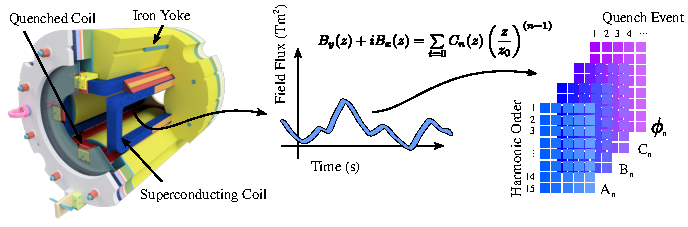
\includegraphics[width=\linewidth]{img/FieldProcedure.pdf}
	\caption{Sketch of the magnetic field measurements after a quench event for the quadrupole magnet and dataset obtained for each quench event measurement.}
	\label{fig:FieldMeasurement}
\end{figure}
We are interested in the resistive voltage buildup, that is why we use a voltage tap to split the
coil into two sub coils of the same size, the voltage of the coil can now be expressed as
\begin{equation}
	\label{eq:coil-voltage}
	\begin{aligned}
		 & \Delta V_T = \Delta V_1 + \Delta V_2 \enspace;       \\
		 & \text{where}                                         \\
		 & \Delta V_1 = \Delta V_{L1} + \Delta V_{R1} \enspace, \\
		 & \Delta V_2 = \Delta V_{L2} + \Delta V_{R2} \enspace.
	\end{aligned}
\end{equation}
The inductive voltage depends on the inductance $L$ (which is depends on the length, cross section
and number of turns of the equivalent solenoid) and the derivative of current intensity in time $I$,
which is negative because the current is lowered with time due to the requisite of having constant
total voltage~\footnote{
	During a quench we have a buildup of resistive voltage, which means that, since the voltage
	is kept constant by the power supply, the inductive decreases. The inductive voltage is
	computed as:
	\[\Delta V_L = L\dot{I} \enspace.\]
	Since the intensity of current decreases over time then the derivative $\frac{dI}{dt}$ must be negative.
}. In the ideal case we have that
\[\Delta V_{L1} + \Delta V_{R1} + \Delta V_{L2} + \Delta V_{R2} = - \Delta V_{L1} + \Delta V_{R1} -
	\Delta V_{L1} + \Delta V_{R2} = \Delta V_{R1} + \Delta V_{R2} \enspace.\]
This operation needs to be done for every pair of voltage taps in the magnet assmebly, leading to an
exponential complexity explosion. A more thorough analysis of the voltage measurement system can be
found in~\cite{mariotto2022-generic}.

In the original work, the condition of a superconducting coil was recognized based on the analysis of
the residual magnetic field. If the magnet was in working order, the residual magnetic field was
expected to be $\neq 0$. If one of the coils in the magnet assembly quenched, all the energy therein
contained would have been dumped on the resistance (due to the Quench Protection System activation),
therefore its residual magnetic field would be $\approx 0$. The asymmetrical behavior of the coils
changes the geometry of the residual magnetic field of the magnet at $0$ current, change that can be
detected using a quench antenna. Since the
quadrupoles, magnets MQSXF1 to MQSXF6, registered the majority of the quench events, due to their
high operating current, the original work focused on them and our work follows the same line. The
results of the test campaign were $279$ different measurements, only on quadrupoles, including those
identifying the magnet in good working condition, and quenches.

Harmonic decomposition of magnetic field, or multipolar expansion, is a classic technique used to
analyze magnetic field quality and is detailed in~\cite{ambrosio1996-mexpansion}. If we consider a
$2$D approximation of the magnet on the $X-Y$ plane, a point $z_0$ in the $X-Y$ plane and a current
$I$ flowing along the third axis $z$; the magnetic field $B(z_0)$ can be expressed as
\begin{equation}
	\label{eq:bz}
	|B(z_0)| = \frac{\mu_0I}{2\pi d} \enspace.
\end{equation}
Where $d$ is the distance between our point $z_0$ and the $z$ axis. The magnetic field can be
expressed as a complex number with the contribution along the $x$ axis and the contribution along
the $y$ axis
\begin{equation}
	\label{eq:bcomplex}
	\begin{aligned}
		 & B_z = 0 \enspace,         \\
		 & B  = B_x + iB_y \enspace.
	\end{aligned}
\end{equation}
Since we can express $z_0$ as a point in complex bidimensional space: $z_0 = x_0 + iy_0$, we can
rewrite~\ref{eq:bz} as the product of the modulus $|B(z_0)|$ and the versor normal to the segment $\overline{zz_0}$:
\begin{equation}
	\label{eq:bzcomplex}
	\begin{aligned}
		B & = B_x + iB_y                                              \\
		  & = \frac{mu_0I}{2\pi|z_0 - z|}\frac{i(z_0 - z)}{|z_0 - z|} \\
		  & = \frac{mu_0I}{2\pi}\frac{i}{z_0^* - z^*} \enspace.
	\end{aligned}
\end{equation}
Where $z^*$ and $z_0^*$ are, respectively, the conjugates of $z$ and $z_0$. Instead of using $B$ we
compute the its complex conjugate $B^*$
\begin{equation}
	\label{eq:bconj}
	\begin{aligned}
		 & B^* = B_x - iB_y = \frac{\mu_0I}{2\pi}\frac{i}{z - z_0} \enspace;           \\
		 & \text{since} \hspace{10pt} \left(\frac{i}{a + ib}\right)^* = \frac{i}{-(a +
			ib)^*} \enspace.
	\end{aligned}
\end{equation}
This because $B^*$ is an analytic function\footnote{
	An analytic function is a function that is locally given by a convergent power series. In
	general, a function is analytic if it respects the Cauchy Theorem which states the
	following: Let $D$ be a finite, simply connected domain and $C$ any closed, rectifiable curve contained in $D$. If the function $f(z)$ is differentiable in the domain $D$, then the integral of $f(z)$ along $C$ is equal to $0$. Which means that the function is analytic~\cite{evgrafov2019analytic}.
} which makes it more useful for two reasons:
\begin{itemize}
	\item we can expand it in power series, leading us to multipolar expansion (as we will see
	      in the following),
	\item for a given region, the maximum value of the modulus is on the boundary. This identifies the maximum field point within the magnet (even though $B^*$ is not analytic within the magnet we can use equivalent functions for it).
\end{itemize}
Since~(\ref{eq:bconj}) is analytic then we can do a power series expansion on $z$
\begin{equation}
	\label{eq:pexp}
	\frac{1}{z - z_0} = \frac{1}{z} \sum_{n = 1}^\infty \left(\frac{z_0}{z}\right)^n = \sum_{n =
		1}^\infty \frac{z_0^{n - 1}}{z^n} \enspace.
\end{equation}
We can rewrite~(\ref{eq:bconj}) for a uniformly distributed current density $J$ on an arbitrary
cross-section $\sigma$ as
\begin{equation}
	\label{eq:bconj-generic}
	B^* = i \frac{\mu_0J}{2\pi}\int_{\sigma}\frac{1}{z - z_0}da \enspace.
\end{equation}
If we apply the power-series expansion to the equation we just found:
\begin{equation}
	\label{eq:cn}
	\begin{aligned}
		 & B^*(z_0) = \sum_{n = 1}^\infty C_n z_0^{n - 1} \enspace,                        \\
		 & \text{with}\hspace{10pt}C_n = i \frac{\mu_0J}{2\pi}\int_{\sigma}\frac{1}{z^n}da
		\enspace .
	\end{aligned}
\end{equation}
The $C_n$ are non-normalized multipolar coefficients:
\begin{itemize}
	\item $C_1$ is the \emph{dipolar} field harmonic,
	\item $C_2$ is the \emph{quadrupolar} field harmonic,
	\item $C_3$ is the \emph{sextupolar} field harmonic;
\end{itemize}
and so on and so forth. The magnetic field can be described via an infinite amount of these
multipolar coefficients, any magnet aims at generating only one, but the resulting magnetic field is
never perfect. For instance: we would expect that a quadrupole only emits quadrupolar magnetic
field, but it introduces sextupolar, octupolar, \ldots disturbances.

Since the multipolar coefficient is a complex number it can be expressed as $C_n = A_n - iB_n$, the components
\begin{inparaenum}[(i)]
	\item $A_n$s generate the horizontal fields and are known as \emph{skew} components,
	\item $B_n$s generate the vertical fields and are called \emph{right} components.
\end{inparaenum}

Another formulation of field harmonics, which is still an analytic function, and is widely used, is
\begin{equation}
	\label{eq:ibz}
	iB^* = i (B_x - iB_y) = B_y - iB_x = i \left(\sum_{n = 1}^\infty{C_n z_0^{n - 1}}\right)
	\enspace.
\end{equation}
If we proceed to substitute the value for $C_n$ we identified above, we get the following
expression:
\begin{equation}
	\label{eq:fh}
	\begin{aligned}
		B_y - iB_x & = \sum_{n = 1}^\infty{(B_n + iA_n) z_0^{n - 1}} \\
		           & = B_0 \sum_{n = 1}^\infty({b_n + ia_n})
		\left(\frac{z_0}{R_{\text{ref}}}\right)^{n - 1} \enspace.
	\end{aligned}
\end{equation}
Where: $a_n$ and $b_n$ are the normalized multipoles, $B_0$ is the main \emph{right} multipolar
field (e.g., for a dipole $B_0 = b_1$, while for a quadrupole $B_0 = R_{\text{ref}}b_2$), and the $R_{\text{ref}}$ is the \emph{reference radius},
which renders the coefficients dimensionless and is usually taken as $2/3$ of the magnet aperture.

\medskip

During the test campaign, for each of the $279$ events, 60 samples of harmonic coefficients have
been measured and averaged to obtain a single set of $15$ different magnetic field harmonics
coefficients which contain all the information of the produced magnetic field quality (see
Fig.~\ref{fig:FieldMeasurement}). Recalling that these coefficients are expressed as complex
numbers, the information was organized in terms of the following four attributes, in which the suffix $n \in \{1, \dots,  15\}$ is related to a specific harmonic:
\begin{itemize}
	\item the skew component \an, of the $n^\text{th}$ field harmonic coefficient;
	\item the right component \bn, of the $n^\text{th}$ field harmonic coefficient;
	\item the absolute value \cnmod, of the $n^\text{th}$ field harmonic coefficient;
	\item the phase \phin, of the $n^\text{th}$ field harmonic coefficient.
\end{itemize}
Since the magnets in the original testing campaign were mounted skew; the $A_n$
feature was supposed to be highly informative since they are directly correlated with the rotational
position of the quenched coil in the magnet assembly. The modulus of~(\ref{eq:cn}) is
\begin{equation}
	\label{eq:cnmod}
	\begin{aligned}
		|C_n| & = \frac{\mu_0J}{2\pi} \sqrt{i \cdot i^*}\int_{\sigma}\frac{1}{|z^n|}da \\
		      & = \frac{\mu_0J}{2\pi} \int_{\sigma}\frac{1}{|z|^n}da \enspace.
	\end{aligned}
\end{equation}
If the coils are all positioned at the same distance from the origin and the only thing that
distinguishes them is the angular position, this information cannot be obtained starting from the
modulus of a complex number. For instance there is no way of distinguishing $i$ which corresponds to
$\pi / 2$ from $-i$, which corresponds to $3\pi / 3$.

Each measurement was coupled with a \emph{label} encoded as follows:
\begin{itemize}
	\item a simple binary flag for \qrp, where $1$ means that a quench has happened, while $0$ characterizes the normal working conditions of the superconductor;
	\item four binary flags for \qlp, each describing a  coil and stating whether or not a quench happened within it, using the same encoding as in previous point.
\end{itemize}
We remark here that the labels for \qrp\ were reasonably balanced: namely, the number of non-quench events was of $87$ while the number of quench events was of $192$; concerning \qlp, on the other hand, every coil has a different distribution: as detailed in Table~\ref{tab:balance}, the proportion of quench over non-quench events roughly ranges from $30\%$ to $50\%$. It is important to notice that the sum of all quench events for \qlp\ is not $192$, since one quench event for \qrp\ could have been caused by up to three different coils (e.g., coils 0, 1 and 3) quenching at the same time.

\begin{table}[h]
	\caption{Label distribution for the various coils in \qlp.}\label{tab:balance}

	\bigskip
	\setlength{\tabcolsep}{6pt}
	\centering
	\begin{tabular}{ccc}
		\toprule
		\textbf{Coil} & \textbf{Quench} & \textbf{Non-quench} \\
		\midrule
		0             & 68              & 211                 \\
		1             & 96              & 183                 \\
		2             & 79              & 200                 \\
		3             & 73              & 206                 \\
		\bottomrule
	\end{tabular}
\end{table}

In each of our experiments we did not use all attributes, in most cases the datasets aggregated the
best harmonics for a certain attribute (e.g., \an[2] and \an[12]). We will refer to these as sub-views of an attribute.

The objective of the thesis was to find machine learning models capable of recognizing:
\begin{enumerate}
	\item whether or not the magnet underwent a quench event during operation, which we will refer
	      to as Quench Recognition Problem (\qrp) from now on, and will be treated in \Cref{chp:qrp};
	\item which coil(s) transitioned, if the superconductor quenched; which we will refer to
	      as Quench Localization Problem (\qlp) from now on, and it will be treated in
	      \Cref{chp:qlp}.
\end{enumerate}
The models chosen to solve \qrp\ and \qlp\ had to be both reliable and highly explainable to favour
further study of quench phenomenon on High-Order corrector magnets.

\section{Model selection and model testing procedures}
Reproducibility is a key property of any experiment, to cover the basics, we set the seed for all
random number generators to the same value, and we used shared pipelines for all our experiments.

Sub-views are built using a common pipeline that generates three different datasets, serialized
for later reuse, an overview of the datasets is given here below.
\begin{itemize}
	\item The \emph{merged} dataset, \dm, which constructs a single table out of all the
	      measurements done on the attribute(s) for the different magnets. Before serialization, the
	      data is standardized.
	\item The \emph{blind-test} dataset, \db, contains a small part of the overall data available to us
	      ($29$ samples): these samples were kept locked until the experiments were considered
	      complete. Using the blind-test set we performed a final test on the best models to see
	      how well the performance generalized on unseen data.
	\item The \emph{reduced} dataset, \dr, contains the rest of the samples, $250$ in total,
	      and is the main set used to perform experiments.
\end{itemize}

Model selection and testing were carried out using Nested Cross Validation (\ncv). \ncv\ is suitable
for situations in which the data is not abundant~\cite{Larracy2021} due to its heavy reuse, enabling
model selection and testing; while also giving less biased performance estimates by averaging the
results on $k$ different folds. In the following section we will do a rapid ex-cursus on how the
cross-validation procedure works.

\subsubsection{Cross Validation}
\label{sec:cv}
In \Cref{chp:ml} we outlined the simple train-test splitting procedure, now we will introduce an
alternative technique that gives us a powerful tool to prevent overfitting and get less biased performance measures while also doing hyperparameter selection.

$k$-fold \cv~\cite{ZhouZhi-Hua2021ML} is a splitting technique that divides a dataset $D$ in $k$ different folds $\fold{i}, i \in \{1, \ldots, k\}$; the folds are non-overlapping and about the same size, therefore
\[\fold{i} \cap \fold{j} = \emptyset \hspace{5pt} \forall i, j \in \{1, \ldots, k\}, i \neq j \enspace,\]
and the union of all the folds is the original dataset
\[\bigcup_{i \in \{1, \ldots, k\}} \fold{i} = D \enspace.\]

In the framework of train-test splitting, if we used the procedure outlined in \Cref{sec:sml}, we
would:
\begin{inparaenum}[(i)]
	\item split the original dataset into the training set $T$ and the generalization set $G$,
	\item train a model $\model$ on $T$
	\item and then test the performance on $G$.
\end{inparaenum} While this is a perfectly acceptable procedure to gather performance metrics for a
model, it gives us reliable performance metrics only if the dataset is very large. The larger the
dataset $D$, the more samples can go in both $T$ and $G$; making sure that many different cases are
covered. If the dataset is small, like in our case, then it introduces a higher uncertainty on
performance metrics; meaning that it might be more likely that the generalization performance are
high due to a statistical anomaly.

By measuring performance on different folds (each one is a self-contained train-test procedure), we
get a more complete vision of the model performance: each sample in the dataset has been used
\emph{at least once} for training and \emph{one single time} for testing. The fold structure allows
us to recognize pathological situations, like cases in which the standard deviation of the fold
performance is very wide. To understand how the folds are constructed, let's consider an example in which $5$-fold \cv\ is computed on a dataset containing $250$ samples: $5$ different models are generated, each time trained on $200$ samples and then tested on the remaining $50$ samples (the testing fold changes with every iteration).

\smallskip

The number of folds to be used for \cv\ becomes a very important aspect of the problem, since it
depends on many factors like the amount of available data or the required reliability of performance
reads. A large value of $k$ will increase the number of folds the model is trained and tested on,
increasing the robustness of the performance estimation at the expense of computational complexity
(e.g., Leave One Out \cv\ is an example of such approaches, in~\cite{shao2016} a more efficient
approach to the technique is discussed); too small a value of $k$ makes the \cv\ less robust but more efficient (classic values of $k$ for most practical uses are $5, 10, 20$).

\smallskip

Let us now move to a more complicated environment in which we need, given a base model, to fine tune
it, train it and test it. We can na\"ively tripartition dataset $D$:
\begin{itemize}
	\item \emph{training set} $T$, which is the same set we defined in \Cref{sec:sml}, but is now
	      used to fine tune the hyperparameters of the model,
	\item \emph{validation set} $V$, this set will be used to test the performance of the model
	      found after hyperparameter selection,
	\item \emph{generalization set} $G$, after the model is retrained on $T \cup V$ the performance are
	      tested on $G$ to see if the model is capable of generalizing effectively.
\end{itemize}

Once again, we cannot guarantee that:
\begin{inparaenum}[(i)]
	\item the chosen model is the best one,
	\item the performance metrics obtained from the single generalization fold are actually reliable.
\end{inparaenum}
To address the issue we can substitute each procedure with $k$-fold \cv, one nested inside the other
one, the \emph{inner} is used to do model selection, the \emph{outer} is used to test performance
for the model just generated. To get a better understanding of the Nested cross-validation procedure
(\ncv) just introduced, let us consider a $5 \times 5$ \ncv\ procedure applied to a dataset of $250$
samples (an outline of the \ncv\ procedure is shown in \Cref{fig:nested-cv}).
\begin{enumerate}
	\item The data is first split into $5$ folds of $50$ samples. One fold of $50$ samples will
	      be kept on the side for the generalization test, the remaining $200$ samples will be
	      used to do both training and model selection. This is highlighted in
	      \Cref{fig:nested-cv} by the $5$ larger bars pointed by the arrows. The bright green
	      partitions are the ones used for training, while the red one is the one used for final
	      testing.
	\item For all possible combinations in the hyperparameter space~\footnote{
		      For all intents and pourposes we do not do a full exploration of the
		      hyperparameter space, because it's an infinite space. Therefore we do an
		      exploration of a user-defined hyperparameter grid (cfr. \Cref{tbl:params}).
		      Since we consider all the possibilities the computational complexity of such
		      exploration is exponential.\label{foot:hypr-grid}
	      } we repeat points 3 and 4.
	\item The training set is now split again in $5$ folds, $160$ samples will be used to do
	      model selection, $40$ samples will be used to validate the performance that has been
	      found. This is highlighted in \Cref{fig:nested-cv} by the $5$ smaller bars below each bar indicated in step 1.
	      The dark green partitions will be used to do training, while the bright green one
	      will be used to validate the performance metrics obtained.
	      In practice, as was anticipated in \Cref{sec:sml}, when we do model selection
	      (or hyperparameter fine-tuning) we explore only a very limited portion of the
	      hyperparameter space, and we select the combination that yields the best performance
	      during validation.
	\item Step 3 is repeated until all folds have been used for validation; in
	      \Cref{fig:nested-cv} we can see that each of the available partitions in the smaller
	      bars becomes bright green once before moving to the next iteration of the outer loop.
	      Since we use an hyperparameter grid (see footnote~\ref{foot:hypr-grid})\emph{De facto}, we used a hyperparameter grid (cfr. \Cref{tbl:params}), each combination yielded a different model that was later validated.
	\item The model found at the previous step is retrained on the whole $200$ training samples
	      (the green partitions in the larger bars in \Cref{fig:nested-cv}), and the
	      performance is tested on the fold that was kept aside in the first step (the red one
	      in \Cref{fig:nested-cv}).
	\item Steps 1, 2, 3, 4, 5 are repeated until every sample in the original dataset has been used
	      only one time for the final testing run. This is indicated in \Cref{fig:nested-cv}
	      by the fact that all the available partitions in the longer bars become red just
	      once.
\end{enumerate}
\begin{figure}[!t]
	\centering
	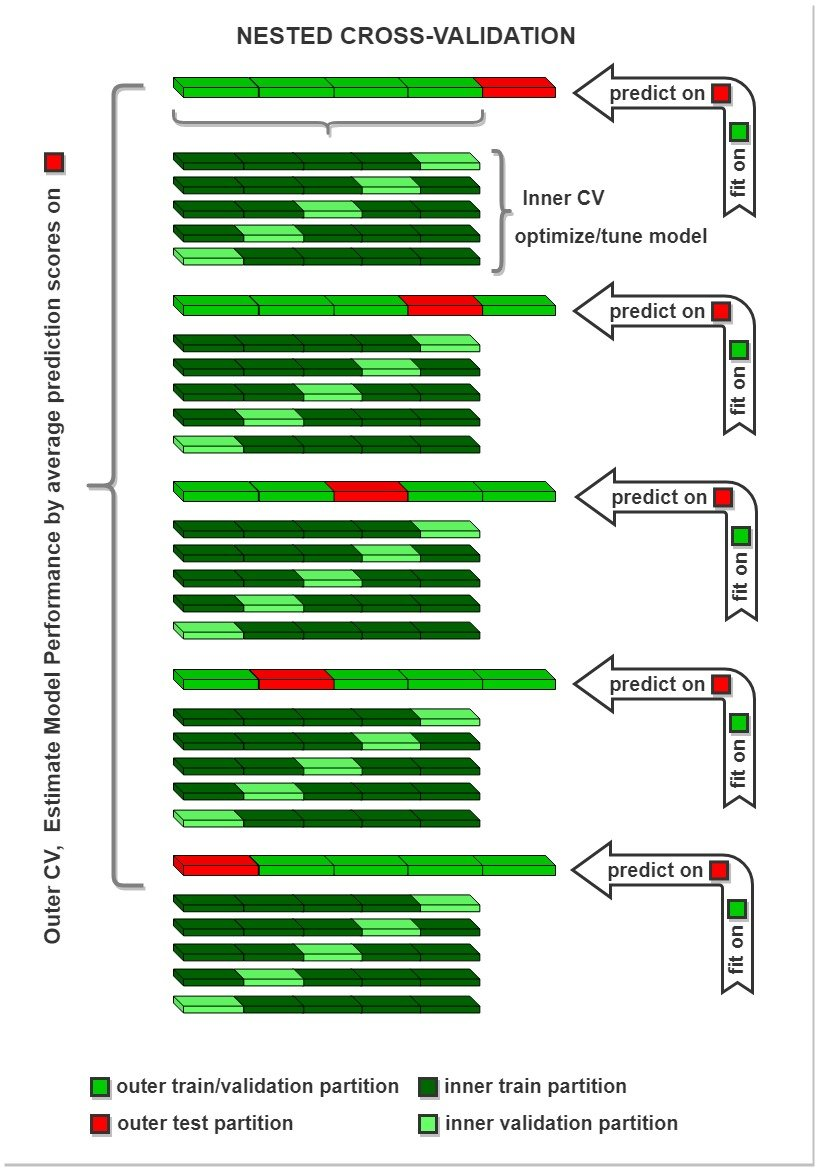
\includegraphics[scale=.3]{./img/nested-cv.png}
	\caption{Visualization of the nested cross validation procedure (taken
		from~\cite{lavasa2021}).}
	\label{fig:nested-cv}
\end{figure}

Once the \ncv\ procedure terminates we will get $k$ different models, since the fine-tuned models
are statistically equivalent, thus we can decide the one to keep based on the heuristic that fits our
objectives the best.

The closing section for this chapter will contain a summarization of the experimental setup.

\section{Experimental setup}
All experiments have been executed using Python 3.10.12 (the latest version at the time of writing), using the following libraries: scikit-learn (release 1.5.2) for data preprocessing and model training and evaluation, numpy (release 2.2.3) for efficient data storage, and Pandas (release 2.2.3) for data management. These libraries have been handled through the pip package manager (release 25.0.1) and used within a virtual environment.

The seeds from the various random number generators have been set to the common value of
\href{https://www.google.com/search?q=the+answer+to+life+the+universe+and+everything&num=10&client=firefox-b-d&sca_esv=a81abf9bb67ffd9b&sxsrf=AHTn8zo6RKep_zuEvIhJb5nuAGh5xAERLg\%3A1739739141586&ei=BVCyZ_C9I9mLi-gP7e-B8Ac&oq=the+answer+to+&gs_lp=Egxnd3Mtd2l6LXNlcnAiDnRoZSBhbnN3ZXIgdG8gKgIIADIIEAAYgAQYywEyCBAAGIAEGMsBMgUQABiABDIIEAAYgAQYywEyCBAAGIAEGMsBMggQABiABBjLATIIEAAYgAQYywEyCBAAGIAEGMsBMggQABiABBjLATIIEAAYgAQYywFIjCJQqQlYiRlwA3gBkAEAmAFuoAHICaoBBDExLjO4AQPIAQD4AQGYAhGgAv0JwgIKEAAYsAMY1gQYR8ICChAjGIAEGCcYigXCAgsQABiABBixAxiDAcICCxAuGIAEGLEDGIMBwgIOEC4YgAQYsQMY0QMYxwHCAg4QLhiABBixAxiDARiKBcICERAuGIAEGLEDGNEDGIMBGMcBwgIMECMYgAQYExgnGIoFwgIEECMYJ8ICDRAuGIAEGEMY1AIYigXCAgoQABiABBhDGIoFwgIOEC4YgAQYxwEYjgUYrwHCAgoQLhiABBhDGIoFwgIIEC4YgAQYsQPCAggQABiABBixA8ICCxAuGIAEGLEDGNQCwgIFEC4YgATCAggQLhiABBjLAcICCxAuGIAEGNEDGMcBmAMAiAYBkAYIkgcEMTIuNaAHrboC&sclient=gws-wiz-serp}{42}
ensure replicability of the experiments.

The original dataset contained $279$ samples: for \qrp, each sample consisted of $15$ harmonics and
a label, stating whether the sample represents a quench event ($1$) or not ($0$); while for \qlp each sample had $4$ different
labels associated to it representing whether each one of the coils ($0$ for East, then: North, West and
South) quenched ($1$) or not ($0$).

Every splitting operation was performed by stratifying on the labels, in the case of \qlp, if the
labels were more than one, we used a multi-class stratification technique, detailed in~\cite{skmlearn}.

Experiments were conducted on three different computers running different architectures and
different operating systems, but the results did not change due to the standard-oriented approach.
See \Cref{tbl:computers} for a summary of the computers we used.
\begin{table}[!ht]
	\caption{System configuration used for our experiments. Core count values are detailed as number
		of CPU cores and threads, while frequency is expressed in the base and boost specifications.
		Finally, the CPU cache size is shown for the L1, L2 and L3 levels, where
		available.}\label{tbl:computers}

	\bigskip

	\centering
	\setlength{\tabcolsep}{4pt}
	\begin{tabular}{lccc}
		\toprule
		                     & \textbf{Pigna}        & \textbf{Mattone}         & \textbf{Topone}    \\
		\midrule
		\textbf{Model}       & Macbook Pro           & Custom build             & Dell XPS 8700      \\
		\textbf{CPU}         & i$5$ $5287\textsc{u}$ & Ryzen 7 $3700\textsc{x}$ & i$7$ $4770$        \\
		\textbf{Core count}  & $2\cc / 2\tds$        & $8\cc / 16\tds$          & $4\cc /
		8\tds$                                                                                       \\
		\textbf{Launch Date} & Q$1$ 2015             & Q$2$ 2019                & Q$2$ 2013          \\
		\textbf{Frequency}   & $2.90 / 3.30$ \ghz    & $4.125 / 4.40$ \ghz      & $3.40 / 3.90$ \ghz \\
		\textbf{Cache}       & $3$ \mb               & $0.512 / 4 / 32$ \mb     & $8$ \mb            \\
		\textbf{TDP}         & $28$ \w               & $84$ \w                  & $65$ \w            \\
		\textbf{RAM}         & $8$ \gb               & $16$ \gb                 & $16$ \gb           \\
		\textbf{OS}          & Pop!\_OS $22.04$ LTS  & Pop!\_OS $22.04$ LTS     & Fedora $39$        \\
		\bottomrule
	\end{tabular}
\end{table}
Experiments were dispatched on different systems based on the expected computational load.

Model selection was handled by doing a partial exploration of the parameter space (as mentioned in
\Cref{sec:cv}) via a grid search algorithm (GridSearchCV in scikit-learn), in which each model we defined a custom parameter grid (shown in \Cref{tbl:params}).

\begin{table}[!ht]
	\caption{Hyperparameters which we have tuned during the model training phase.} \label{tbl:params}

	\bigskip

	\centering
	\setlength{\tabcolsep}{6pt}
	\begin{tabular}{llc}
		\toprule
		\textbf{Model}       & \textbf{Hyperparameter}                                           & \textbf{Values}                        \\
		\midrule
		\multirow{5}{*}{DT}  & impurity criterion                                                & gini, entropy, log loss                \\
		                     & max depth                                                         & $2, 3, 4, 5$                           \\
		                     & min impurity decrease                                             & $0.001, 0.01, 0.05$                    \\
		                     & max features                                                      & None, $0.5, 0.75$                      \\
		                     & min samples leaf                                                  & $5, 10, 20$                            \\
		\midrule
		\multirow{2}{*}{RF}  & n. of trees                                                       & $2, 3, 5, 10$                          \\
		                     & \multicolumn{2}{l}{$+$ the same hyperparameters and values of DT}                                          \\
		\midrule
		\multirow{5}{*}{SVC} & $C$                                                               & $0.1, 1, 10, 100, 1000$                \\
		                     & $\gamma$                                                          & scale, auto, $0.001, 0.01, 0.1, 1, 10$ \\
		                     & degree                                                            & $2, 3, 4, 5$                           \\
		                     & $c_0$                                                             & $0, 0.1, 0.5, 1$                       \\
		                     & kernel                                                            & linear, poly sigmoid, rbf              \\
		\bottomrule
	\end{tabular}
\end{table}

All models have been tested on a suite of scorers meant to give us a more complete
understanding of how well the model is performing. The metrics are explained here below and, as
usual, by positive (negative) sample we mean a sample having label $1$ ($0$), and by true (false)
positive we mean a correctly classified positive (negative) sample:
\begin{itemize}
	\item \emph{Accuracy} (Acc): fraction of correct predictions,
	\item \emph{Precision} (Prc): number of true positives over number of positive predictions,
	\item \emph{Recall} (Rec): number of true positives over number of positive items,
	\item \emph{F1 score} (F1): harmonic mean between Precision and Recall,
	\item \emph{Inverse recall} (Irec): number of true negatives over number of negative items,
	\item \emph{ROC AUC} (RAUC): area under the ROC curve, the higher the value the further the
	      model is from being a random classifier.
\end{itemize}
Among all metrics we chose accuracy as the one leading model selection and main scorer since it
gives us a rough idea of the model performance: a high accuracy means that the model is
capable of recognizing well both positives and negatives. While this metric alone cannot tell us the
whole story (for instance, with a very high accuracy that is only sending $1$ as output), is a very
good large-grain metric. Any finer analysis can be done using the other metrics just described.
Furthermore the dataset (as we saw earlier in this chapter) is essentially balanced, therefore we didn't
have any particular necessities to cover.






\chapter{Quench Recognition Problem (QRP)}
\label{chp:qrp}
This chapter is dedicated to the solution of \qrp, which we introduced in \Cref{chp:problem}, in this chapter we will:
\begin{itemize}
	\item Give a rapid overview of the problem, analyzing the results obtained from
	      preprocessing.
	\item Talk about the models used, and the results obtained for each model.
	\item Select the 'best' possible model.
\end{itemize}

\section{Data preprocessing}
\label{sec:qrp-preprocessing}
Before working on the actual models we analyzed:
\begin{itemize}
	\item The cross-correlation among harmonics of a specific attribute, which aims to identify repeated
	      information within it.
	\item The cross-correlation between the harmonics and the labels, which indicates how
	      well harmonics for a certain attribute are capable of explaining the expected results.
	\item The box-plot of the attributes, which visualizes the variability of the harmonics,
	      giving us a powerful tool to understand which ones are more relevant to the
	      computation.
	\item Visualization of the data after a run of dimensionality reduction via principal component
	      analysis (\pca), which could give us an idea of which are the better attributes to solve the problem.
\end{itemize}
In the following, the vector containing the information about the correlation with the labels has
been plotted after a normalization step (see \Cref{eq:normalization}~\cite{Nishok2024}). While this
procedure doesn't change the intensity of the correlation between harmonics and labels, it
makes the plots more readable and easier to interpret.
\begin{equation}
	\label{eq:normalization}
	X_\text{scaled} = \frac{X - X_\text{min}}{X_\text{max} - X_\text{min}}
\end{equation}
Where $X$ is a sample in the vector that is being scaled.

We will be covering the results of preprocessing in four different sections, each dedicated to a
specific attribute.

\subsubsection{\an}
\Cref{fig:an-corr} highlights the correlation among the harmonics of attribute \an. Independently of
the sign, the matrix evidently contains a pattern, hinting to the fact that many harmonics contain
repeated information, (e.g., \an[1] provides the same information as \an[3], \an[5], \an[7]), \ldots
By analyzing the figure we can reach the following conclusions:
\begin{itemize}
	\item Its strong geometry implies that doing feature extraction is going to be complex (as
	      we will see in the following sections it's basically a shared characteristic for
	      almost all the attributes) due to the necessity of finding a mix of harmonics that
	      has a high correlation with the label, while having a low correlation among
	      themselves.o
	\item All the odd harmonics are strongly correlated with each other (with the sole exception
	      of \an[15]),
	\item \an[2] is strongly correlated with its odd multiples (i.e., \an[6], \an[10], \an[14]),
	\item \an[4] is strongly correlated with all its multiples (i.e., \an[8], \an[12]),
	\item \an[15] is the only one not correlated to any of the other harmonics.
\end{itemize}
\begin{figure}[!ht]
	\centering
	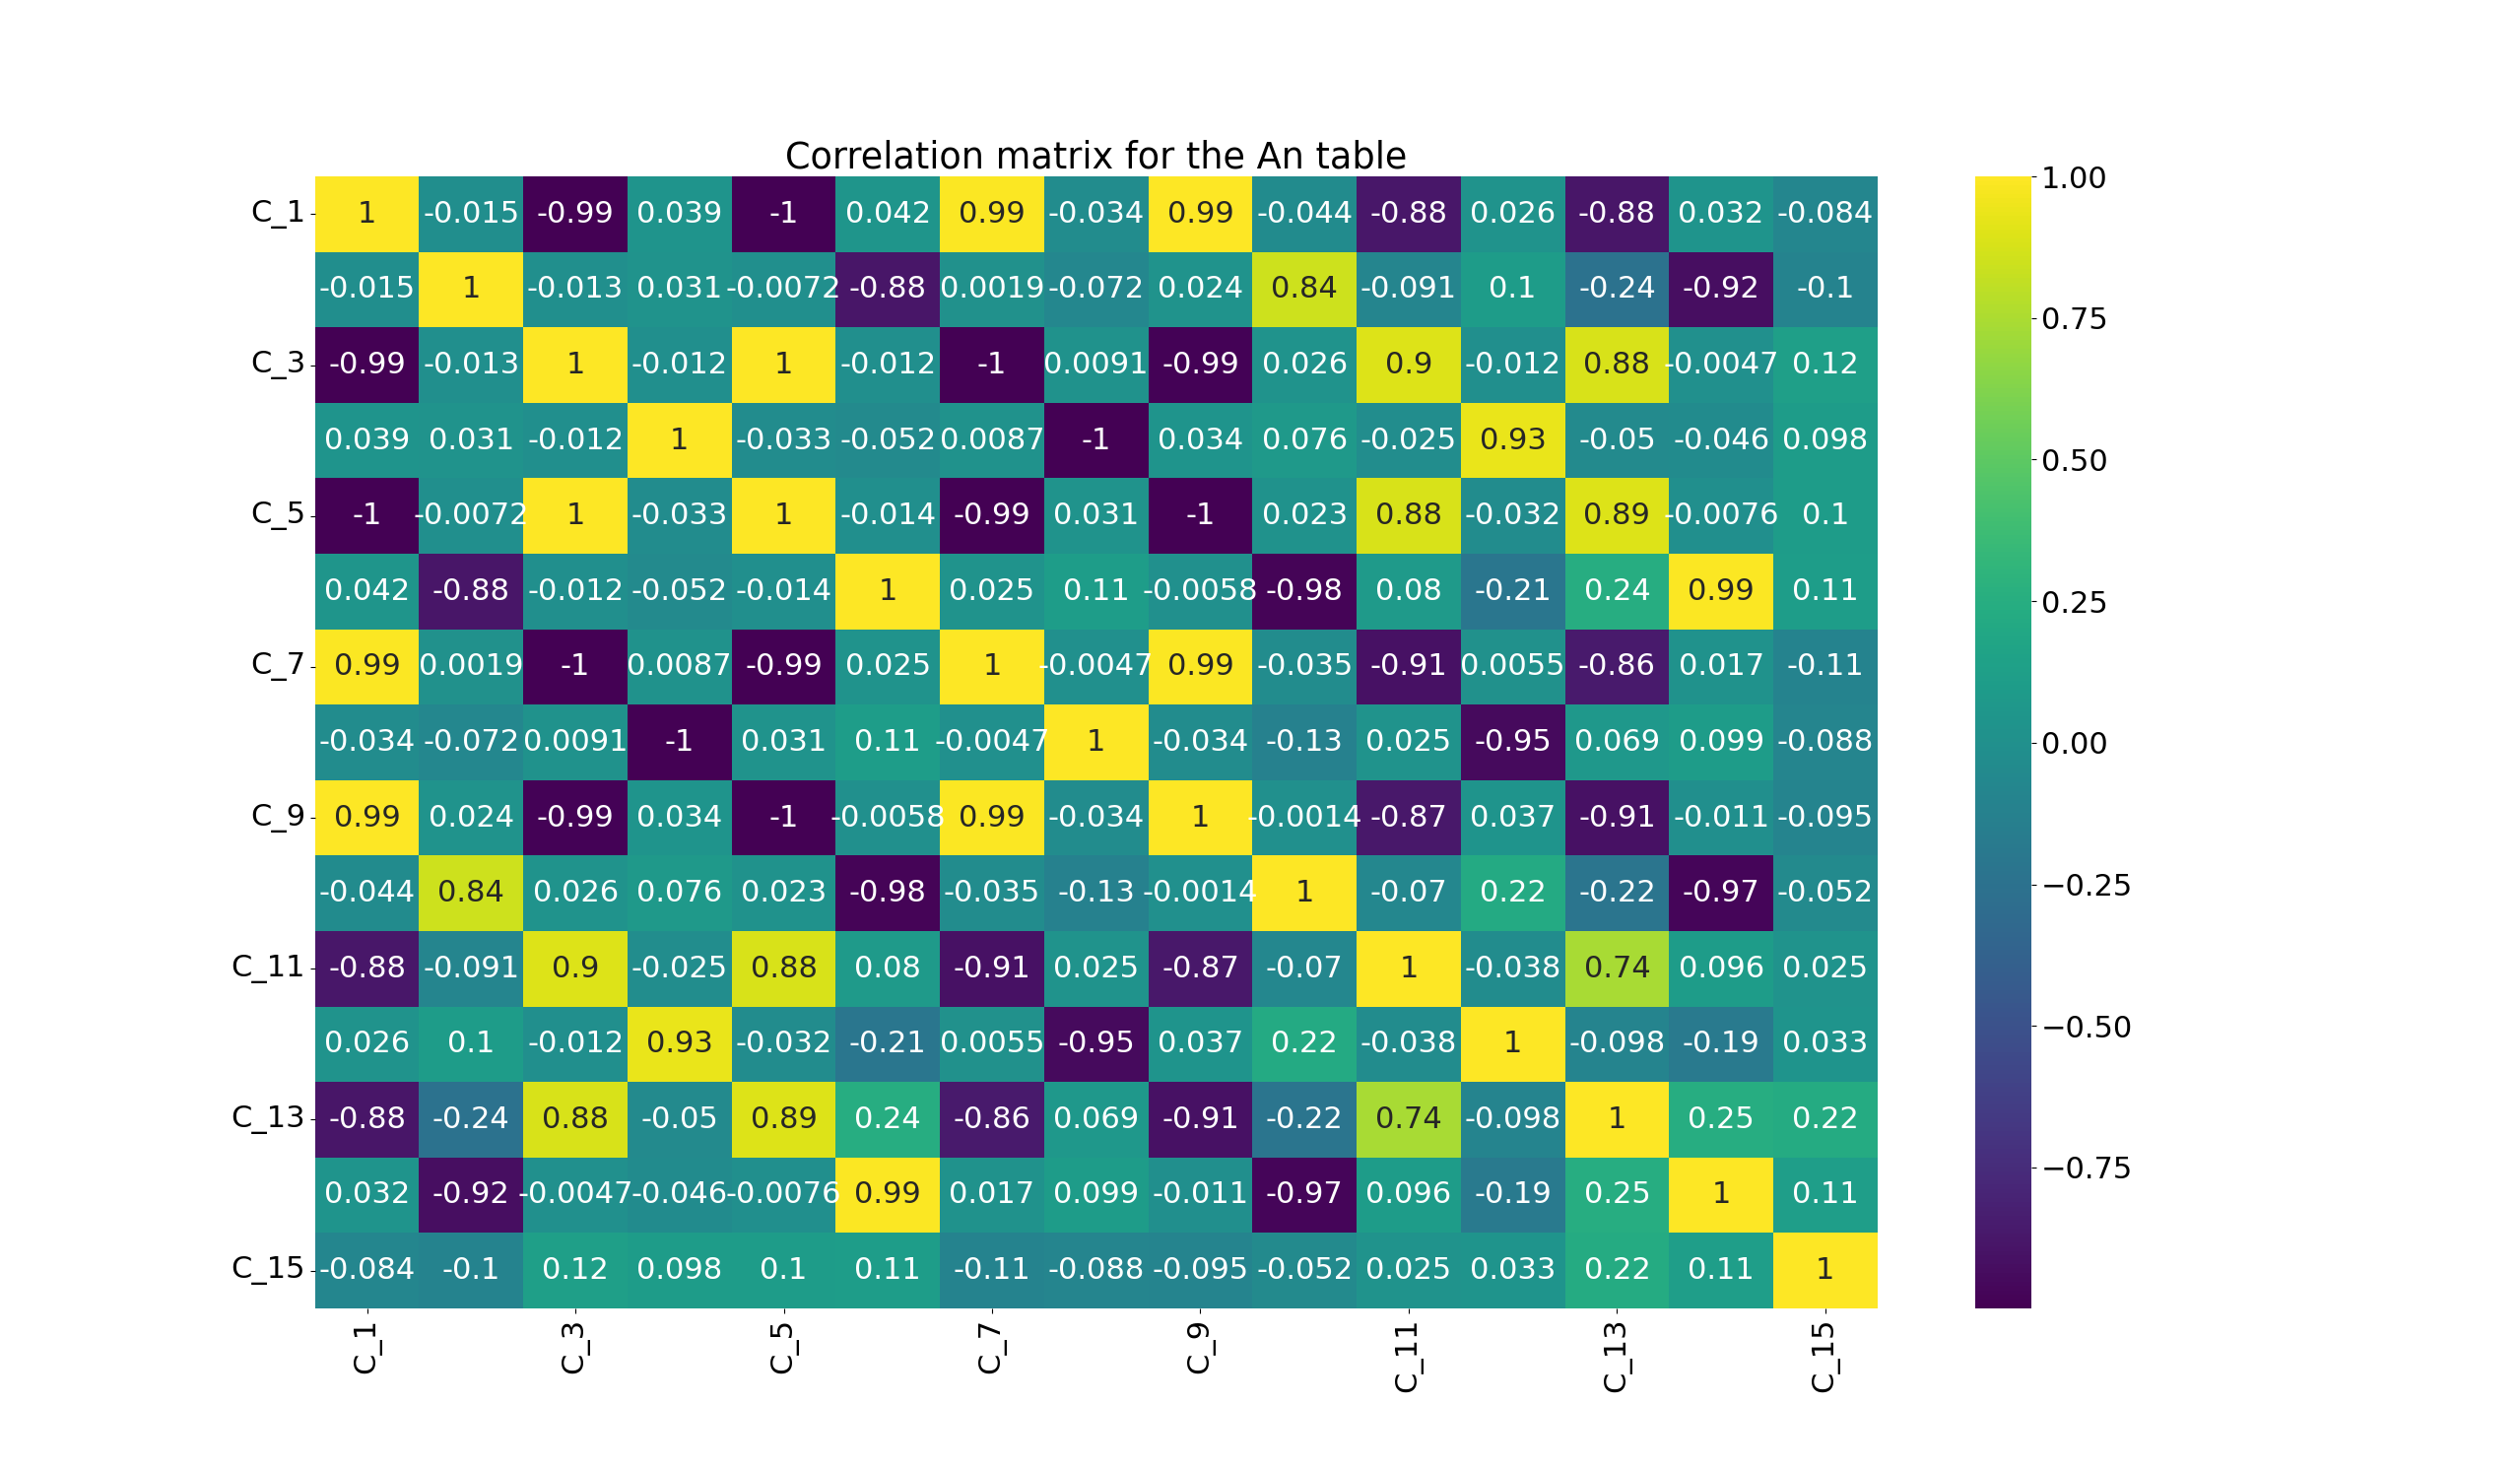
\includegraphics[width=\linewidth]{img/An_corr_matrix.png}
	\caption{The cross-correlation among the \an\ harmonics. The higher the color intensity
		(close to yellow or purple) the higher the correlation among the different harmonics.} \label{fig:an-corr}
\end{figure}

In \Cref{fig:an-lcorr} we plotted the correlation between the harmonics and the labels. If we pick
the harmonics with the highest label correlation, identified by a higher color intensity, we end up
with the following features, in order: \{\an[2], \an[6], \an[10], \an[11], \an[12], \an[13], \an[14],
\an[15]\}. This is interesting because:
\begin{enumerate}
	\item \an[2], as well as its odd multiples, can explain the results well, which is what we
	      expect from the theory (since the second harmonic is fundamental for the quadrupole).
	\item High order harmonics are able to explain the results better than other harmonics,
	      which is not what we would have expected, since in the original analysis the value for the
	      labels was computed using primarily low-order harmonics\footnote{
		      By low order harmonics we intend the harmonics going from $1$ to $6$ circa
	      }.
\end{enumerate}

\begin{figure}[!ht]
	\centering
	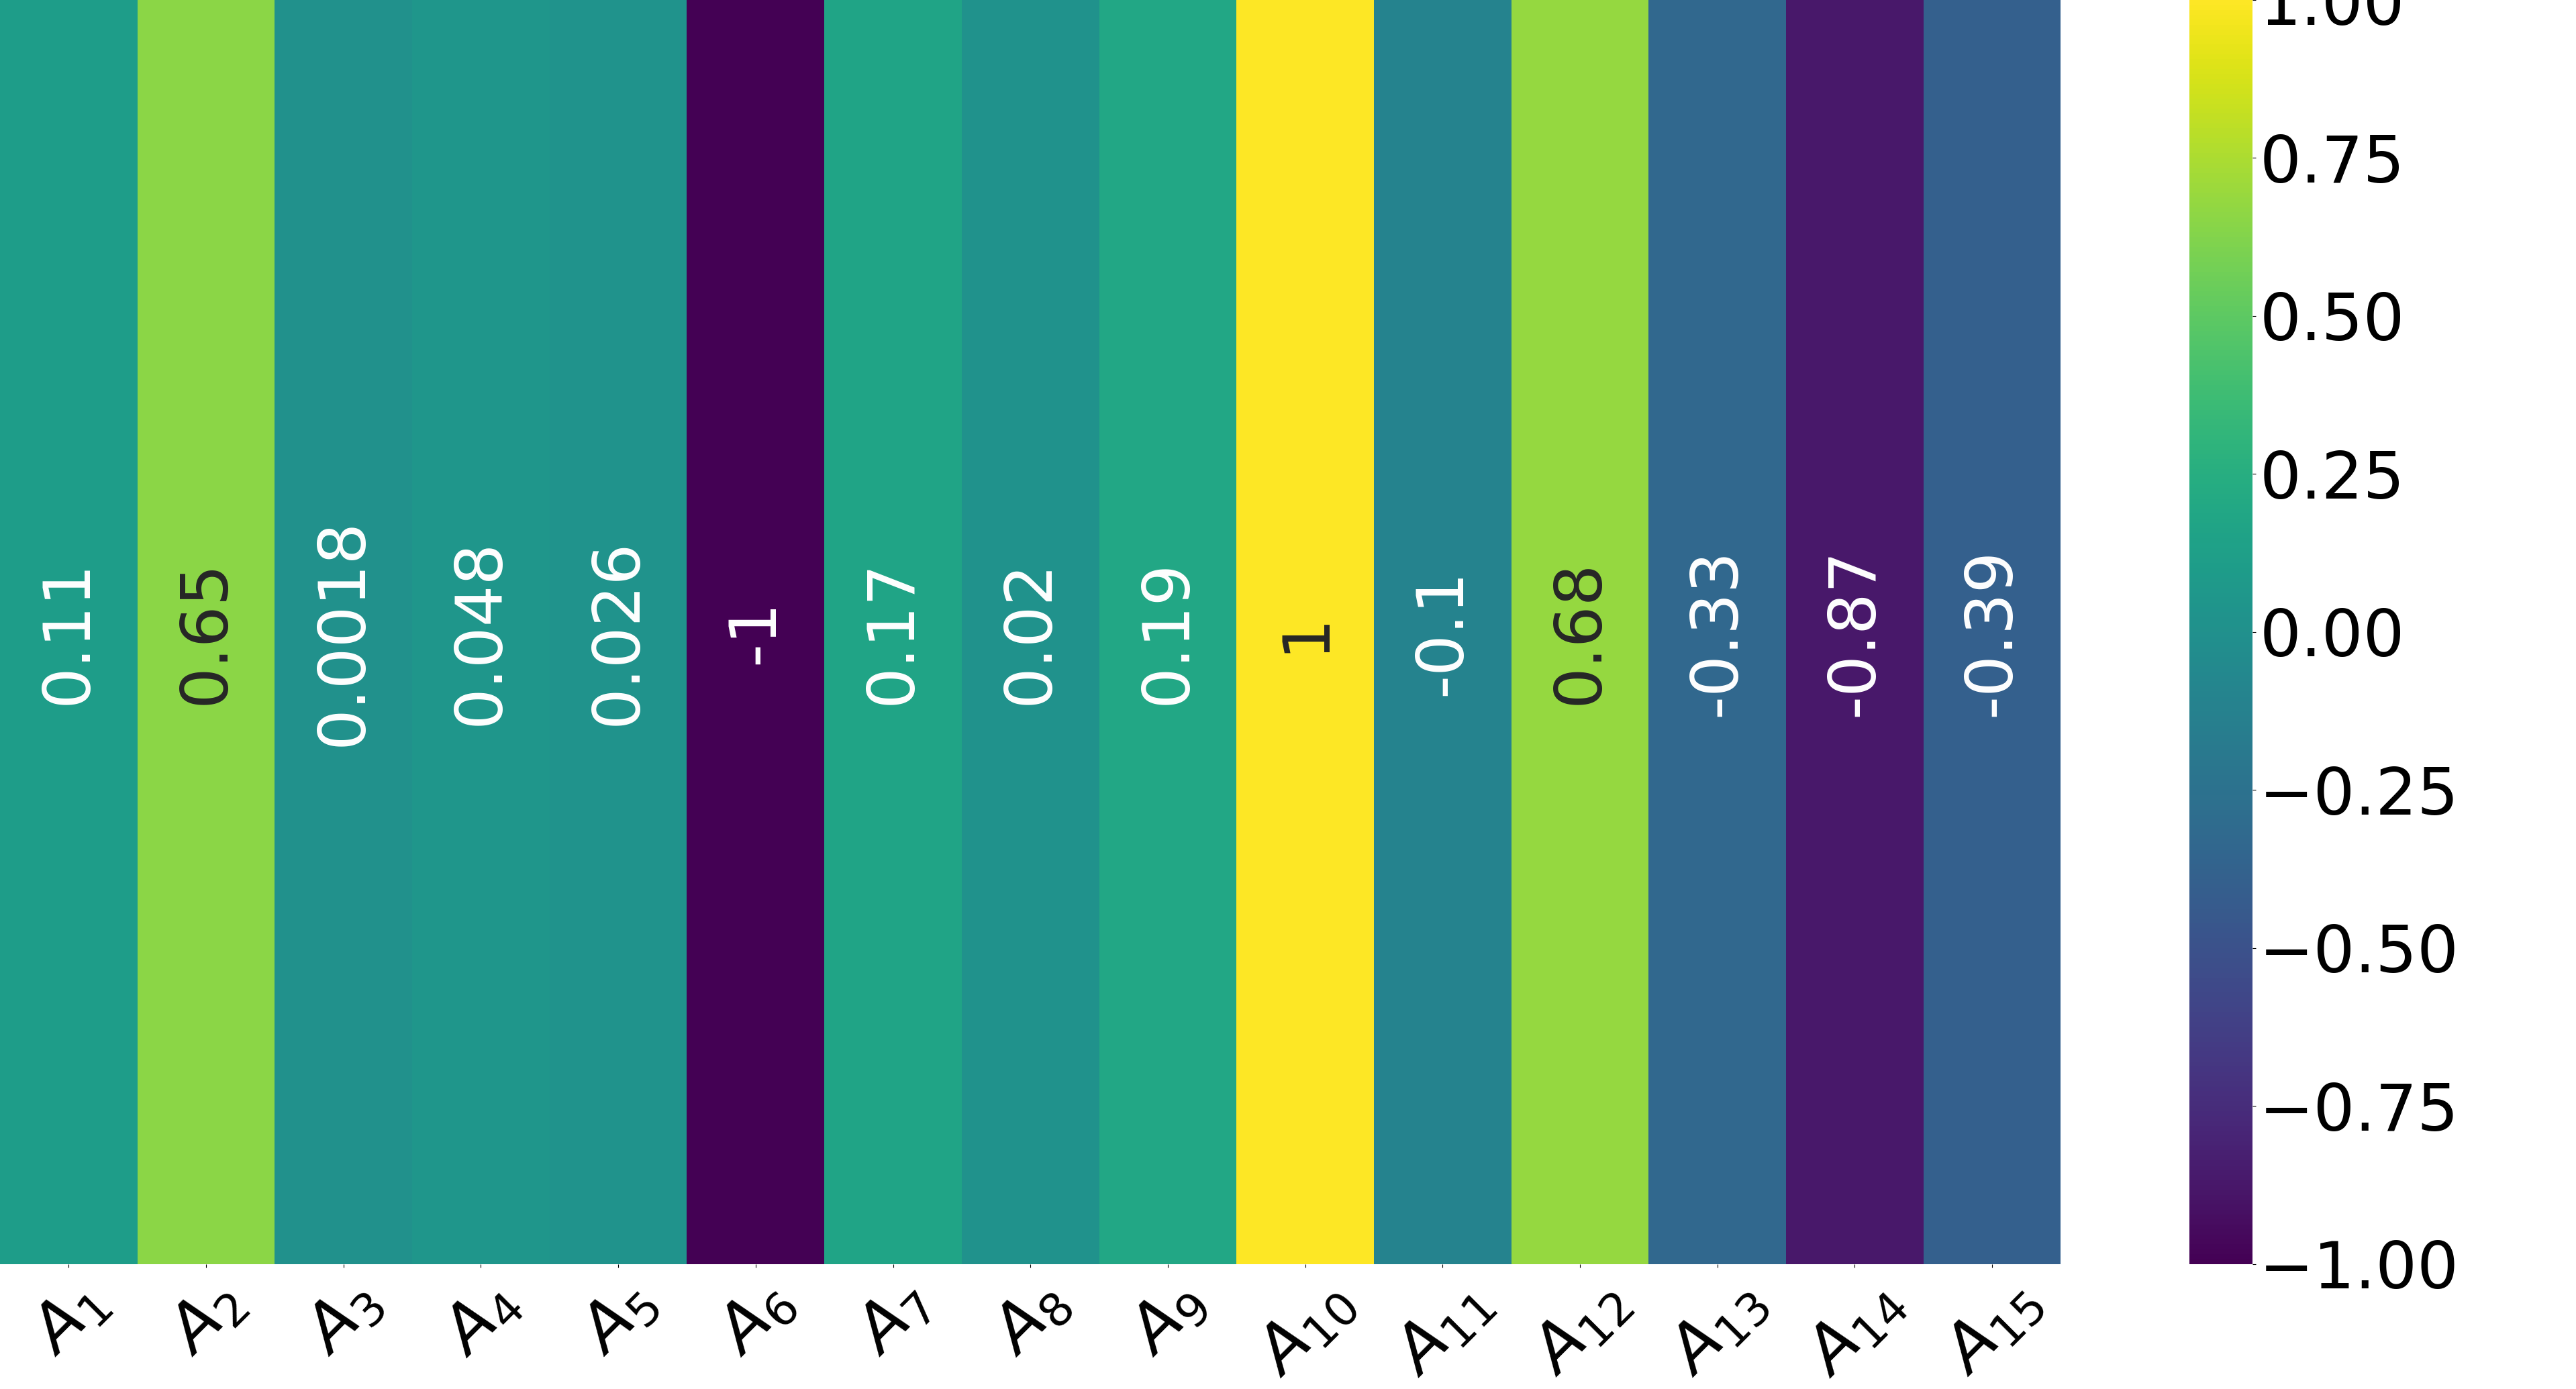
\includegraphics[width=0.7\linewidth]{img/An_label_corr.png}
	\caption{Correlation between the harmonics and the labels for \an.} \label{fig:an-lcorr}
\end{figure}

The structure of the correlation matrix and the correlation between labels and harmonics leads us to
believe that a good-performing sub-view for \an\ should contain \an[2], or one of its high-order
odd multiples, as well as \an[15]\ and some other high-order harmonics like \an[11]\ or \an[13].

Lastly, we can visualize the distribution of samples in bidimensional space, achieved by using \pca\
dimensionality reduction.
\begin{figure}[!ht]
	\centering
	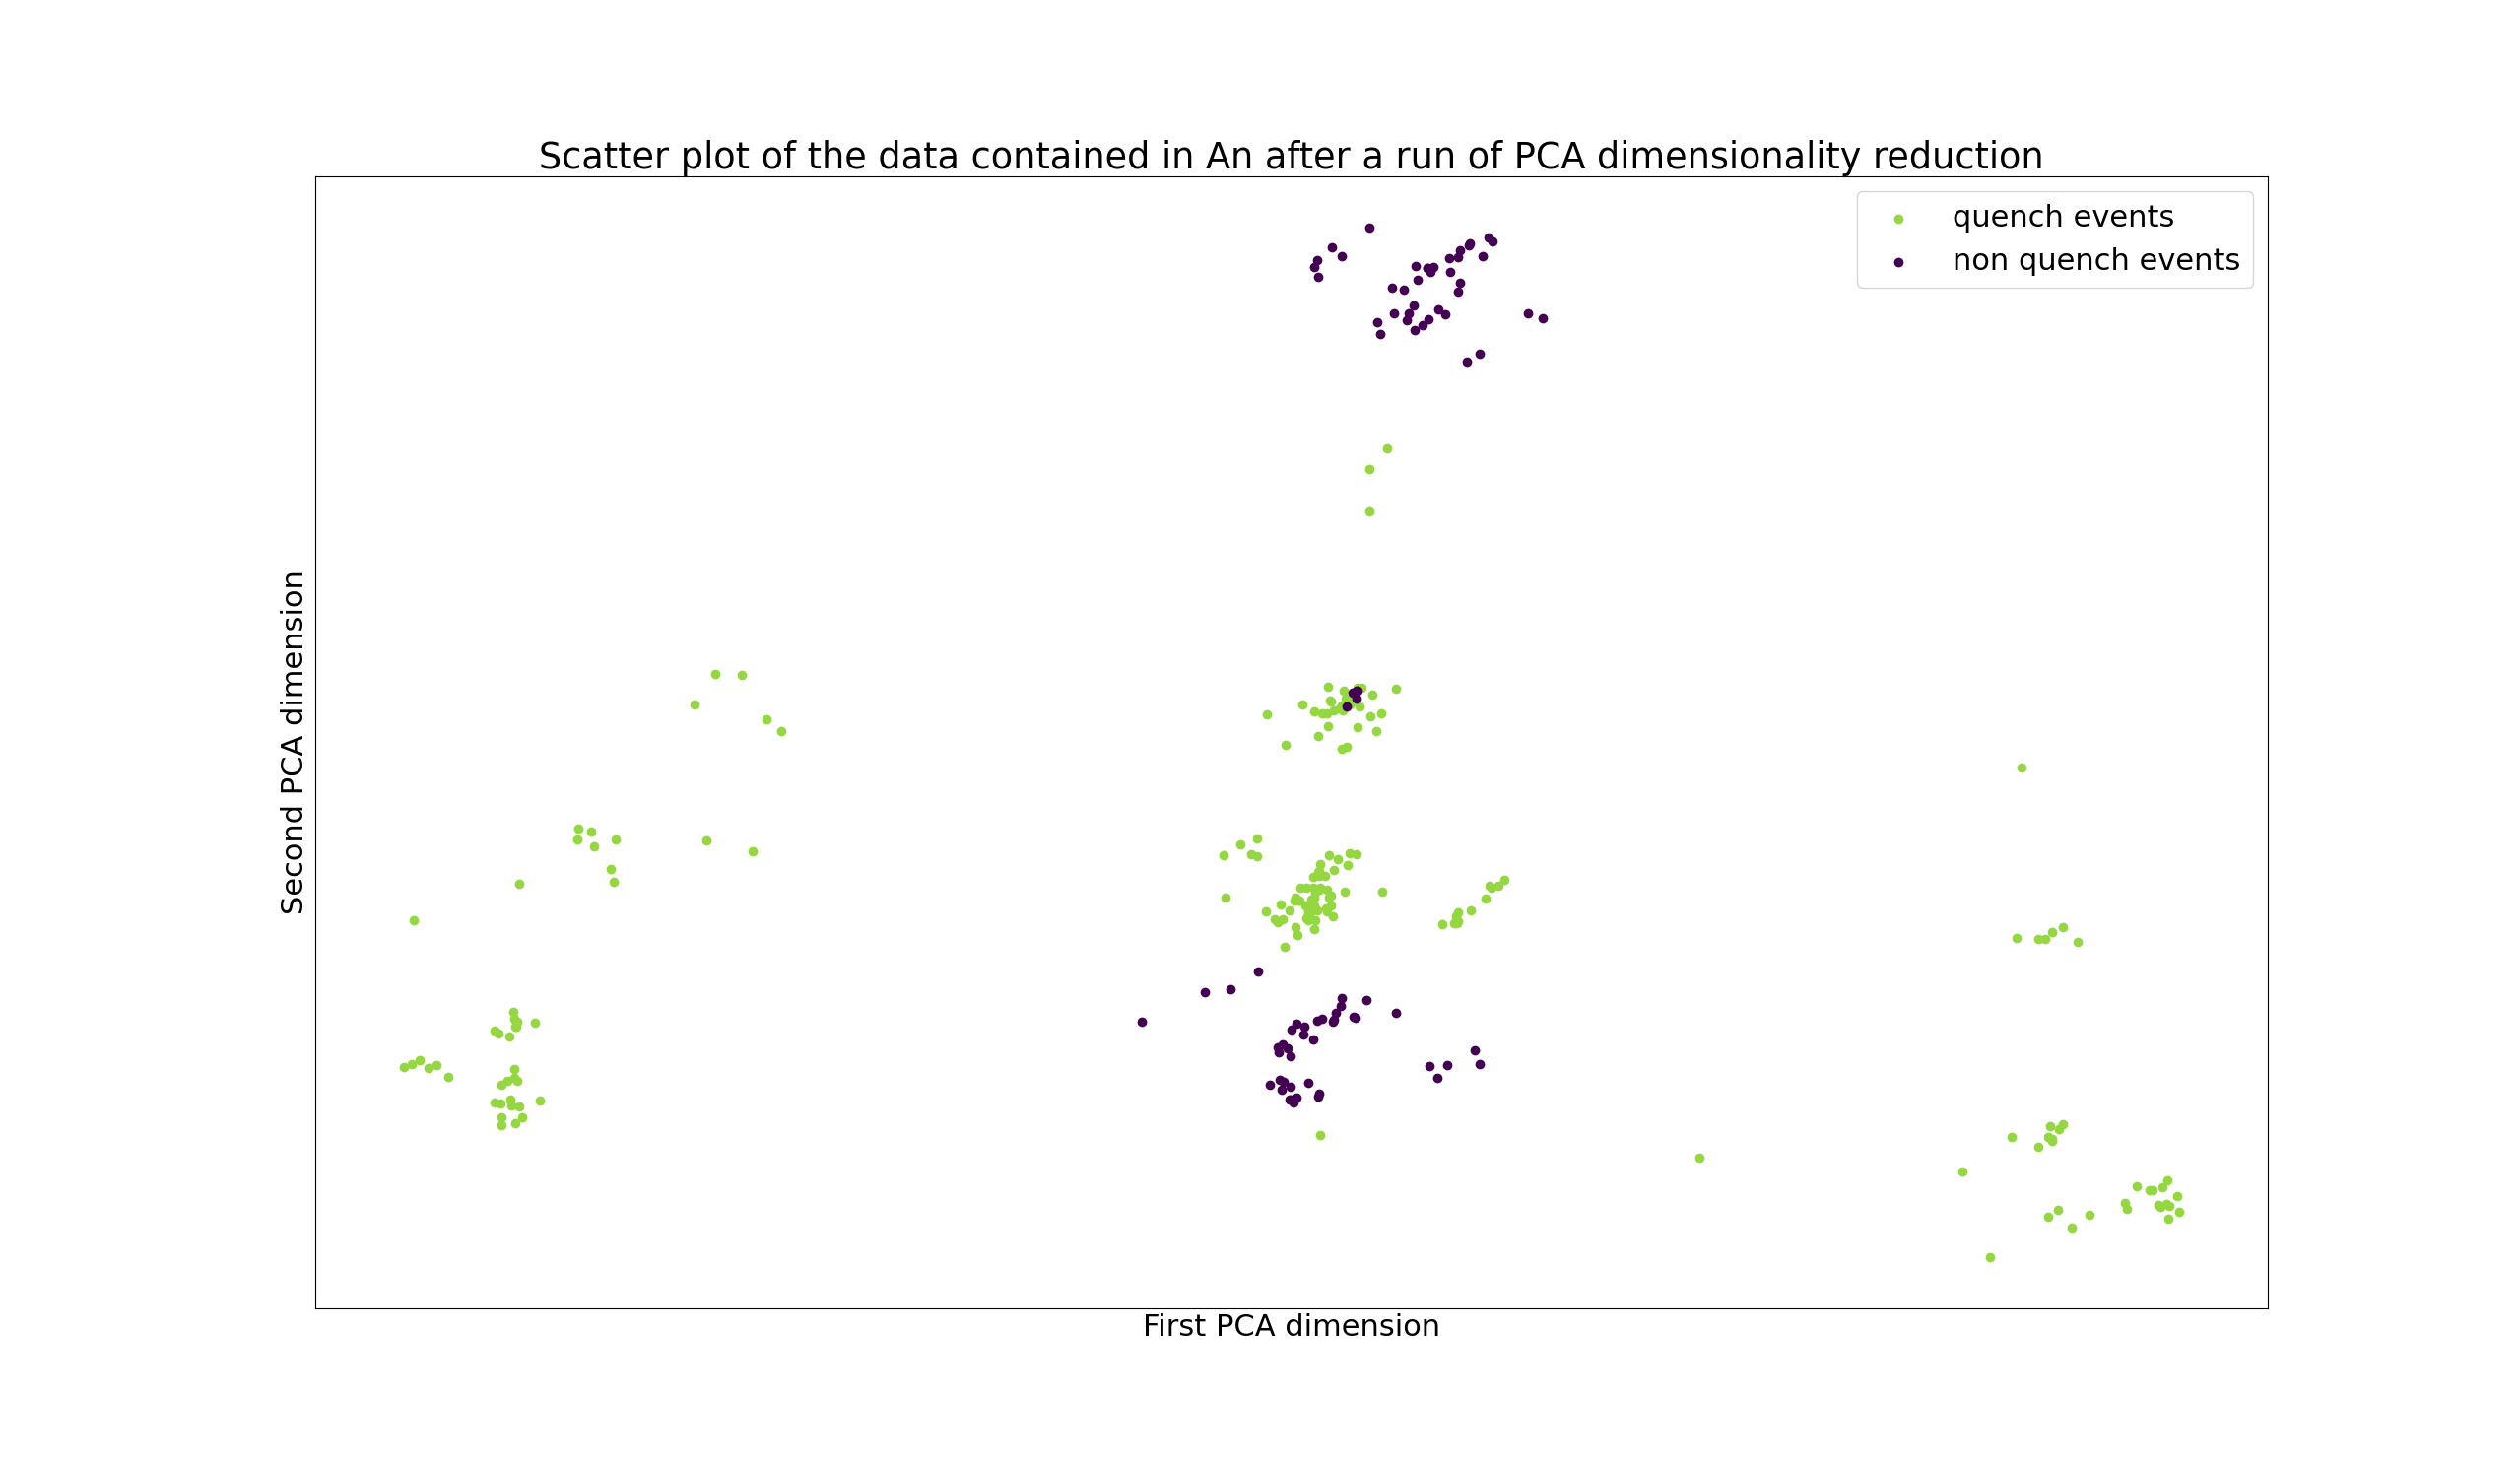
\includegraphics[width=0.7\linewidth]{img/An_distribution.png}
	\caption{Data distribution for the \an\ table after applying \pca\ dimensionality reduction,
		moving from $15$-dimensional space to $2$-dimensional space. In the plot we highlight quench
		and non-quench events.} \label{fig:an-dist}
\end{figure}

As we will see in \Cref{sec:qlp-cluster}, the visualization just shown is the best available (apart
from the one for \cnmod). Having such a good distribution lead us to think that it might be the reason why
models built on \an\ and \cnmod\ (at least for \qrp) perform better than the ones built on \bn\ and
\phin.

\subsubsection{\bn}
We can use a similar procedure on the \bn\ attribute, which in most tests proved to be the
least-performing attribute. This is probably due to the very poor distribution of the data, as we can see in
\Cref{fig:bn-dist}, the central cluster has a very high level of homogeneity.
\begin{figure}[!ht]
	\centering
	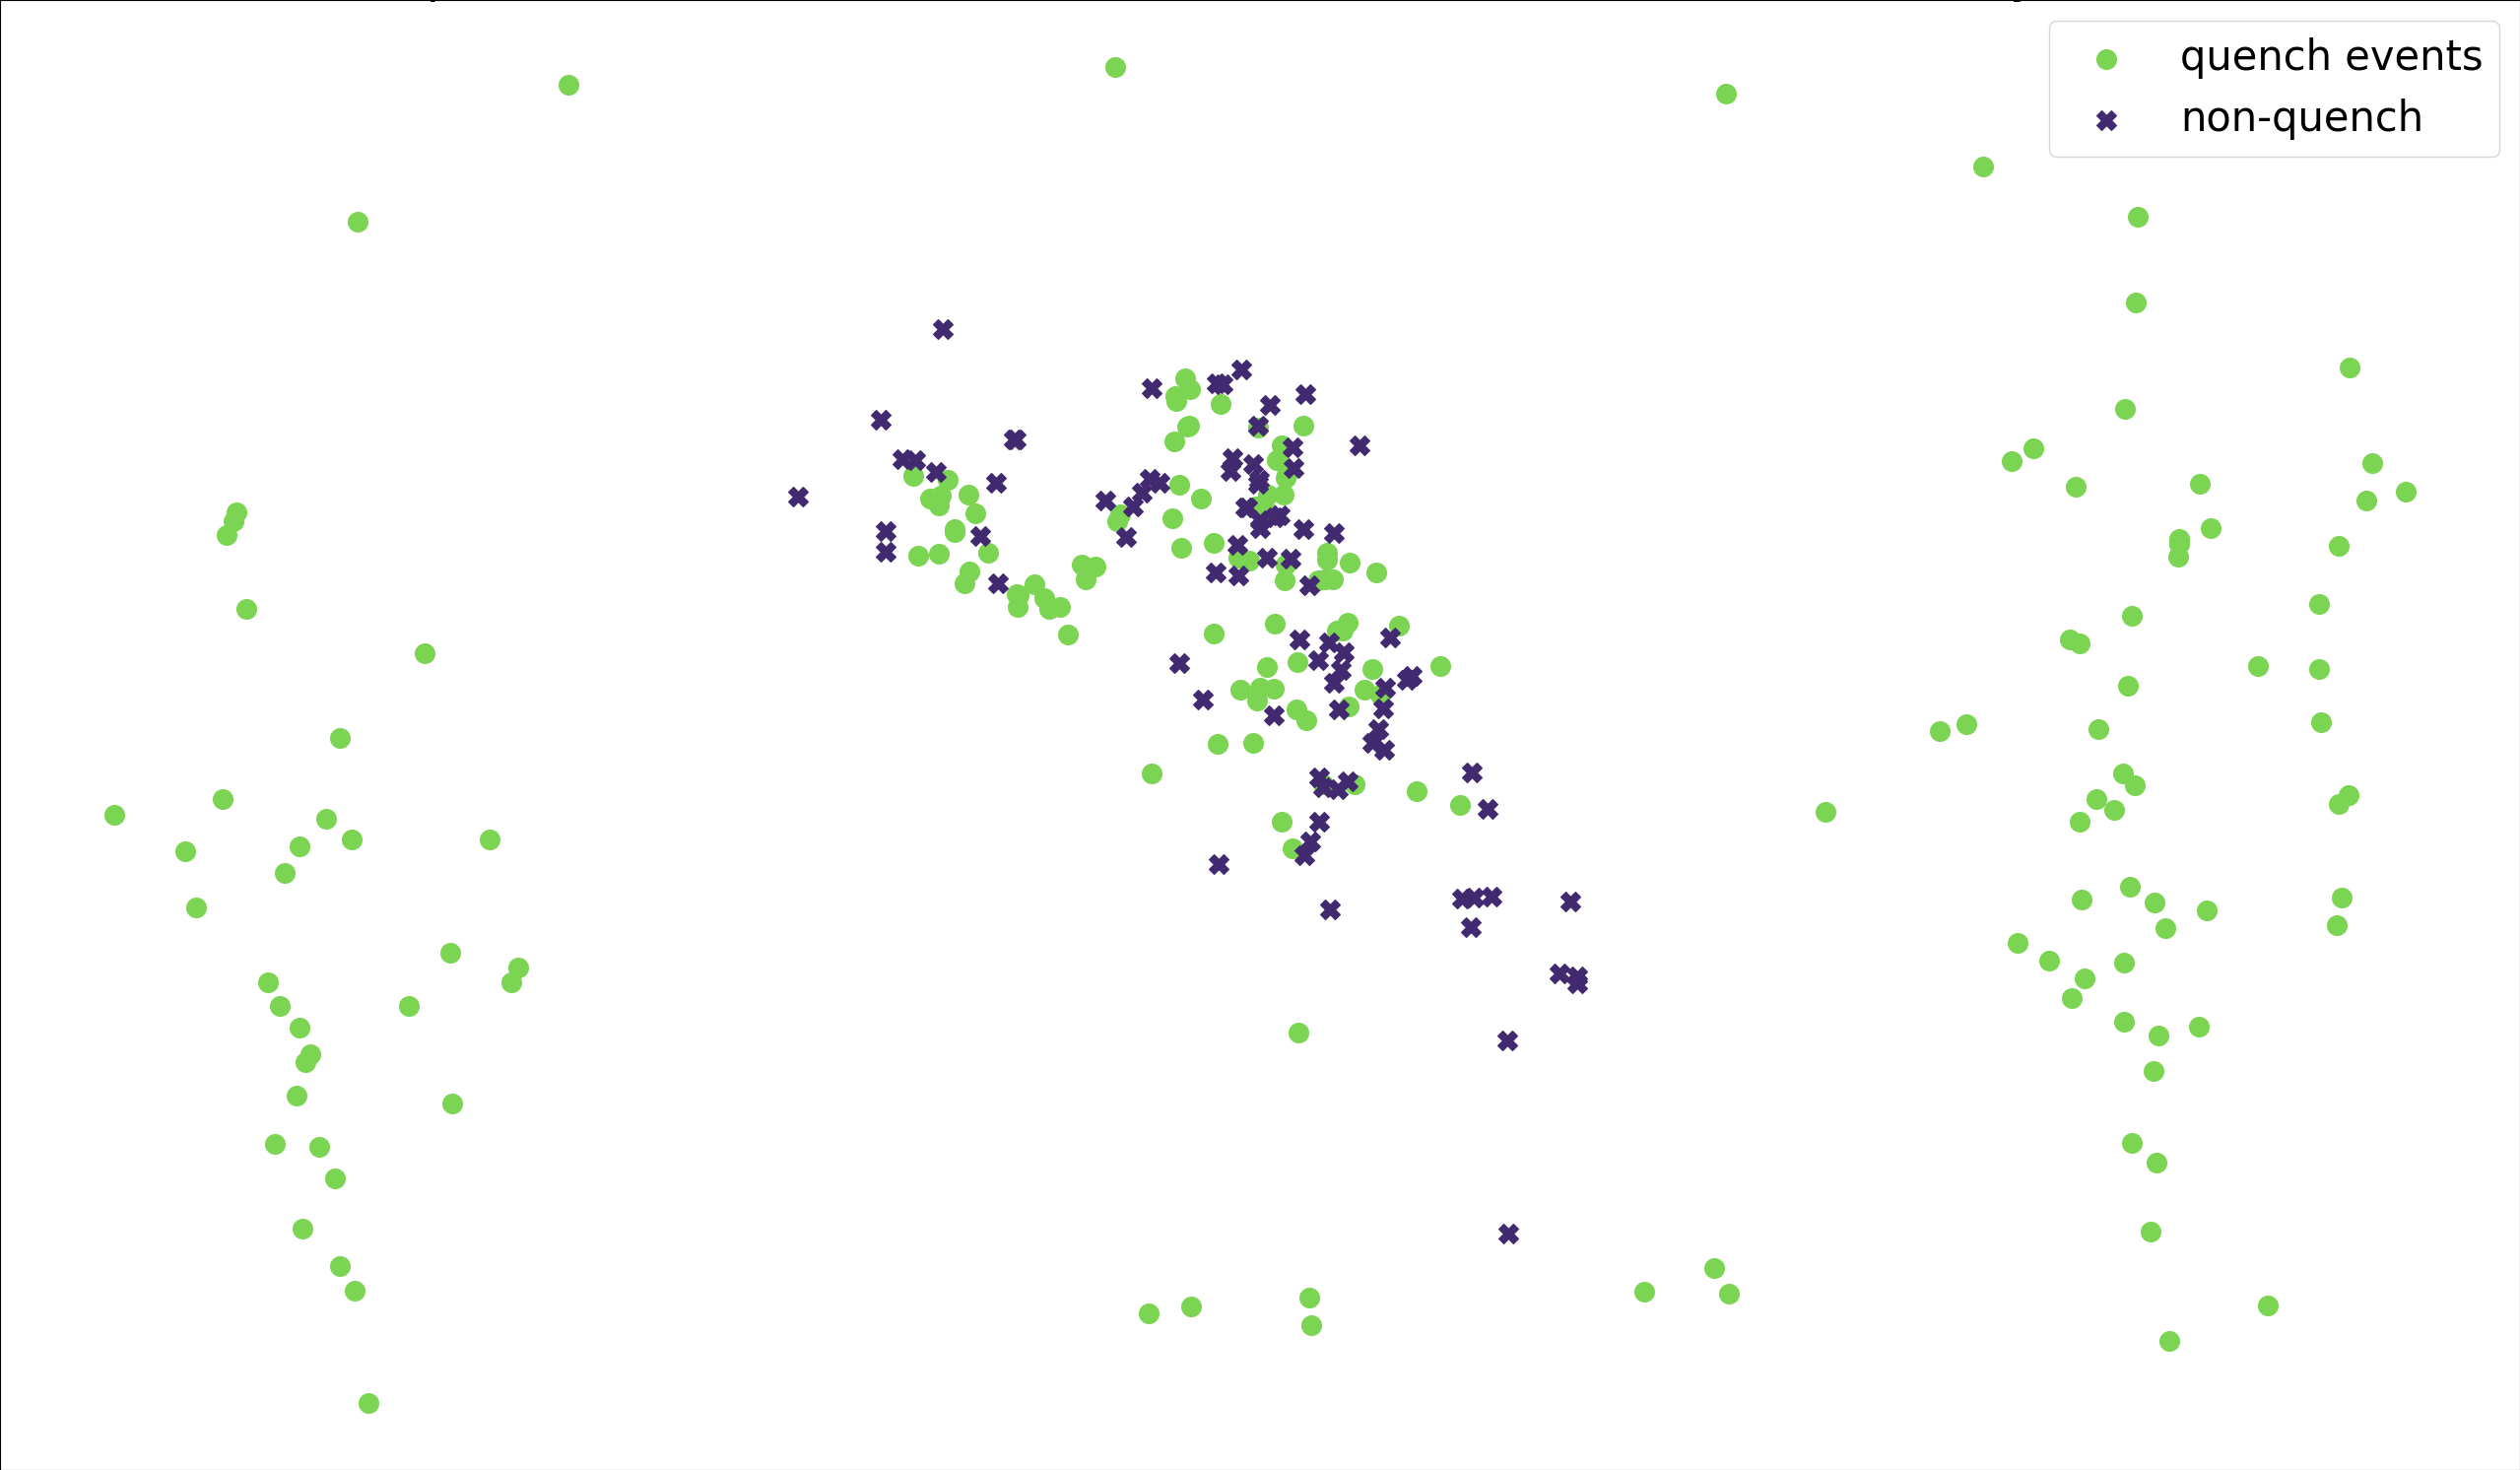
\includegraphics[width=0.7\linewidth]{img/Bn_distribution.png}
	\caption{Data distribution for the \bn\ table after applying \pca\ dimensionality
		reduction, moving from $15$-dimensional space to $2$-dimensional space. In the plot
		we highlight quench and non-quench events.} \label{fig:bn-dist}
\end{figure}

As we did for \an\ we checked the correlation among harmonics for the \bn\ attribute. The results
were very similar, the more striking difference between \Cref{fig:an-corr} and \Cref{fig:bn-corr},
apart from the actual correlation values, is that \bn[2] is not strongly correlated with any other
harmonic (contrarily to \an[2]), while \bn[15] grows a discrete correlation with all odd harmonics.
\begin{figure}[!hb]
	\centering
	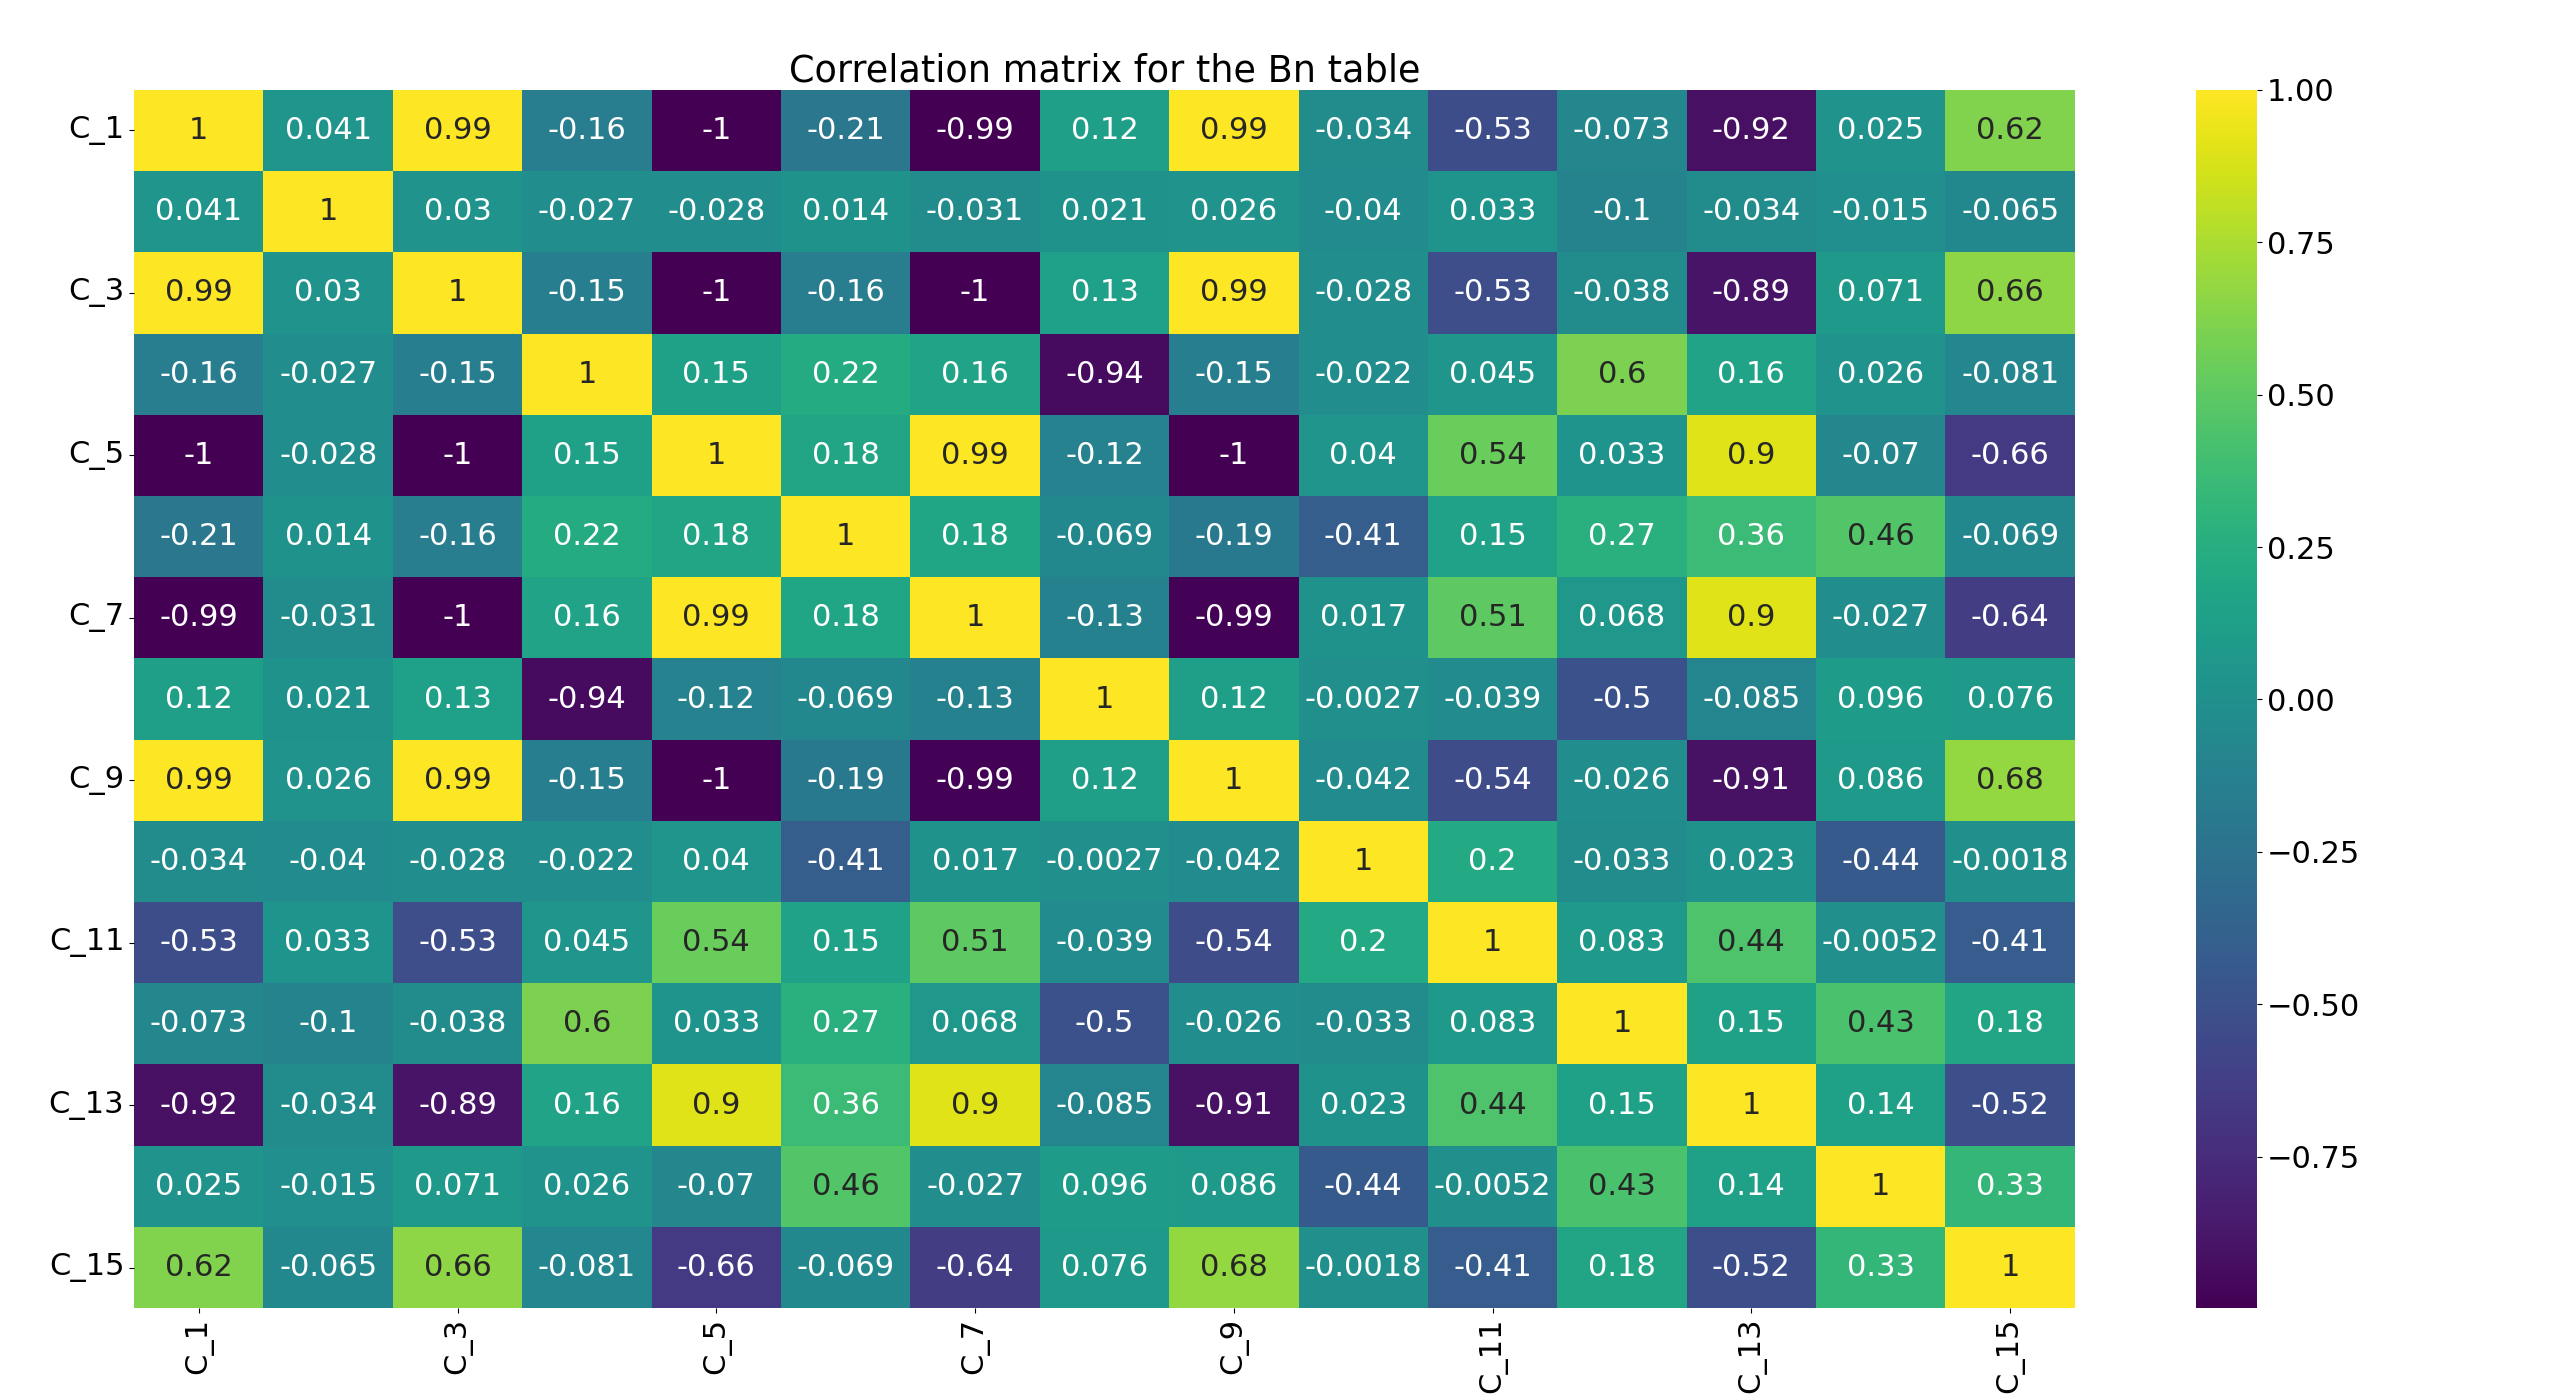
\includegraphics[width=\linewidth]{img/Bn_corr_matrix.png}
	\caption{The cross-correlation among the \bn\ harmonics.} \label{fig:bn-corr}
\end{figure}

If we check the correlation between the harmonics and the labels in (\Cref{fig:bn-lcorr}), we can see
that, apparently, most harmonics have a good enough correlation with the solution, but despite this, the performance of all
models built on \bn\ suffered. As we will see in \Cref{sec:results-qrp}, independently of the sub-view chosen for \bn, the model
performance was always lagging behind the alternatives. This attribute was mainly useful as an extra
source of information (see \Cref{sec:qrp-ta}) or to build training datasets for models capable of
gathering more information from the data, like \rfs (see \Cref{sec:qrp-rf}).
\begin{figure}[!hb]
	\centering
	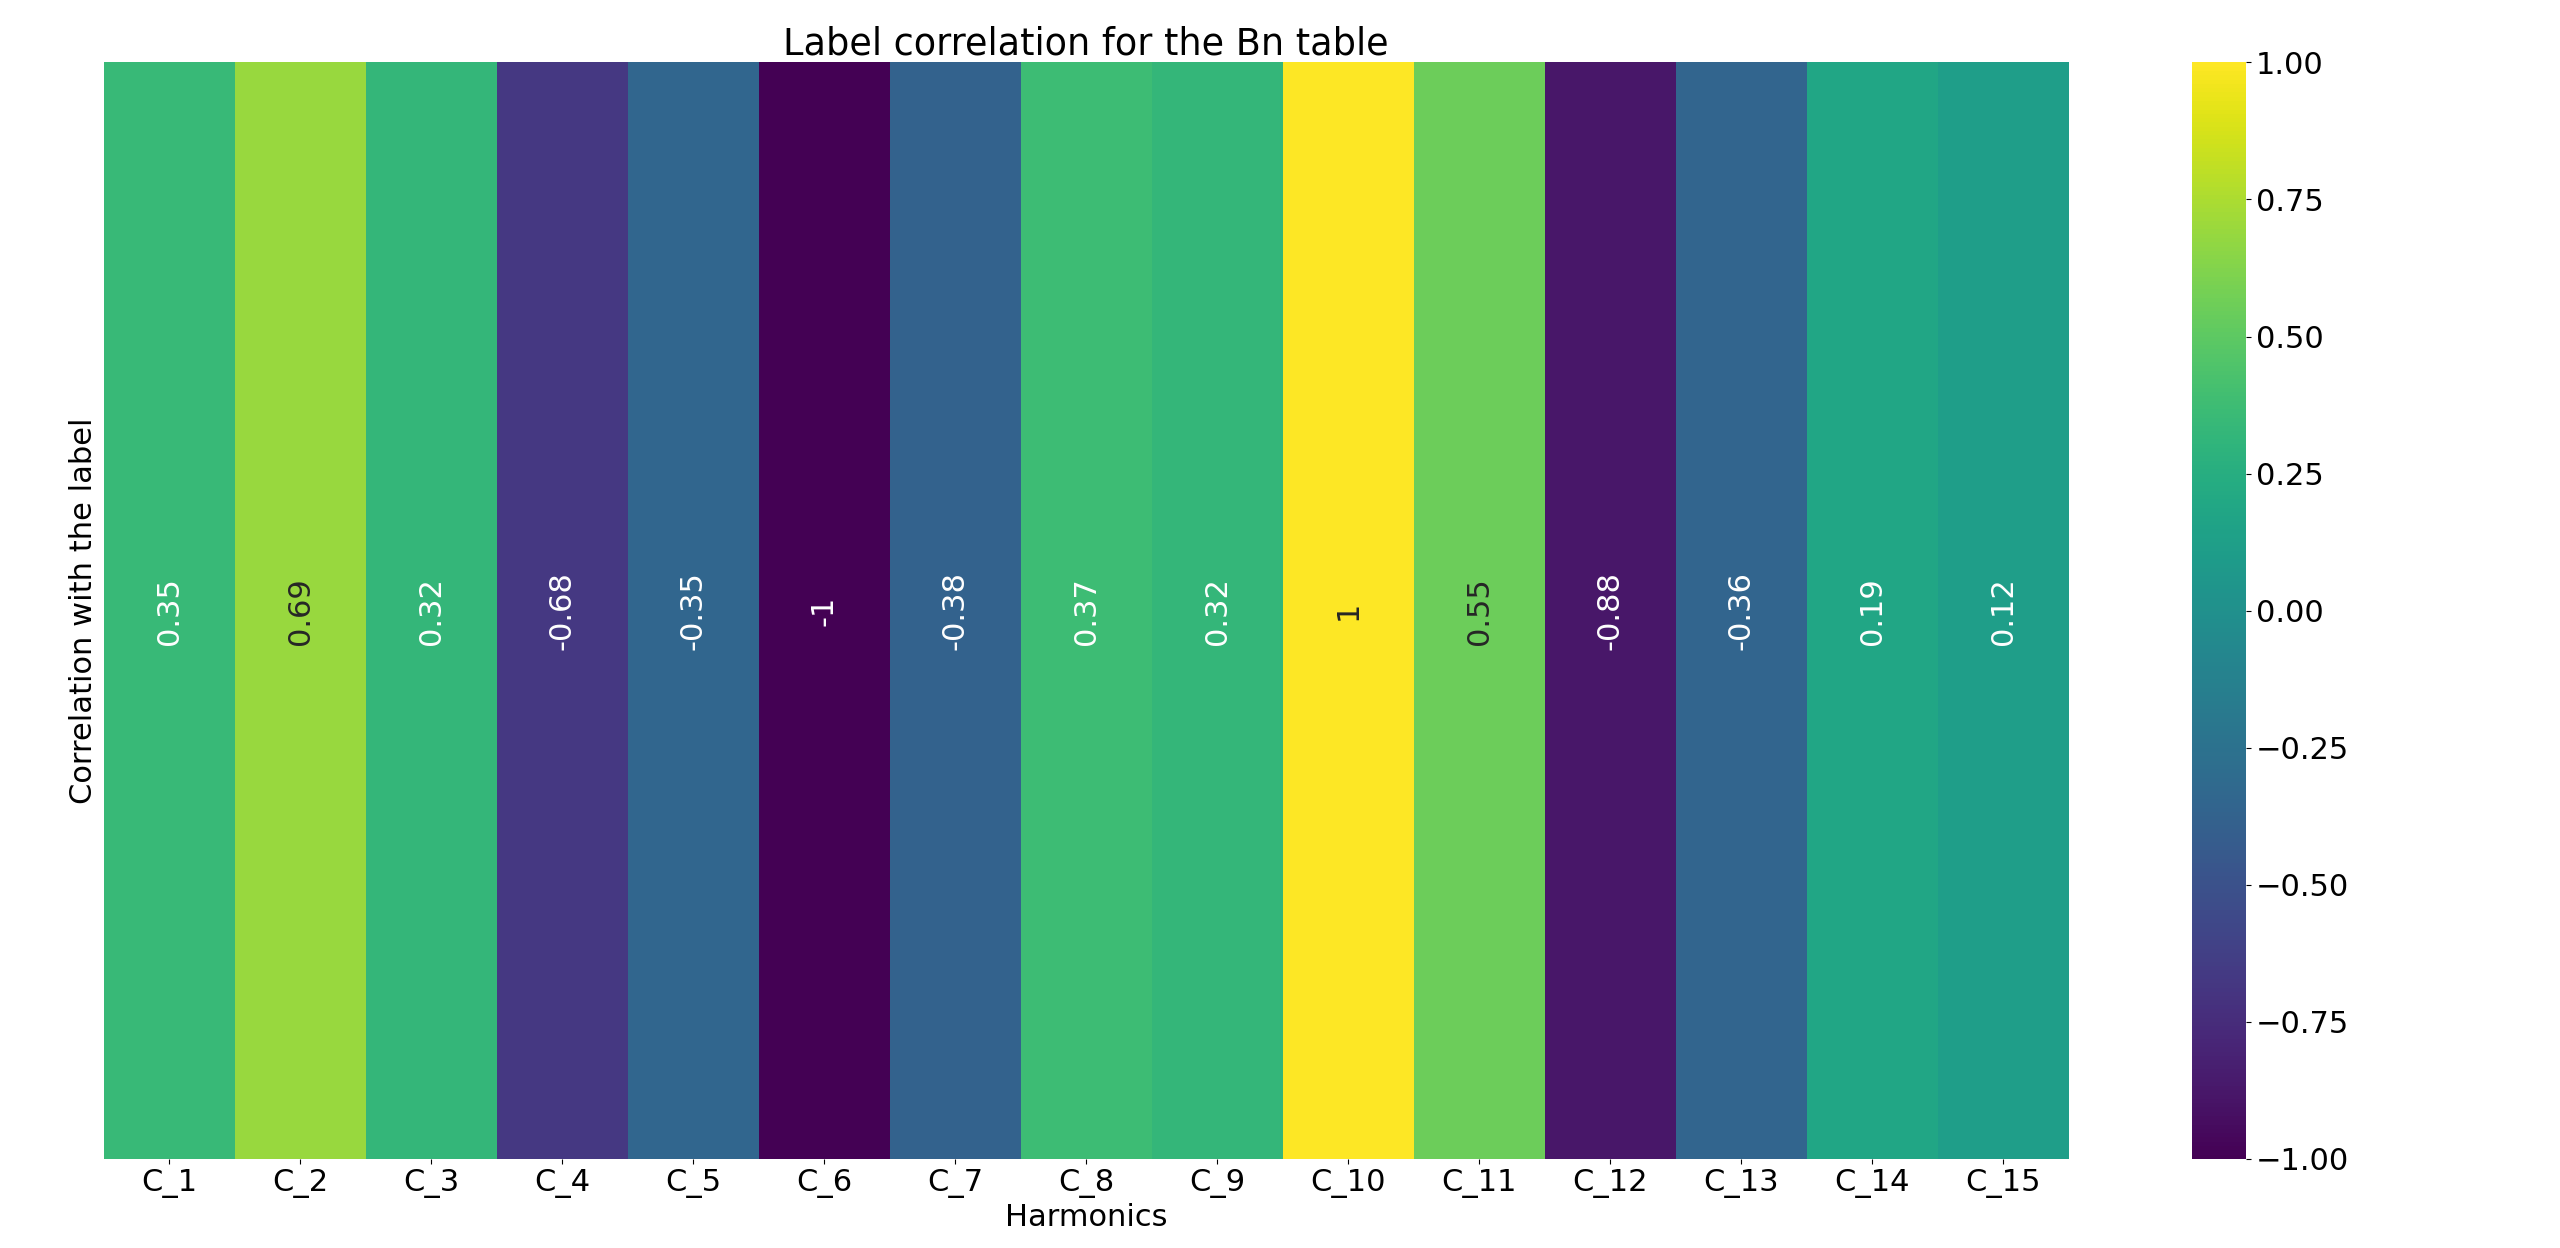
\includegraphics[width=0.7\linewidth]{img/Bn_label_corr.png}
	\caption{Correlation between the harmonics and the labels for \bn.} \label{fig:bn-lcorr}
\end{figure}

\subsubsection{\cnmod}
The \cnmod\ attribute combines the information present in \an\ and \bn. \cnmod\ was expected to be one
of the best attributes to solve \qrp, as we highlighted in \Cref{chp:problem}; as we will see in
future sections, while models trained on \cnmod\ cannot reach the same level of performance obtained
by training on \an, they are consistently the second-best model available.
\begin{figure}[!ht]
	\centering
	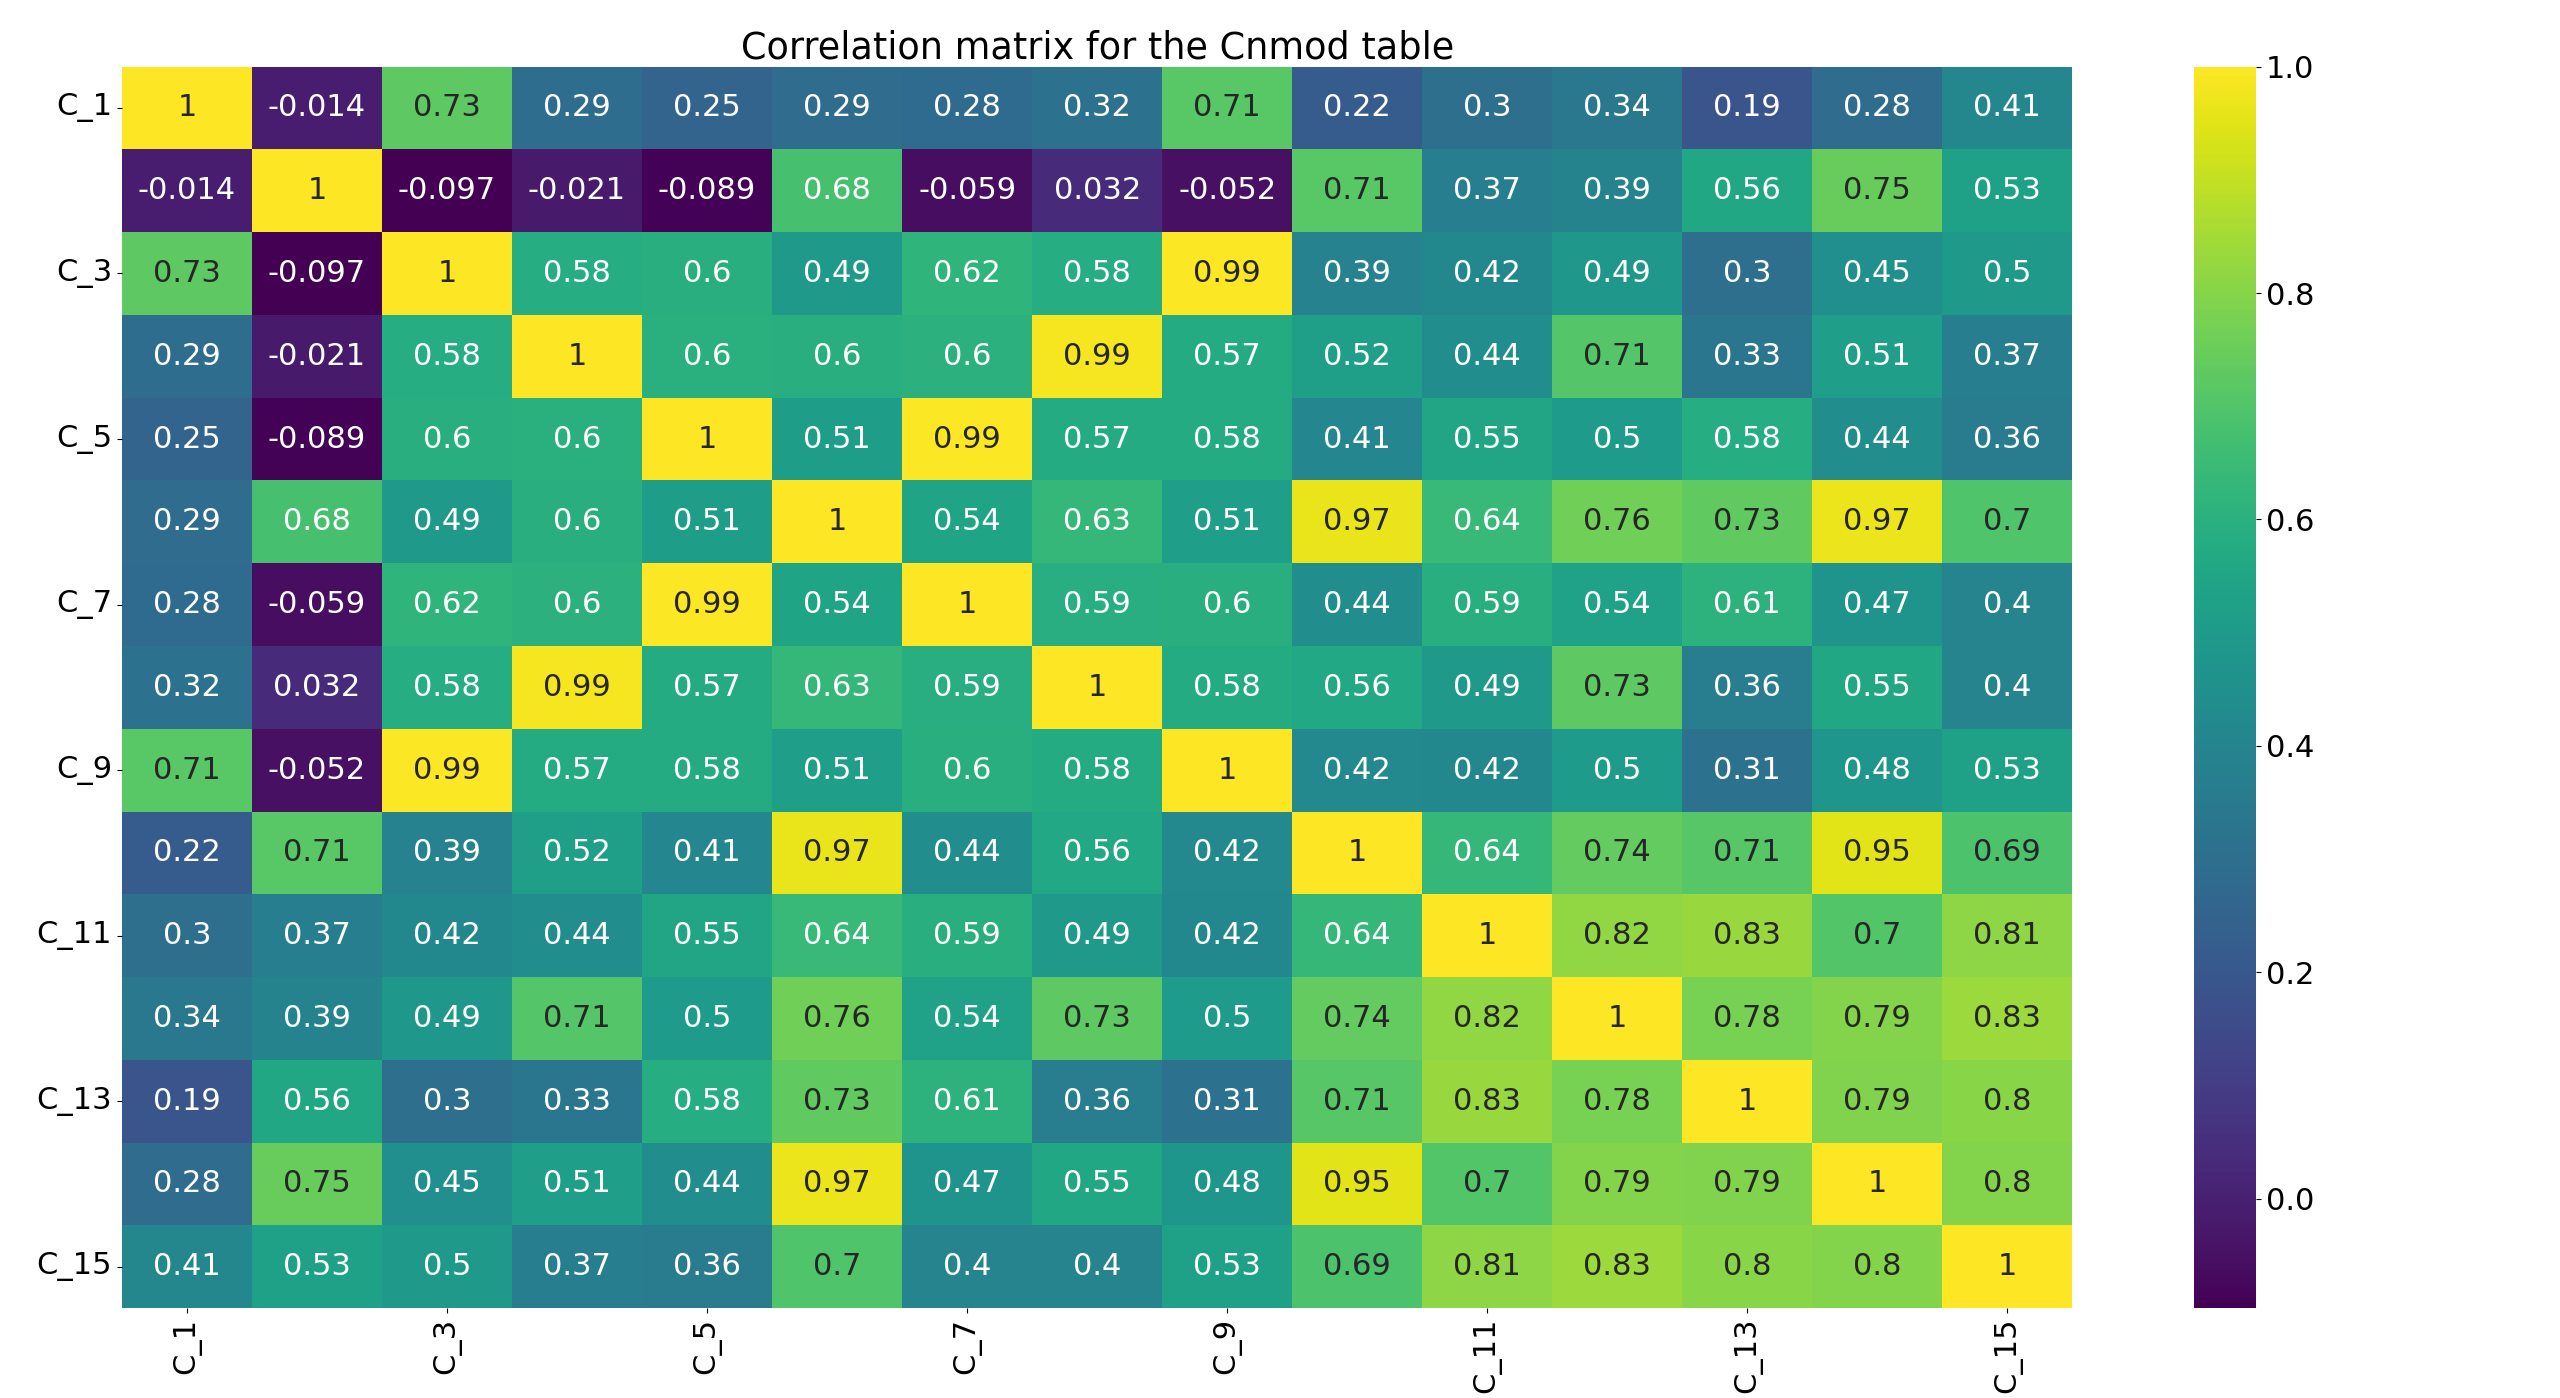
\includegraphics[width=\linewidth]{img/Cnmod_corr_matrix.png}
	\caption{The cross-correlation among the \cnmod\ harmonics.} \label{fig:cnmod-corr}
\end{figure}

\Cref{fig:cnmod-corr} shows the correlation matrix for \cnmod, its structure is very complicated,
since:
\begin{itemize}
	\item \cnmod[2] is strongly correlated with all harmonics until \cnmod[9],
	\item Harmonics between \cnmod[10] and \cnmod[15] are strongly correlated among themselves,
	\item \cnmod[4] is strongly correlated with its multiples.
\end{itemize}
\begin{figure}[!ht]
	\centering
	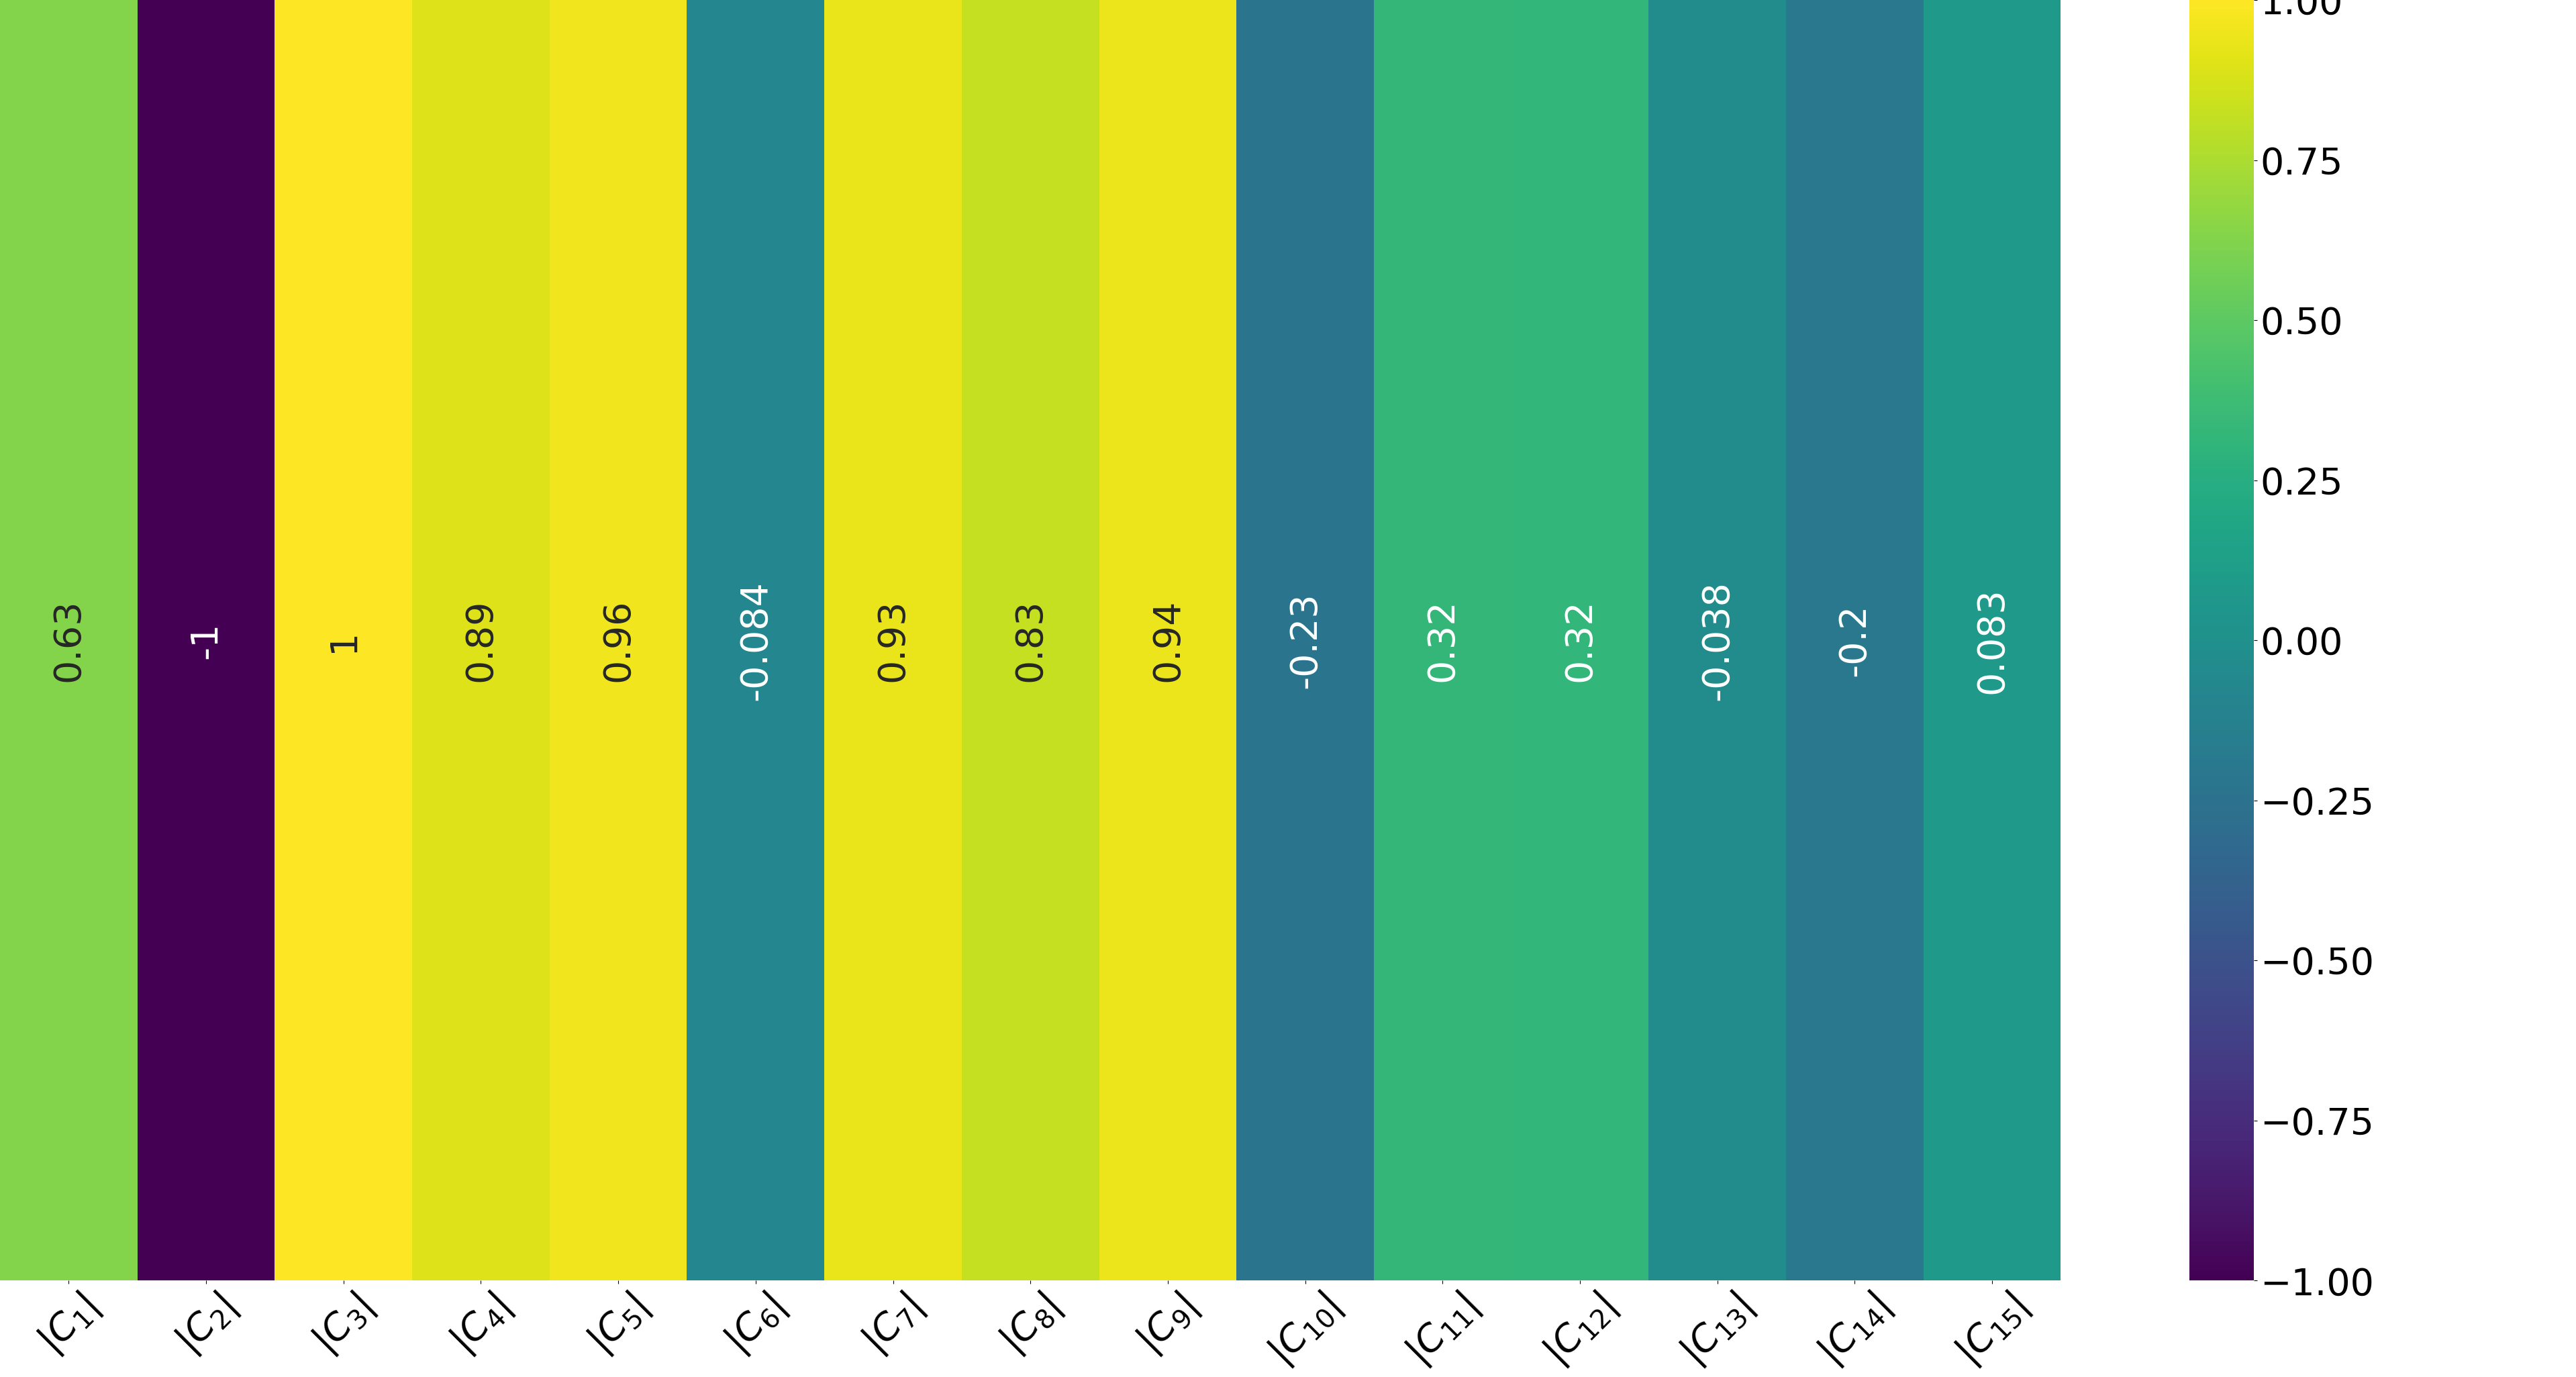
\includegraphics[width=0.7\linewidth]{img/Cnmod_label_corr.png}
	\caption{Correlation between the harmonics and the labels for \cnmod.} \label{fig:cnmod-lcorr}
\end{figure}

Looking at both \Cref{fig:cnmod-corr} and \Cref{fig:cnmod-lcorr}, we can conclude that two different
approaches can be followed:
\begin{itemize}
	\item Using \cnmod[2] alongside one or more high-order harmonics,
	\item Using \cnmod[3] and some other low-order harmonics (potentially even the
	      first one) alongside one high-order harmonic (e.g., \cnmod[14]).
\end{itemize}
Analyzing the box-plot suggested that using harmonic number \cnmod[2] was not promising, due to the extreme
concentration of the data. Furthermore, during testing (see \Cref{sec:qrp-dt}), we obtained more
promising results for trees using a sub-view centered around harmonic $2$, but when it came to
ensemble learning the better alternative revealed to be a sub-view centered around harmonic $3$.

\medskip

\Cref{fig:cnmod-dist} visualizes the distribution of the samples in \cnmod\ after a round of \pca,
the samples are characterized by a good enough distribution, we could easily identify clusters with
a high degree of purity, apart from the one in the leftmost region of the image, which contains
samples belonging to both classes mixed together homoegeneously. In the rightmost part of the image
there is an outlier that has been removed when we began working with $k$-means. Overall \cnmod\
doesn't have a distribution quite as good as \an\ did, but comparing it to \Cref{fig:bn-dist} or
\phin bidimensional visualization (see \Cref{fig:phi-dist}), it has a much better topology.
\begin{figure}[!ht]
	\centering
	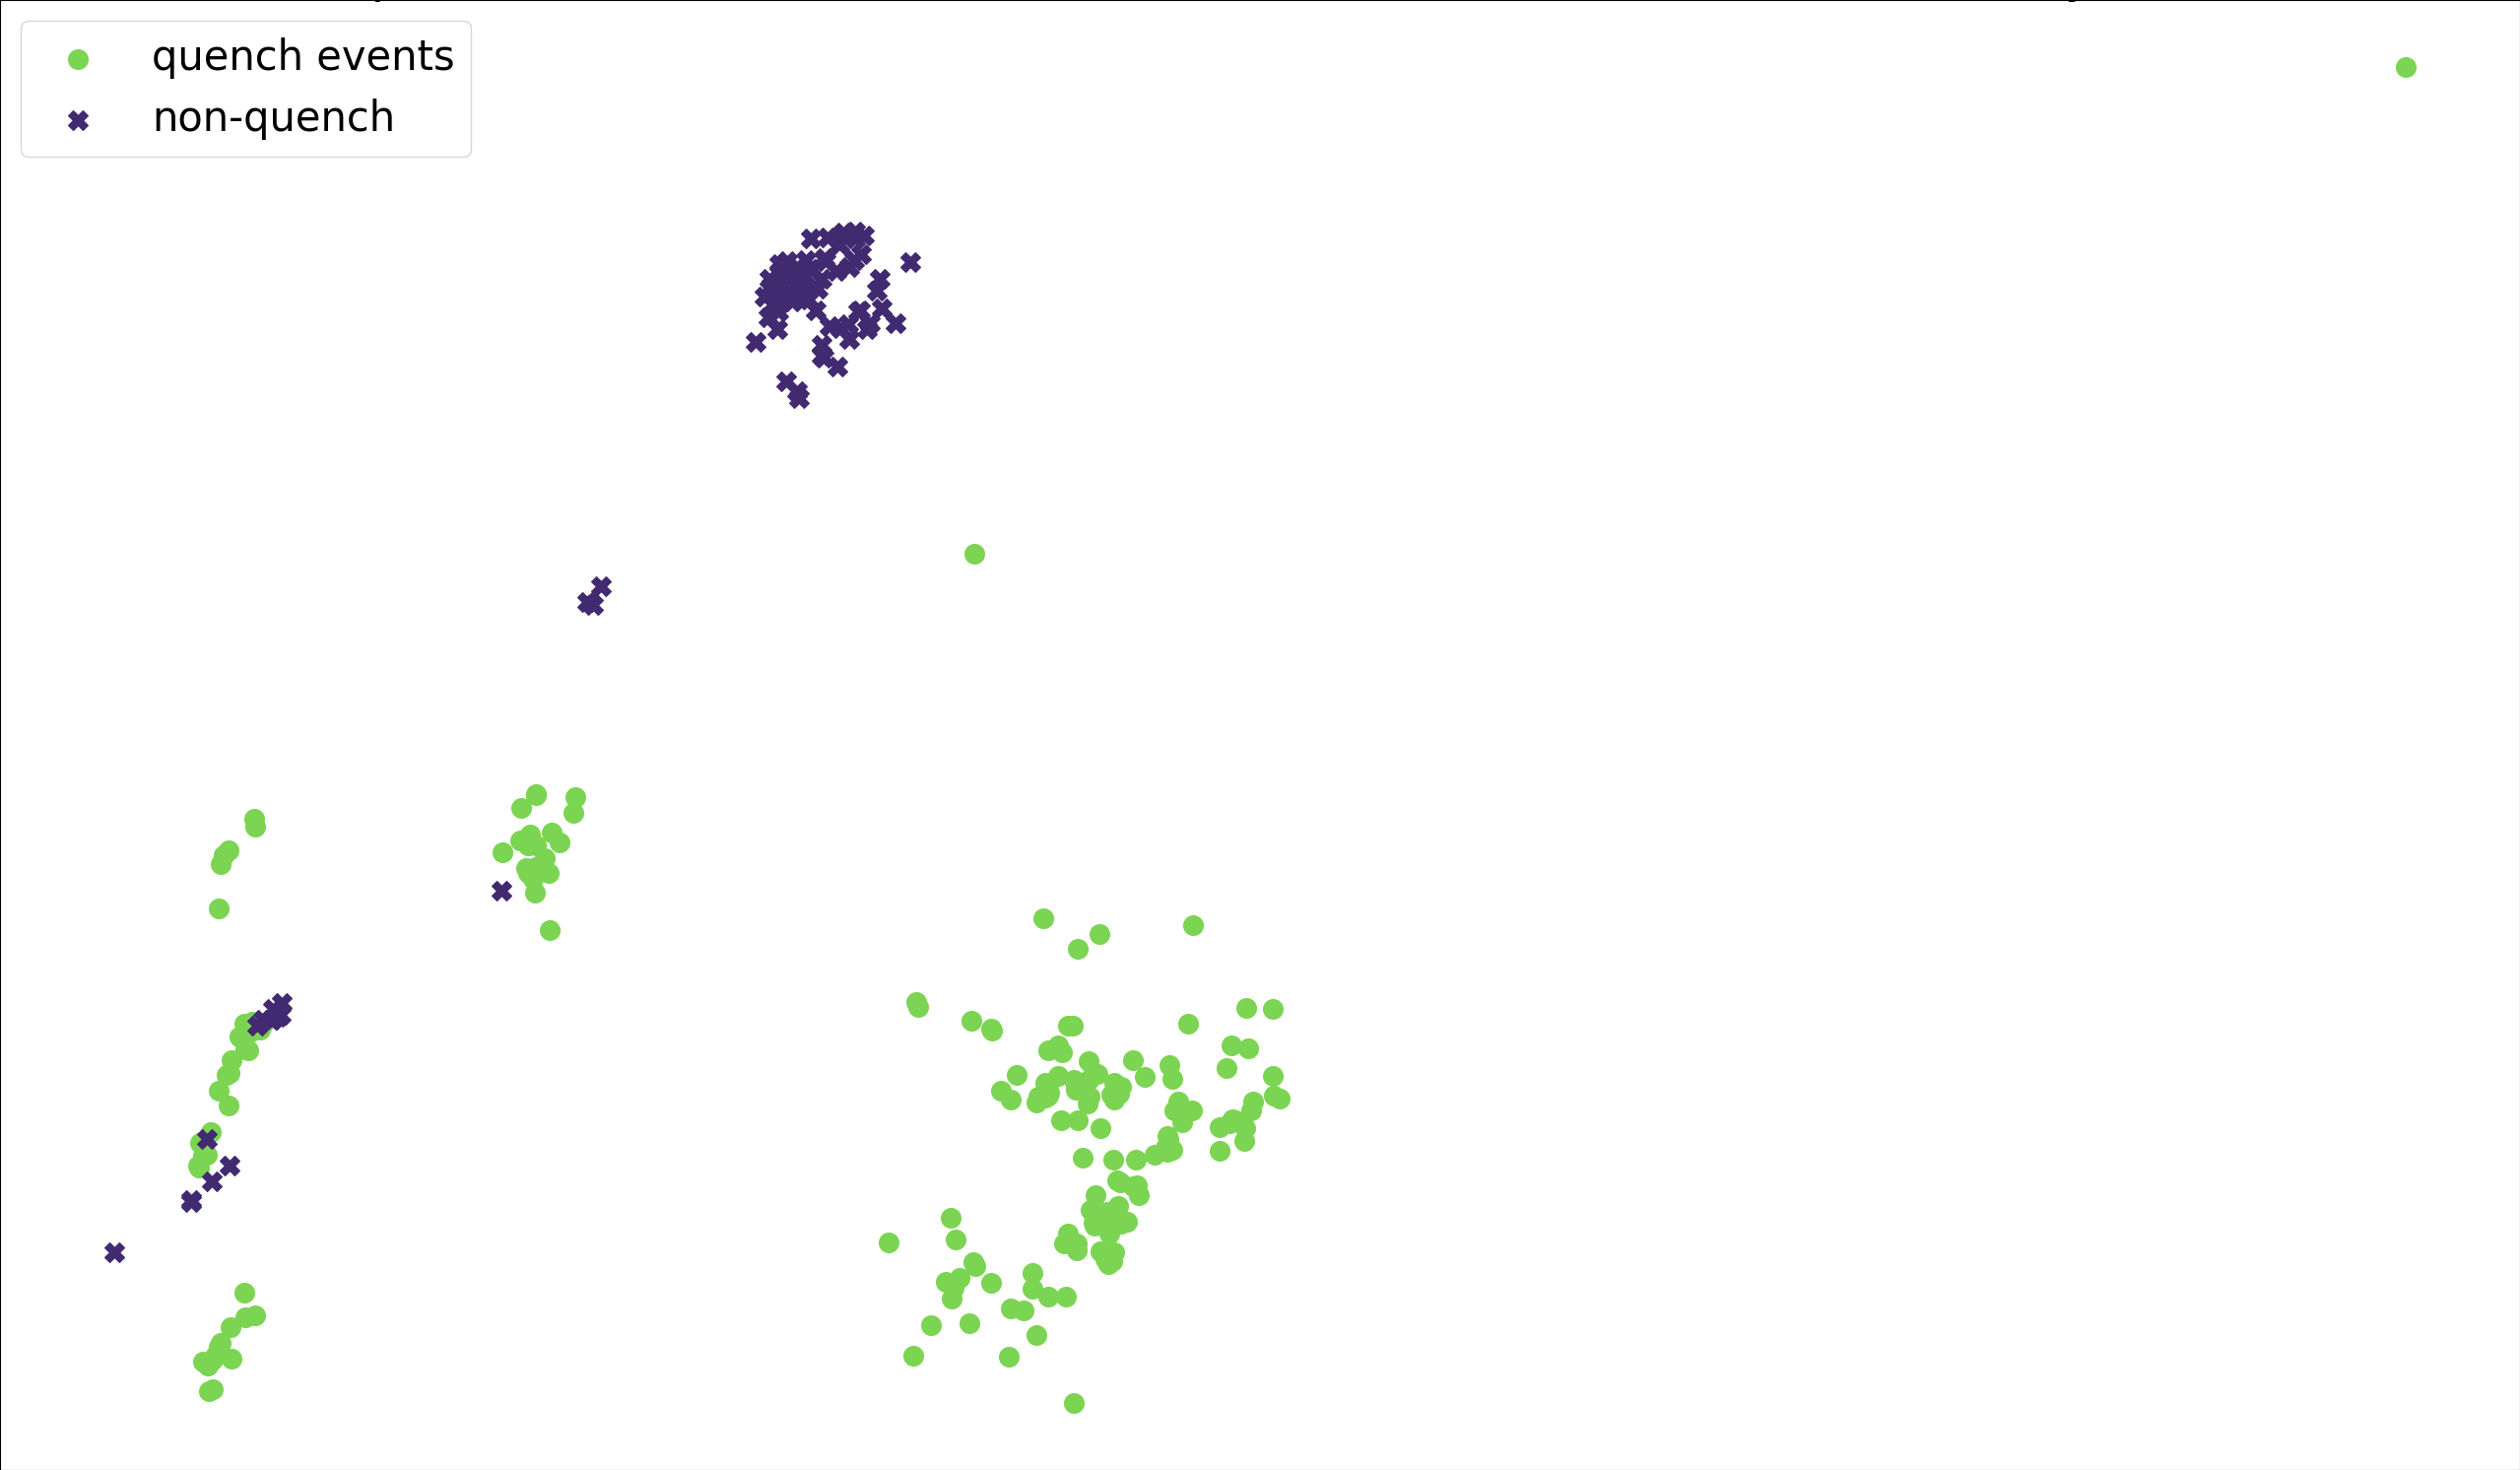
\includegraphics[width=0.7\linewidth]{img/Cnmod_distribution.png}
	\caption{Data distribution for the \cnmod\ table after applying \pca\ dimensionality
		reduction, moving from $15$-dimensional space to $2$-dimensional space-dimensional
		space. In the plot we highlight quench and non-quench events.} \label{fig:cnmod-dist}
\end{figure}

\subsubsection{\phin}
As we will see in further sections the \phin-based models consistently outperformed the ones based
on \bn. \phin, as in the case of \bn, has a very homogeneous bidimensional visualization, as shown in
\Cref{fig:phi-dist}, containing a series of high-impurity clusters, where samples of the two classes are mixed together.
\begin{figure}[!ht]
	\centering
	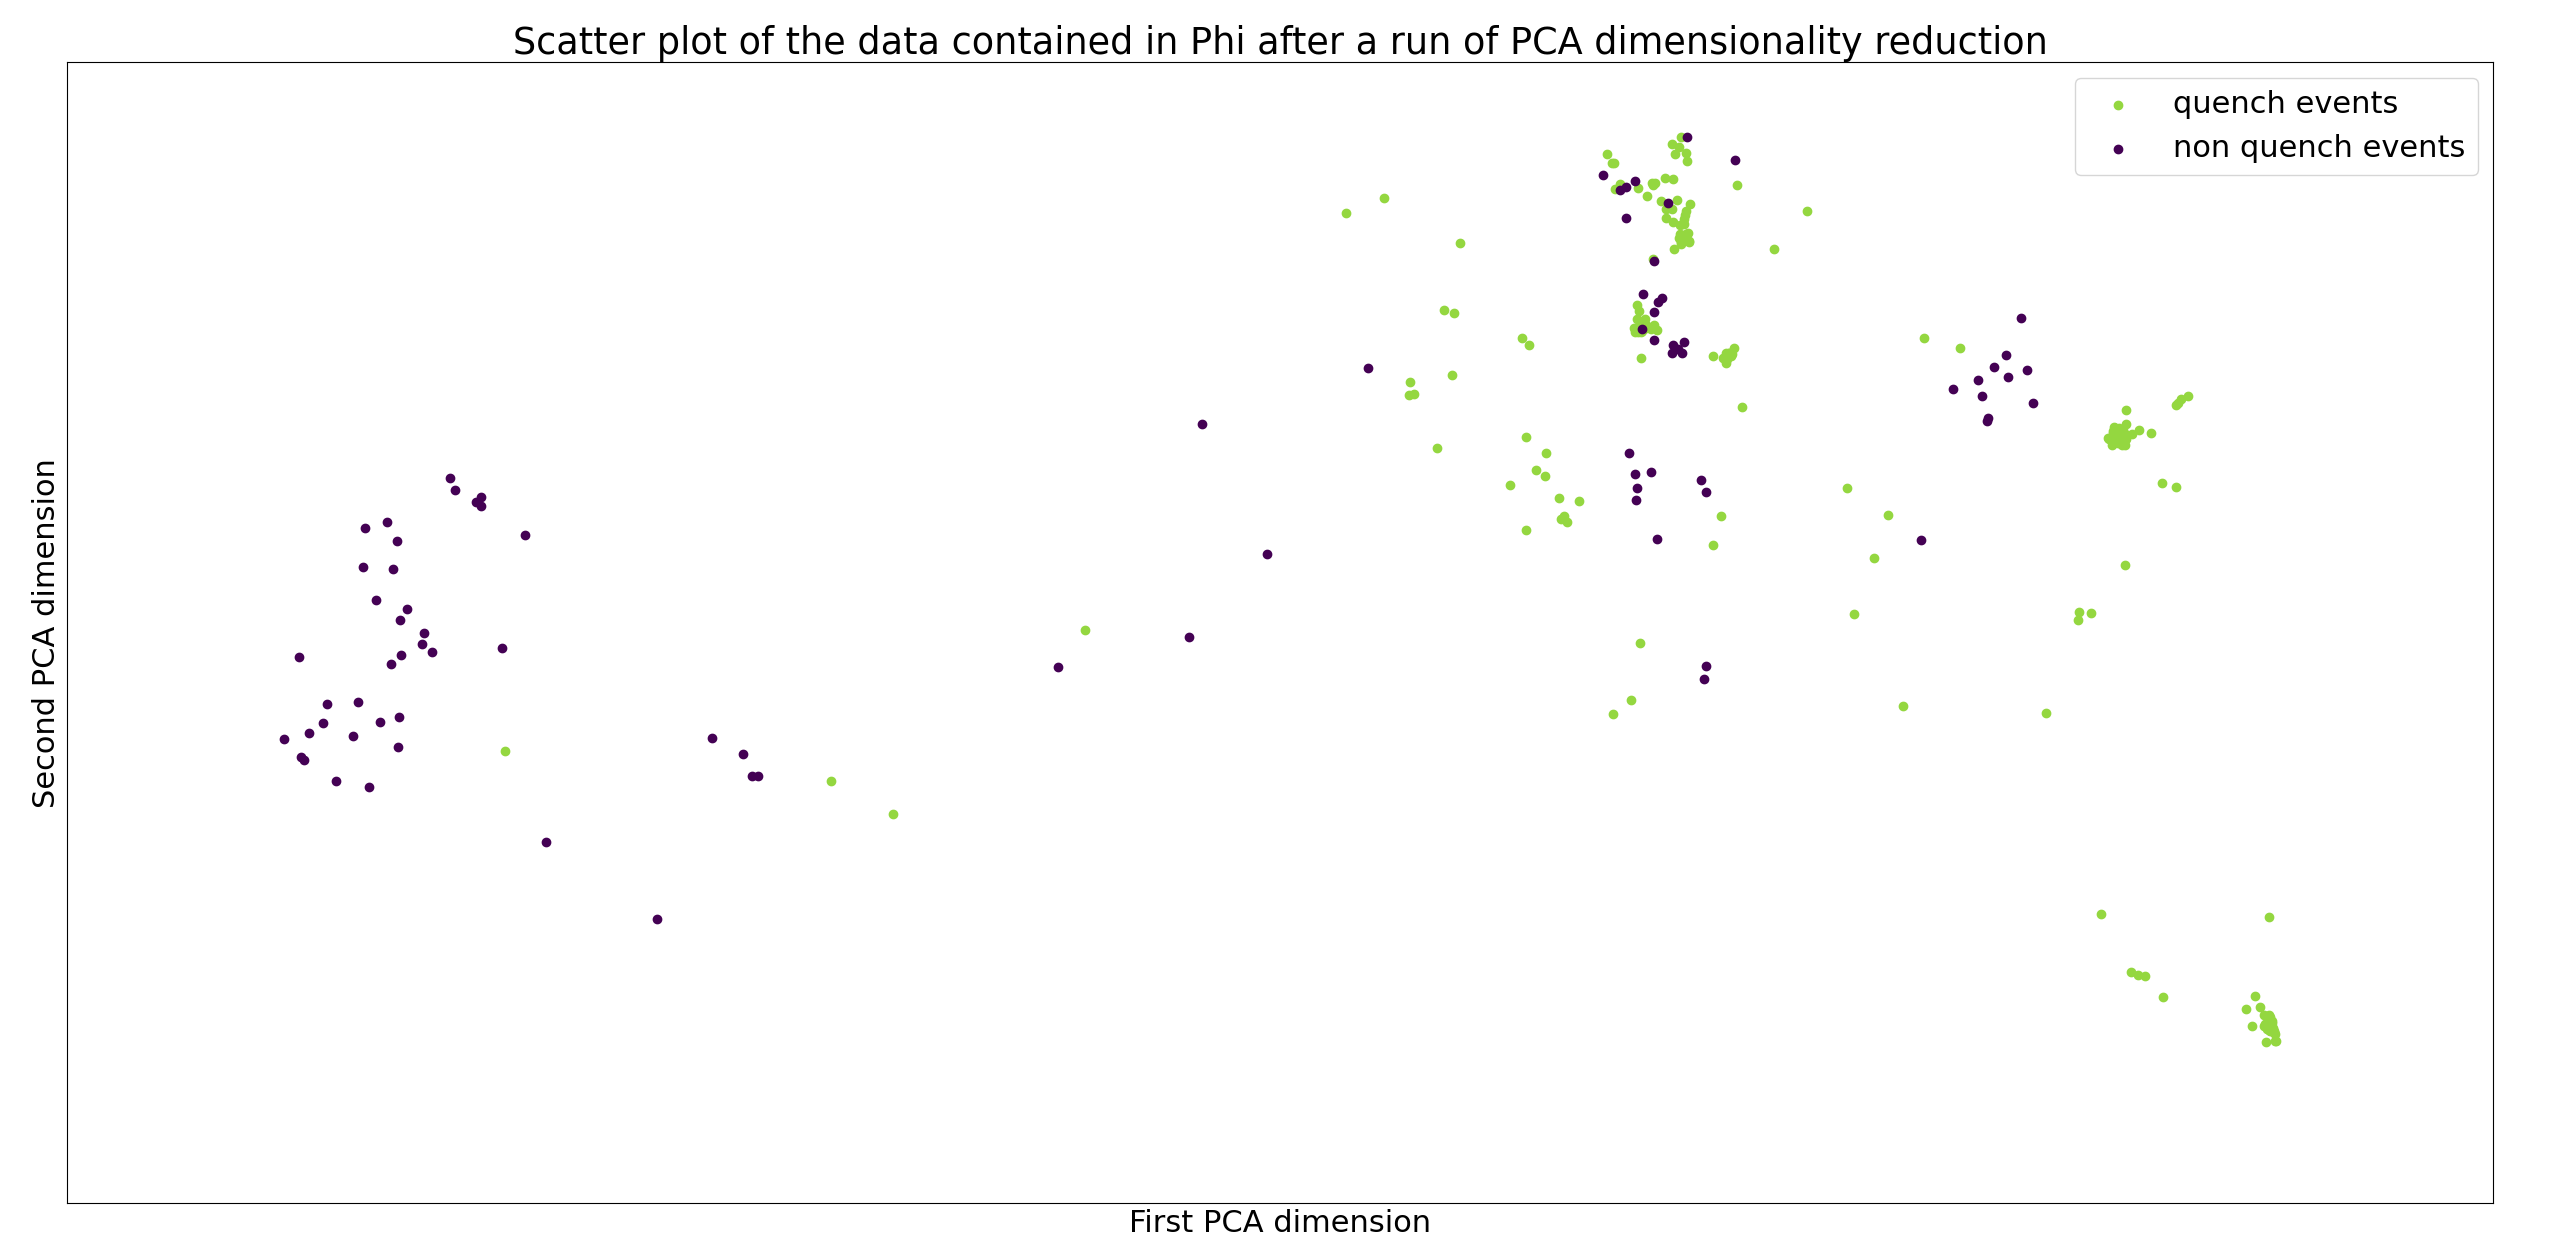
\includegraphics[width=0.7\linewidth]{img/Phi_distribution.png}
	\caption{Data distribution for the \phin\ table after applying \pca\ dimensionality
		reduction, moving from $15$-dimensional space to $2$-dimensional space-dimensional
		space. In the plot we highlight quench and non-quench events.} \label{fig:phi-dist}
\end{figure}

In \Cref{fig:phi-corr} we plotted the correlation matrix for \phin, contrarily to the correlation
matrix of other attributes, the amount of harmonics that are strongly correlated with each other is very
low, only: \phin[2] and its odd multiples and \phin[4] and its multiples are strongly correlated. Compared to the
aforementioned attributes the matrix contains no real structure, which leaves us freedom to choose
whichever harmonics are better to train our models.
\begin{figure}[!ht]
	\centering
	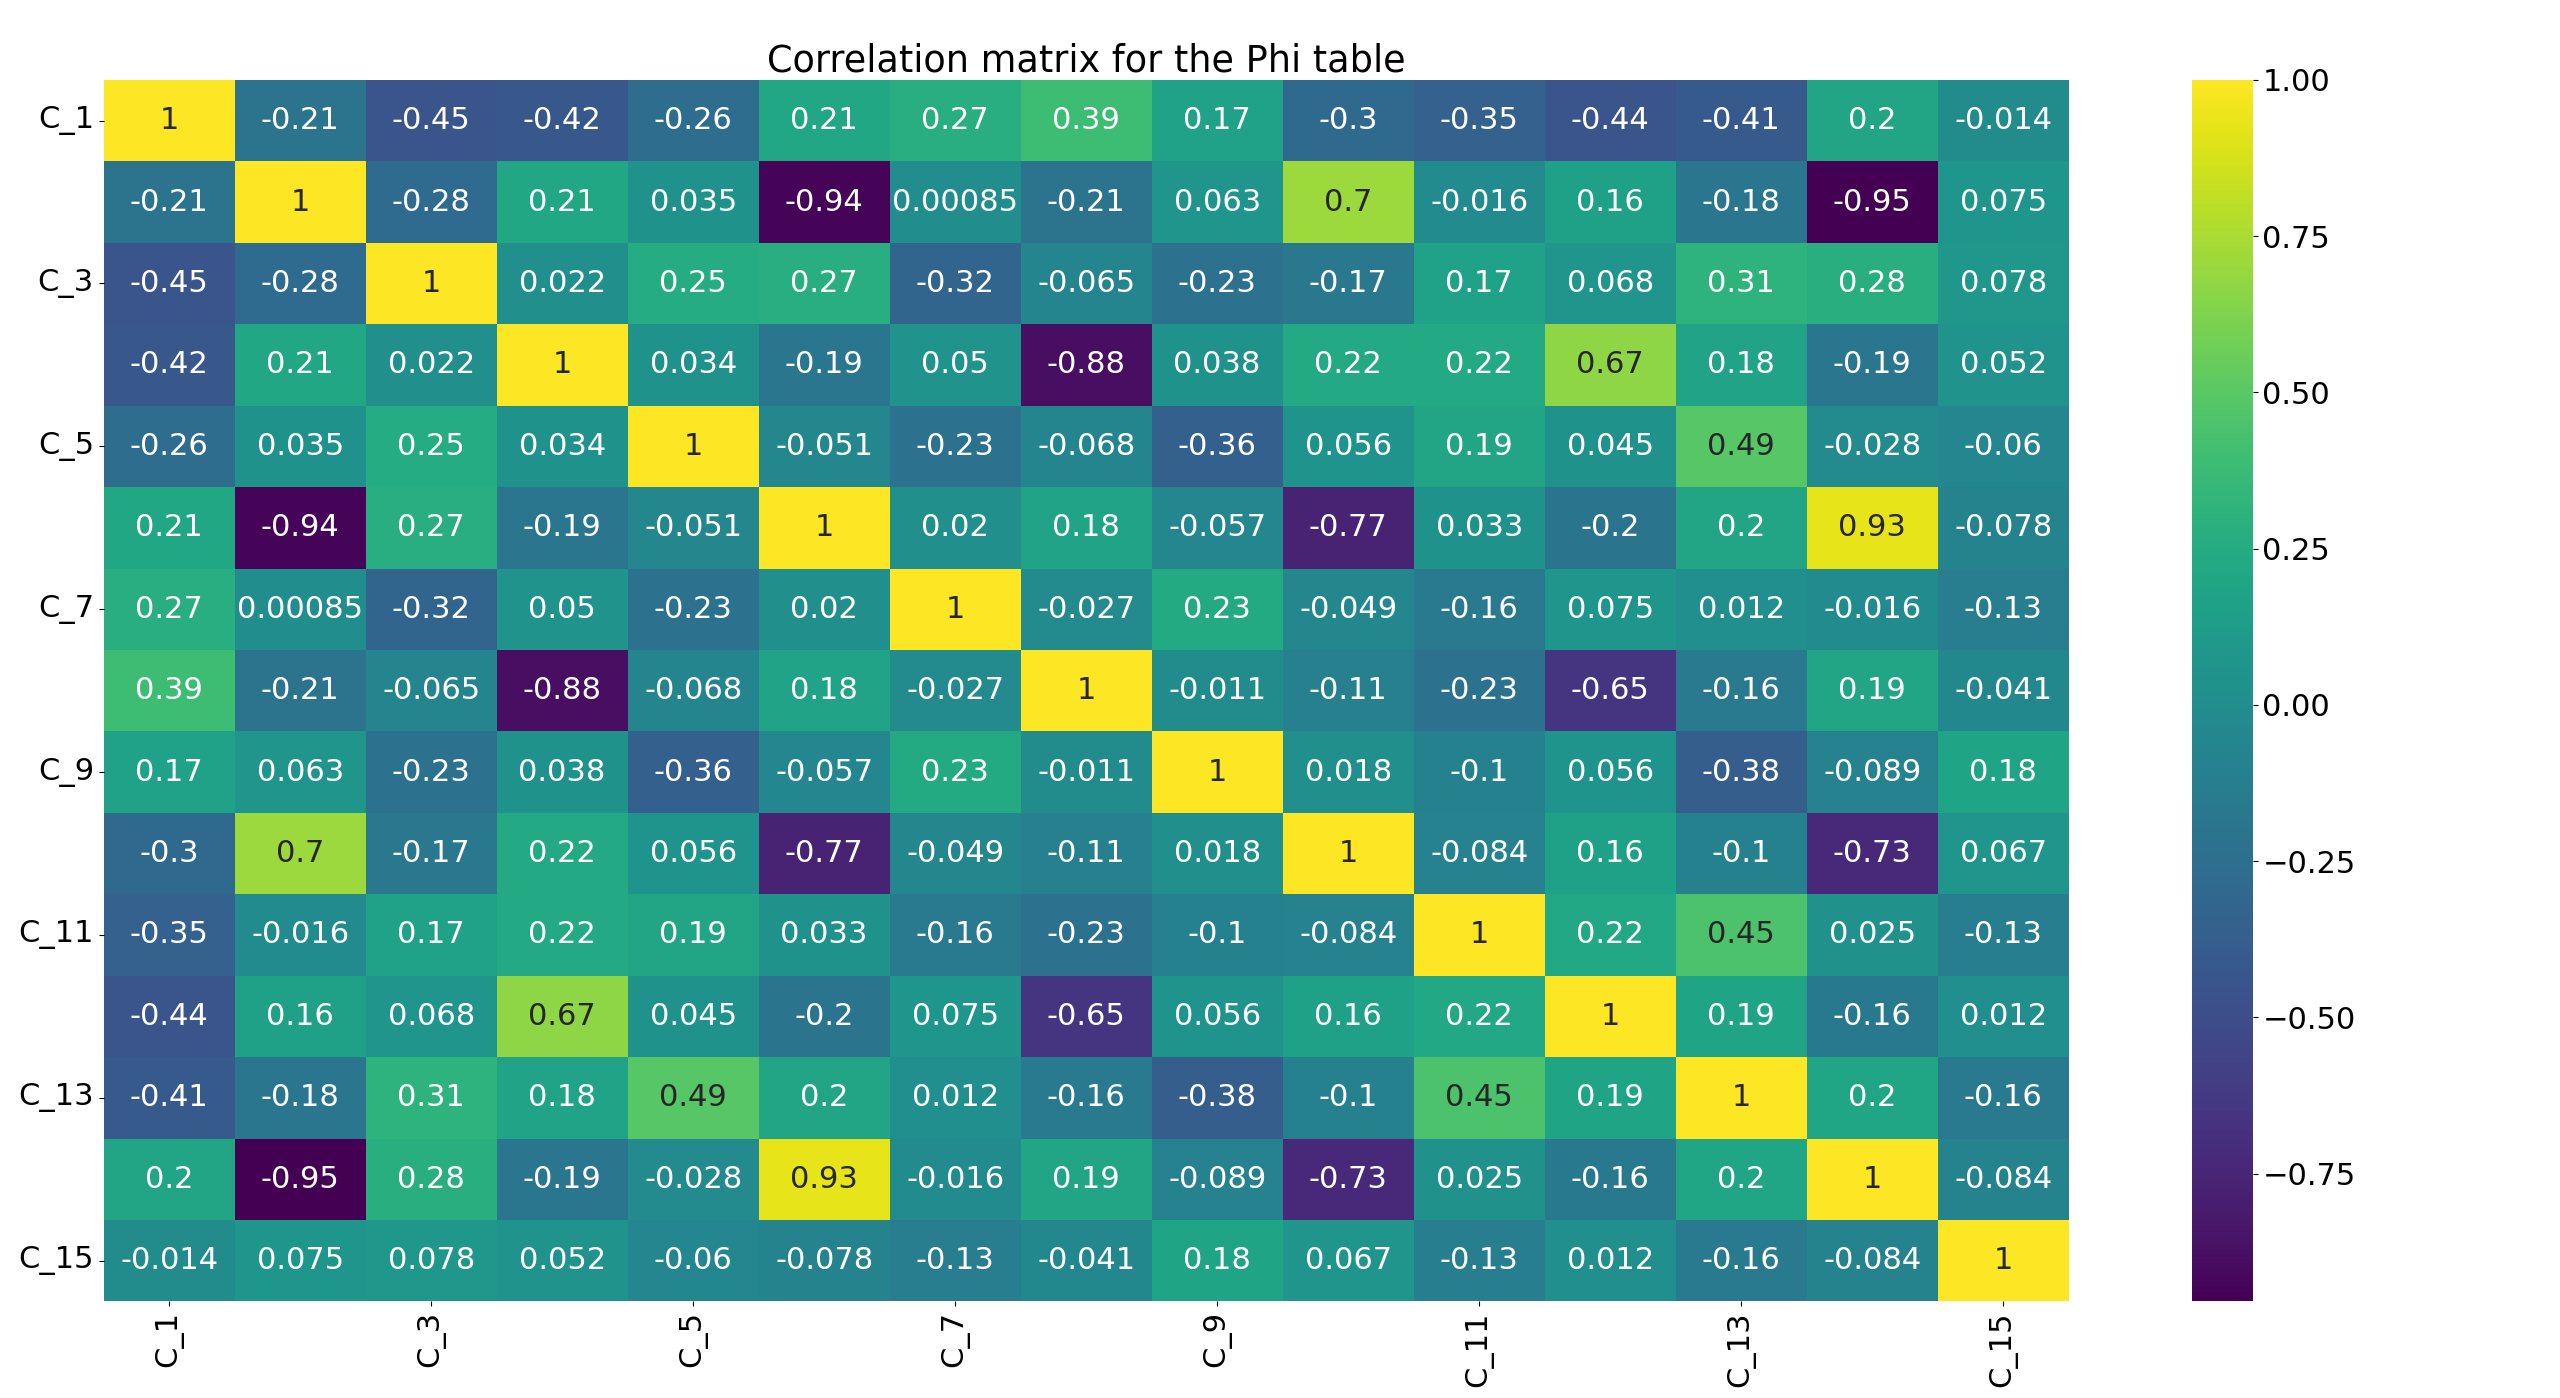
\includegraphics[width=\linewidth]{img/Phi_corr_matrix.png}
	\caption{The cross-correlation among the \phin\ harmonics.} \label{fig:phi-corr}
\end{figure}

Lastly, we can analyze the correlation between the harmonics and the labels. As we can see in
\Cref{fig:phi-lcorr} most of the harmonics have a good correlation with the expected solution,
especially \phin[2]\ and its odd multiples, \phin[1]\ and \phin[12].
\begin{figure}[!ht]
	\centering
	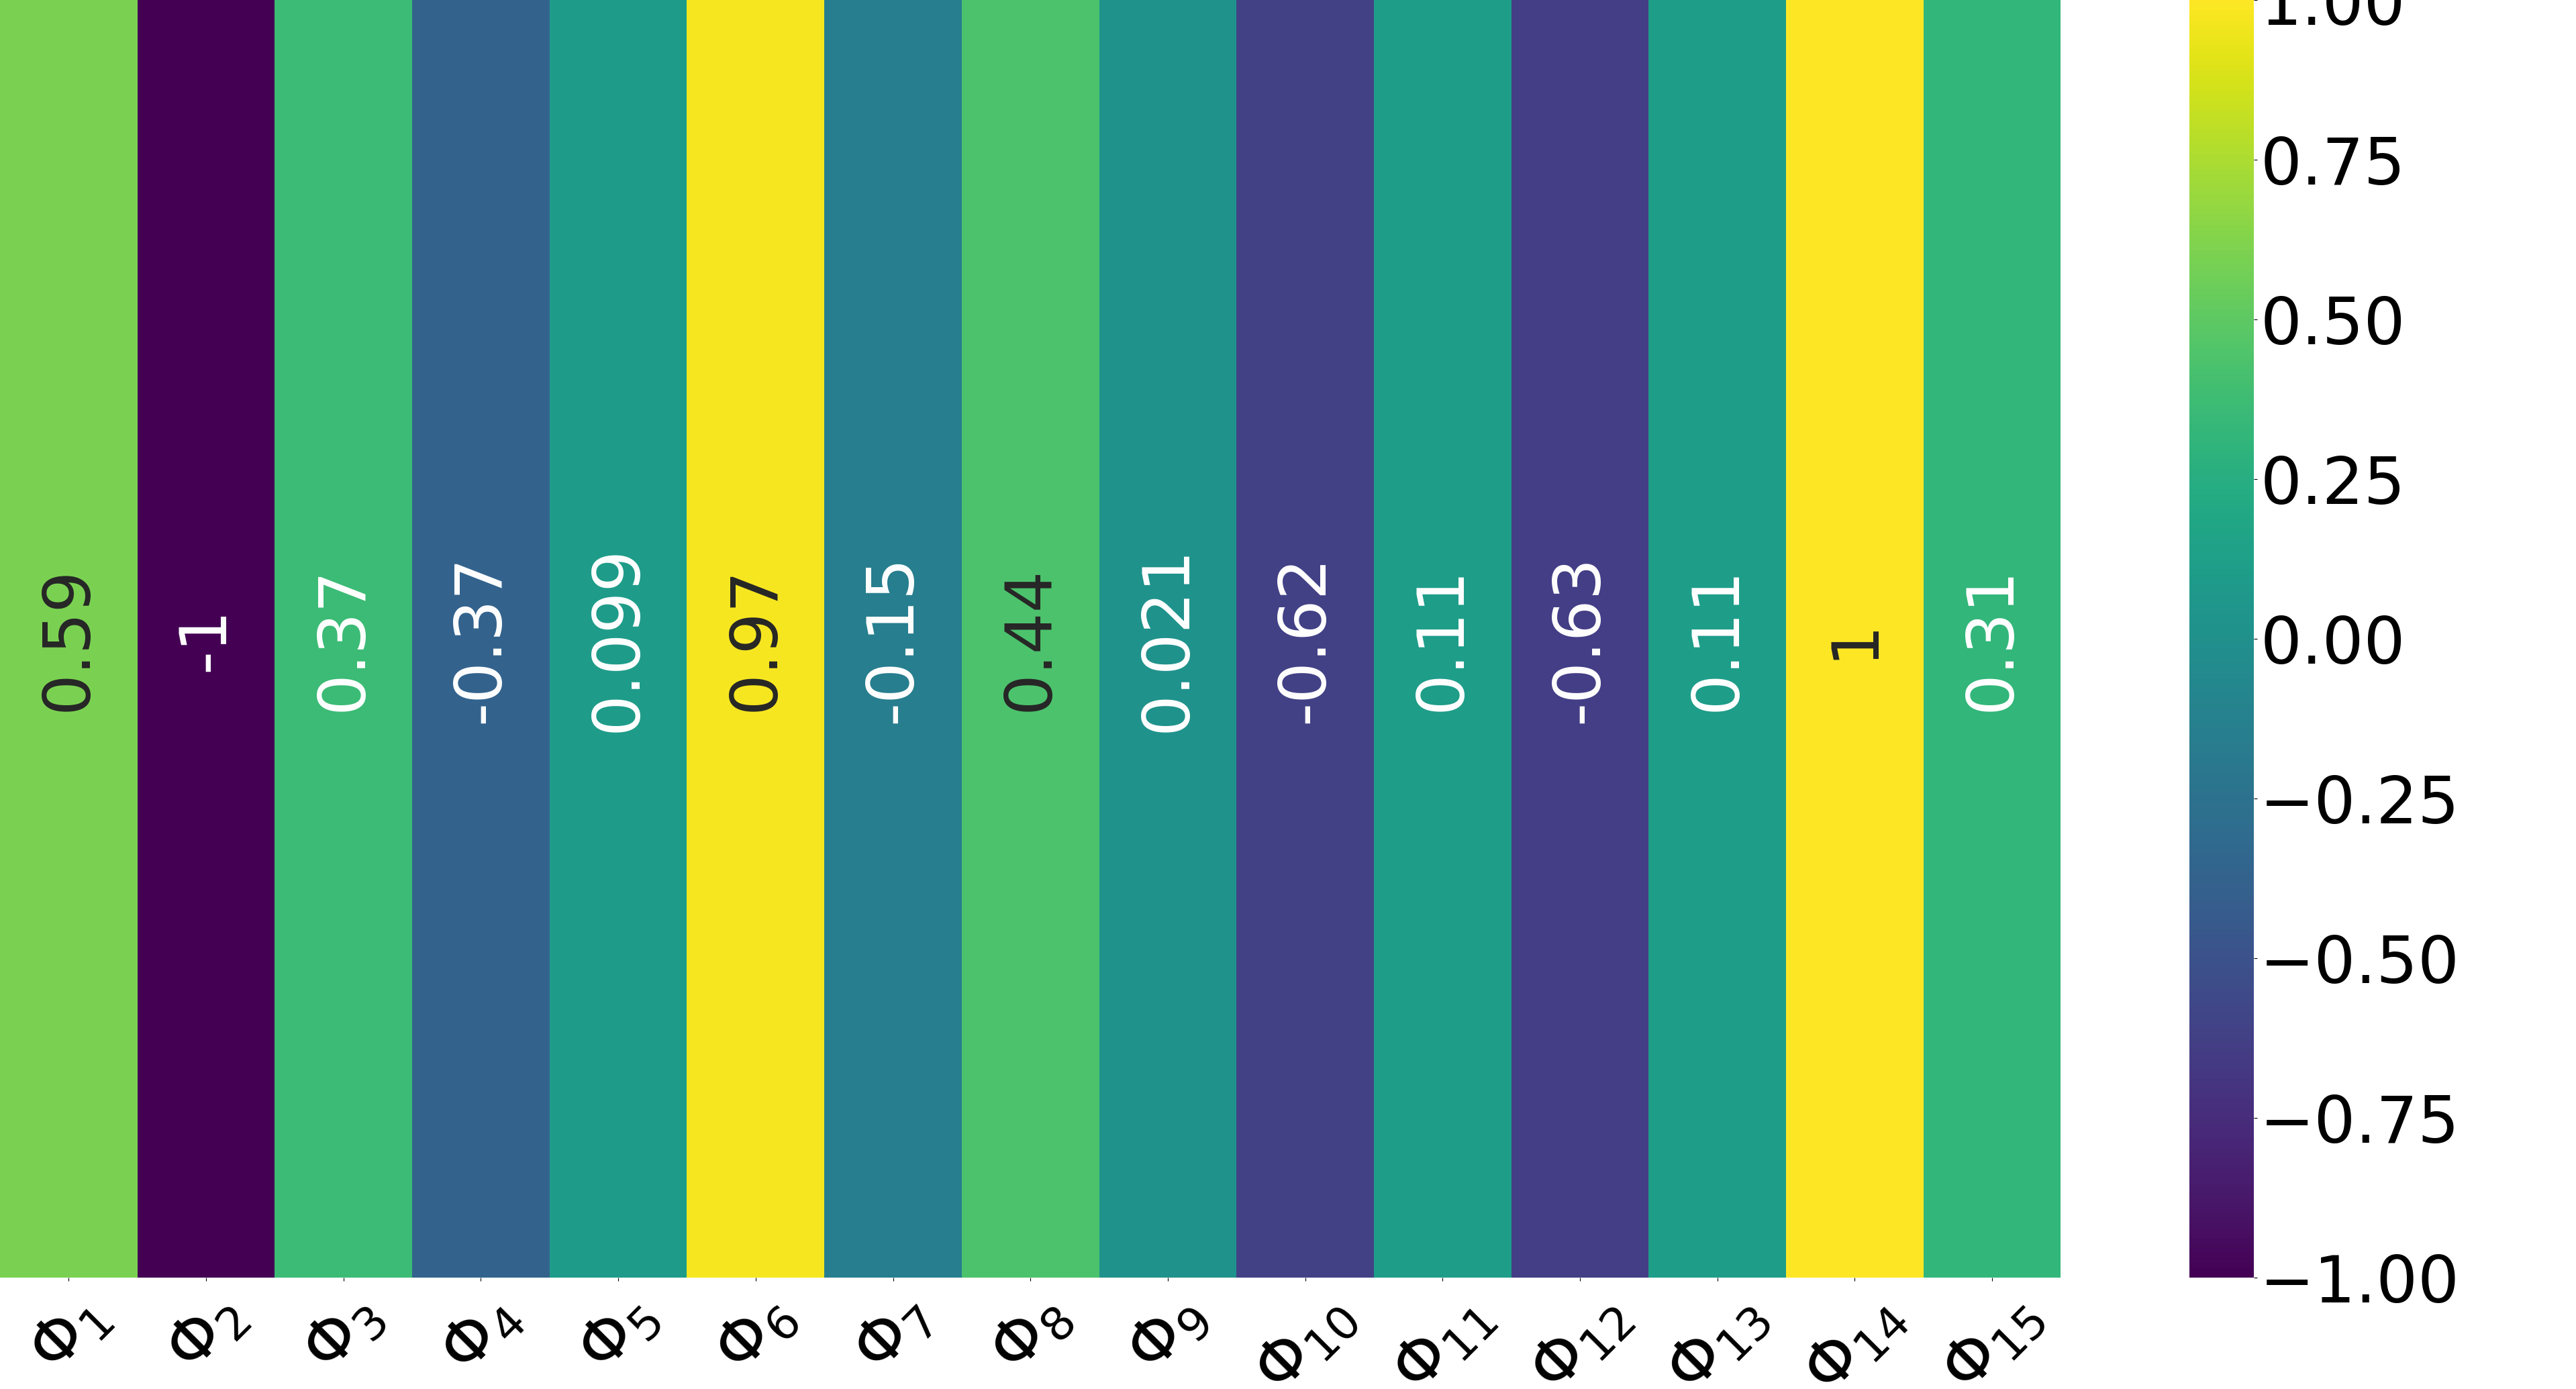
\includegraphics[width=0.7\linewidth]{img/Phi_label_corr.png}
	\caption{Correlation between the harmonics and the labels for \phin.} \label{fig:phi-lcorr}
\end{figure}

\medskip

This closes the brief exposition about the preprocessing steps for the various attributes, now we will
tackle the model selection procedure indicating which were the best models overall and which model
we chose to solve \qrp.

\section{Results}
\label{sec:results-qrp}
Every model shown in this section has been tested using the nested Cross-Validation procedure
outlined in \Cref{sec:cv} (unless otherwise stated). In this section we will discuss the results obtained for the various models
introduced in \Cref{chp:ml}.

\subsection{Decision trees}
\label{sec:qrp-dt}
As we already alluded to in previous sections we wanted to find a highly explainable model with good
performance that could be used to solve \qrp, we deemed \dts\ the best possible starting point.

With our experiments we tried different approaches and different datasets. After a careful analysis
we found that the best \dts\ were based on \an; the best classifier, trained \an[2] and \an[12],
makes only $4$ errors total: $3$ false negatives (quench events that were predicted non-quenches)
and $1$ false positive (non-quench predicted as quench event). The performance of the model,
averaged over the outer \cv\ folds, is reported in \Cref{tbl:an-2-12-perf}, as we can see, the
numbers are already very solid; showing high averages and low standard deviations. This implies that
the performance difference between the worst and the best folds is very marginal, thus the models on
the various folds perform quite similarly.
\begin{table}[!ht]
	\caption{Average and standard deviation of the performance for the best \dt\ over the outer \cv\
		folds.}\label{tbl:an-2-12-perf}

	\bigskip
	\setlength{\tabcolsep}{6pt}
	\centering
	\begin{tabular}{ccccccc}
		\toprule
		\textbf{}    & \textbf{Acc} & \textbf{Prc} & \textbf{Rec} & \textbf{Irec} & \textbf{F1} & \textbf{RAUC} \\
		\midrule
		Mean         & 0.984        & 0.994        & 0.983        & 0.988         & 0.988
		             & 0.989                                                                                    \\
		\textsc{std} & 0.008        & 0.011        & 0.014        & 0.025         & 0.006
		             & 0.012                                                                                    \\
		\bottomrule
	\end{tabular}
\end{table}

\Cref{fig:dt-an-2-12-pt} shows the structure of the decision tree, built on \an[2] and \an[12], the
tree is extremely simple, with a depth of just $2$, using mostly \an[2] to perform the splits, and
having only one node where the impurity is not zero (the light-orange in the left section of the
image).
\begin{figure}[!ht]
	\centering
	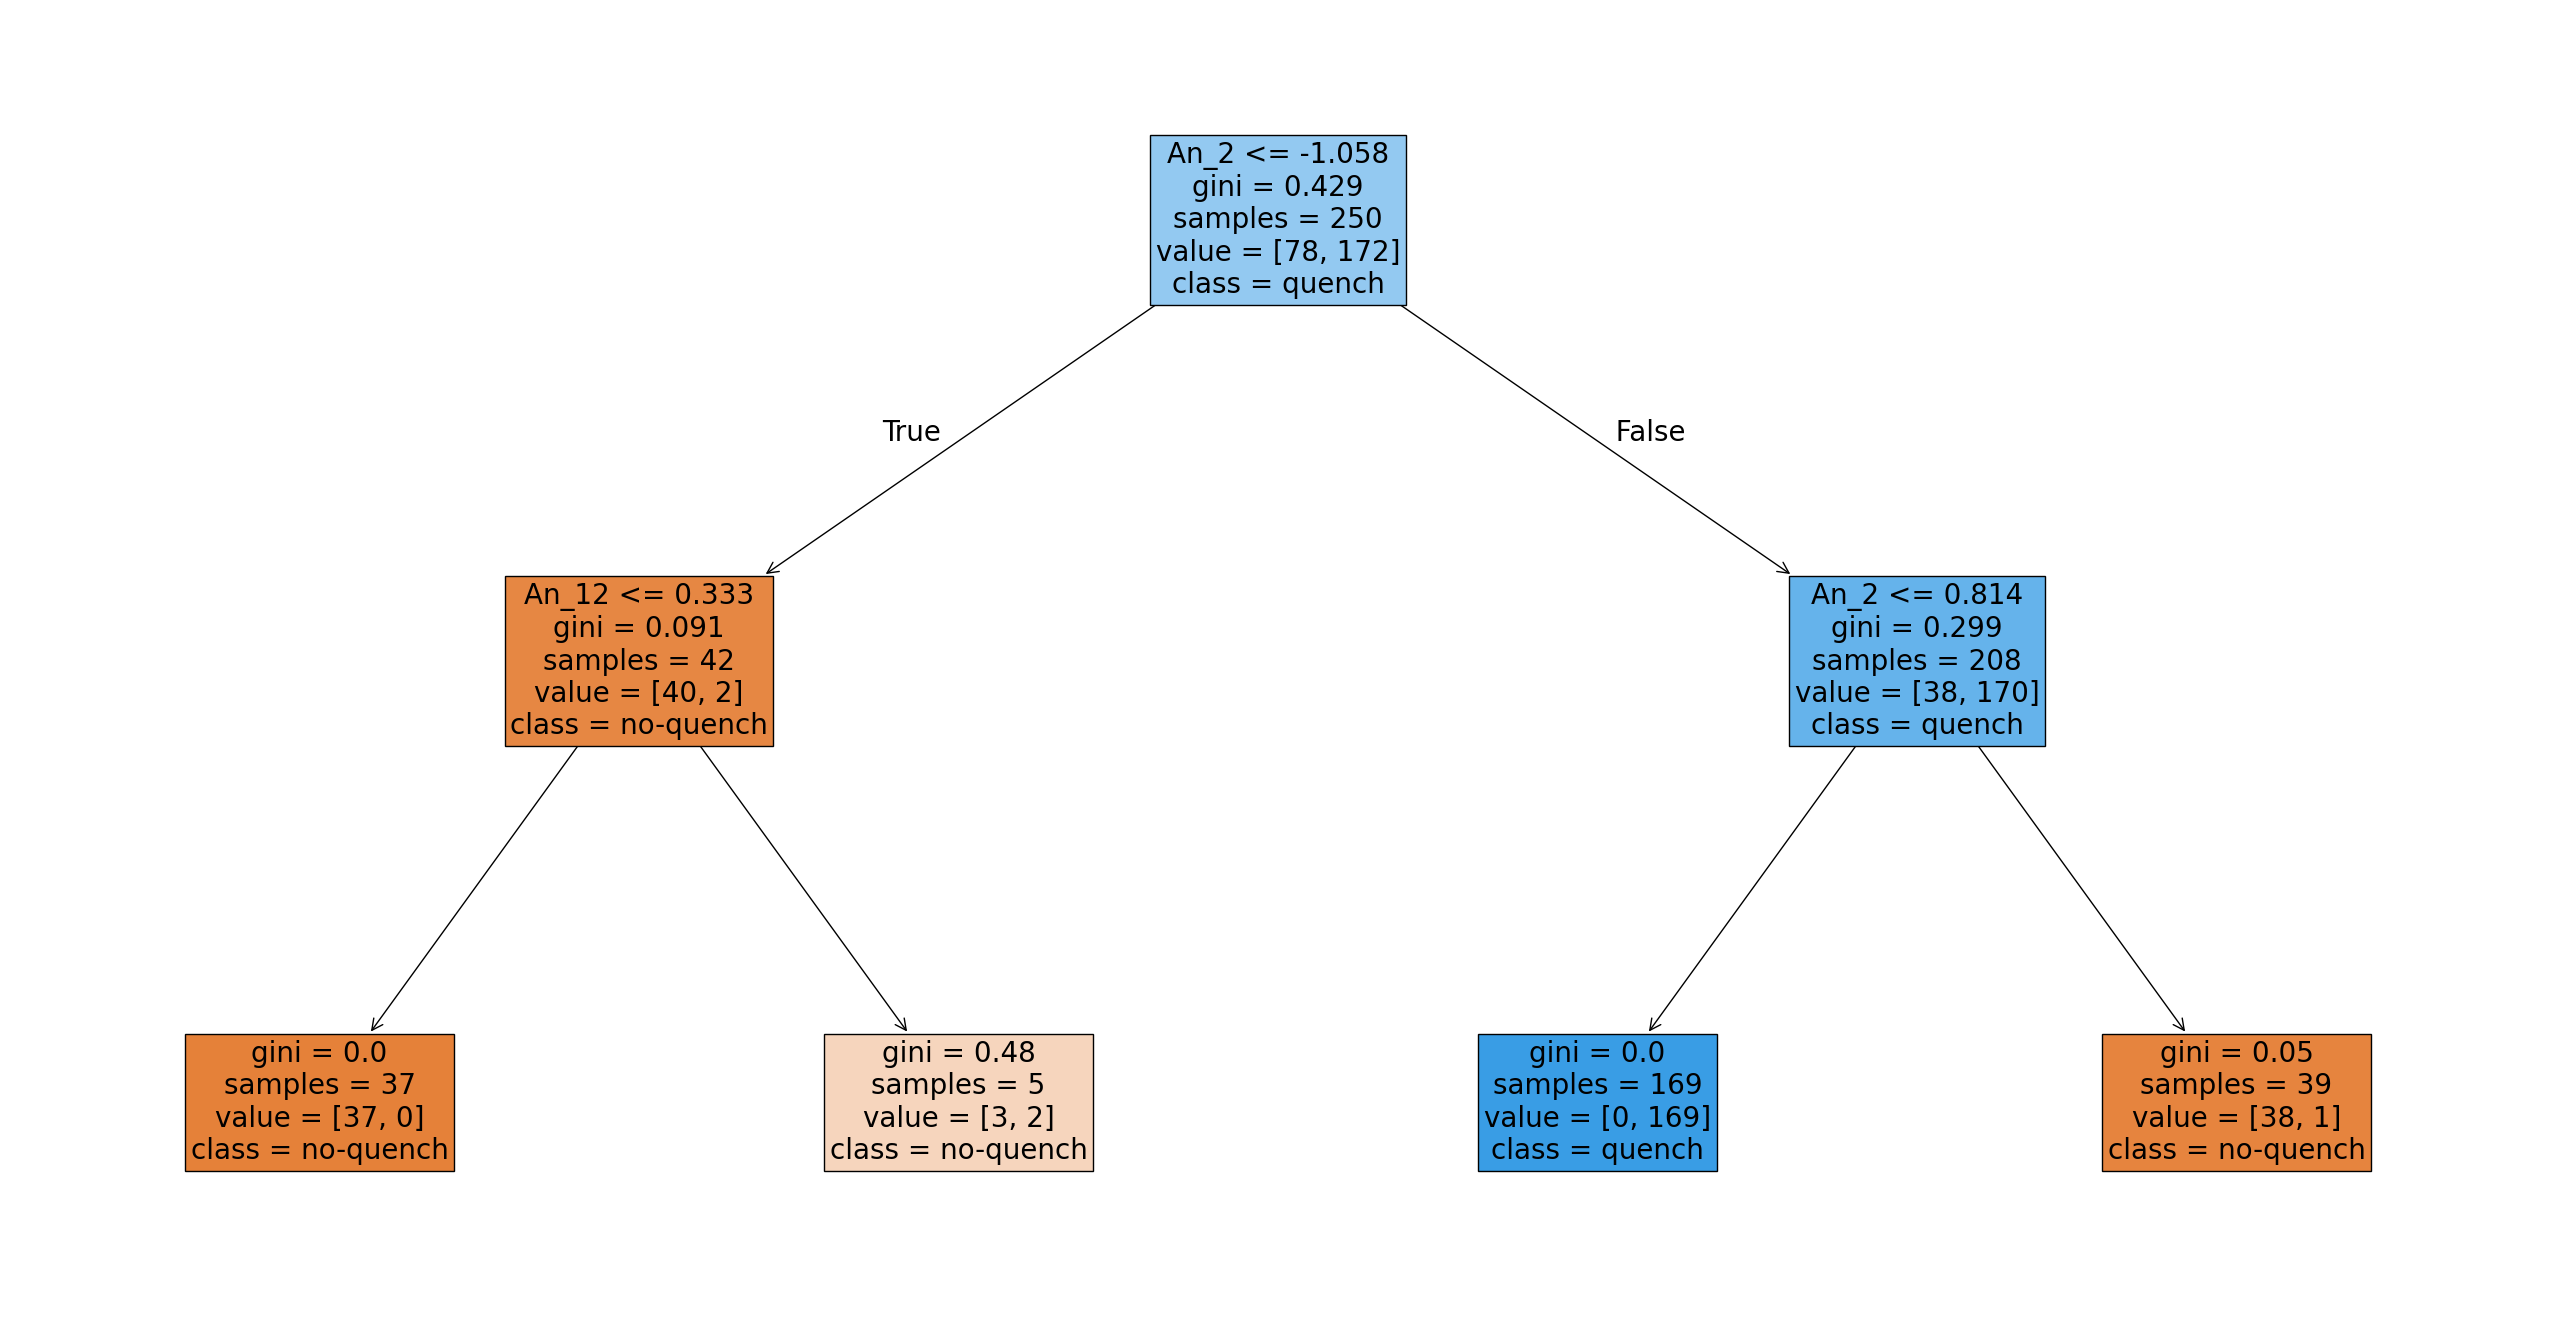
\includegraphics[width=0.7\linewidth]{img/An_2_12_pt_dt.png}
	\caption{The structure of the tree built on \an[2] and \an[12]} \label{fig:dt-an-2-12-pt}
\end{figure}

Many \dts\ were trained on different sub-views of the available attributes, but all of them fell short
of the classifier just described. In \Cref{fig:best-dts} we plotted the best \dt\ for every
attribute against each other, despite \cnmod\ having similar accuracy to the classifier just
described, it cannot recognize non-quench events as effectively (the Irec score is lower).
\begin{figure}[!ht]
	\centering
	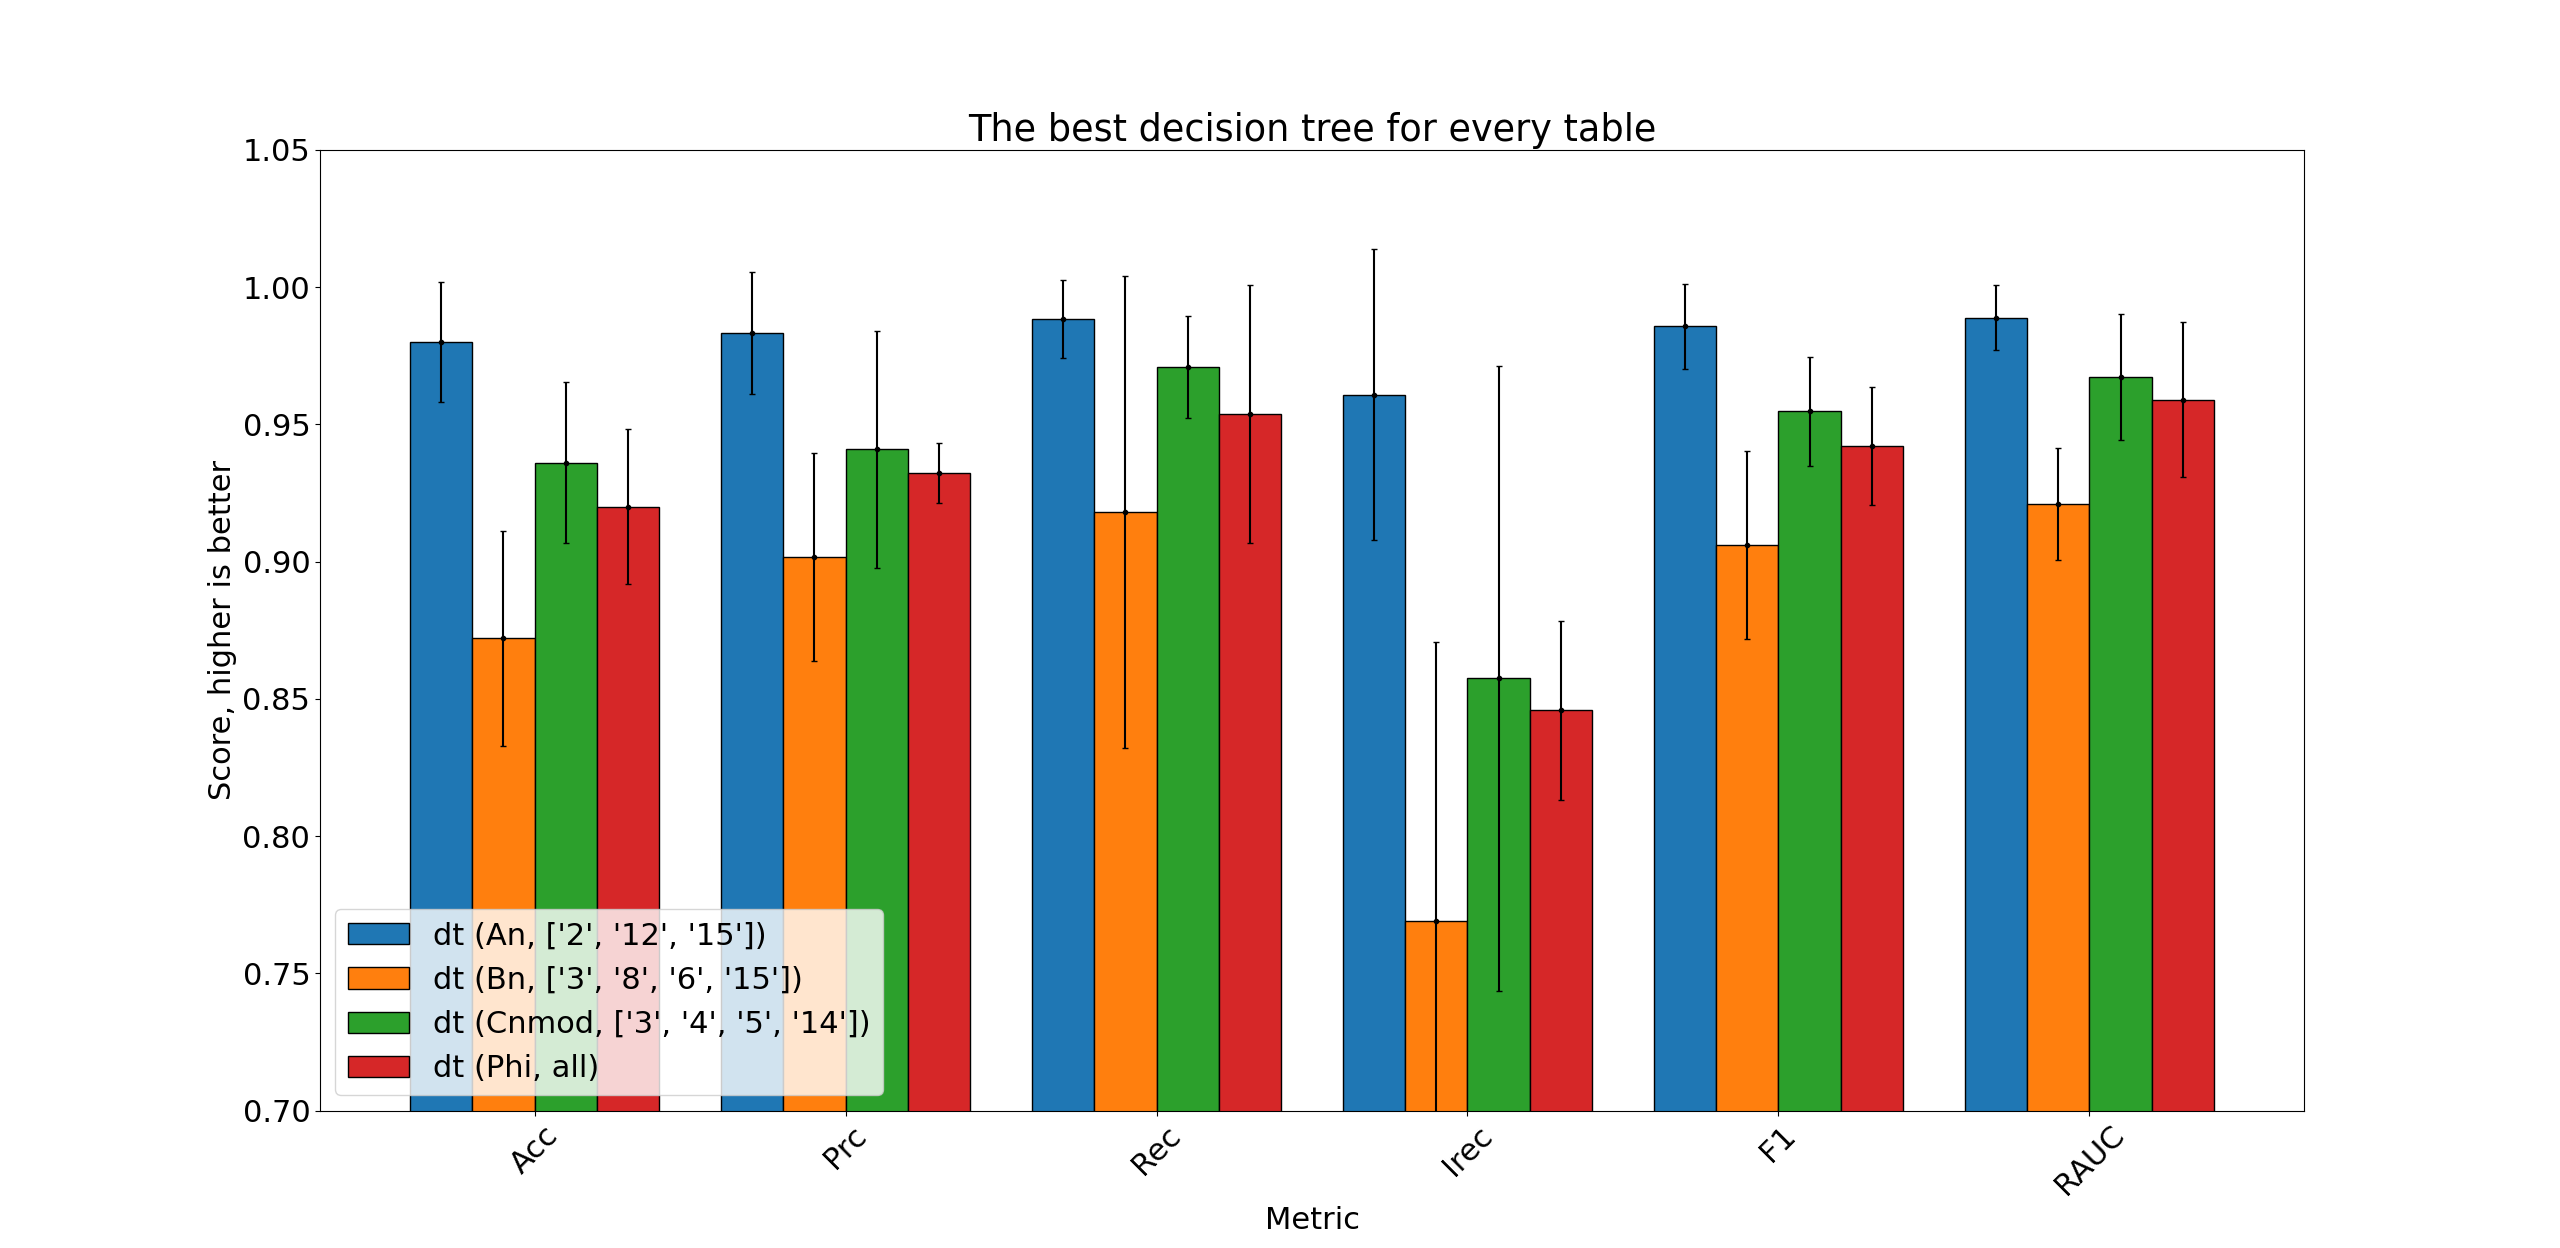
\includegraphics[width=0.7\linewidth]{img/best_dts.png}
	\caption{Performance comparison of the best decision tree for each attribute. The
		performance plotted here are average and standard deviation of the metrics calculated on the
		outer loop of the \ncv.} \label{fig:best-dts}
\end{figure}

Finally, if we use our blind-test set \db, we can see that the best model, trained on a sub-view of
\an\ containing only \an[2], and \an[12] misclassifies only two samples, one false positive and one
false negative. The final performance metrics are listed in \Cref{tbl:blind-test-bdt}
\begin{table}[!ht]
	\setlength{\tabcolsep}{6pt}
	\centering
	\begin{tabular}{cccccc}
		\toprule
		\textbf{Acc} & \textbf{Prc} & \textbf{Rec} & \textbf{F1} & \textbf{Irec} & \textbf{RAUC} \\
		\midrule
		0.931        & 0.950        & 0.950        & 0.950       & 0.889         & 0.919         \\
		\bottomrule
	\end{tabular}
	\caption{Score computed on the blind-test done on the best decision tree, the metrics have
		been computed on the $29$ samples contained in the dataset.}\label{tbl:blind-test-bdt}
\end{table}

\subsection{Random Forests}
\label{sec:qrp-rf}
As we said in \Cref{chp:ml}, random forests (\rfs) use an ensemble of trees trained by bootstrap
sampling and perform splits on a random subset of features. As long as the trees are not too
complex, and the ensemble is not too big, \rfs\ are still quite easy to interpret. We expect
performance to be at least as good, if not better, than the worst tree in the ensemble (cfr.
\cref{chp:ml}). Since a single \rf\ contains more \dts\, they can extrapolate more information from
complicated datasets containing different sub-views (e.g., a dataset containing a sub-view for each
of \an, \bn and \cnmod).

In most of our tests we considered \rfs\ trained on datasets built from one or more attributes, each
taken in its entirety. We also did some tests on forests built on datasets containing sub-views for
one or more attributes. While the second approach was more suitable for raw performance, the first
one gave us insights, through the \emph{feature importance} metric, of which were the more important
harmonics within the dataset.

Feature importance is a measure that we can use to understand which features are more prominent in
the \rf\ structure, this can give us insights on how to better design the sub-views used for model
training. We analyzed the feature importance of \rfs\ built on single attributes (e.g., a \rf\
trained only on \an) and then of a \rf\ constructed on the whole dataset, we concluded that:
\begin{itemize}
	\item The forest built on \an, performs most of the splits ($\approx 80\%$) using \an[2].
	\item The forest built on \bn, performs most of the splits using a mix of different
	      harmonics: \bn[6], \bn[9], \bn[3], \bn[14], \bn[7] and \bn[5] are the ones used the most.
	\item The forest built on \cnmod, uses \cnmod[2] to perform over $50\%$ of the splits, the
	      rest are handled mainly via \cnmod[5], \cnmod[9] and \cnmod[13].
	\item The forest built on \phin, uses many different harmonics to perform the splits (mainly
	      \phin[10], \phin[12] and \phin[6]).
	\item If we train a forest on the whole dataset, we can see that $\approx90\%$ of the splits
	      were computed by using \cnmod[2], \cnmod[3], \an[12], \an[2] and \an[14]. This is very
	      interesting because it corroborates the hypothesis that \cnmod\ and \an\ are
	      important attributes for \qrp.
\end{itemize}

In \Cref{fig:best-rfs} we plotted the metrics for the $4$ best performing random forests,
independently of the dataset they were trained on, the best model achieved accuracy of
$\approx 98.8\%$, while the others average around $98\%$.
\begin{figure}[!ht]
	\centering
	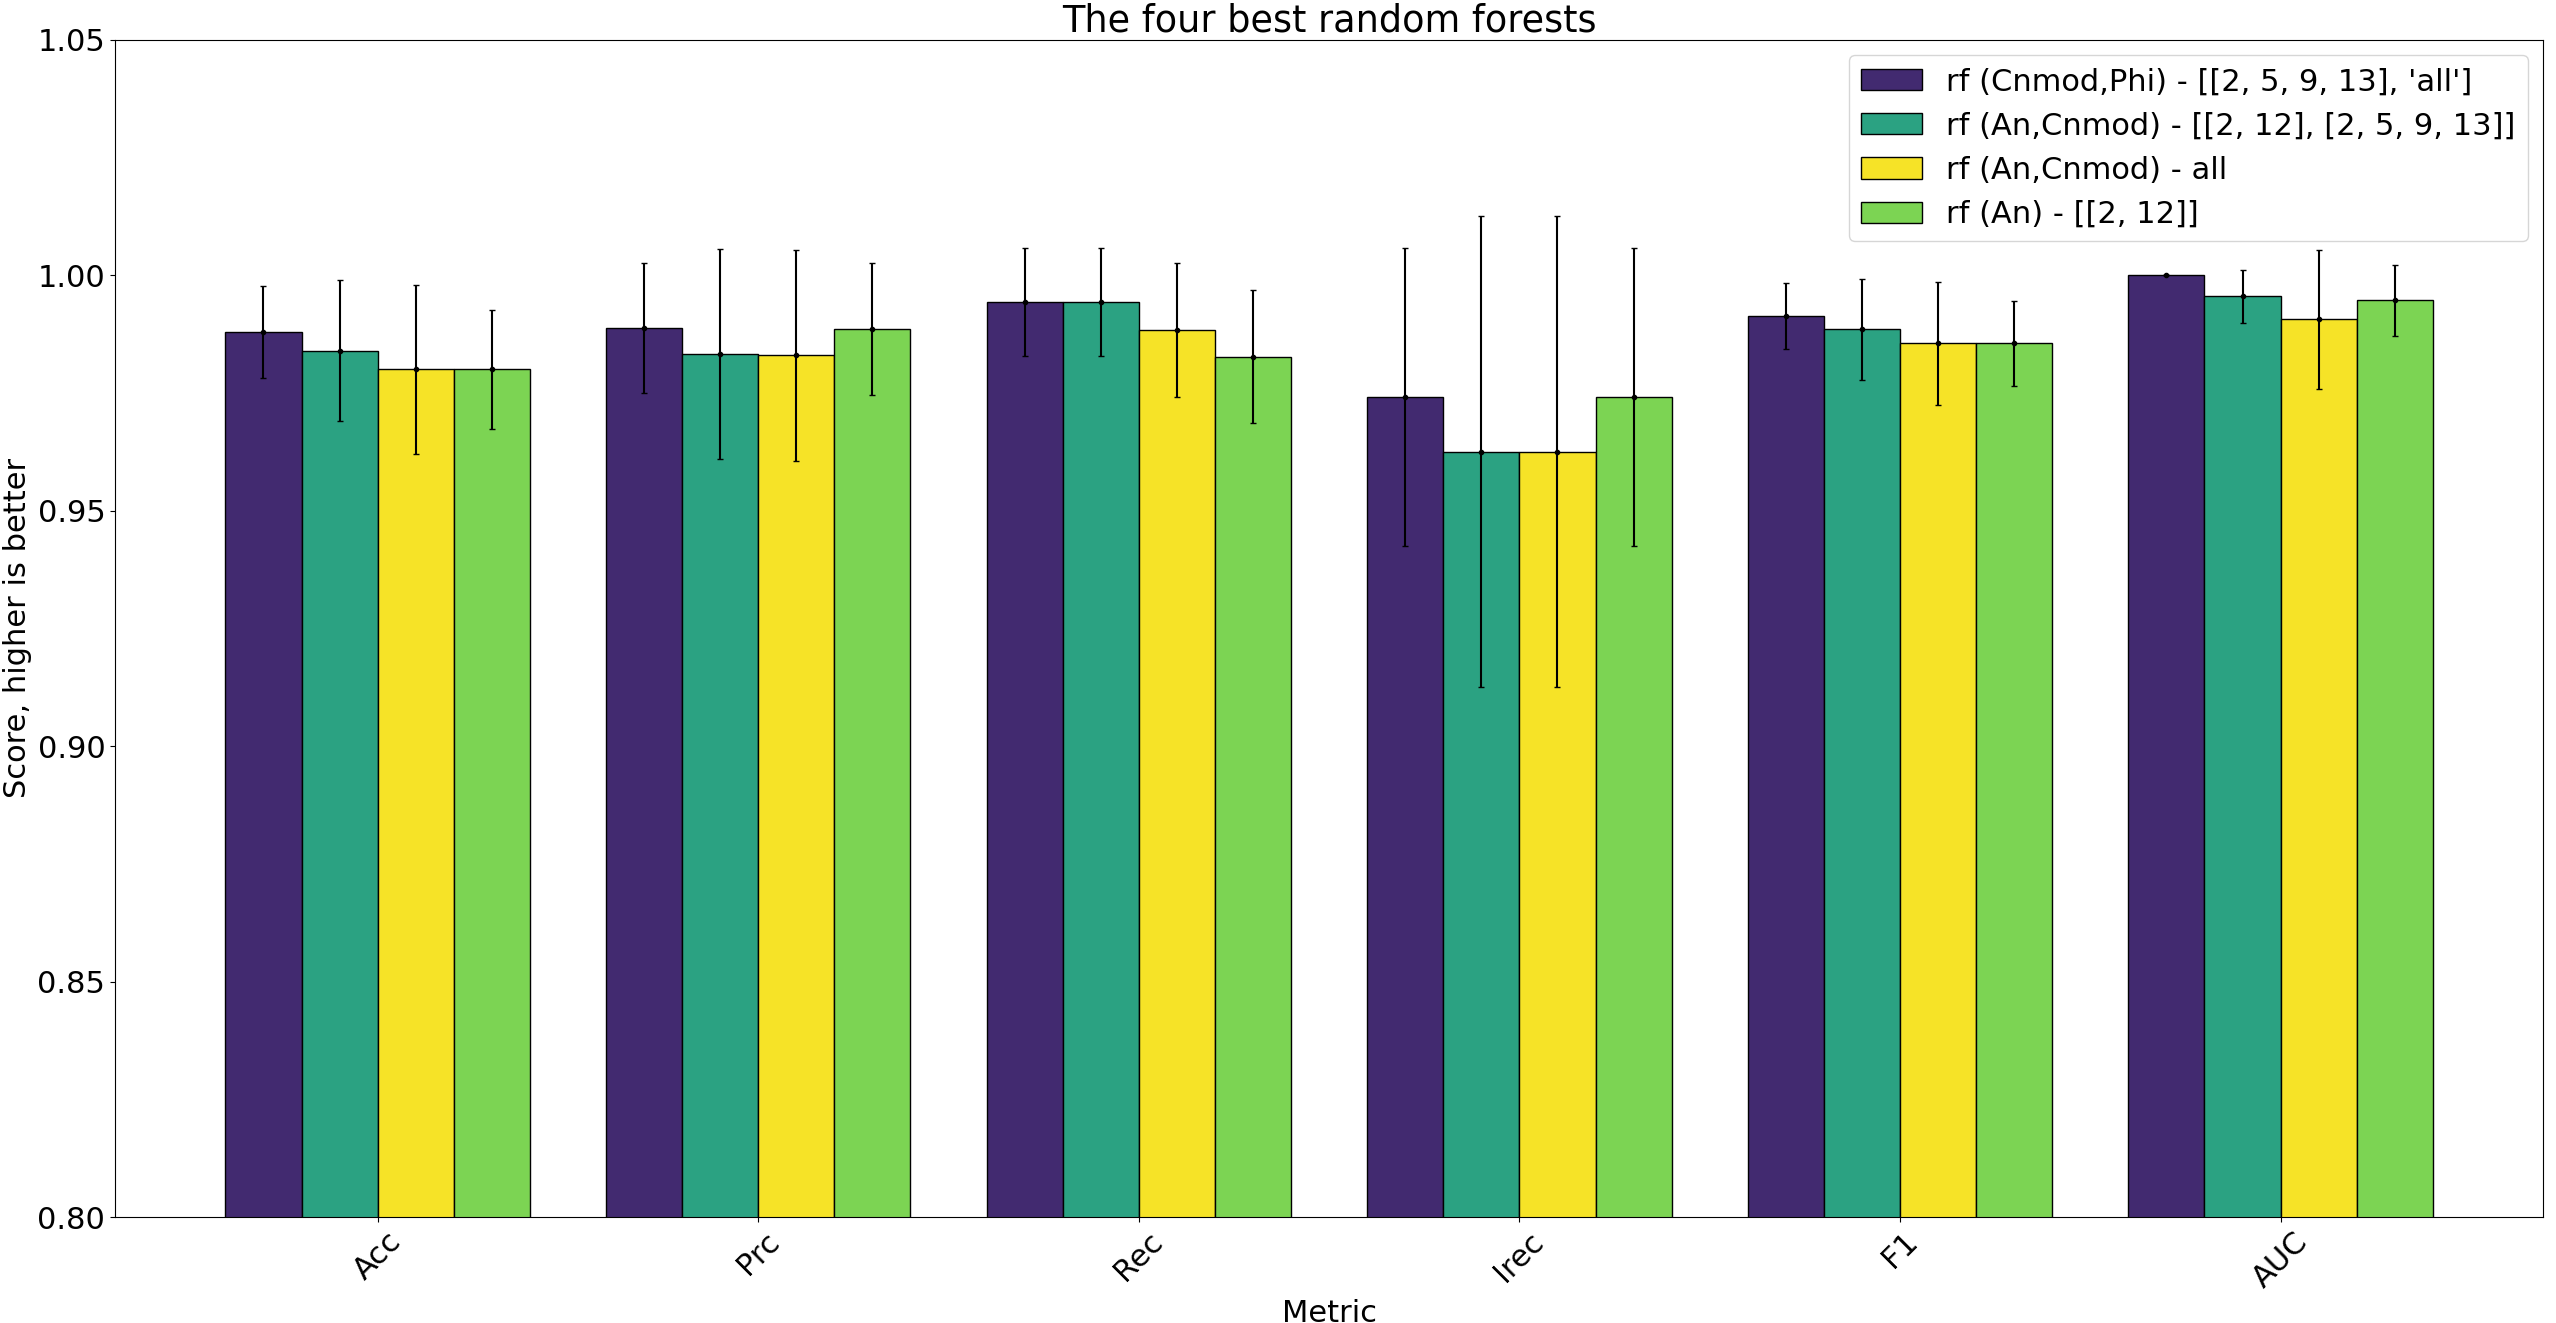
\includegraphics[width=0.7\linewidth]{img/best_rfs.png}
	\caption{Performance for the $4$ highest performing forests, independently of which
		dataset they were trained on, the plotted measurements are the average for each metric and
		the standard deviation, each computed on the outer loop of \ncv.} \label{fig:best-rfs}
\end{figure}

In \Cref{tbl:rf-cnmod-phi-perf} we reported the performance for the best \rf. While good, we could probably achieve better
results, since the models we tested were trained on datasets containing different sub-views\footnote{
	Which is very different from grouping trees trained on different sub-views.
}; regardless of the correlation among harmonics belonging to different attributes, which is
definitely a very important factor to keep in mind. We decided not to explore this solution more
since, as we will see briefly, \rfs\ can be more complicated to interpret than a model we devised,
which will be introduced in \Cref{sec:qrp-ta}.
\begin{table}[!ht]
	\caption{Average and standard deviation for each metric computed on the best \rf\ in the outer \cv\ folds.}\label{tbl:rf-cnmod-phi-perf}

	\bigskip
	\setlength{\tabcolsep}{6pt}
	\centering
	\begin{tabular}{ccccccc}
		\toprule
		\textbf{}    & \textbf{Acc} & \textbf{Prc} & \textbf{Rec} & \textbf{Irec} & \textbf{F1} & \textbf{RAUC} \\
		\midrule
		Mean         & 0.988        & 0.989        & 0.994        & 0.974         & 0.991
		             & 1.0                                                                                      \\
		\textsc{std} & 0.010        & 0.013        & 0.011        & 0.032         & 0.007
		             & 0.0                                                                                      \\
		\bottomrule
	\end{tabular}
\end{table}
%{'accuracy-mean': np.float64(0.9879999999999999), 'accuracy-std': np.float64(0.009797958971132722), 'precision-mean': np.float64(0.9887301587301588), 'precision-std': np.float64(0.01380496184454534), 'recall-mean': np.float64(0.9942857142857143), 'recall-std': np.float64(0.011428571428571432), 'inv-recall-mean': np.float64(0.9741666666666667), 'inv-recall-std': np.float64(0.03166666666666666), 'f1-mean': np.float64(0.991385997142274), 'f1-std': np.float64(0.0070348834762717265), 'roc_auc-mean': np.float64(1.0), 'roc_auc-std': np.float64(0.0)}

The best \rf\ contains $5$ trees, each has a maximum depth of $4$ and the number of
internal nodes and leaves is always quite limited (on average the trees inside the forest contain
$4$ internal nodes). The most important harmonics are \cnmod[2], \cnmod[5], \phin[6]\ and \phin[10].
If we test the model on the blind-test set, \db, we see that the classifier only makes one classification error among the $29$ samples, specifically a false positive.
\begin{table}[!ht]
	\caption{Performance metrics for the best \rf\ computed on the $29$ samples in the
		blind-test set.}\label{tab:qrp-rf-test}

	\bigskip
	\setlength{\tabcolsep}{6pt}
	\centering
	\begin{tabular}{cccccc}
		\toprule
		\textbf{Acc} & \textbf{Prc} & \textbf{Rec} & \textbf{F1} & \textbf{Irec} & \textbf{RAUC} \\
		\midrule
		0.965        & 0.952        & 1            & 0.976       & 0.889         & 0.944         \\
		\bottomrule
	\end{tabular}
\end{table}

\subsection{SVC}
\label{sec:qrp-svc}
A binary Support Vector Classifier (\svc), is a classifier using the \svm\ architecture (cfr.
\Cref{sec:svm}). \svcs consider each sample as a vector in Euclidean space, and find a decision
surface separating the vectors corresponding to two classes. This is achieved by maximizing the
\emph{margin} we introduced in \Cref{sec:svm}, intended as the minimal distance between the decision
surface and the data images through a nonlinear mapping.

This model is meant to have very high performance at the expense of explainability, that is why we chose it as our benchmarking model.

To close the chapter dedicated to \qrp\ we will discuss Tree Aggregators (\tas).

\subsection{Tree Aggregators}
\label{sec:qrp-ta}
While the best \rf\ described in \Cref{sec:qrp-rf} has a relatively simple structure, we can still do better.

Since many of the \dts\ generated in previous phases of testing have all been serialized, and we
know how well they perform based on the performance readings obtained in the outer loop of \ncv; we
can create an ensemble of the best tree for every attribute, and then aggregate the performance by majority voting.

To test the performance of such models, which we called Tree Aggregators (\tas) to differenciate them from
\rfs, we:
\begin{itemize}
	\item aggregated the best decision tree for every attribute,
	\item retrained the single classifiers on \dr\ using a $5$-fold \cv,
	\item aggregated all the predictions via majority voting.
\end{itemize}
Since we didn't define a procedure break ties, \tas\ were tested on triplets of attributes (e.g., \an, \bn, \cnmod).

A different testing technique had to be used on \tas, since \dts\ were serialized after a retrain on
\dr\ (the $250$ samples at our disposal). This choice forced us to repeat a training procedure
whenever we wanted to test the performance of models in different configurations (like testing the
performance of \tas\ which are \dt\ ensembles built 'by hand'). Since the only unused data available
to us were the $29$ samples stored in \db, meant only for a final performance estimate.

We constructed \tas\ by aggregating three sub-views of the original dataset, and we benchmarked it
against \rfs\ trained on the best performing sub-view for each triplet and \svcs trained on
datasets simply merging the attributes in the triplet. As we can see in \Cref{fig:triplets-performance}, \tas\ usually perform
closer to \svcs\ than \rfs, with the only exception of the ROC-AUC score. Performance for the best \ta\ among the $4$ benchmarked in \Cref{fig:triplets-performance} are indicated in \Cref{tbl:an-bn-cnmod-ta-perf}.
\begin{figure}[!h]
	\centering
	\begin{subfigure}{0.49\linewidth}
		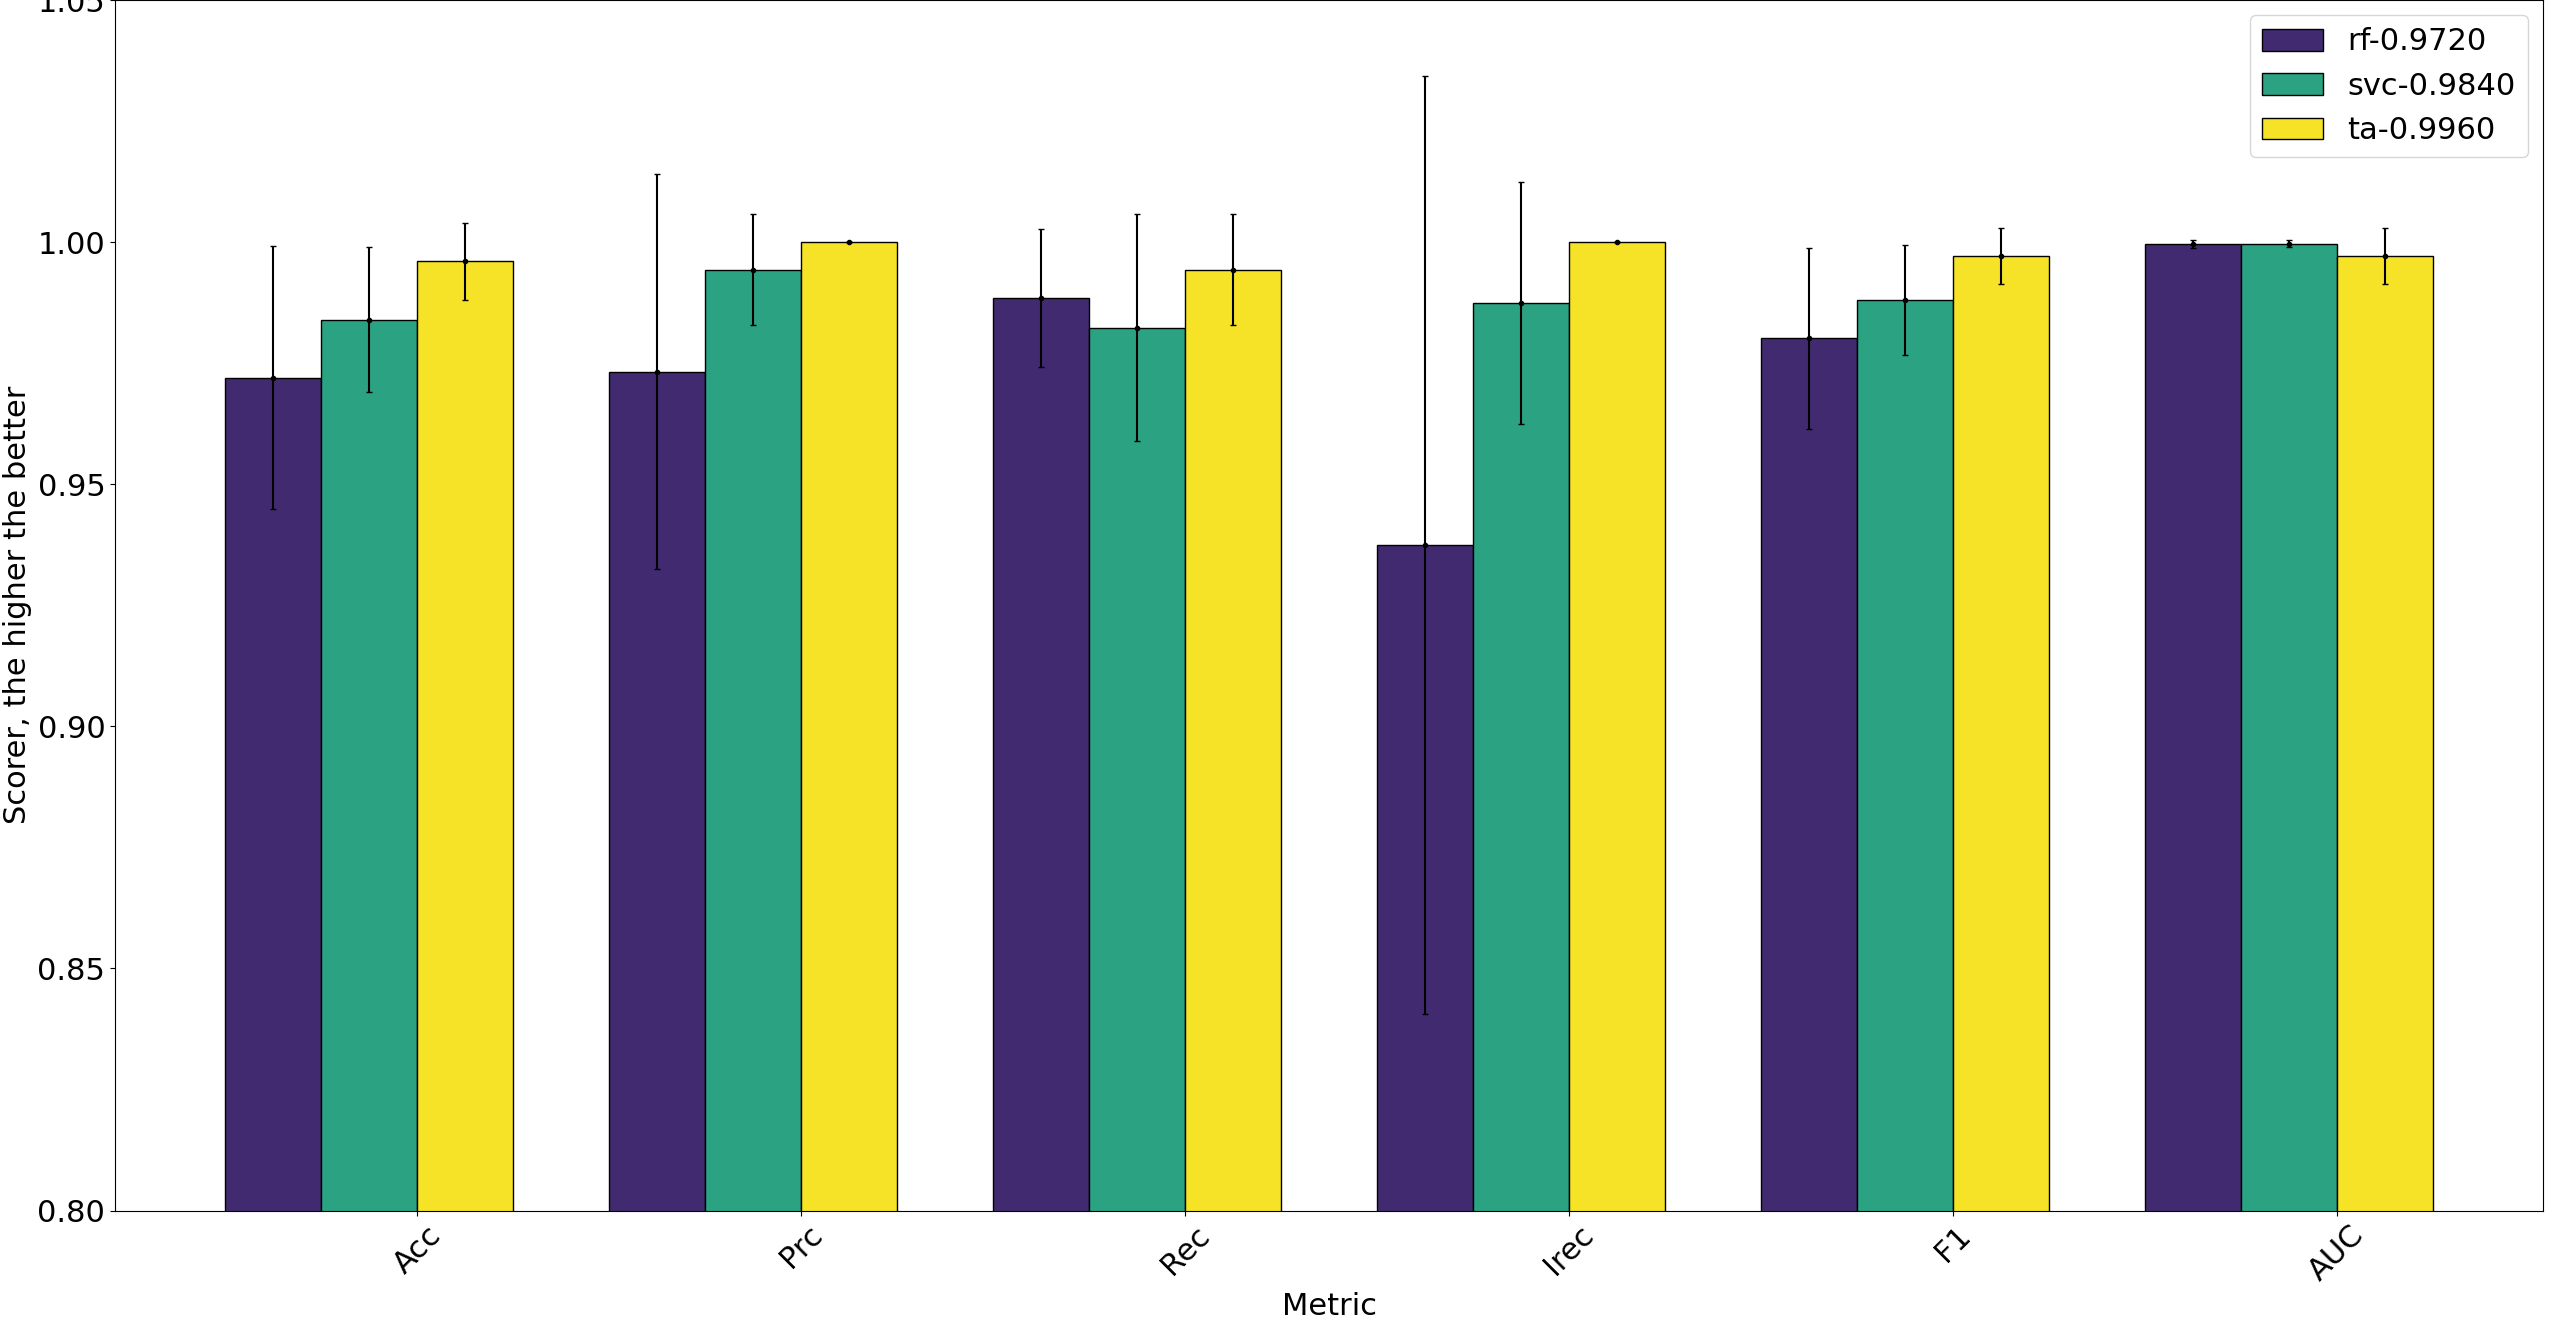
\includegraphics[width=\linewidth]{img/An_Bn_Cnmod_ta.png}
		\subcaption{\an, \bn, \cnmod}
	\end{subfigure}
	\begin{subfigure}{0.49\linewidth}
		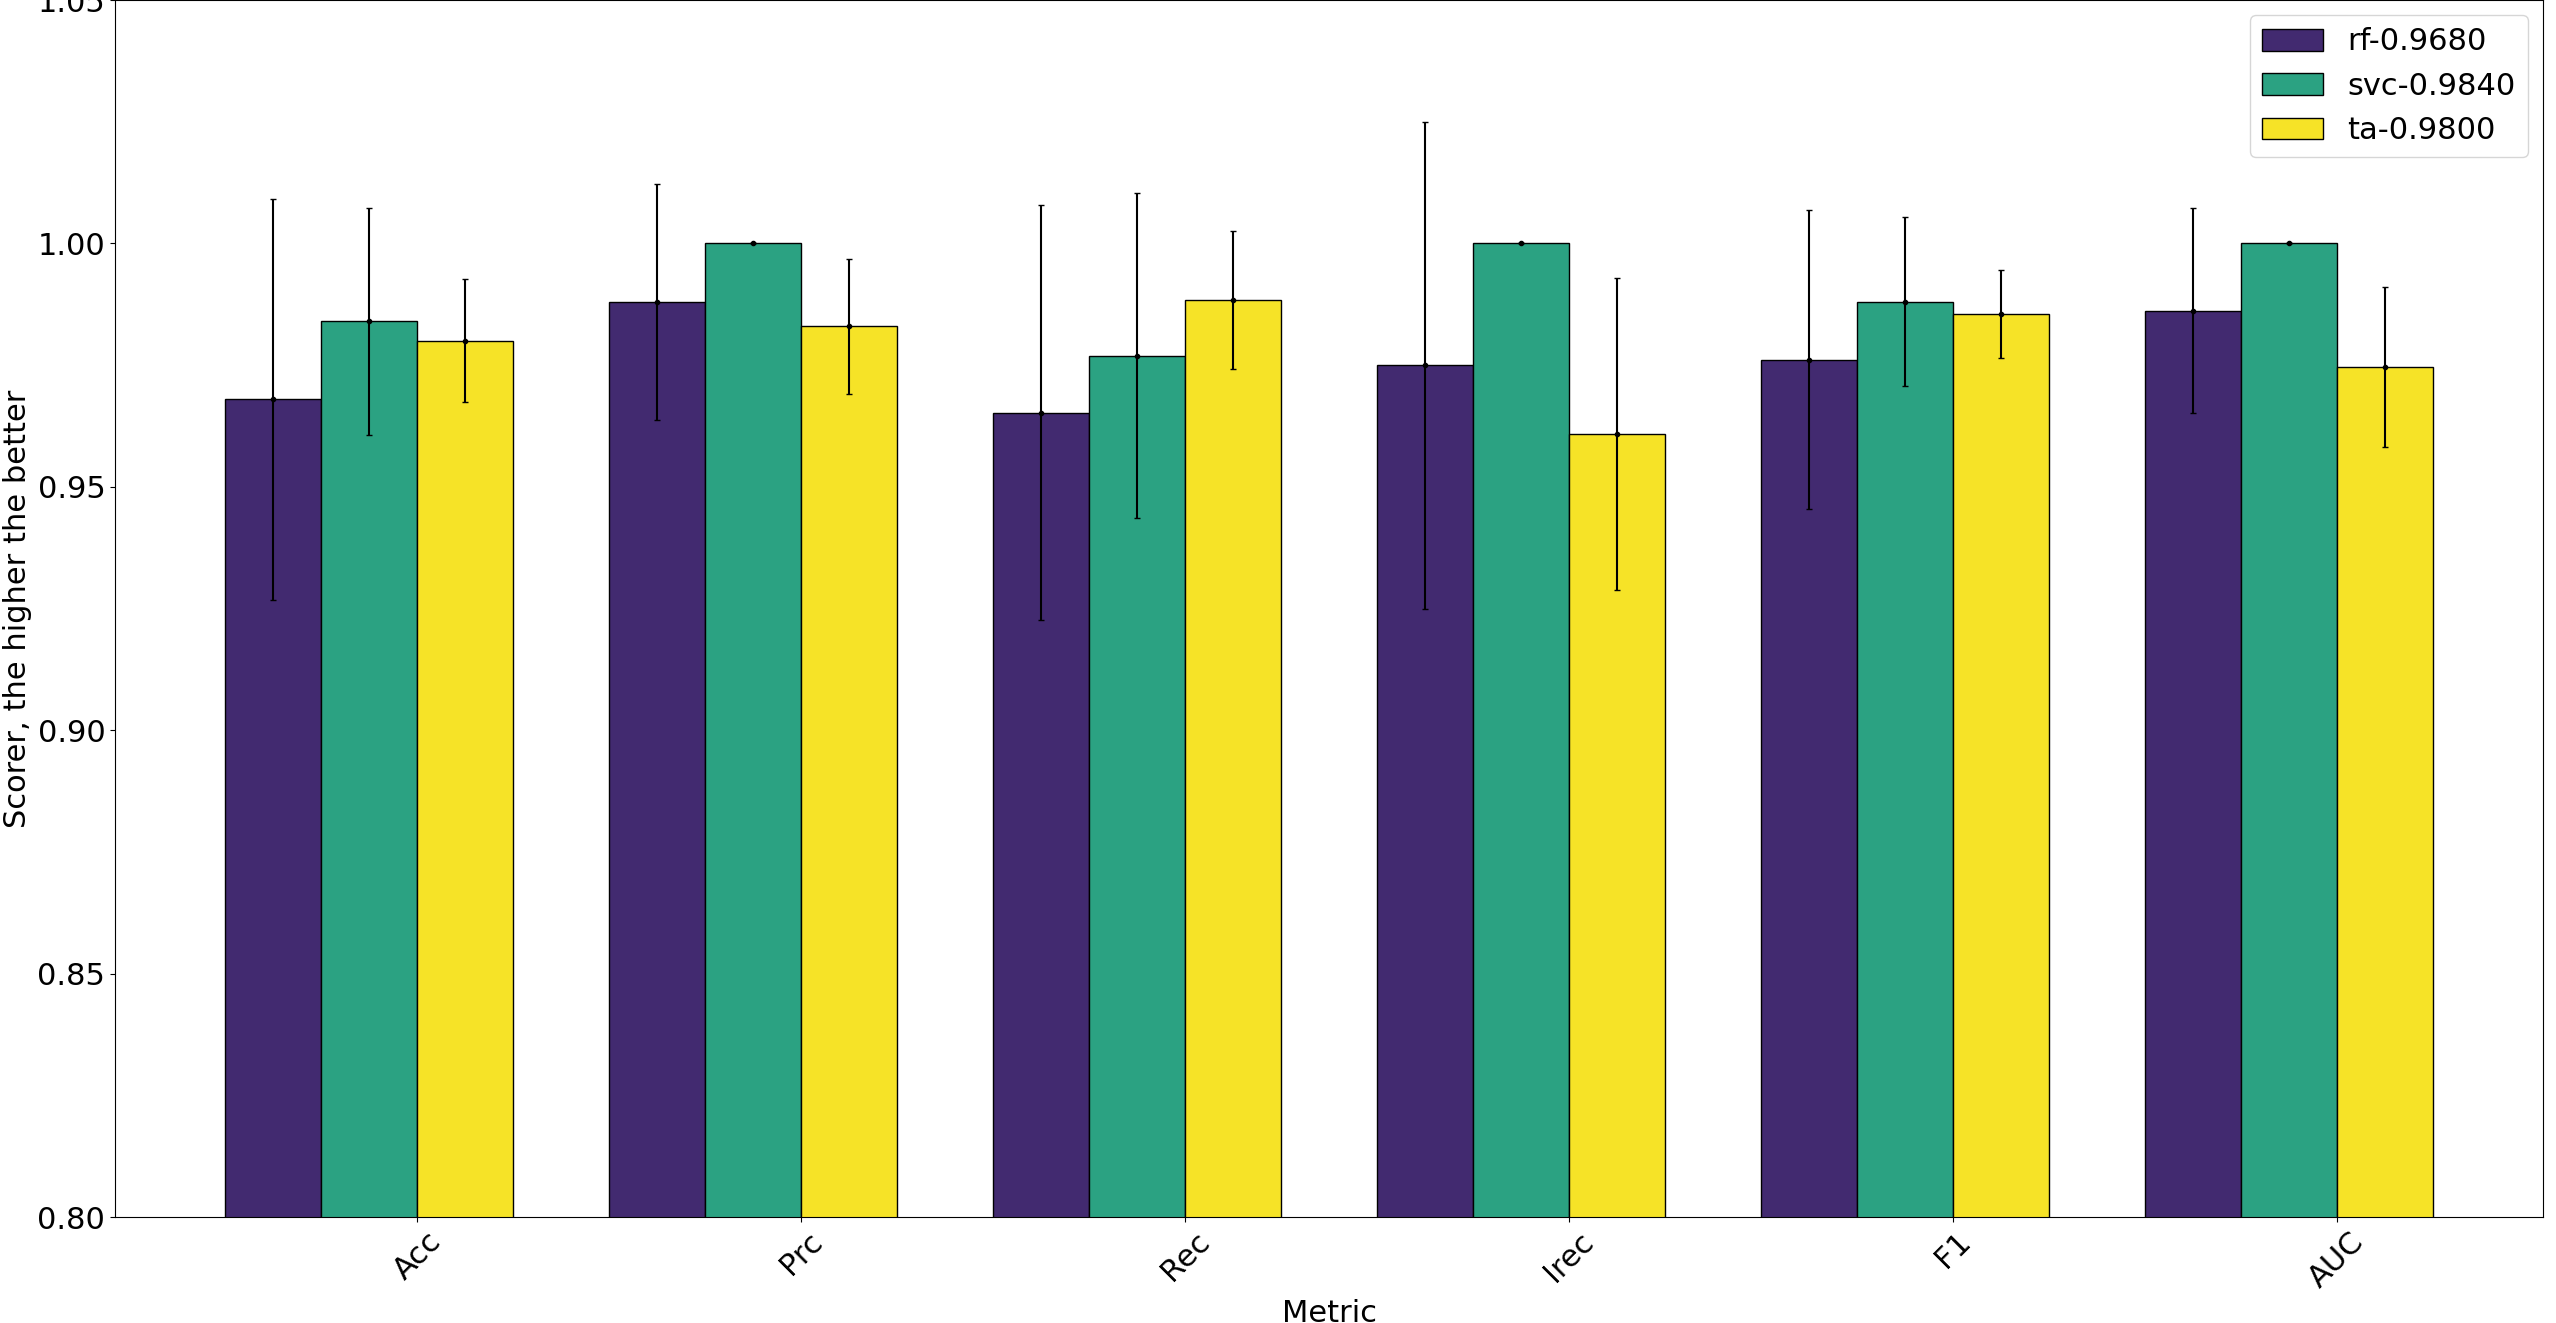
\includegraphics[width=\linewidth]{img/An_Bn_Phi_ta.png}
		\subcaption{\an, \bn, \phin}
	\end{subfigure}
	\begin{subfigure}{0.49\linewidth}
		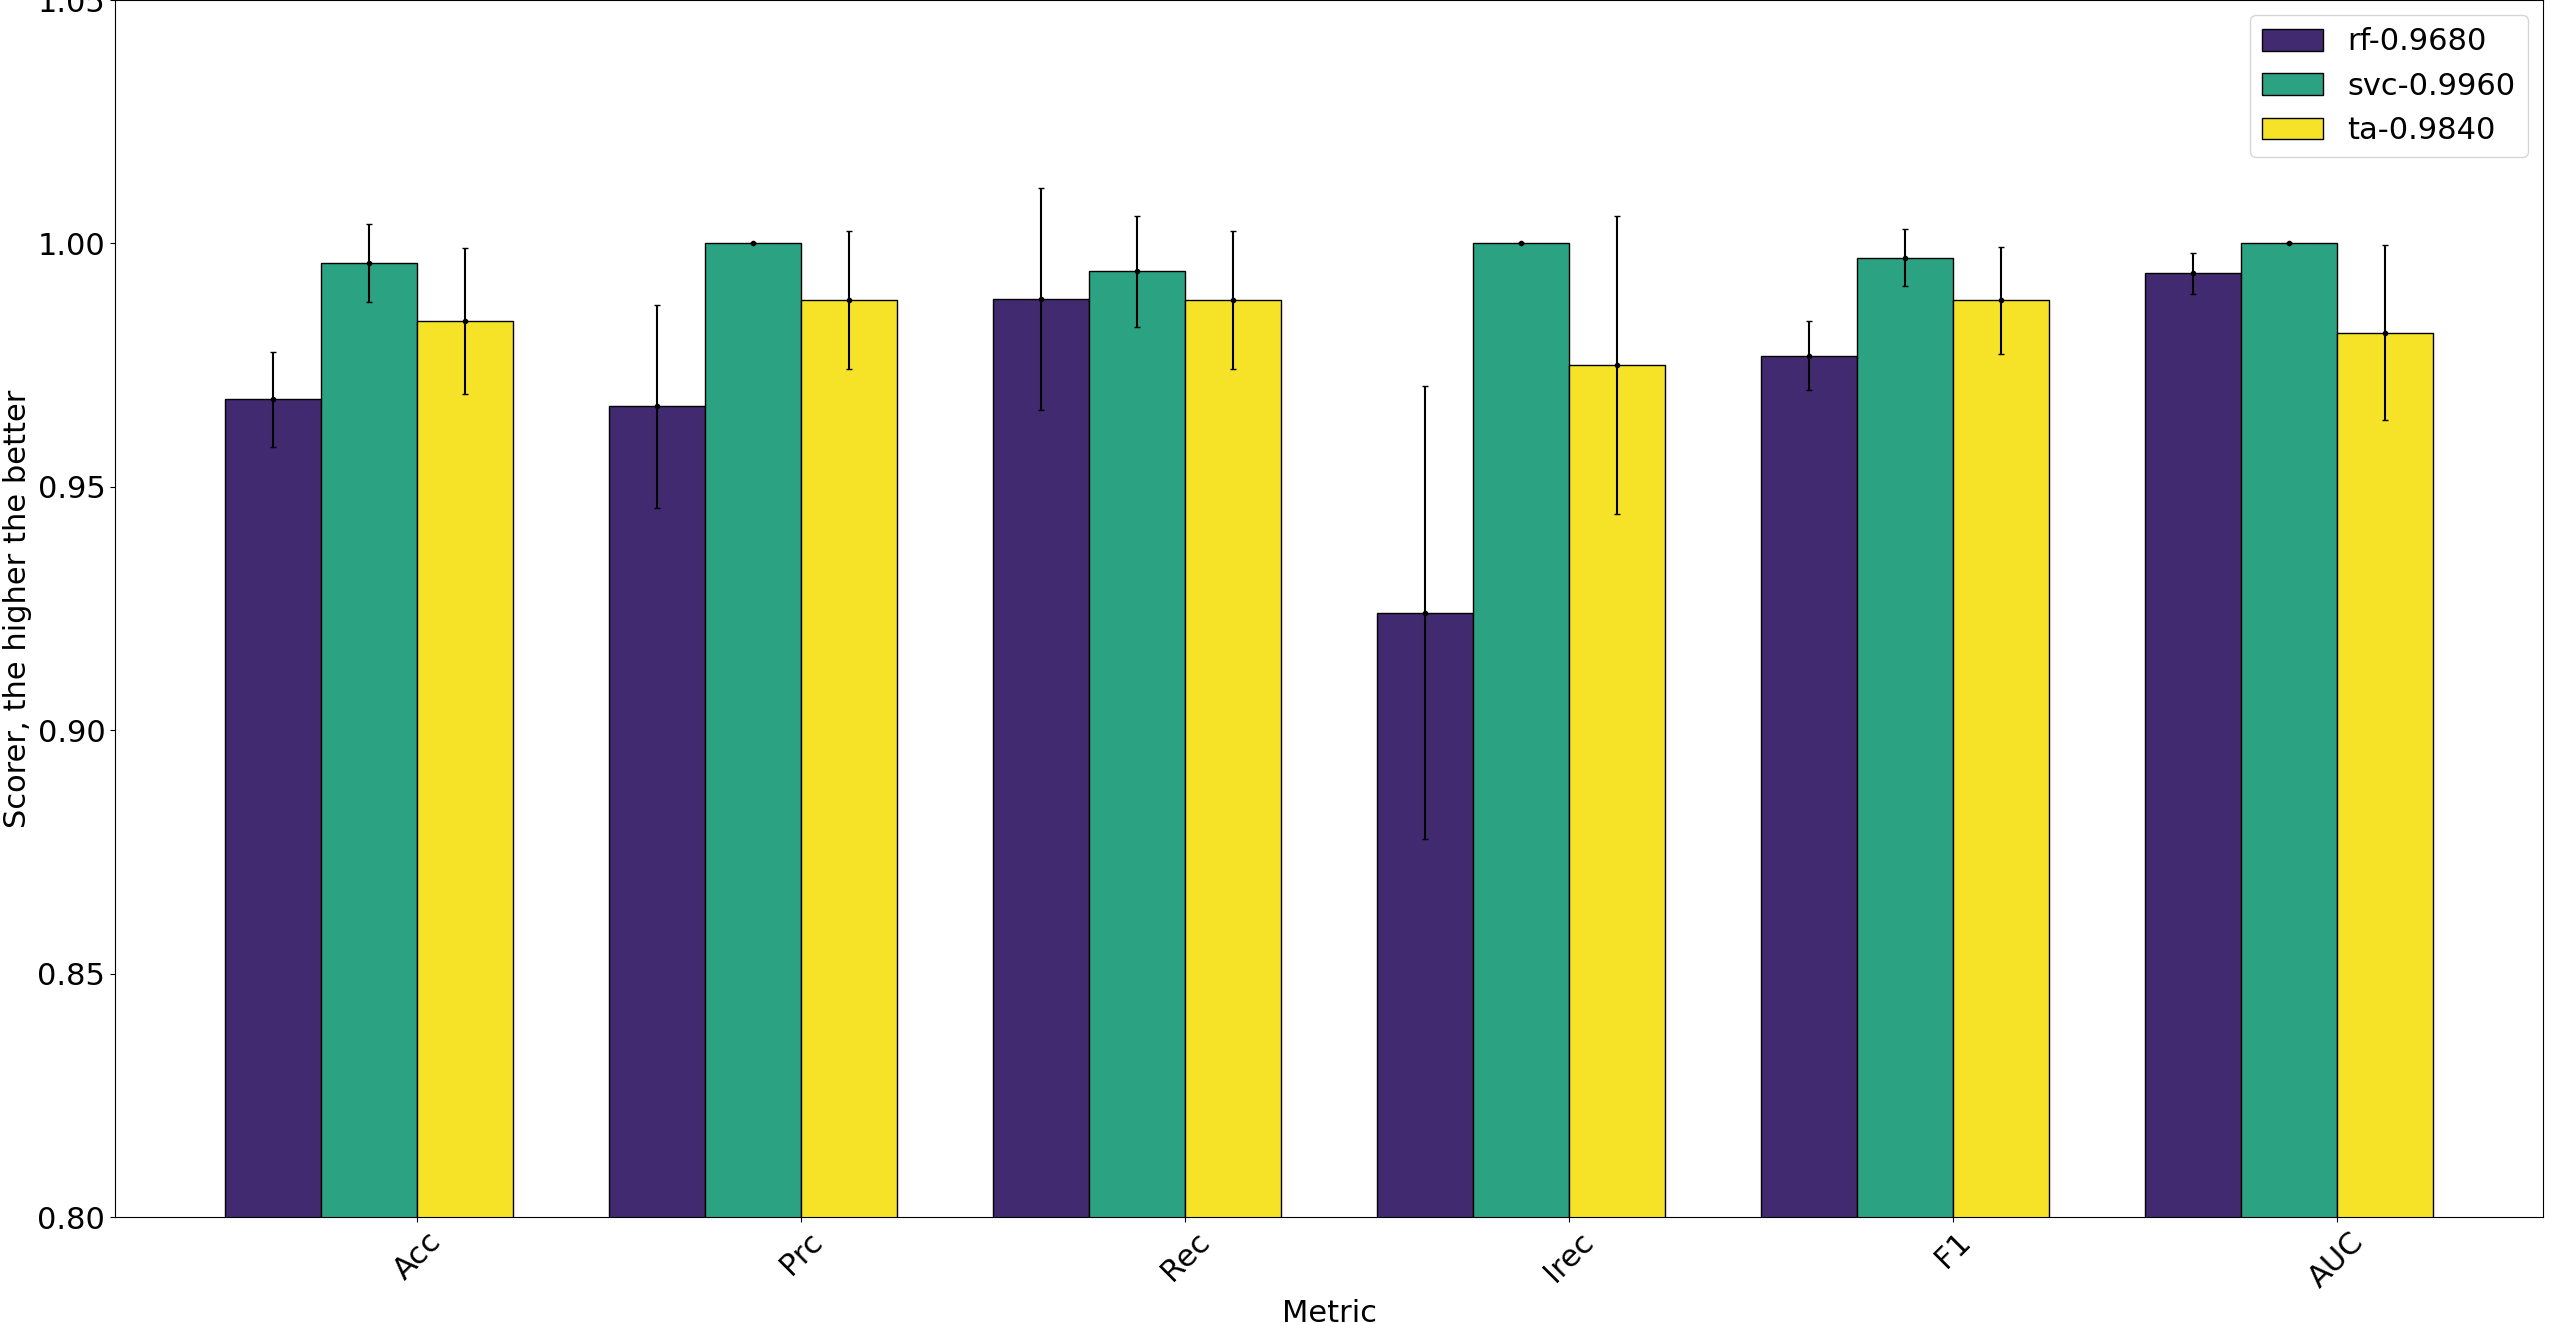
\includegraphics[width=\linewidth]{img/An_Cnmod_Phi_ta.png}
		\subcaption{\an, \cnmod, \phin}
	\end{subfigure}
	\begin{subfigure}{0.49\linewidth}
		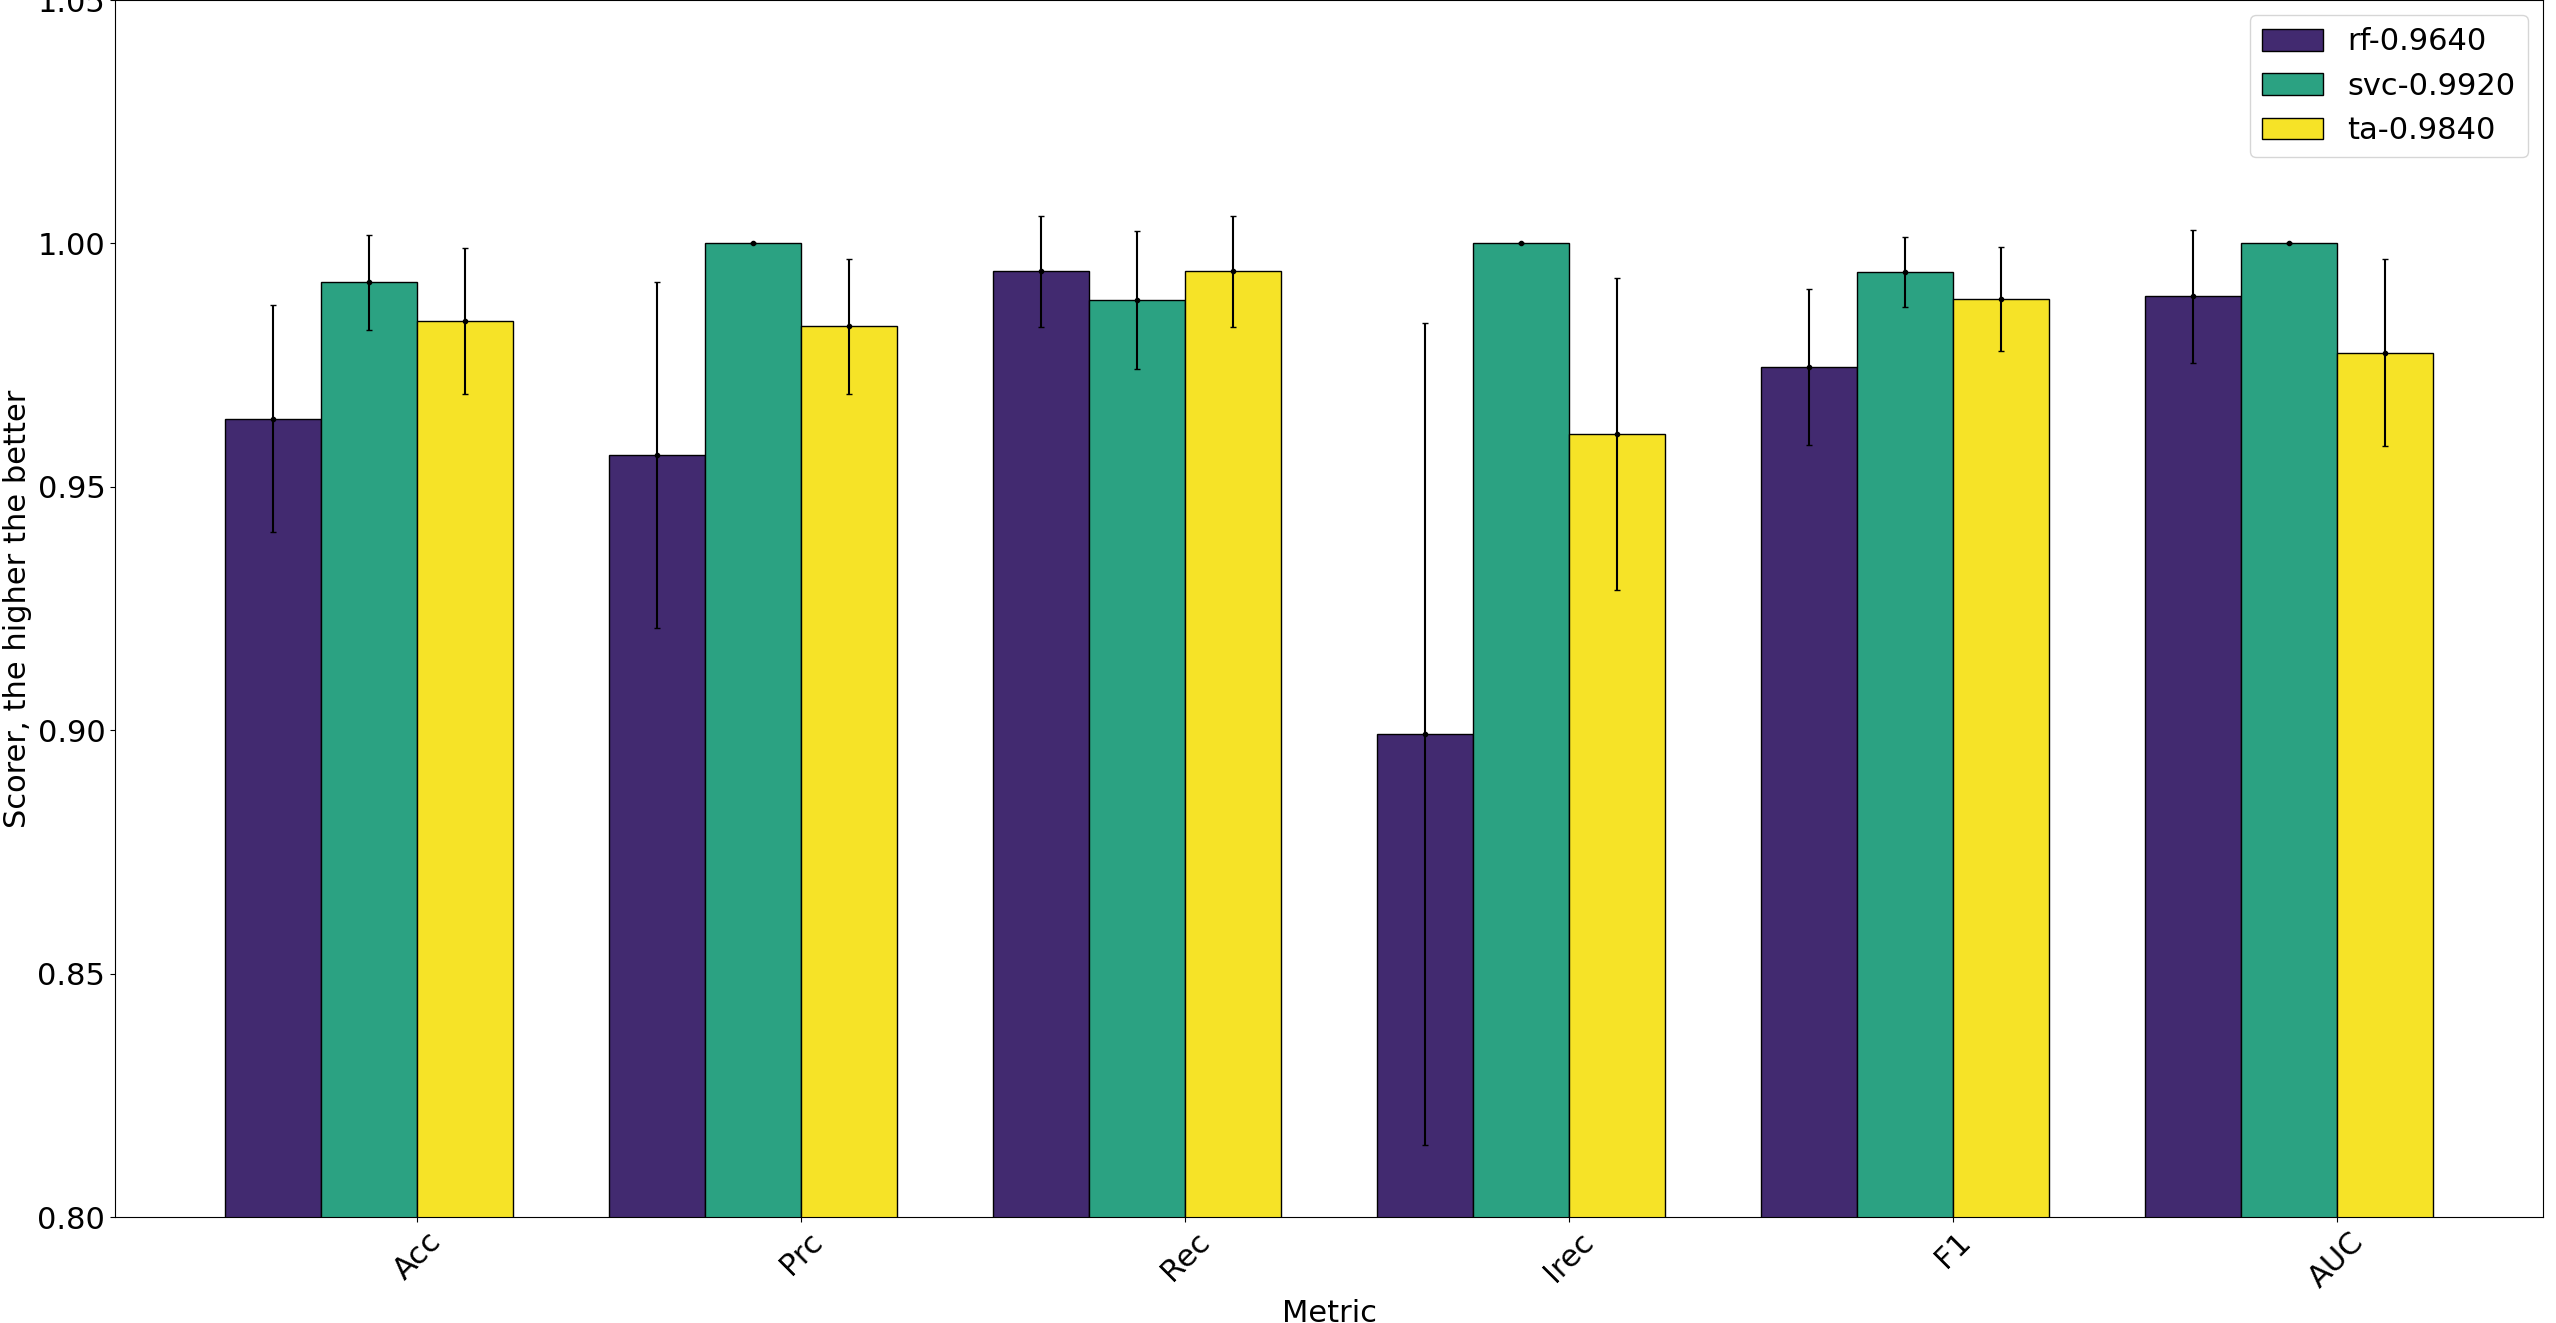
\includegraphics[width=\linewidth]{img/Bn_Cnmod_Phi_ta.png}
		\subcaption{\bn, \cnmod, \phin}
	\end{subfigure}
	\caption{Performance of \tas\ benchmarked against \rfs\ and \svcs, each model was trained on
		the same triplet to have an even testing ground.} \label{fig:triplets-performance}
\end{figure}
\begin{table}[!hb]
	\caption{Average and standard deviation of the \ta\ trained on the best sub-view for \an, \bn and
		\cnmod.}\label{tbl:an-bn-cnmod-ta-perf}

	\bigskip
	\setlength{\tabcolsep}{6pt}
	\centering
	\begin{tabular}{ccccccc}
		\toprule
		\textbf{}    & \textbf{Acc} & \textbf{Prc} & \textbf{Rec} & \textbf{Irec} & \textbf{F1} & \textbf{RAUC} \\
		\midrule
		Mean         & 0.996        & 1.0          & 0.994        & 1.0           & 0.997
		             & 0.997                                                                                    \\
		\textsc{std} & 0.008        & 0.0          & 0.011        & 0.0           & 0.006
		             & 0.006                                                                                    \\
		\bottomrule
	\end{tabular}
\end{table}
%Final scores for the model:
%accuracy -- avg: 0.9960   std: 0.0080
%precision -- avg: 1.0000   std: 0.0000
%recall -- avg: 0.9943   std: 0.0114
%inv-recall -- avg: 1.0000   std: 0.0000
%f1 -- avg: 0.9971   std: 0.0058
%roc_auc -- avg: 0.9971   std: 0.0057
The best aggregator was trained on \an, \bn\ and \cnmod, the model contains $3$ trees: one built
on a sub-view of \an, is shown in \Cref{fig:dt-an-2-12-pt}; the other two, one built on \bn, and one
built on \cnmod\footnote{
	While the best model originally found for \cnmod\ was trained on harmonics $\{2, 5, 13\}$
	(see \Cref{fig:best-dts}) the decision tree we used for the best \ta\ was trained on $\{3,
		4, 5, 14\}$, which has a lower accuracy. This was one of those instances in which
	the choice of greedily picking the \dt\ with the highest accuracy from storage does
	not pay off. This is why we chose to systematically avoid the first description in favor of
	the second.
}, are shown in \Cref{fig:part-of-bta}. Compared to the trees we described at the end
of the end of \Cref{sec:qrp-rf} they are a bit more complex: having depth between $4$ and $5$, which
is still very reasonable, while also having a larger volume of both internal nodes and leaves.

\Cref{fig:ta-rf-svc-comparison} compares the performance of the best: \ta\ (\an, \bn and \cnmod\ in
\Cref{fig:triplets-performance}), \rf\ and \svc. Once more, \ta\ performance are generally better
than \rf\ performance, except for ROC-AUC metric. Since both \ta\ and \rf\
predictions are aggregated via majority voting, we could explain this odd
behavior by highlighting that the forest contains more trees than the aggregator. Decisions could be slightly more biased in the case of \ta: in the first case we need
three estimators to obtain majority, while in the latter we only need two.
\begin{figure}[!ht]
	\centering
	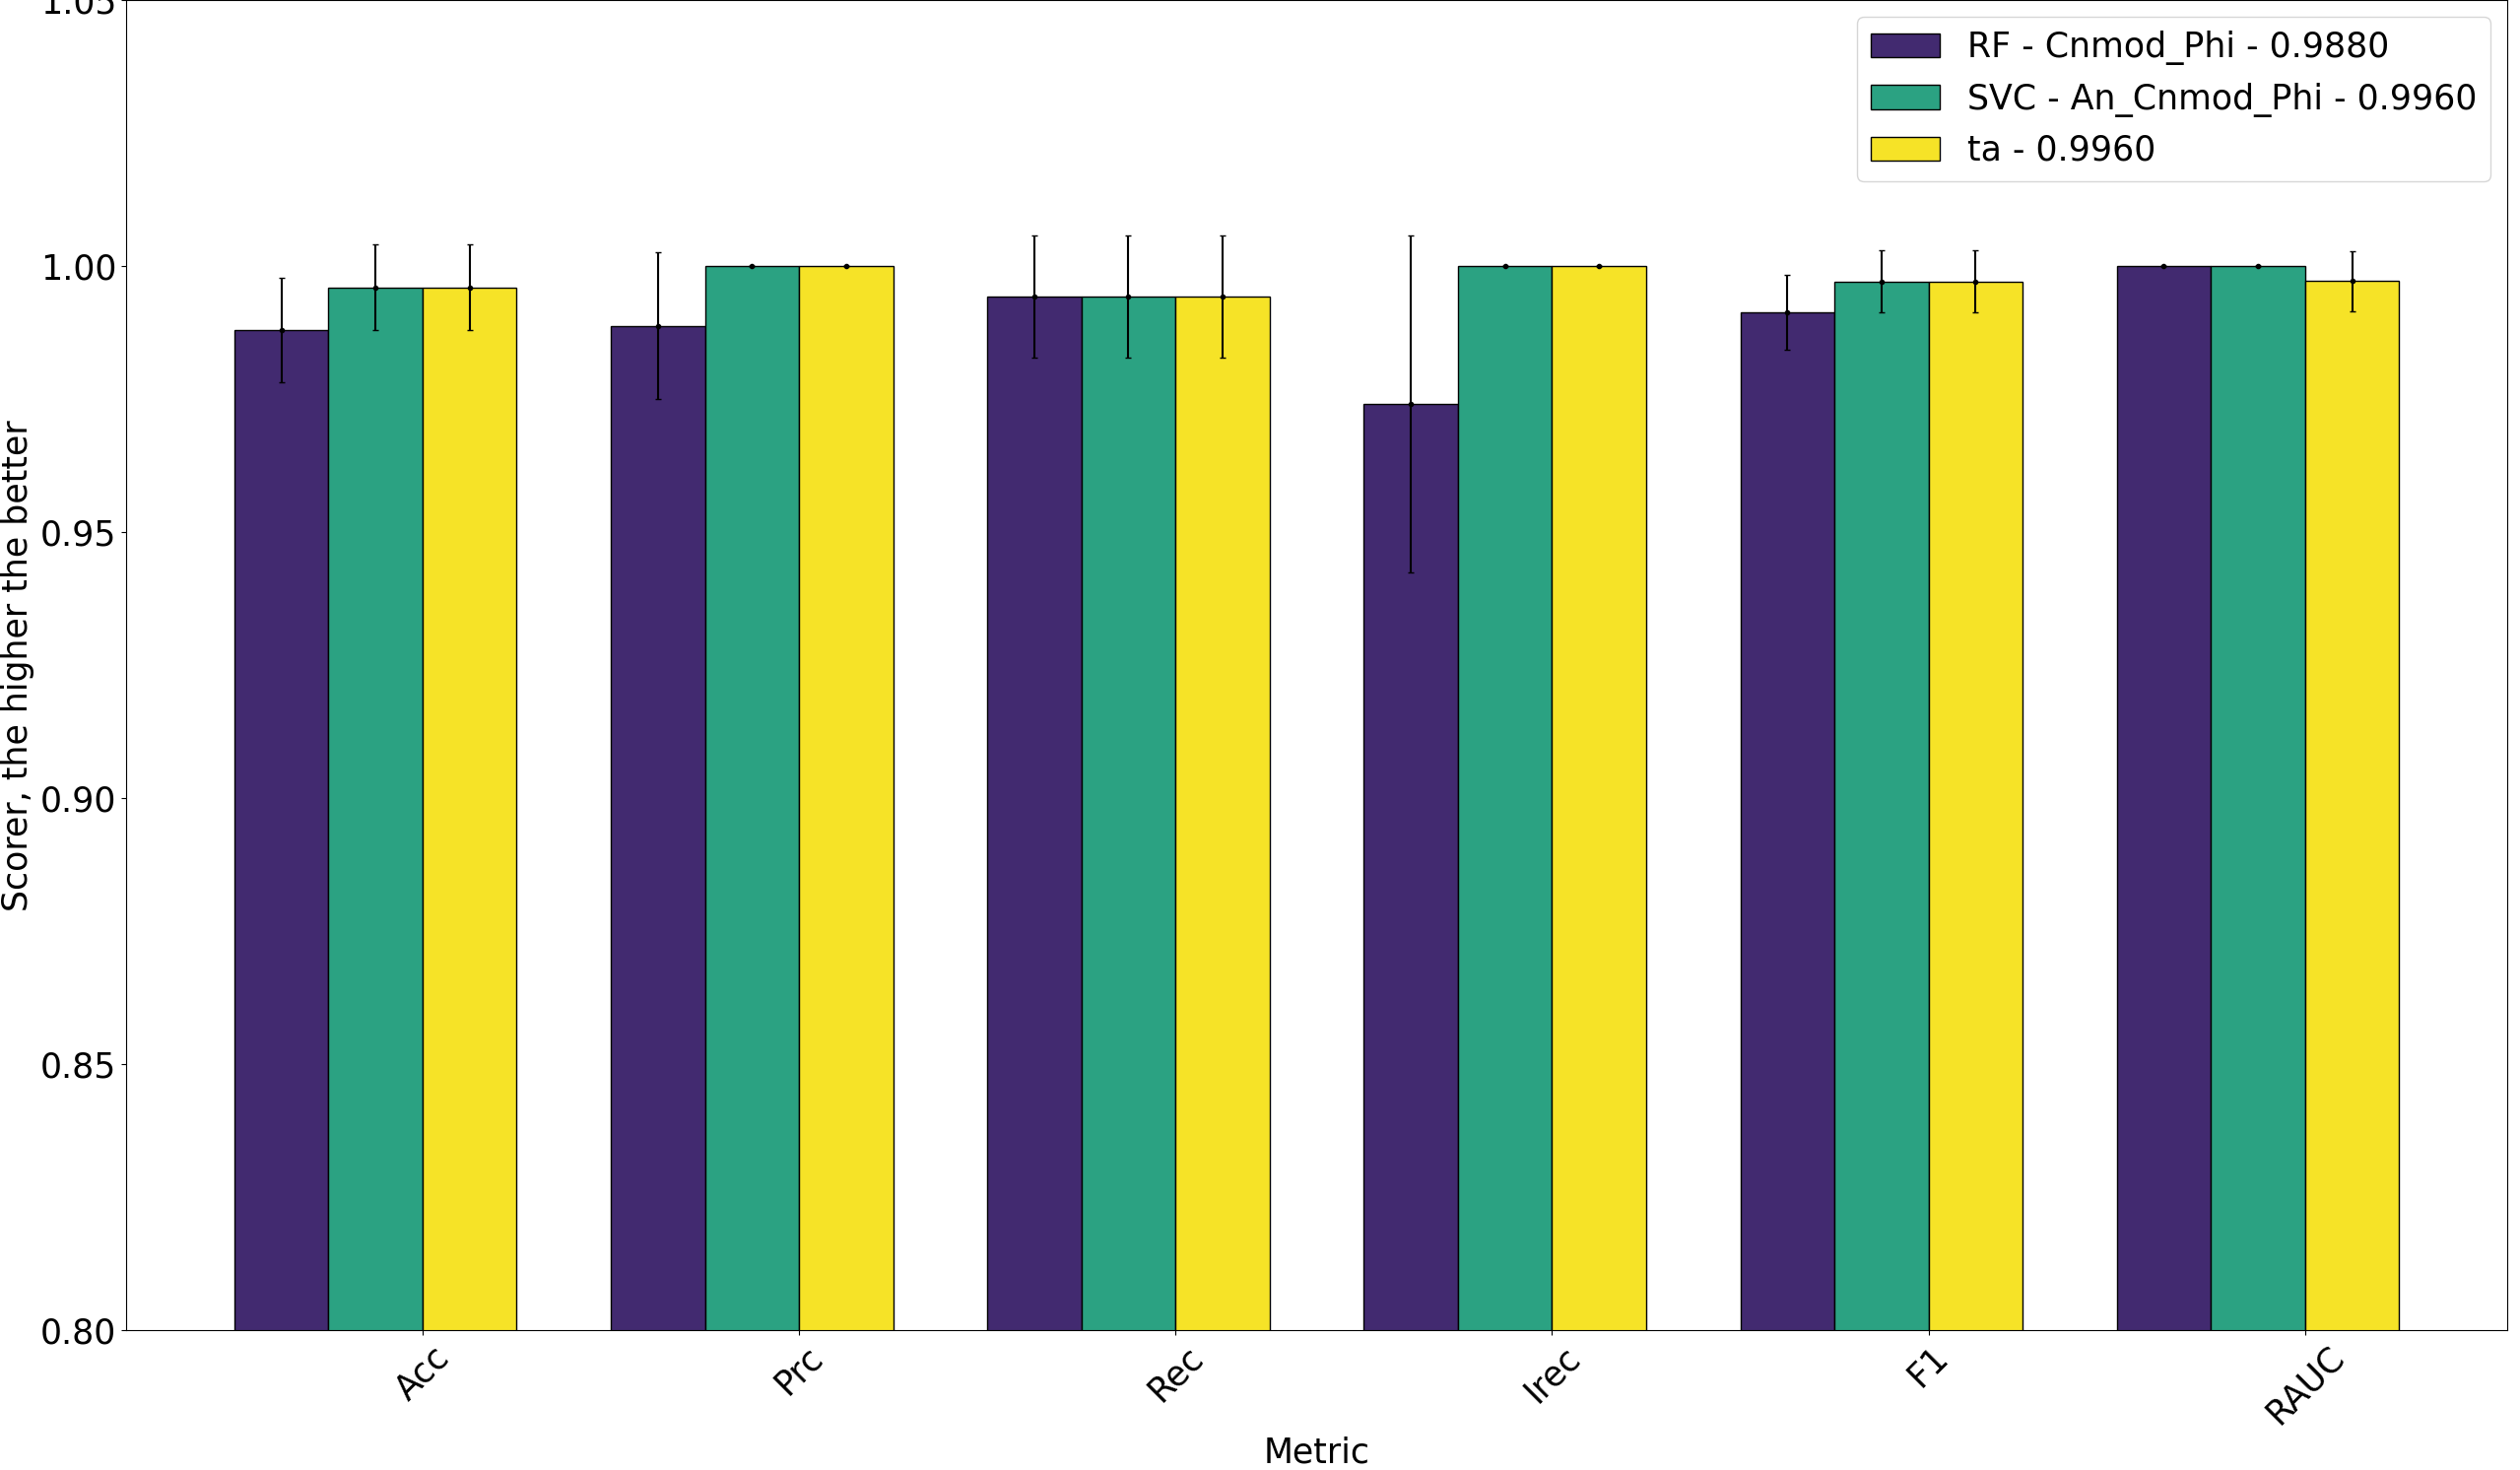
\includegraphics[width=\linewidth]{img/best_rf_ta_svc_compared.png}
	\caption{A performance comparison between the best \rf, the best \svc, and the best \ta,
		each of them trained on the sub-view of the original datasets the yields the best possible
		performance} \label{fig:ta-rf-svc-comparison}
\end{figure}

\begin{figure}[!ht]
	\centering
	\begin{subfigure}{\linewidth}
		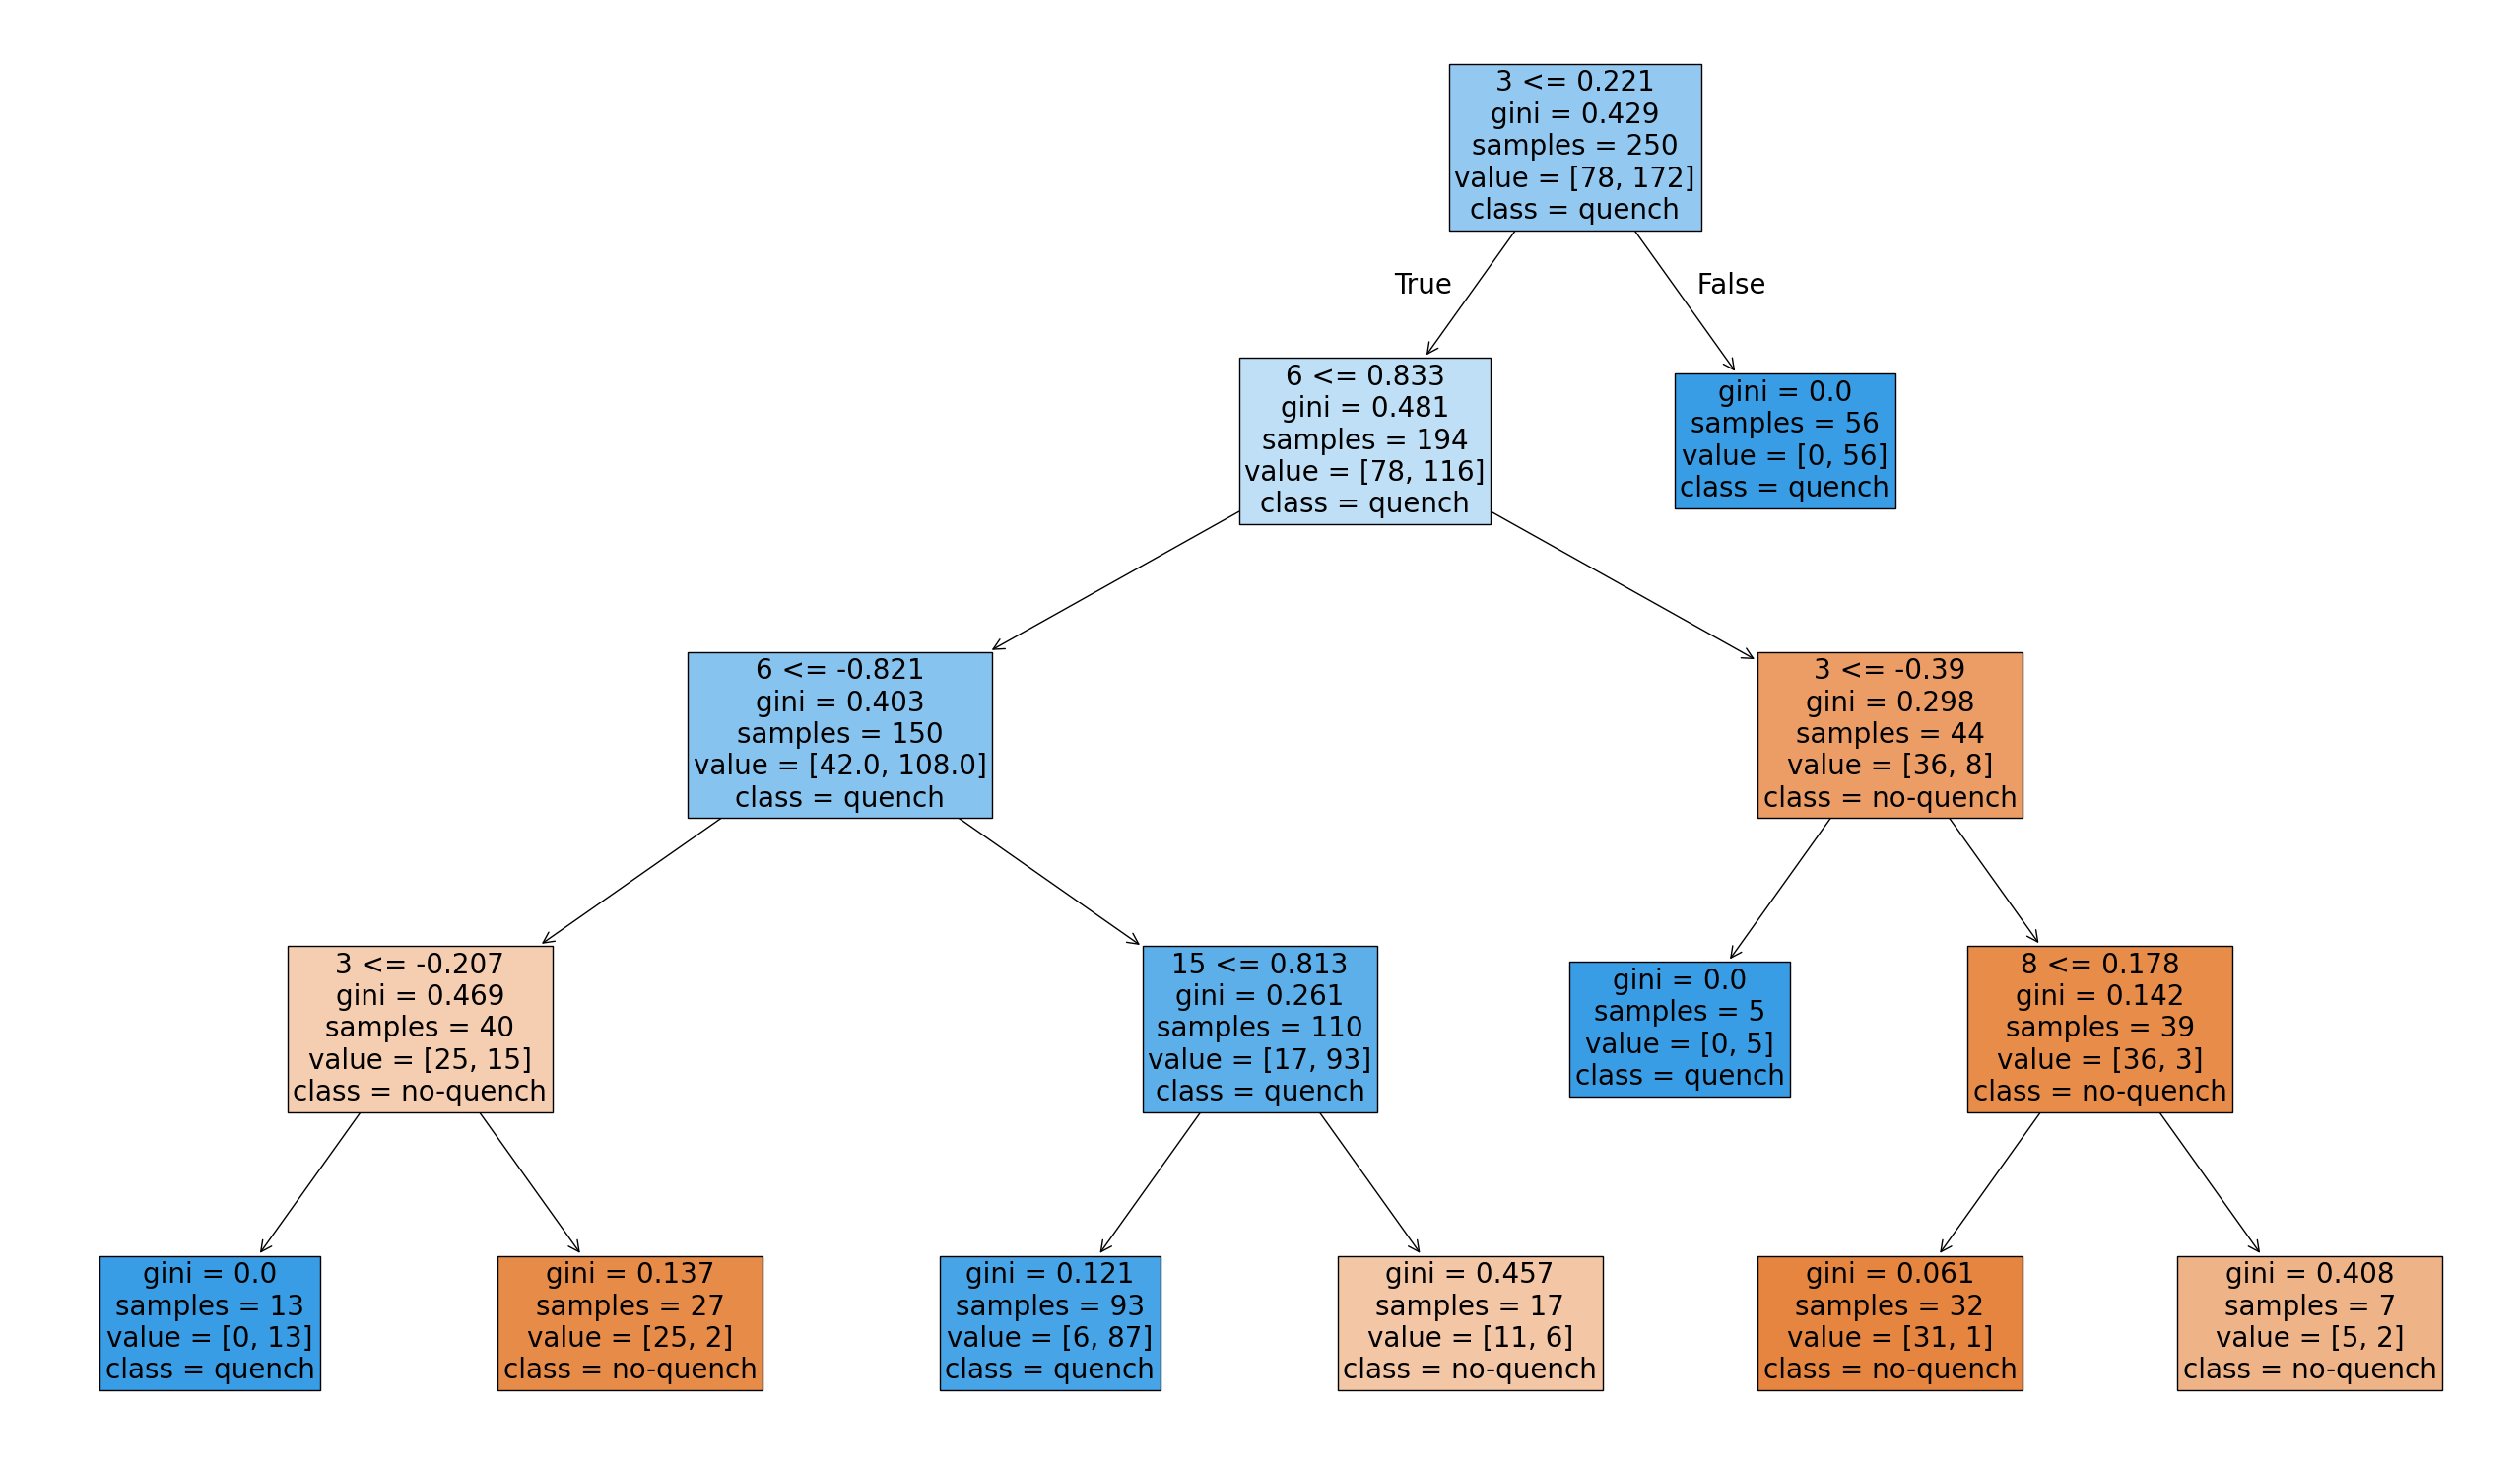
\includegraphics[width=\linewidth]{img/Bn_3_6_8_15_pt_dt.png}
		\subcaption{Tree trained on a subview of \bn}
	\end{subfigure}
	\begin{subfigure}{\linewidth}
		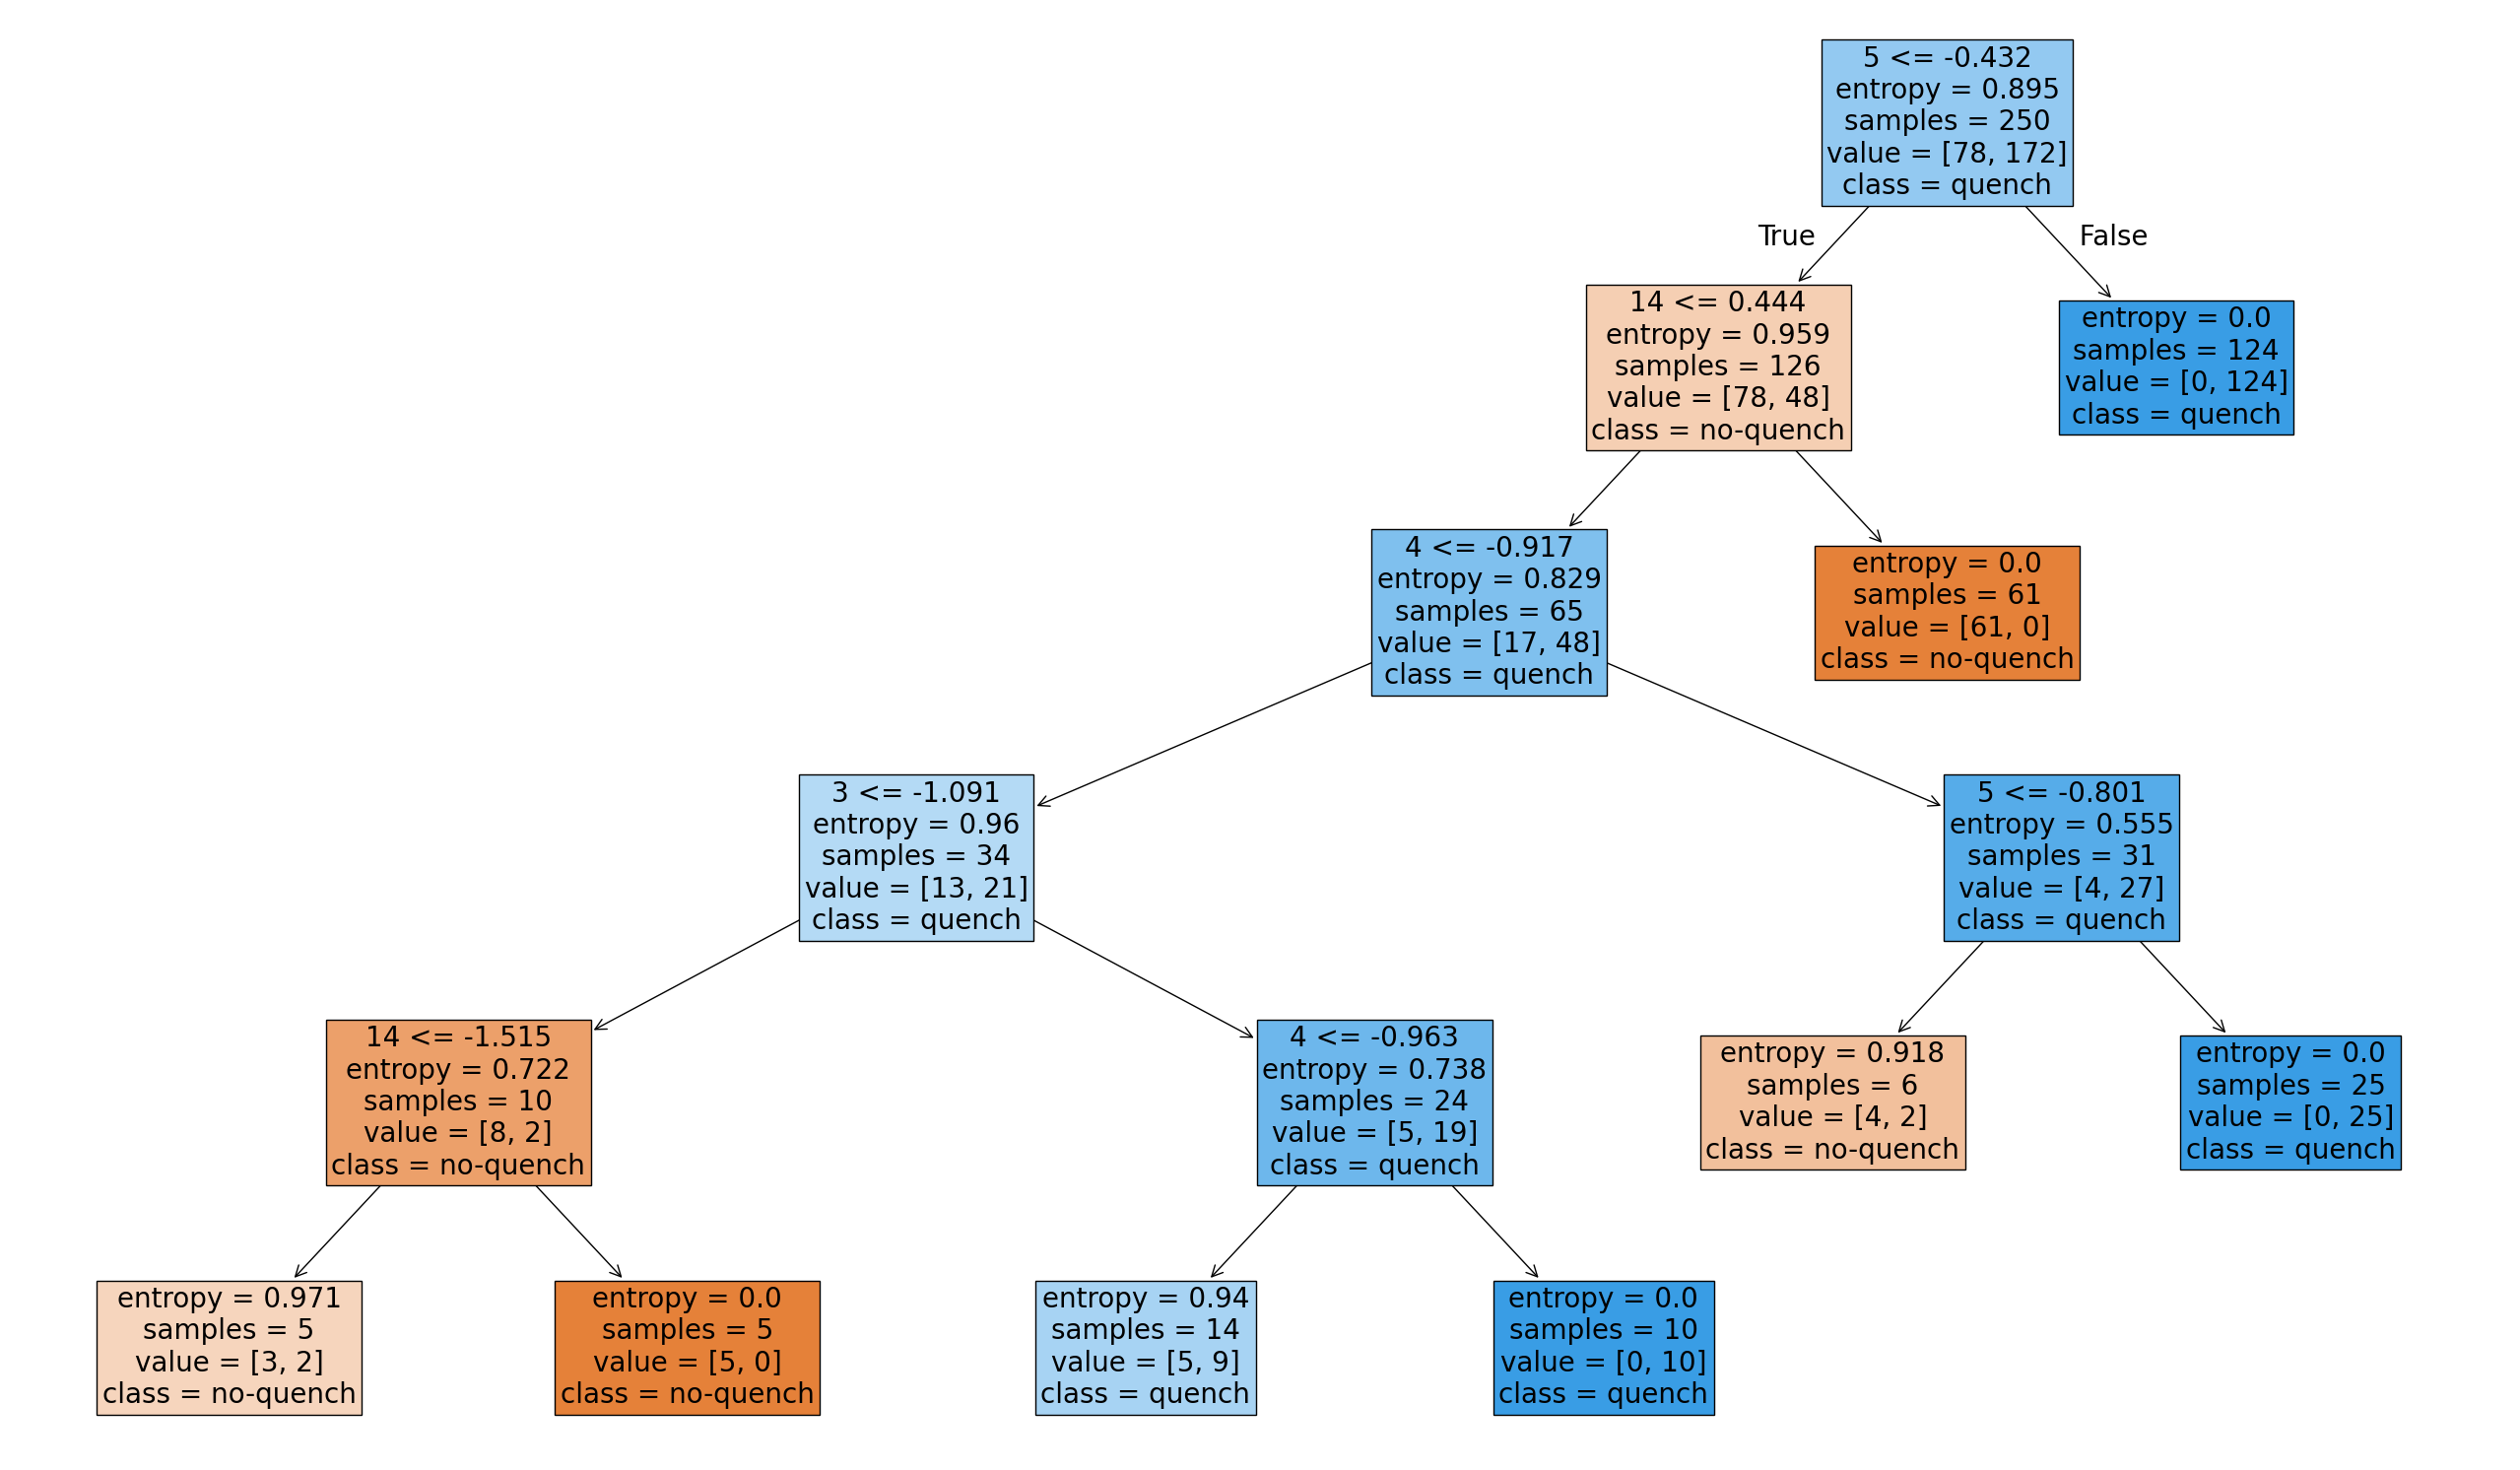
\includegraphics[width=\linewidth]{img/Cnmod_3_4_5_14_pt_dt.png}
		\subcaption{Tree trained on a subview of \cnmod}
	\end{subfigure}
	\caption{Two of the trees contained in the best \ta, the one trained on a subview of \an is
		shown in \Cref{fig:dt-an-2-12-pt}} \label{fig:part-of-bta}
\end{figure}

Finally, we evaluated the best \ta\ on the blind-test set \db, obtaining only an incorrect
classification over $29$ examples (precisely, a false positive), corresponding to the metric values
detailed in Table \Cref{tbl:qrp-ta-test}, essentially confirming our initial estimate.

\begin{table}[!ht]
	\caption{Performances of the best TA on the blind test set $\mathscr
			D_\mathrm{test}$.}\label{tbl:qrp-ta-test}

	\bigskip
	\setlength{\tabcolsep}{6pt}
	\centering
	\begin{tabular}{cccccc}
		\toprule
		\textbf{Acc} & \textbf{Prc} & \textbf{Rec} & \textbf{F1} & \textbf{Irec} & \textbf{RAUC} \\
		\midrule
		0.965        & 0.952        & 1            & 0.976       & 0.889         & 0.944         \\
		\bottomrule
	\end{tabular}
\end{table}

\subsection{Final considerations on \qrp}
In this chapter we have introduced the problem of \qrp: we showed different models and we
chose the best estimator for each class (\dt, \rf\ and \ta). In each subsection we have
highlighted the strengths, weaknesses and characteristics of the classifiers found, and we provided the
results of a final blind-test. We have now a good reason to believe that the \ta\ is better than the
alternatives because of the very high performance and simplicity.

If we had to declare an alternative we would indicate the Decision tree as the best backup due to
the relatively strong performance compared to the extremely simple architecture (only $7$ nodes and
$\approx 0.984$ accuracy). To compare, the best \rf\ reaches similar numbers but contains $5$
different trees.








\chapter{Quench Localization Problem (\qlp)}
\label{chp:qlp}
This chapter is dedicated to some initial results for the Quench Localization Problem (\qlp), we will discuss:
\begin{inparaenum}[(i)]
	\item some of the preprocessing we have done, specific for the labels,
	\item some preliminary results obtained by clustering, and finally,
	\item the results obtained, just like we did in \Cref{sec:results-qrp}
\end{inparaenum}.
\section{Data preprocessing}
\label{sec:qlp-preprocessing}
As we said in \Cref{chp:problem}, the main difference between \qlp\ and \qrp\ is the number of
classes. While \qrp\ is a binary classification problem, \qlp\ is a multiclass-classification
problem. As was already stated in \Cref{chp:problem}, the expected outcome is a $4$ bit binary array, each of the bits represents the state of one of the coils in the magnet ($1$ if the coil quenched, $0$ if it is in normal working conditions). In this section, we will concentrate on the considerations arisen from the analysis of the new labels, and the visualization of the samples in bidimensional space.

\subsubsection{\an}
\Cref{fig:an-lcorr-qlp} shows the correlation with the labels, \an\ is correlated very strongly with
coils $0$ and $2$, but is less suited to explain the behavior of coils $1$ and $3$. If we remind
ourselves of the correlation existing among the harmonics, originally shown in \Cref{fig:an-corr}, we can see that:
\begin{itemize}
	\item Contrarily to what we discovered in \Cref{sec:qrp-preprocessing}, \an[2]\ is not
	      fundamental to explain the expected results;
	\item The harmonics containing more information are the odd ones (\an[1], \an[3], \an[5],
	      \ldots). This means that we will be able to only take one from the bunch, due to the
	      strong correlation among odd-numbered harmonics (cfr. \Cref{fig:an-corr}).
\end{itemize}
A potential dataset could be constructed using a primary odd harmonic (like \an[1]\ or \an[3]), the
harmonic performing the best among \an[4], \an[8]\ and \an[12]\ (which are all strongly correlated,
cfr. \Cref{fig:an-corr}), and finally, \an[2]\ and another high-order harmonic could be beneficial. Due to
the very low correlation between the \an\ harmonics and the labels for coil $1$ and $3$ we didn't really
consider it as an attribute worth exploring.
\begin{figure}[!ht]
	% Font size = 70
	\centering
	\begin{subfigure}{0.49\linewidth}
		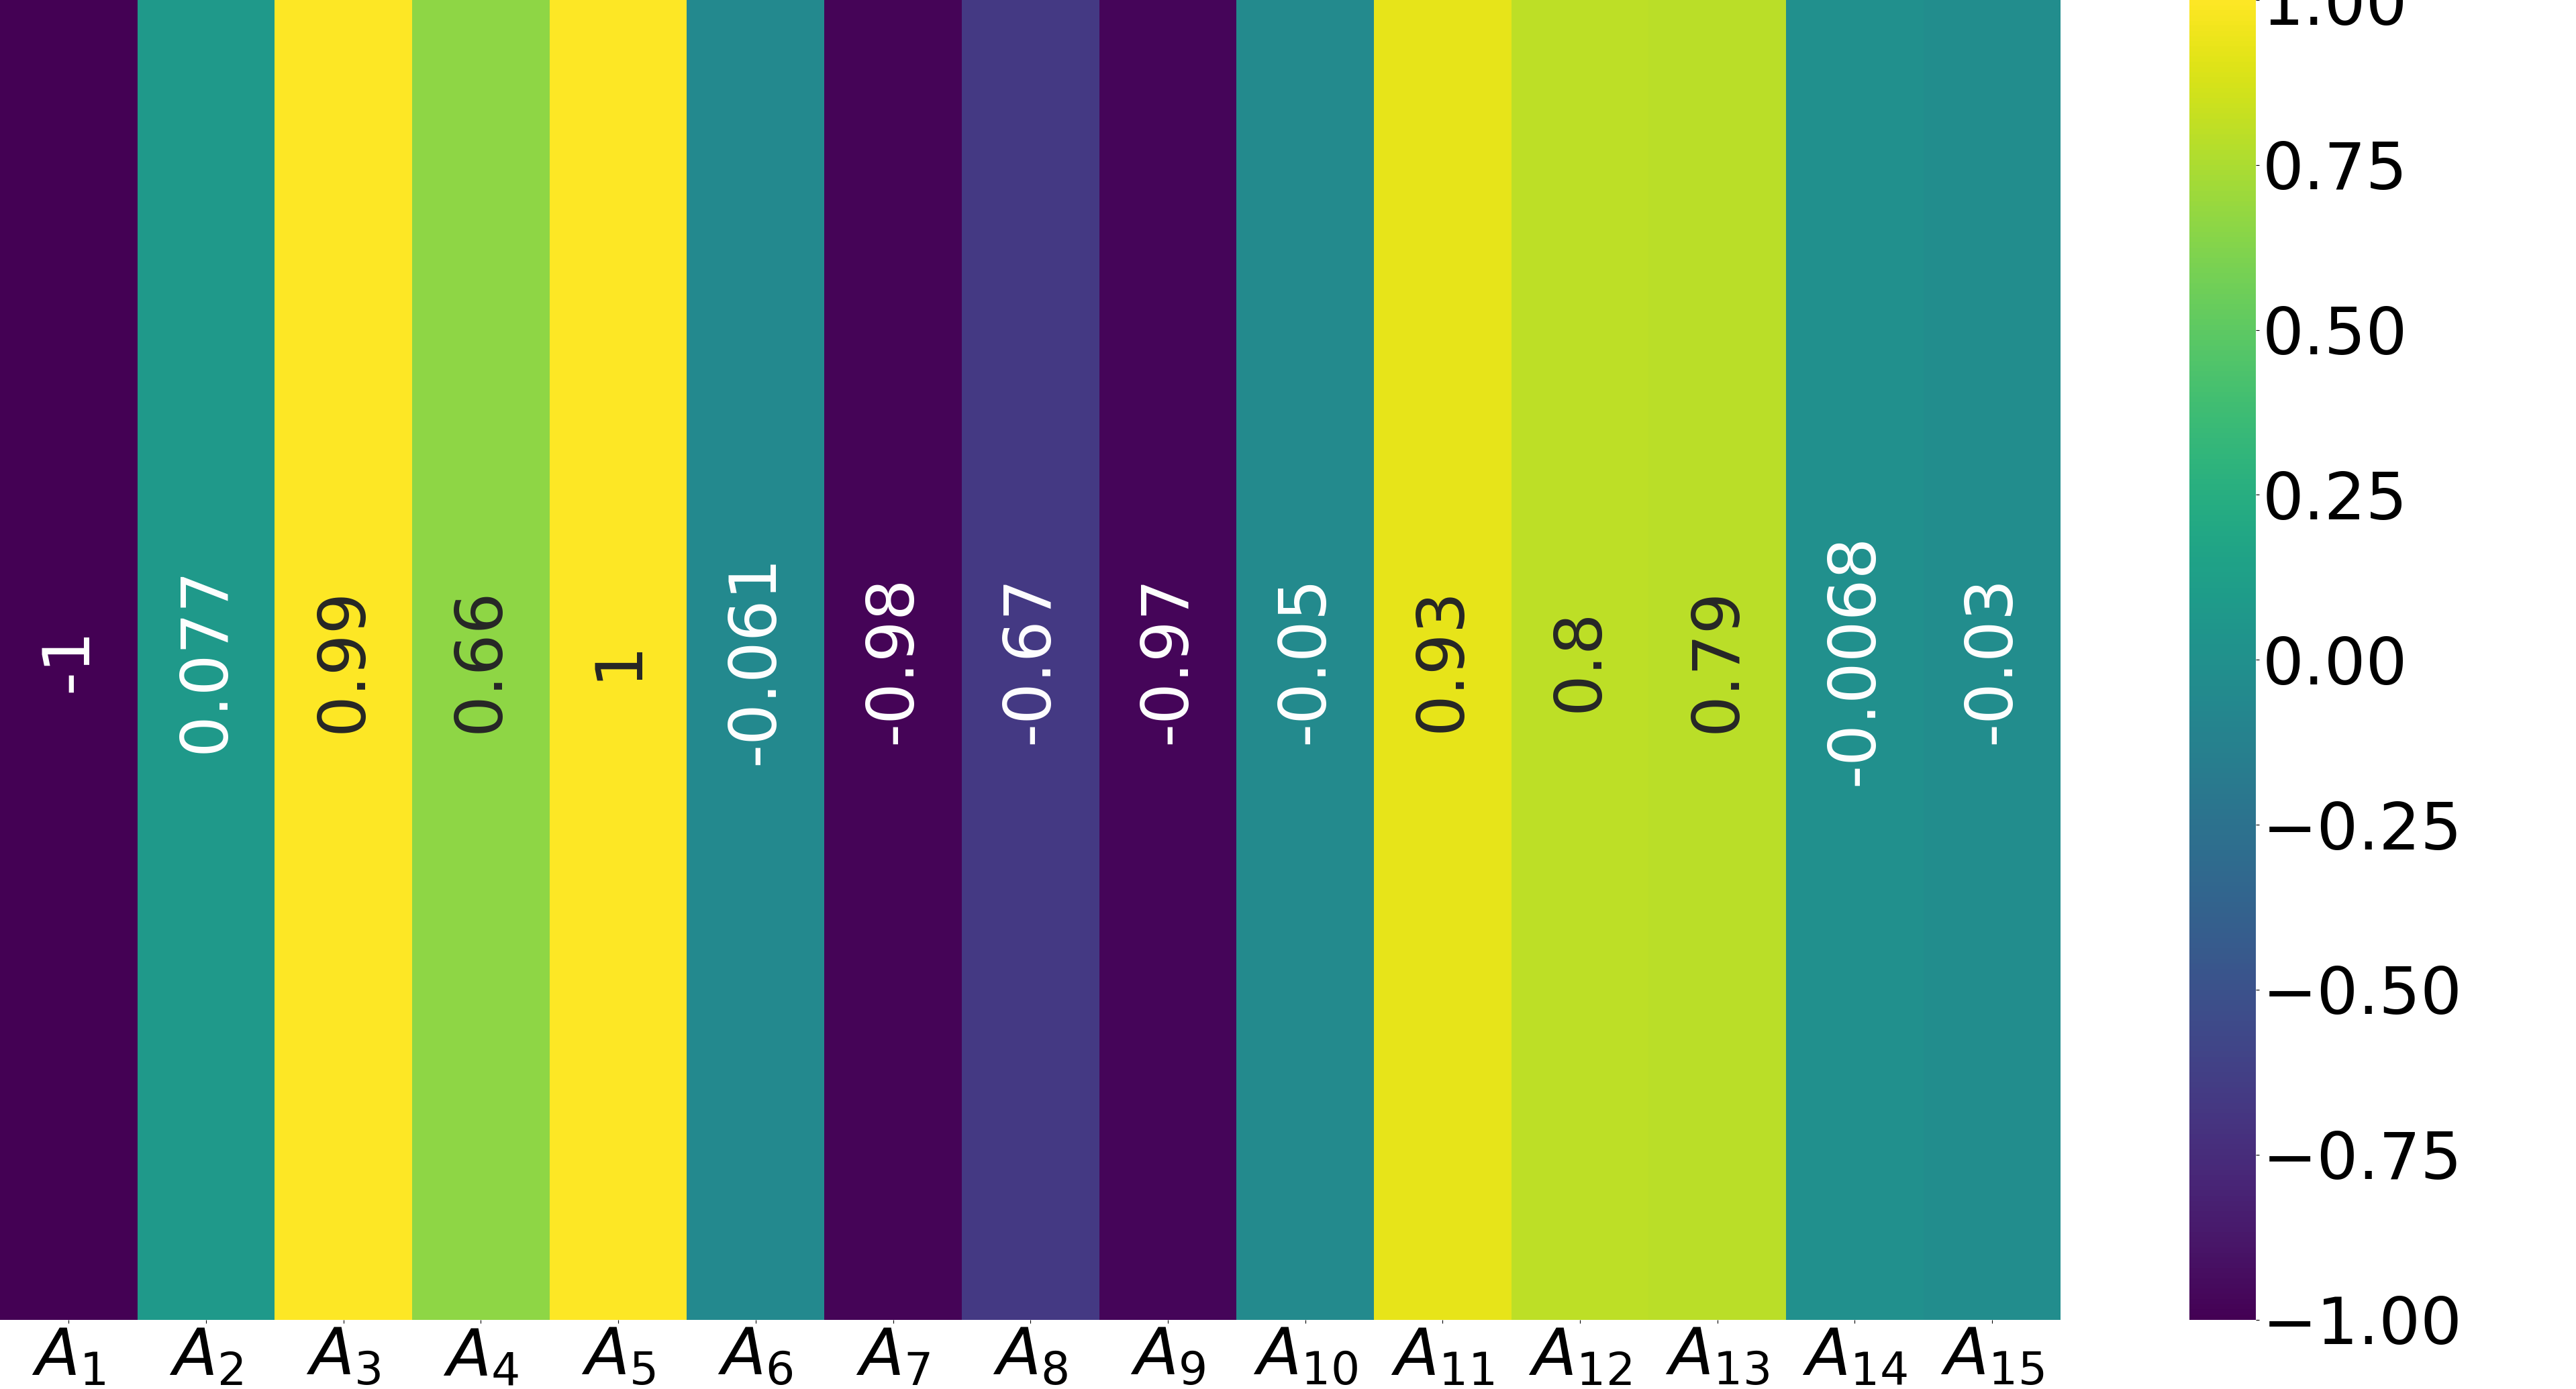
\includegraphics[width=\linewidth]{img/qlp_corr/An_coil0.png}
		\subcaption{Correlation with coil $0$}
	\end{subfigure}
	\begin{subfigure}{0.49\linewidth}
		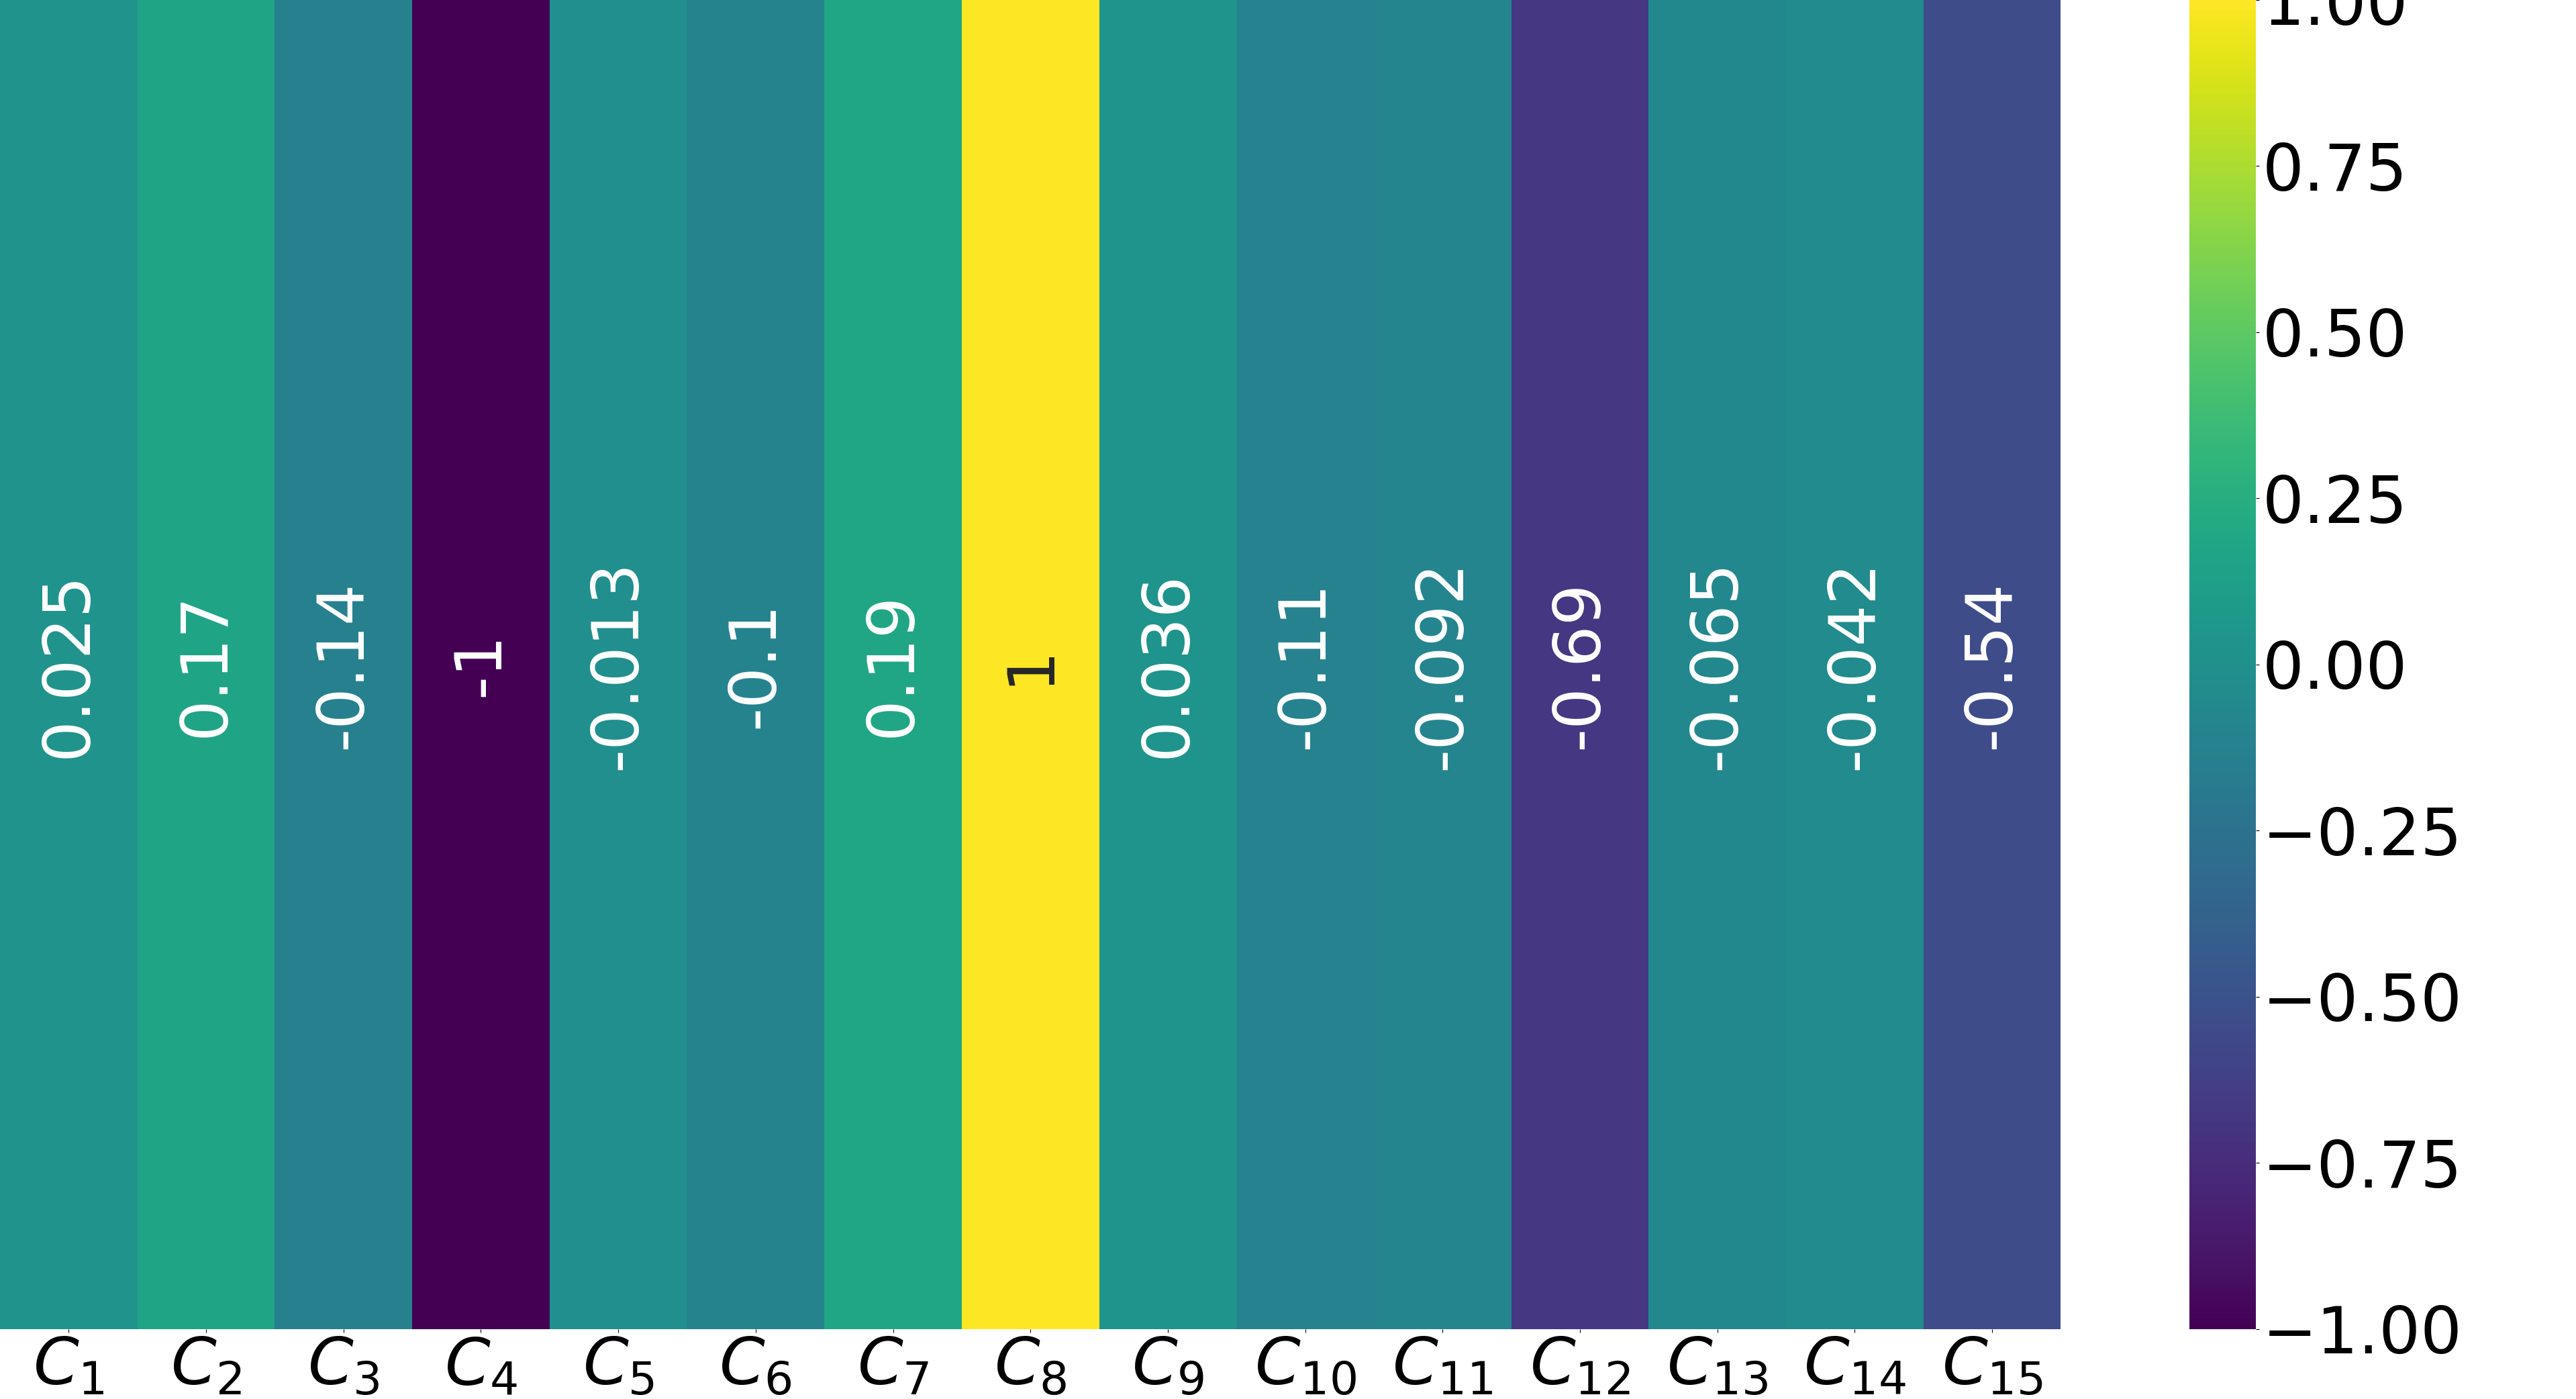
\includegraphics[width=\linewidth]{img/qlp_corr/An_coil1.png}
		\subcaption{Correlation with coil $1$}
	\end{subfigure}
	\begin{subfigure}{0.49\linewidth}
		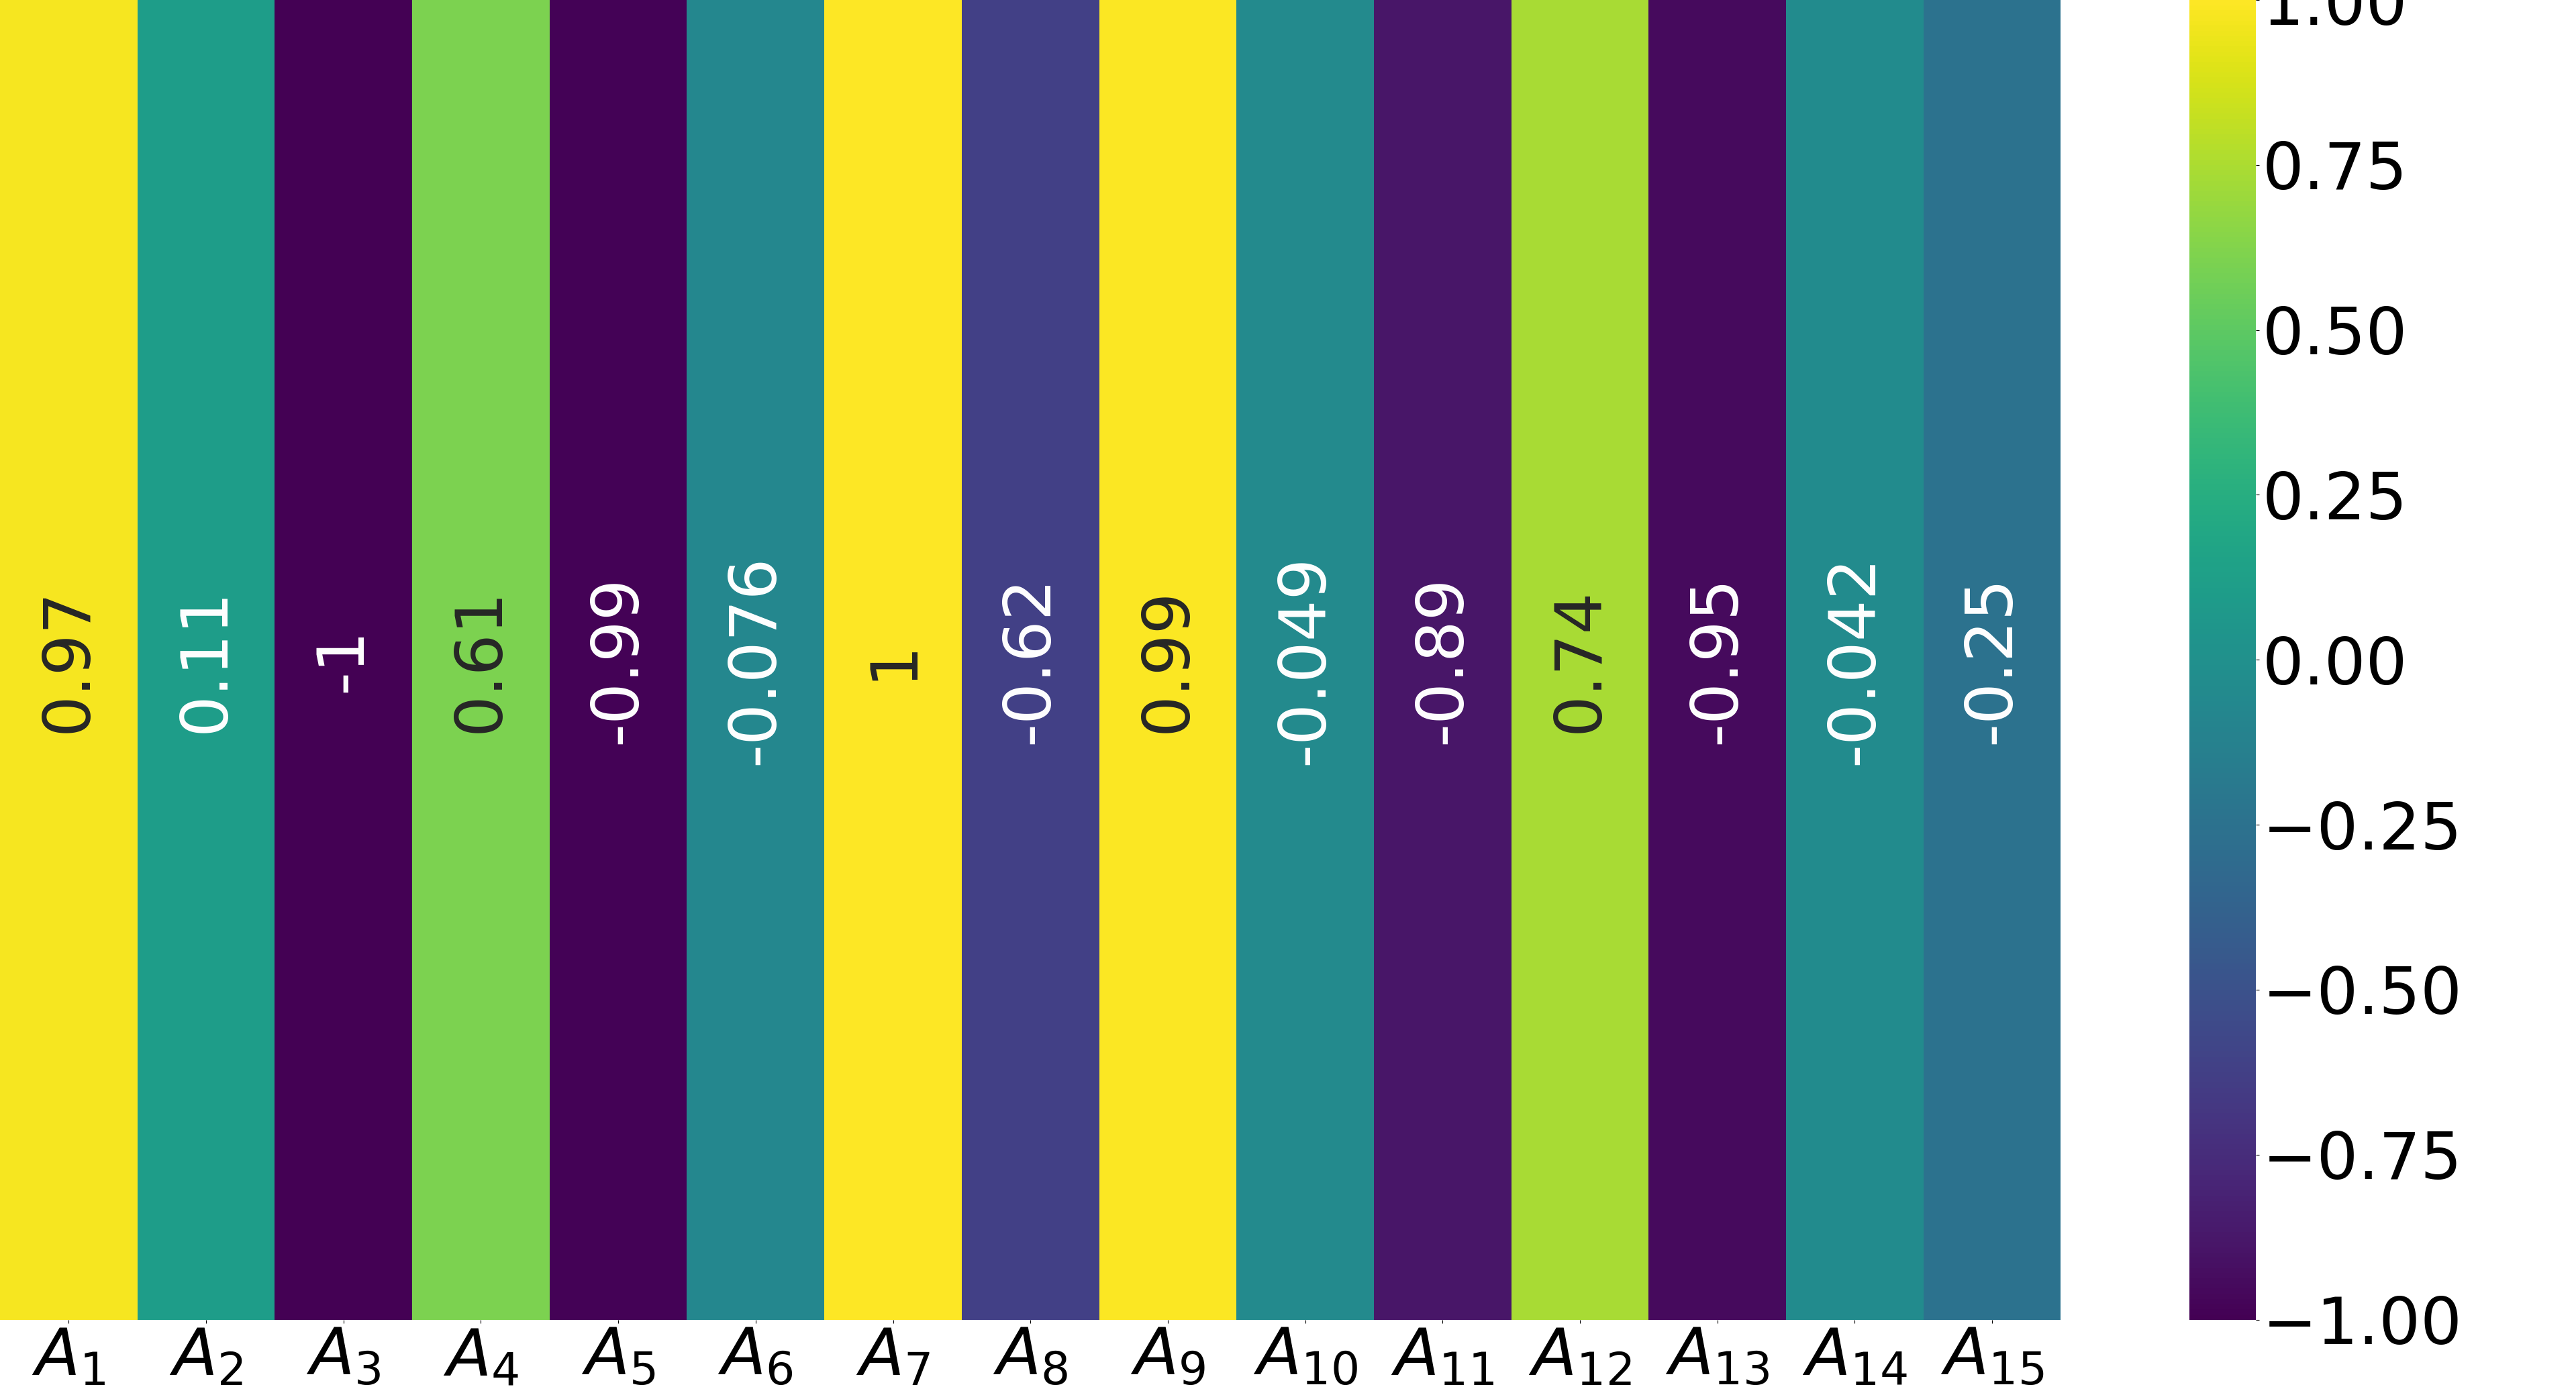
\includegraphics[width=\linewidth]{img/qlp_corr/An_coil2.png}
		\subcaption{Correlation with coil $2$}
	\end{subfigure}
	\begin{subfigure}{0.49\linewidth}
		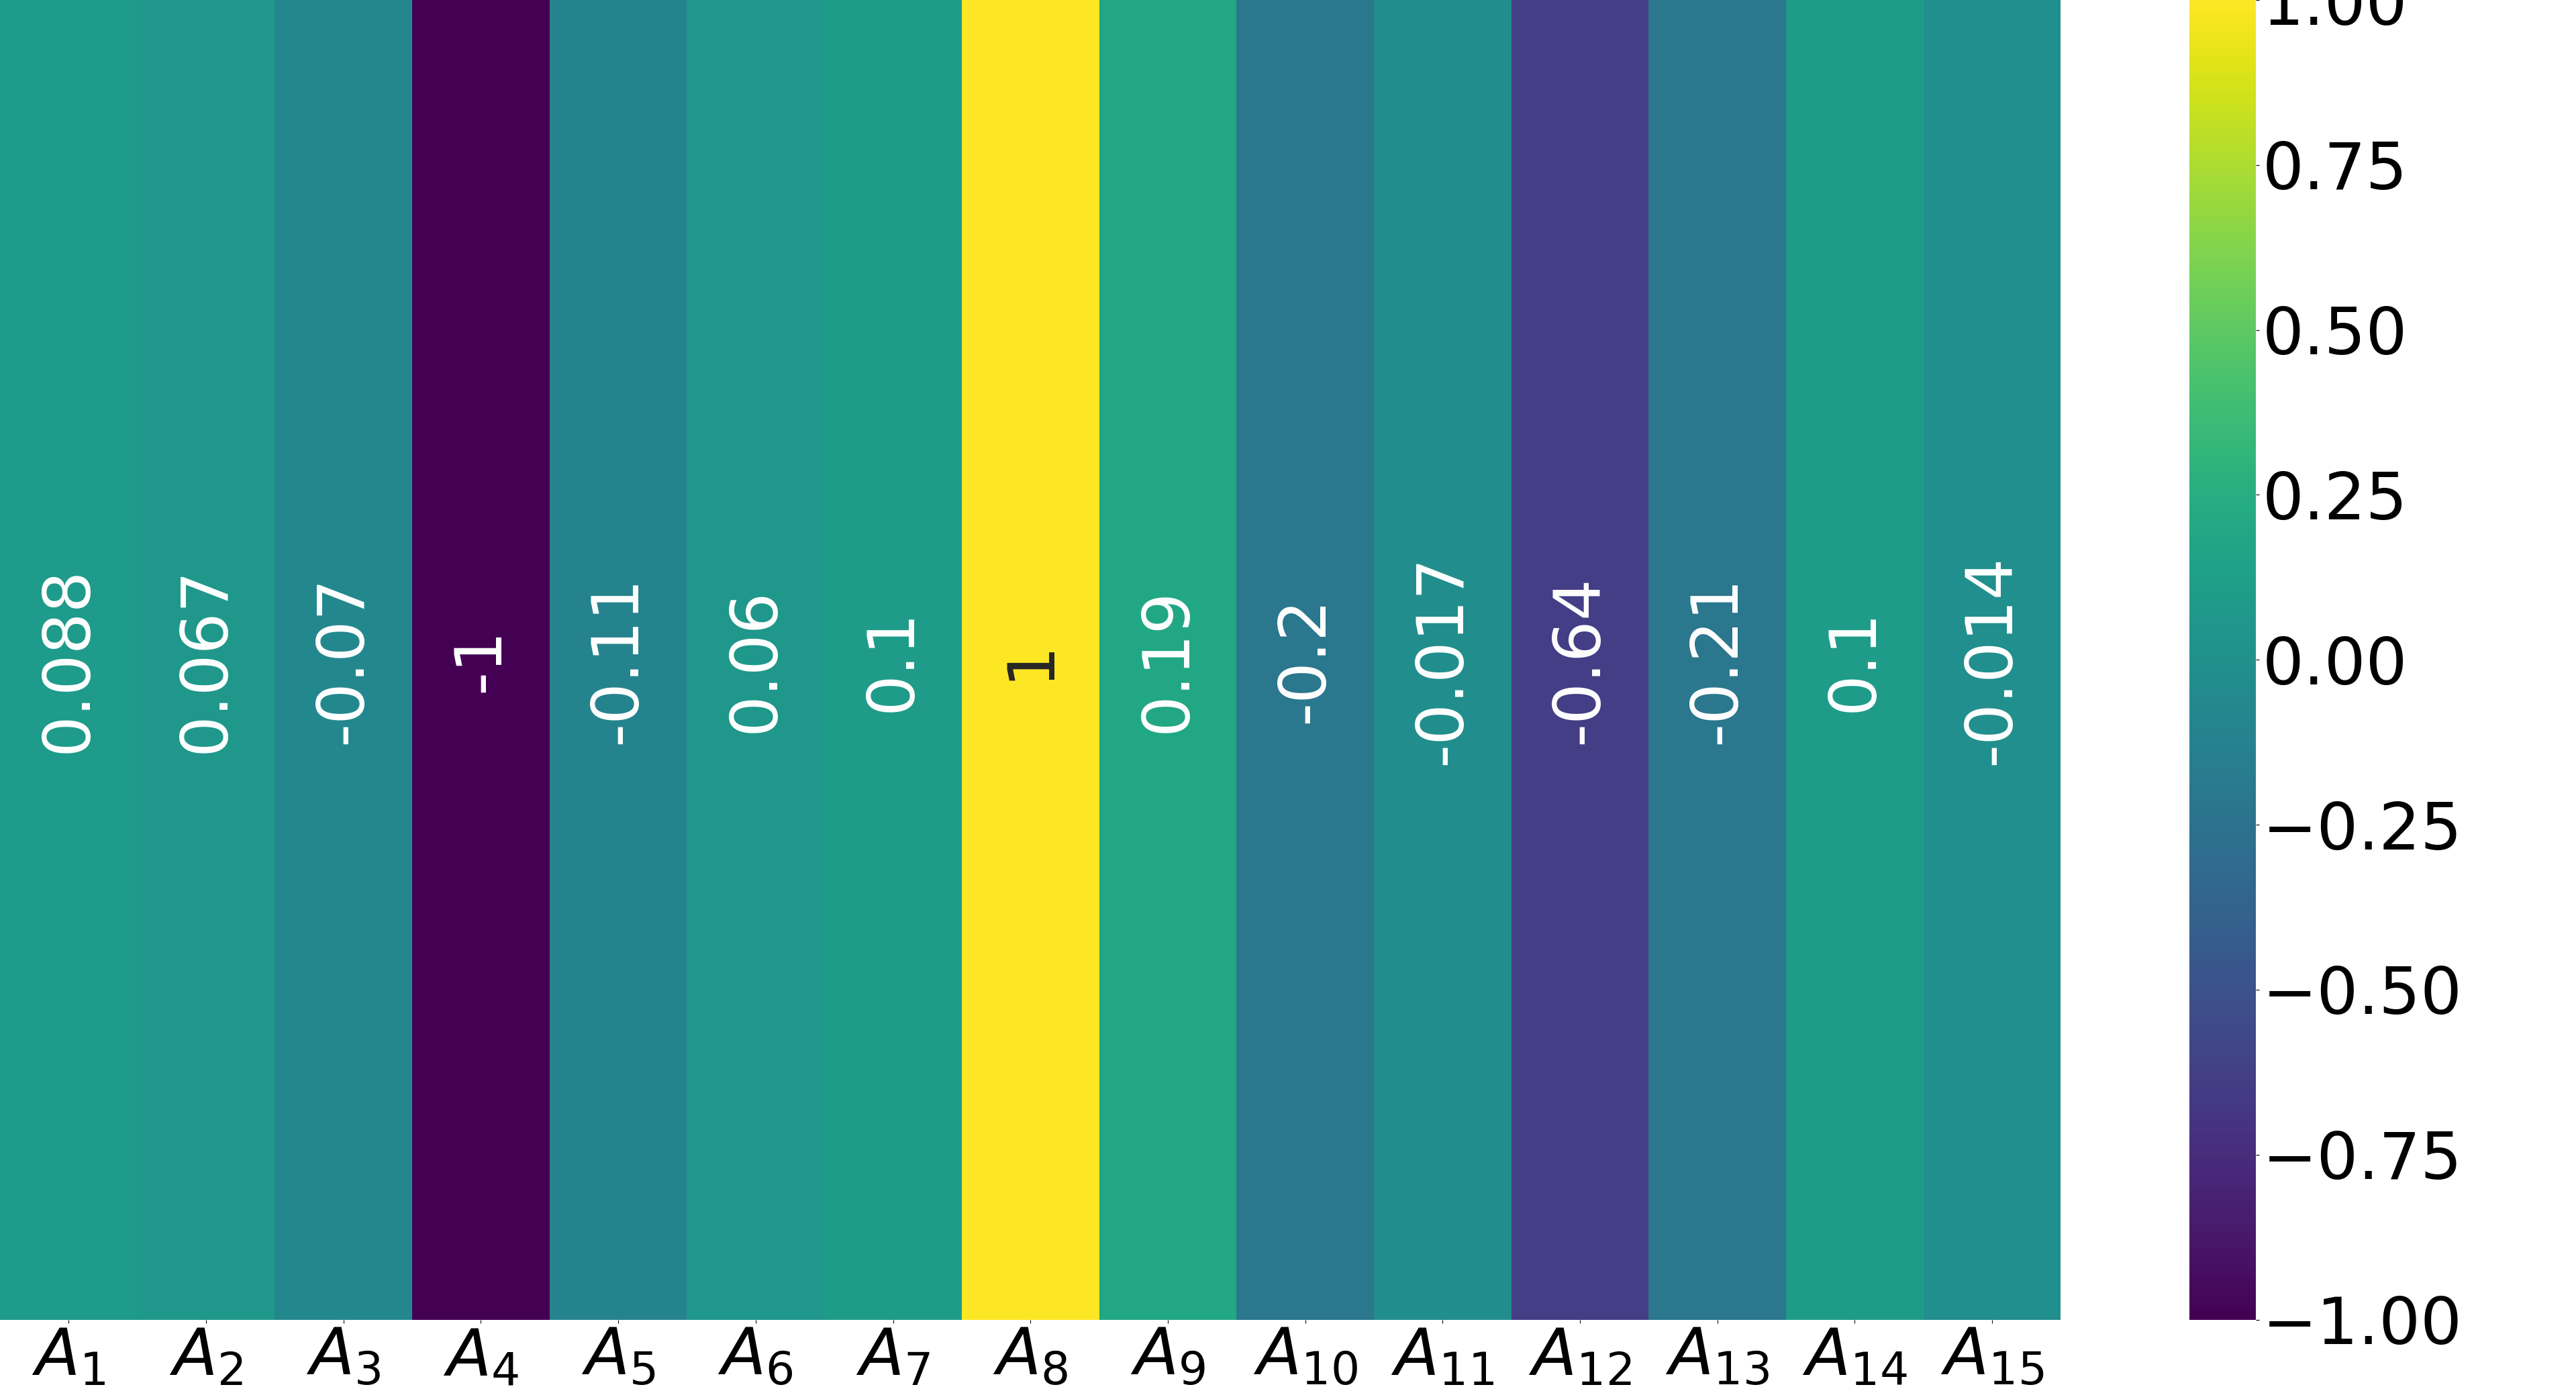
\includegraphics[width=\linewidth]{img/qlp_corr/An_coil3.png}
		\subcaption{Correlation with coil $3$}
	\end{subfigure}
	\caption{Correlation between the harmonics of the \an\ attribute and the labels for \qlp.}
	\label{fig:an-lcorr-qlp}
\end{figure}

In figure \Cref{fig:an-coilq-dist} we visualized the distribution of samples for \an\ in
bidimensional space, after a round of \pca\ dimensionality reduction (moving from $15$ to $2$
dimensions). Sub-figure (a) labels data based on the number of quenched coils associated to the
sample. We can evidently identify a series of clusters, characterized by a high degree of purity, in
\Cref{sec:qlp-cluster} we are going to discuss the clustering approach on this specific attribute.
In sub-figure (b), we labelled the data based on which coil was quenched. The division of the labels
is not as neat as in sub-figure (a), which lead us to think that clustering could be used as a
preprocessing step to then have another machine learning model work on the clustered data to
predict quench localization.

While sub-figure (b) doesn't tell us everything we need to know, we can see that coil $1$ and coil
$3$ are fairly mixed together, furthermore both of them are usually involved in multi-coil quenches.
These hints are giving us another possible reason why the attribute is less-than-ideal to
predict quench localization on coils $3$ and $1$ \Cref{fig:an-lcorr-qlp}.

\begin{figure}[!ht]
	% Font size = 40
	\centering
	\begin{subfigure}{0.8\linewidth}
		\centering
		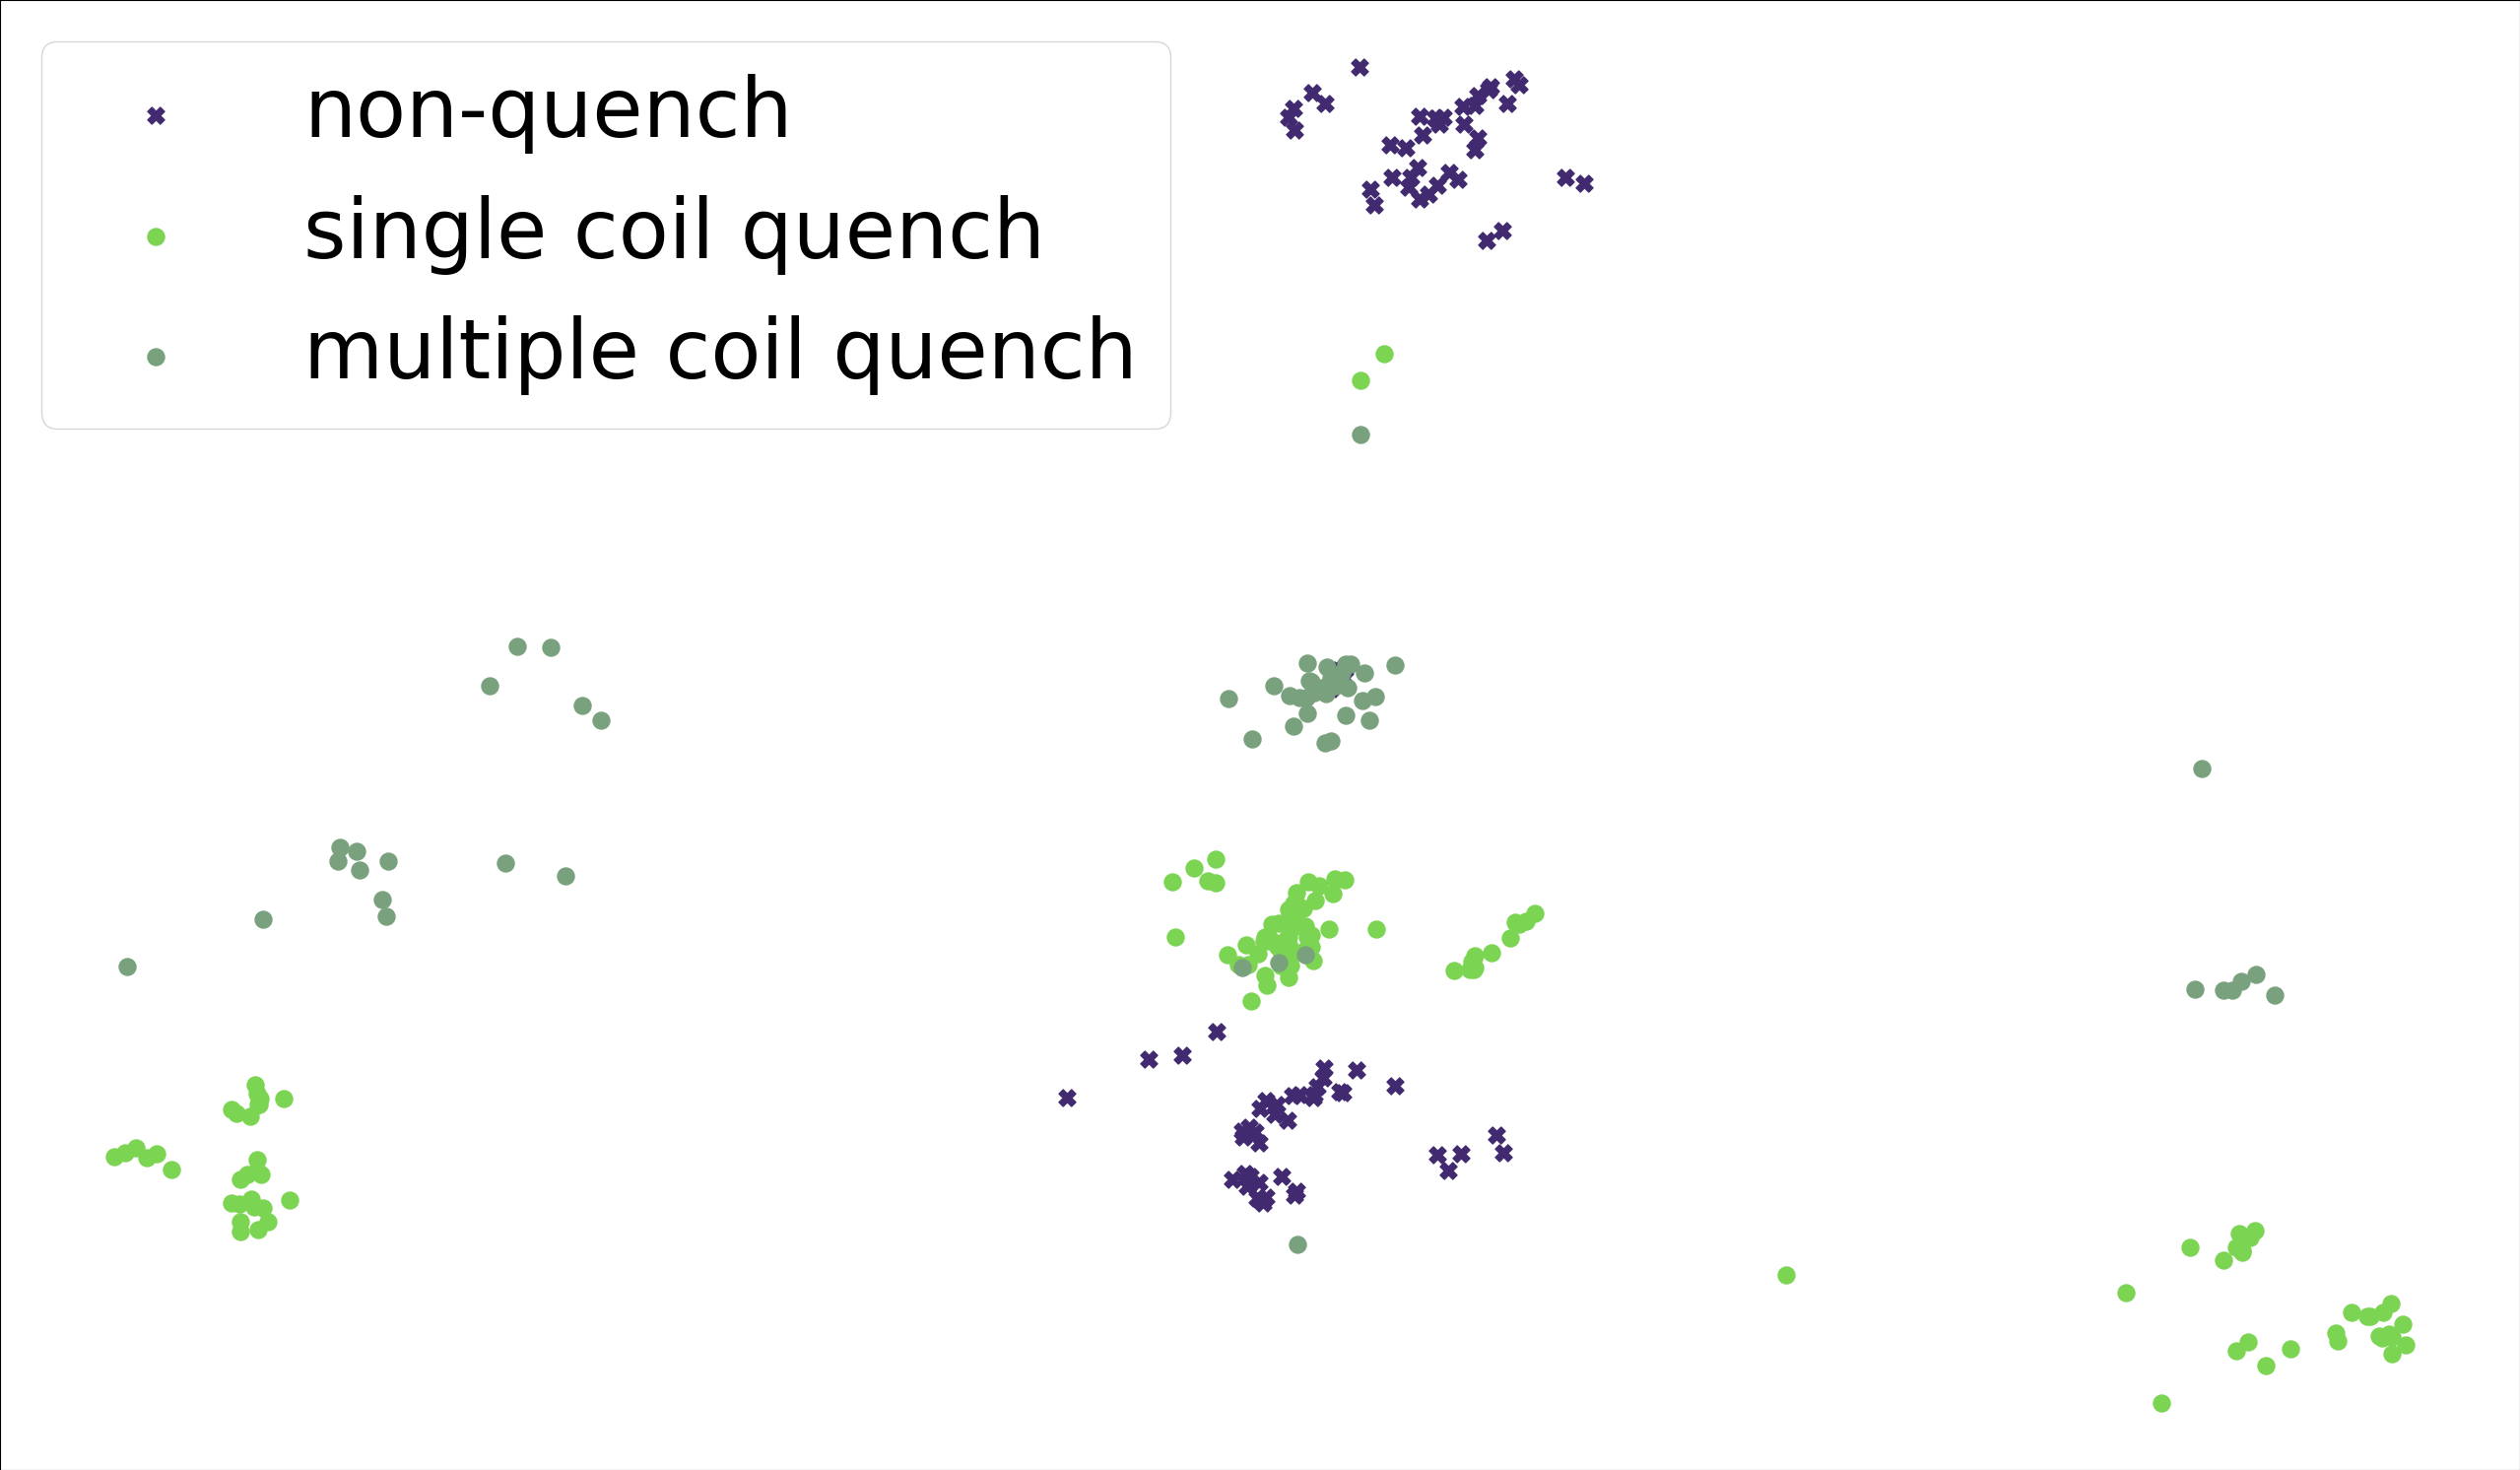
\includegraphics[width=\linewidth]{img/quench_dist_qlp/single_vs_multiple_An.png}
		\subcaption{}
	\end{subfigure}
	\begin{subfigure}{0.8\linewidth}
		\centering
		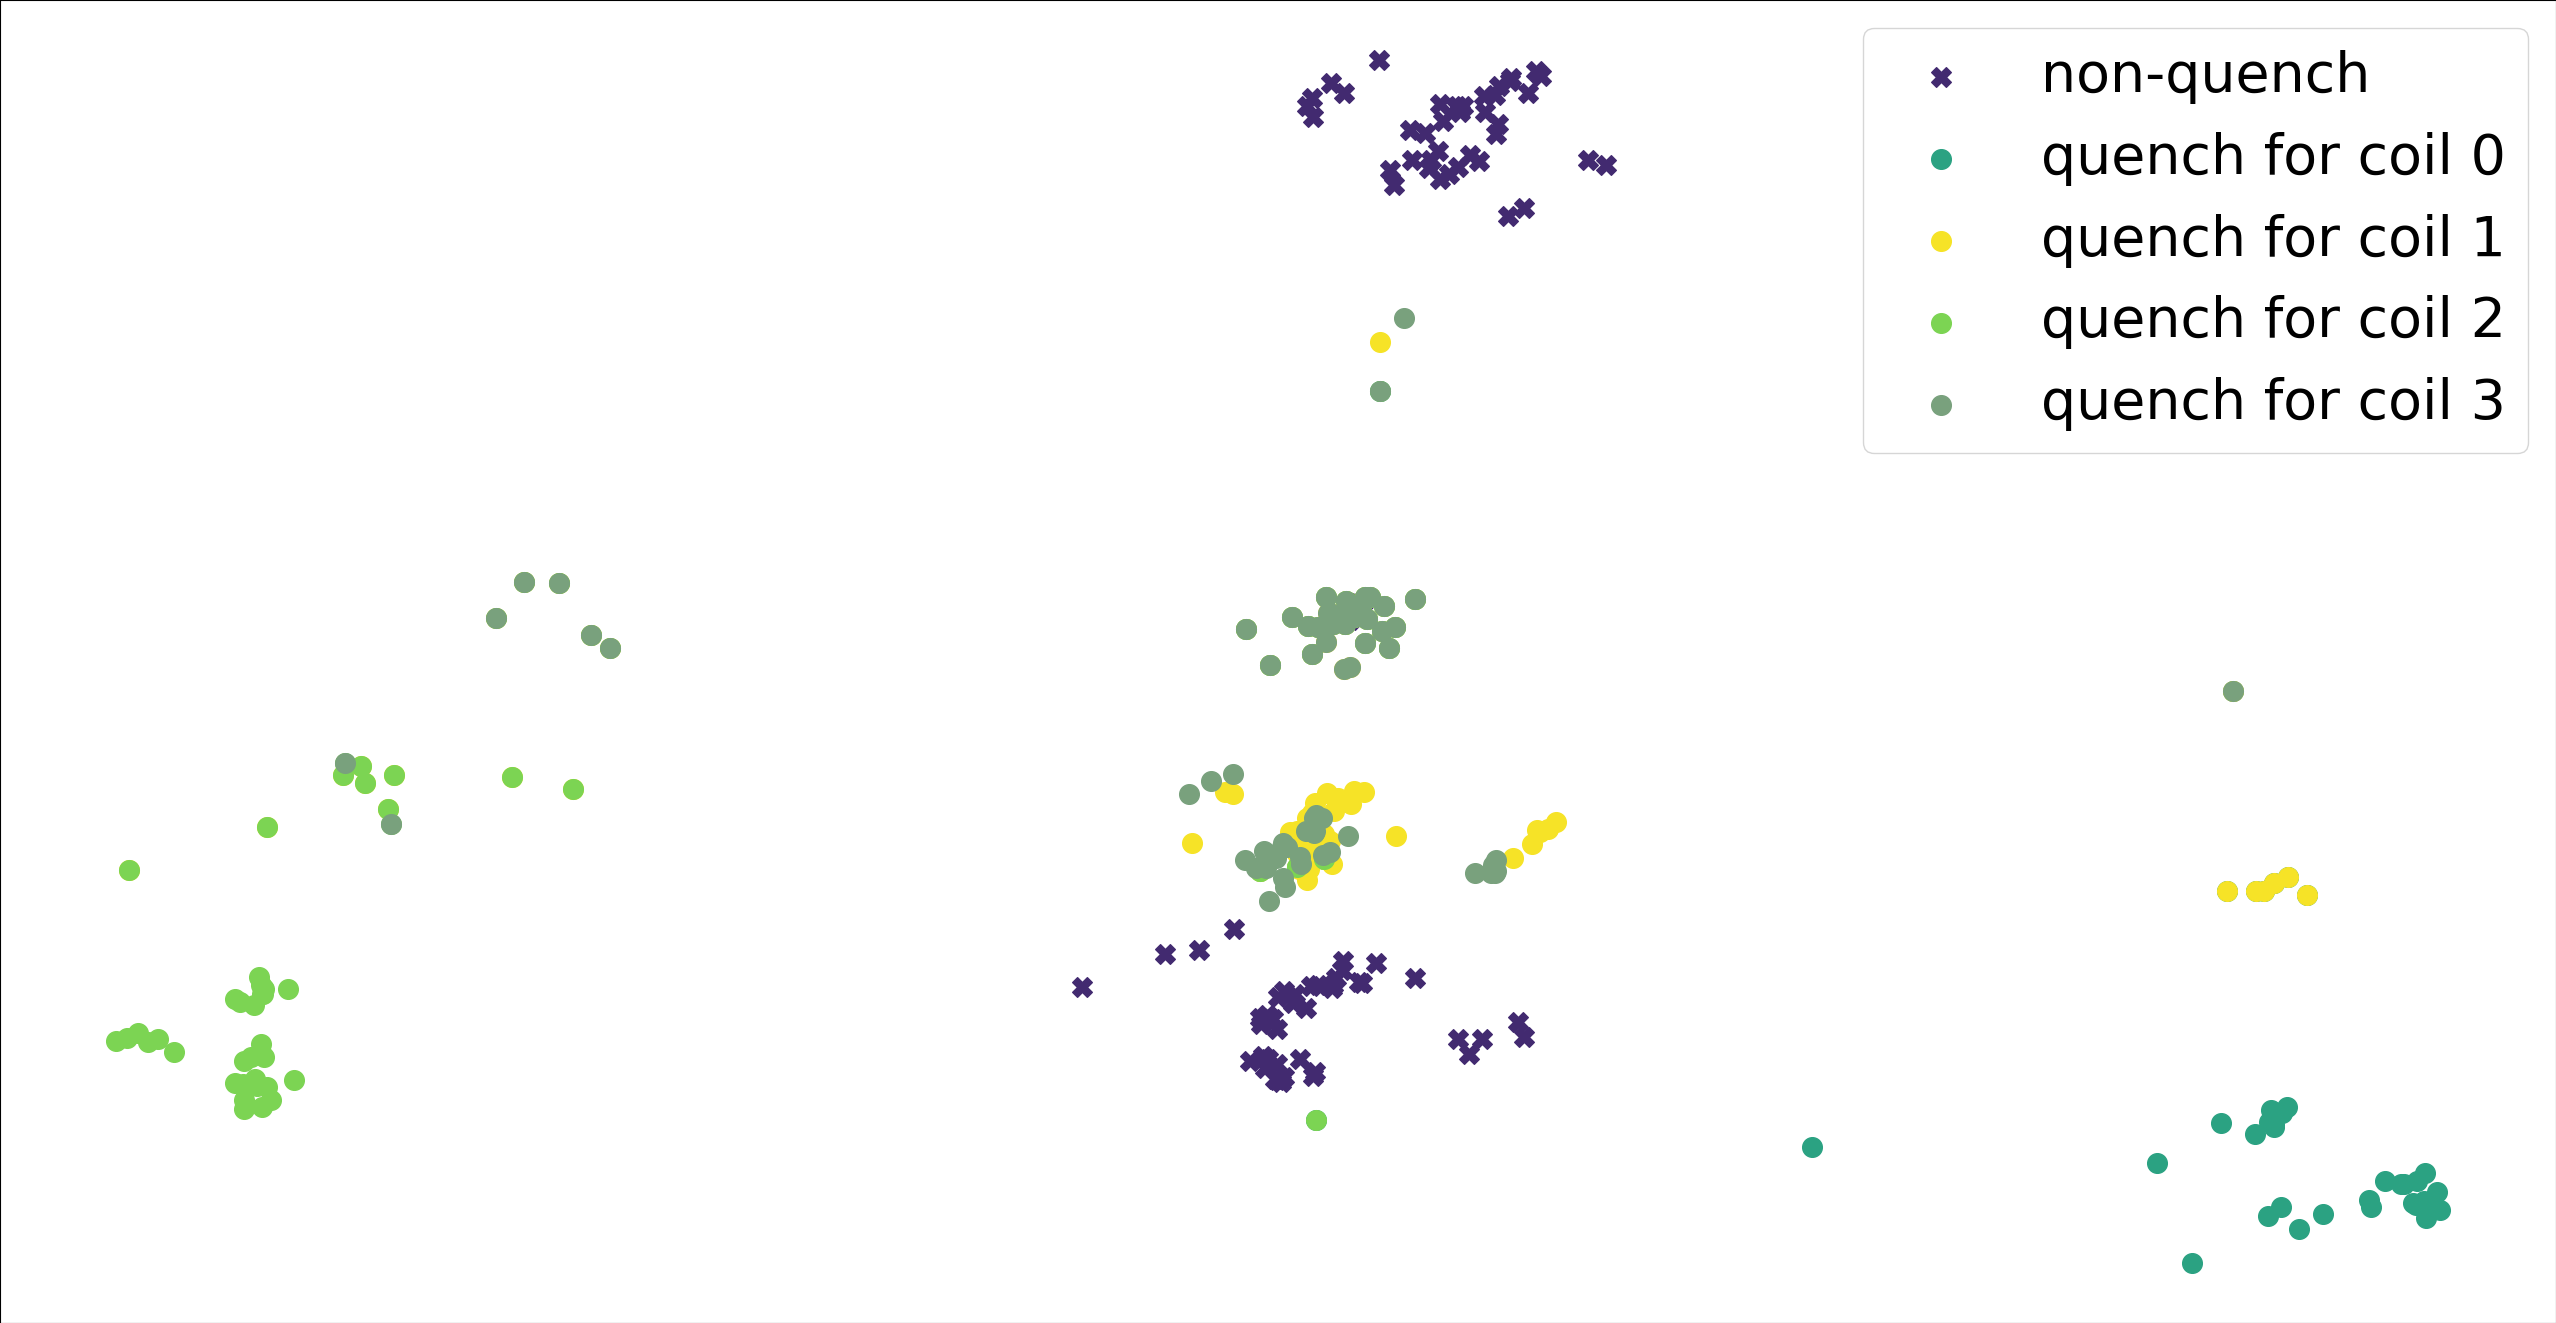
\includegraphics[width=\linewidth]{img/quench_dist_qlp_an.png}
		\subcaption{}
	\end{subfigure}
	\caption{Visualization of the \an\ attribute, the data was plotted after a run of \pca\
		dimensionality reduction. Sub-figure (a) highlights the samples based on how many quenches
		are associated to the specific sample $\{0, 1, \text{many}\}$. Sub-figure (b) highlights the
		samples based on the specific coil quenched $\{\text{None}, 0, 1, 2, 3\}$.}\label{fig:an-coilq-dist}
\end{figure}

\subsubsection{\bn}
While experimenting with \qrp, we discovered that \bn\ was the attribute that performed the least
among the ones available. We expected similar results for \qlp, but from preprocessing alone we
could not understand whether the attribute promised good or bad performance.

\Cref{fig:bn-lcorr-qlp} highlights the correlation between \bn\ harmonics and the label associated
to each coil (as described in \Cref{chp:problem}). The attribute, similarly to \an, sees a pattern
of strong correlations between its odd-numbered harmonics and coils $1$ and $3$. Since the pattern
of sub-figures (b) and (d) is very similar to the one shown in sub-figures (a) and (c) of
\Cref{fig:an-lcorr-qlp}, we imagined that a plausible dataset composition would have followed rules
similar to the ones identified for \an.
\begin{figure}[!ht]
	% Font size = 70
	\centering
	\begin{subfigure}{0.49\linewidth}
		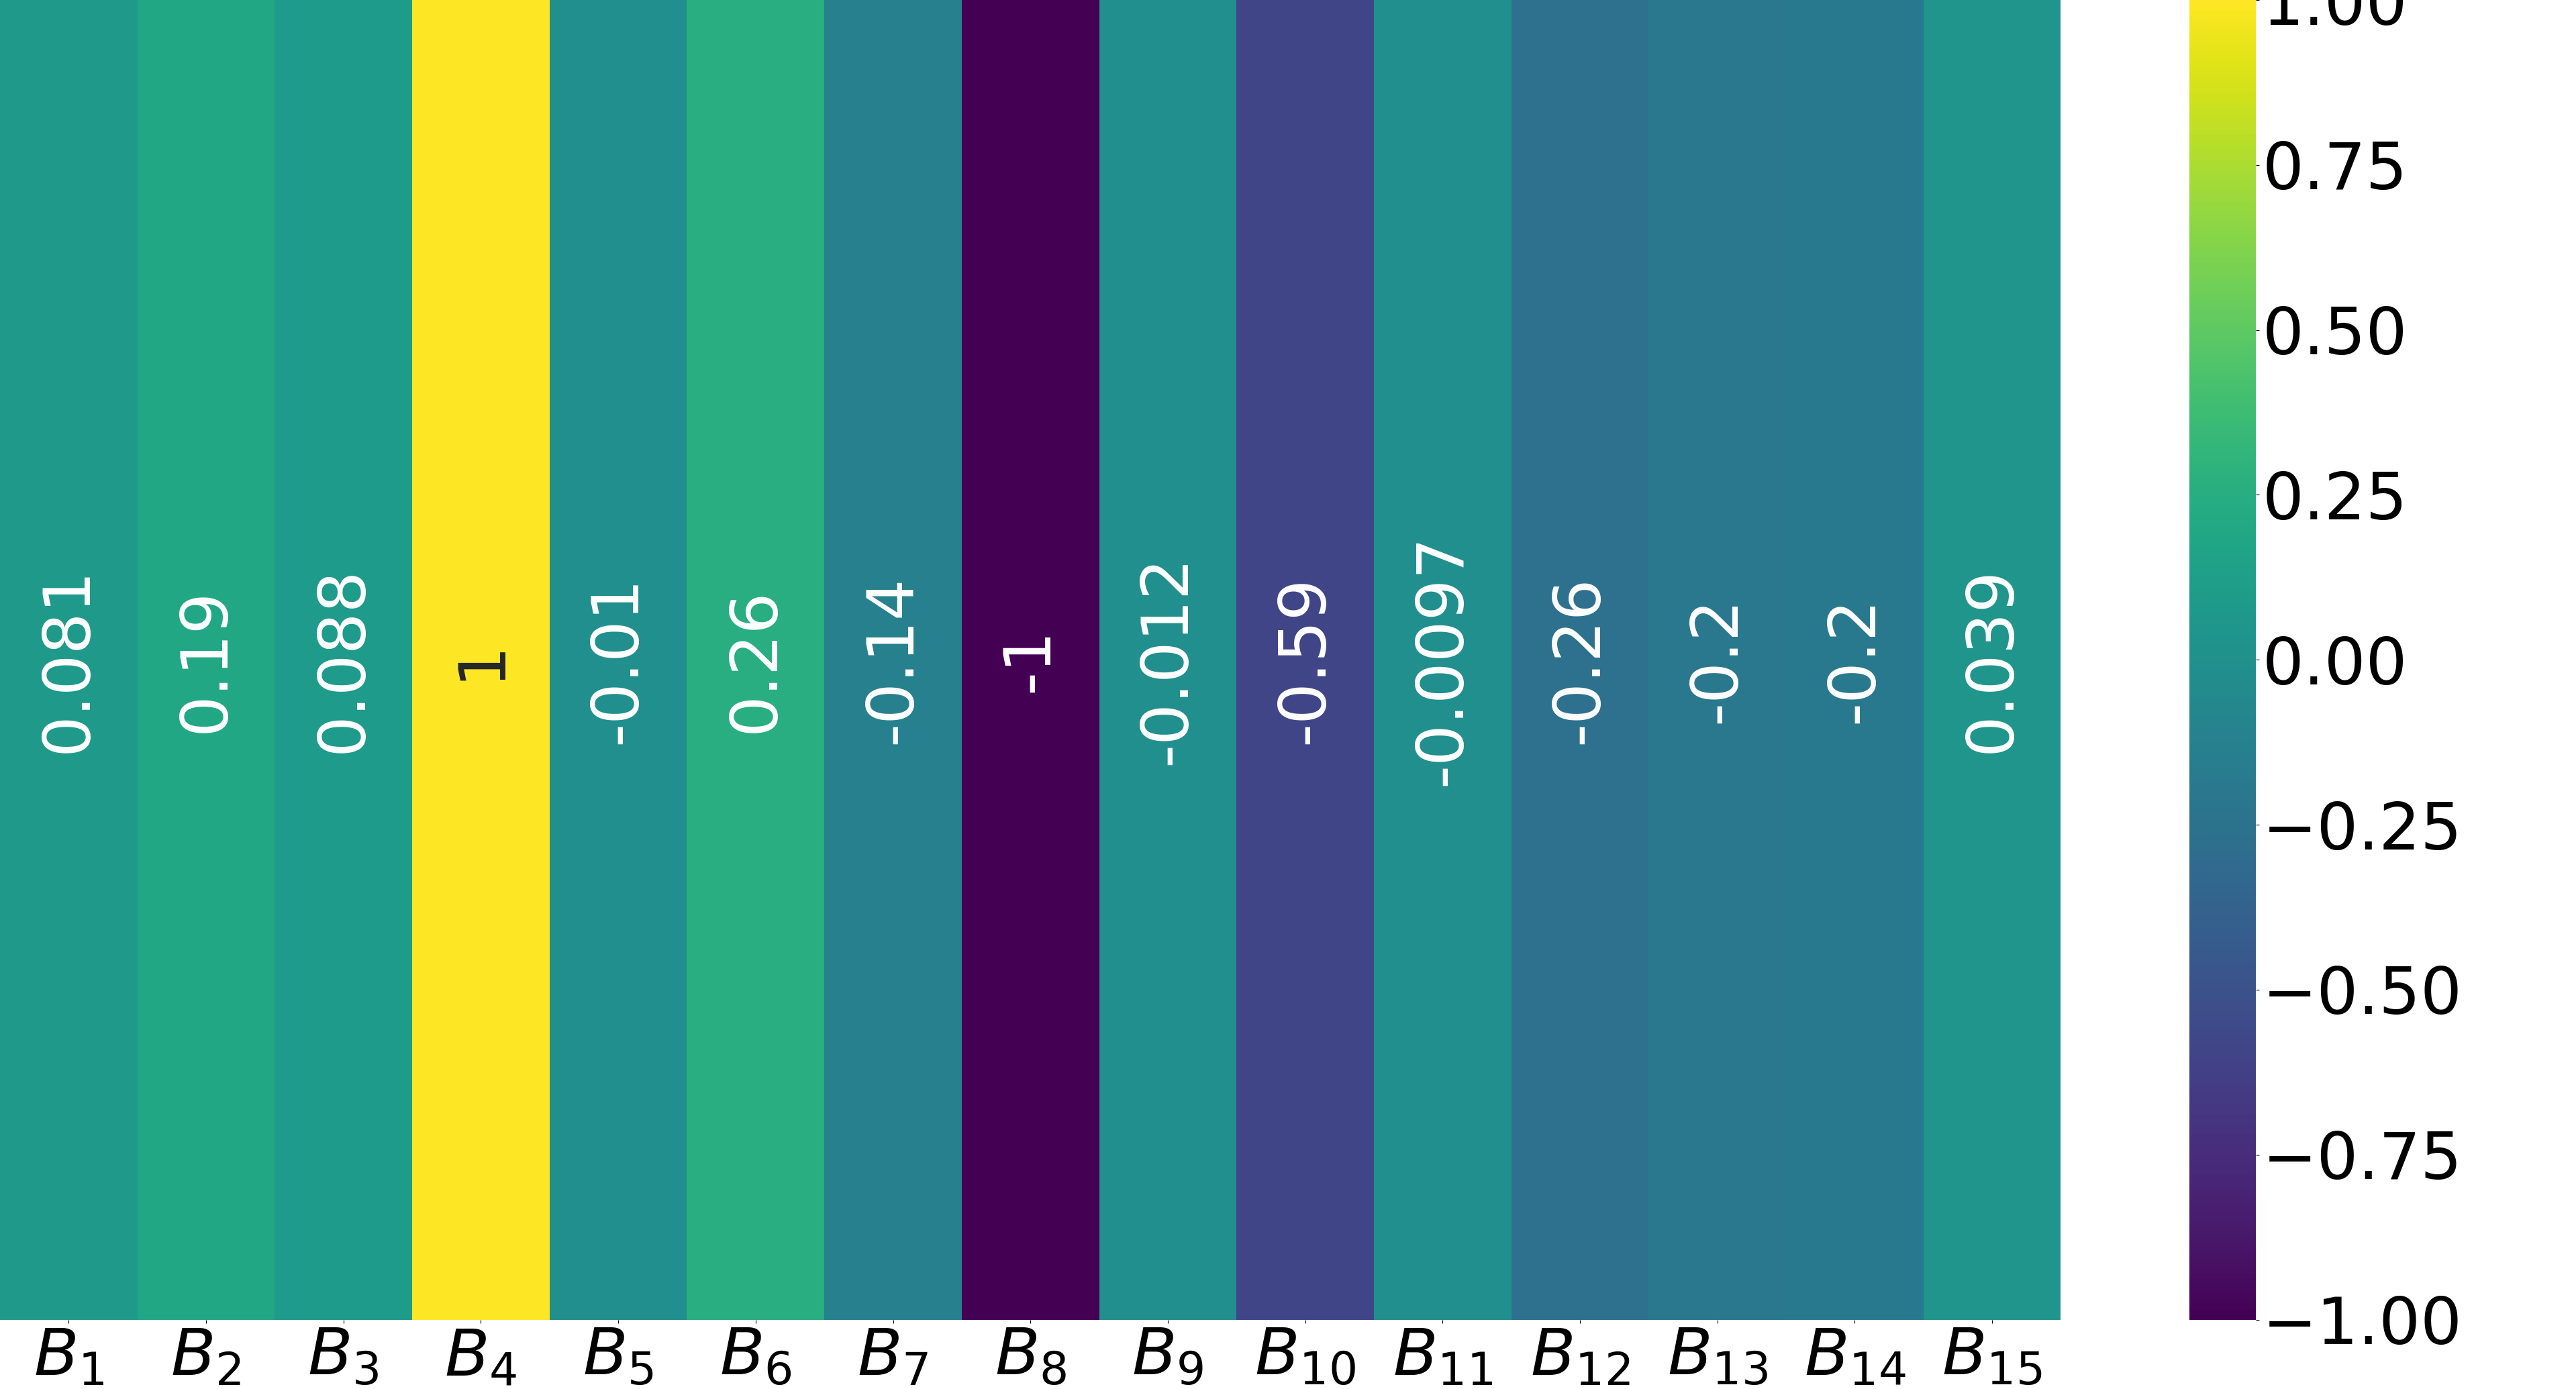
\includegraphics[width=\linewidth]{img/qlp_corr/Bn_coil0.png}
		\subcaption{Correlation with coil $0$}
	\end{subfigure}
	\begin{subfigure}{0.49\linewidth}
		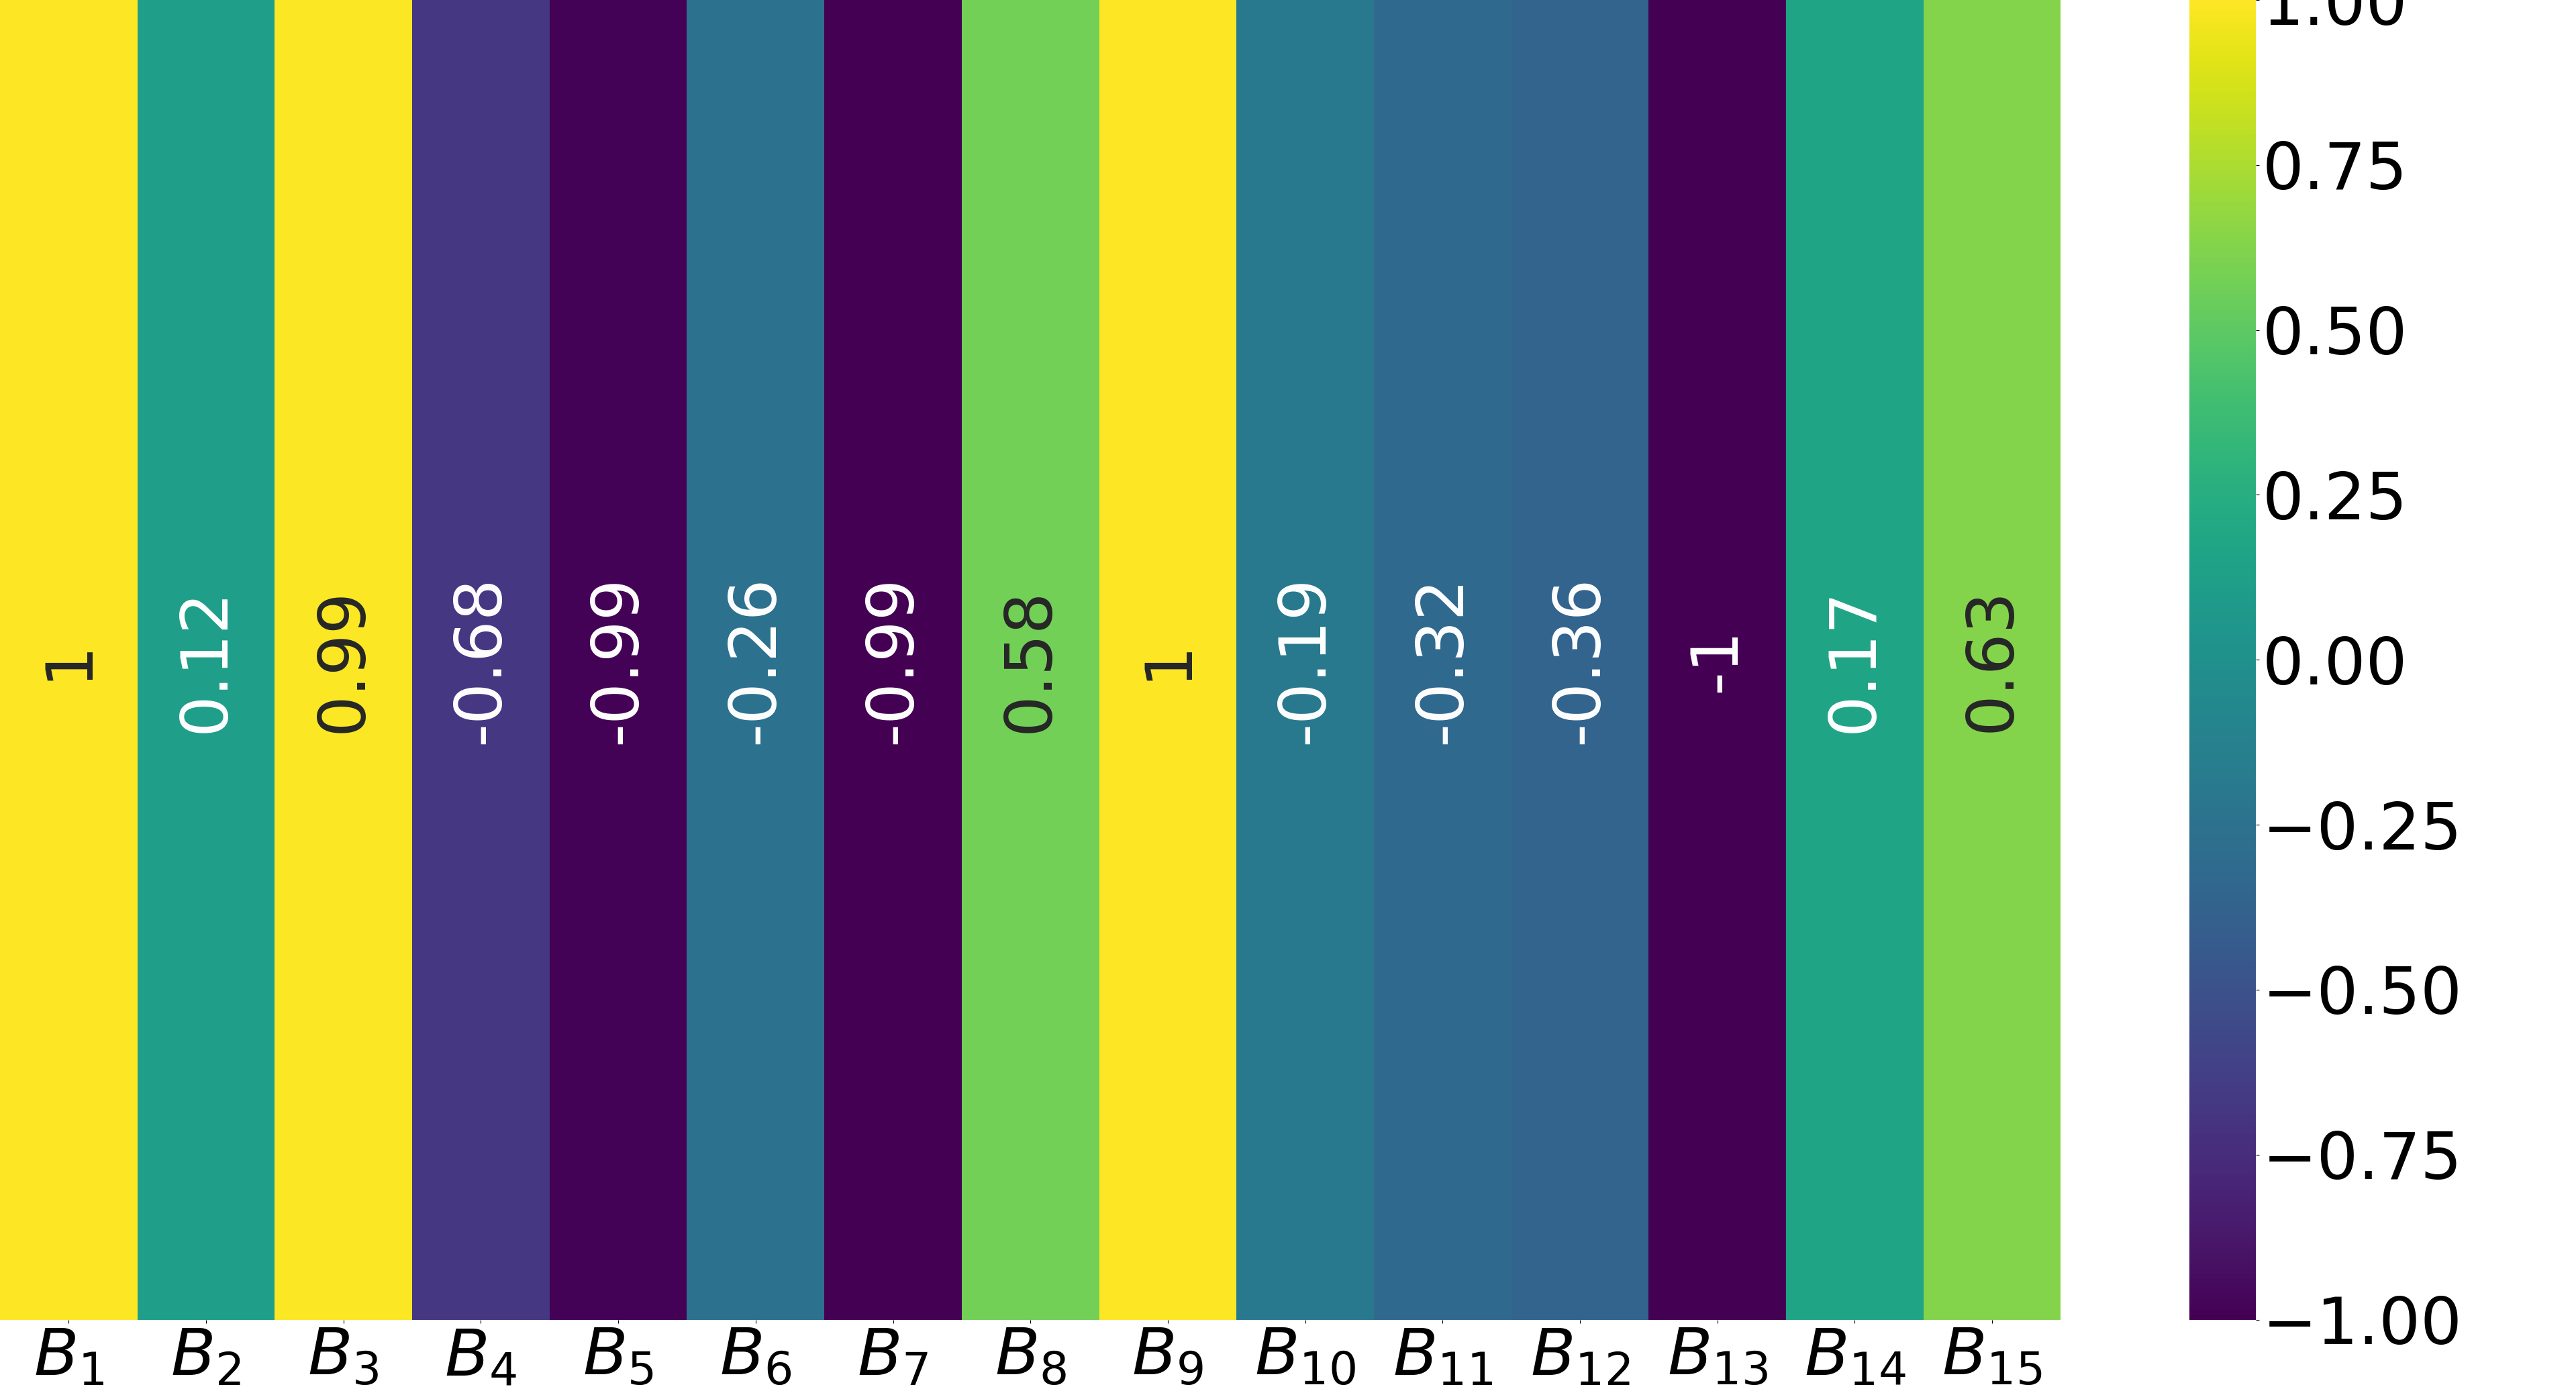
\includegraphics[width=\linewidth]{img/qlp_corr/Bn_coil1.png}
		\subcaption{Correlation with coil $1$}
	\end{subfigure}
	\begin{subfigure}{0.49\linewidth}
		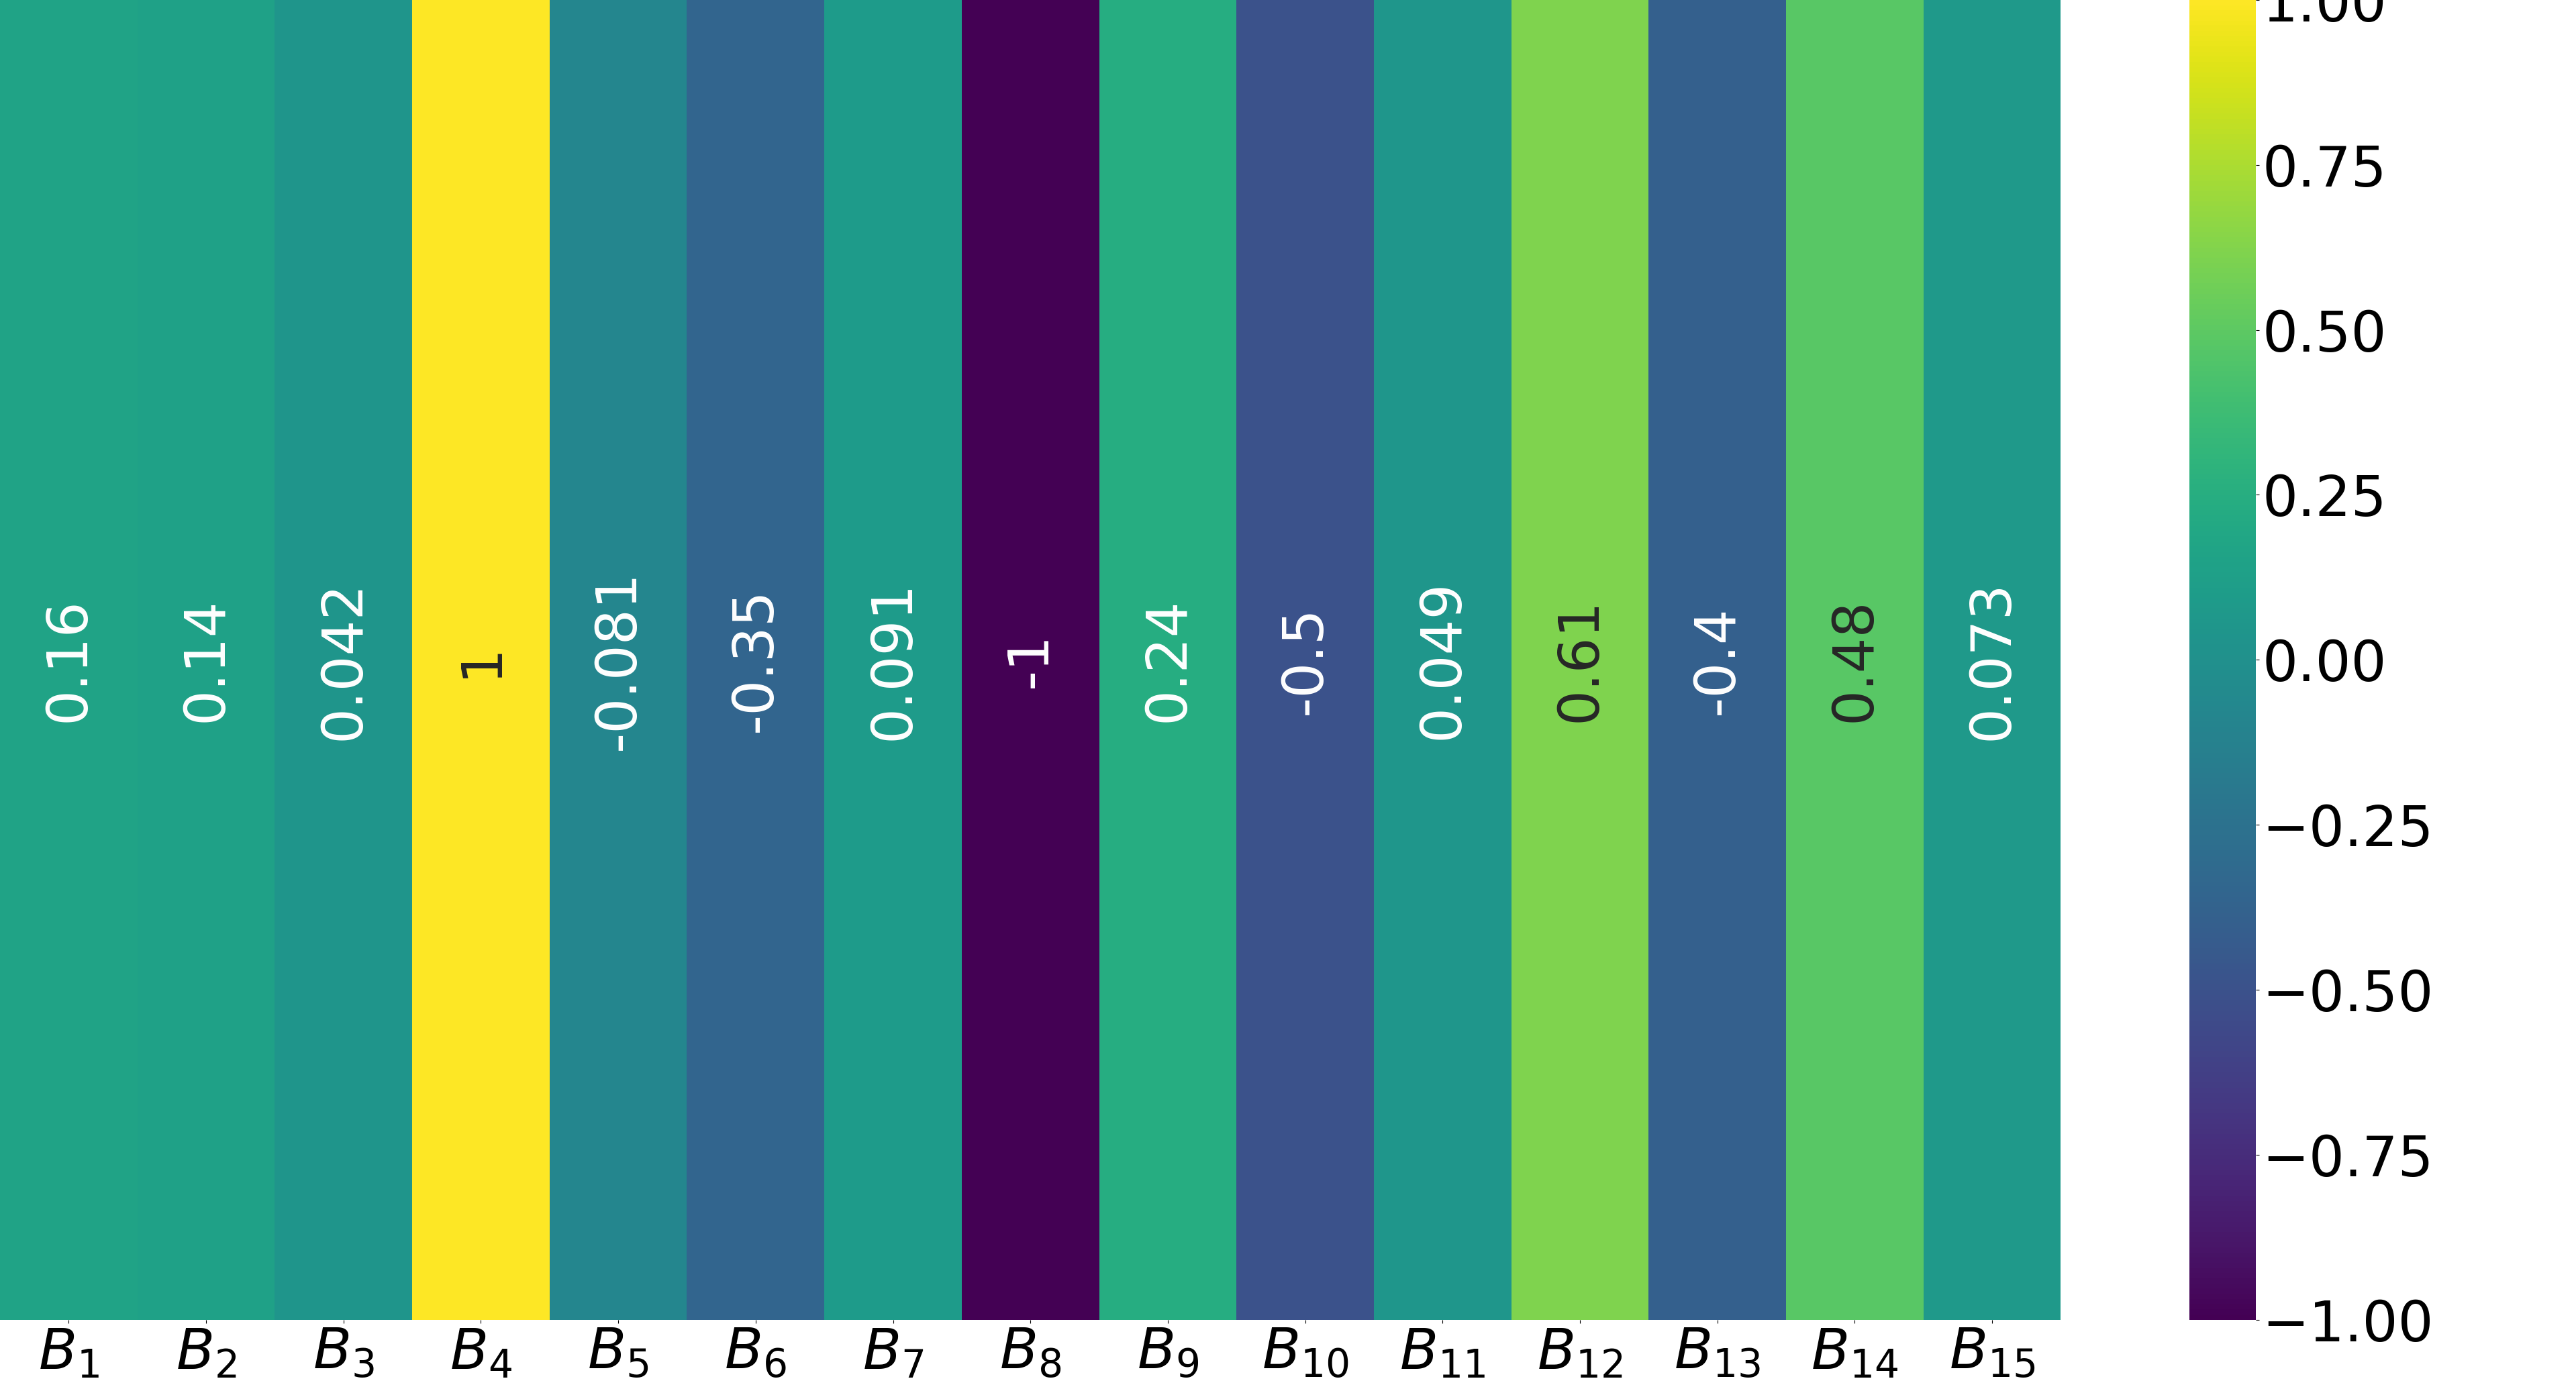
\includegraphics[width=\linewidth]{img/qlp_corr/Bn_coil2.png}
		\subcaption{Correlation with coil $2$}
	\end{subfigure}
	\begin{subfigure}{0.49\linewidth}
		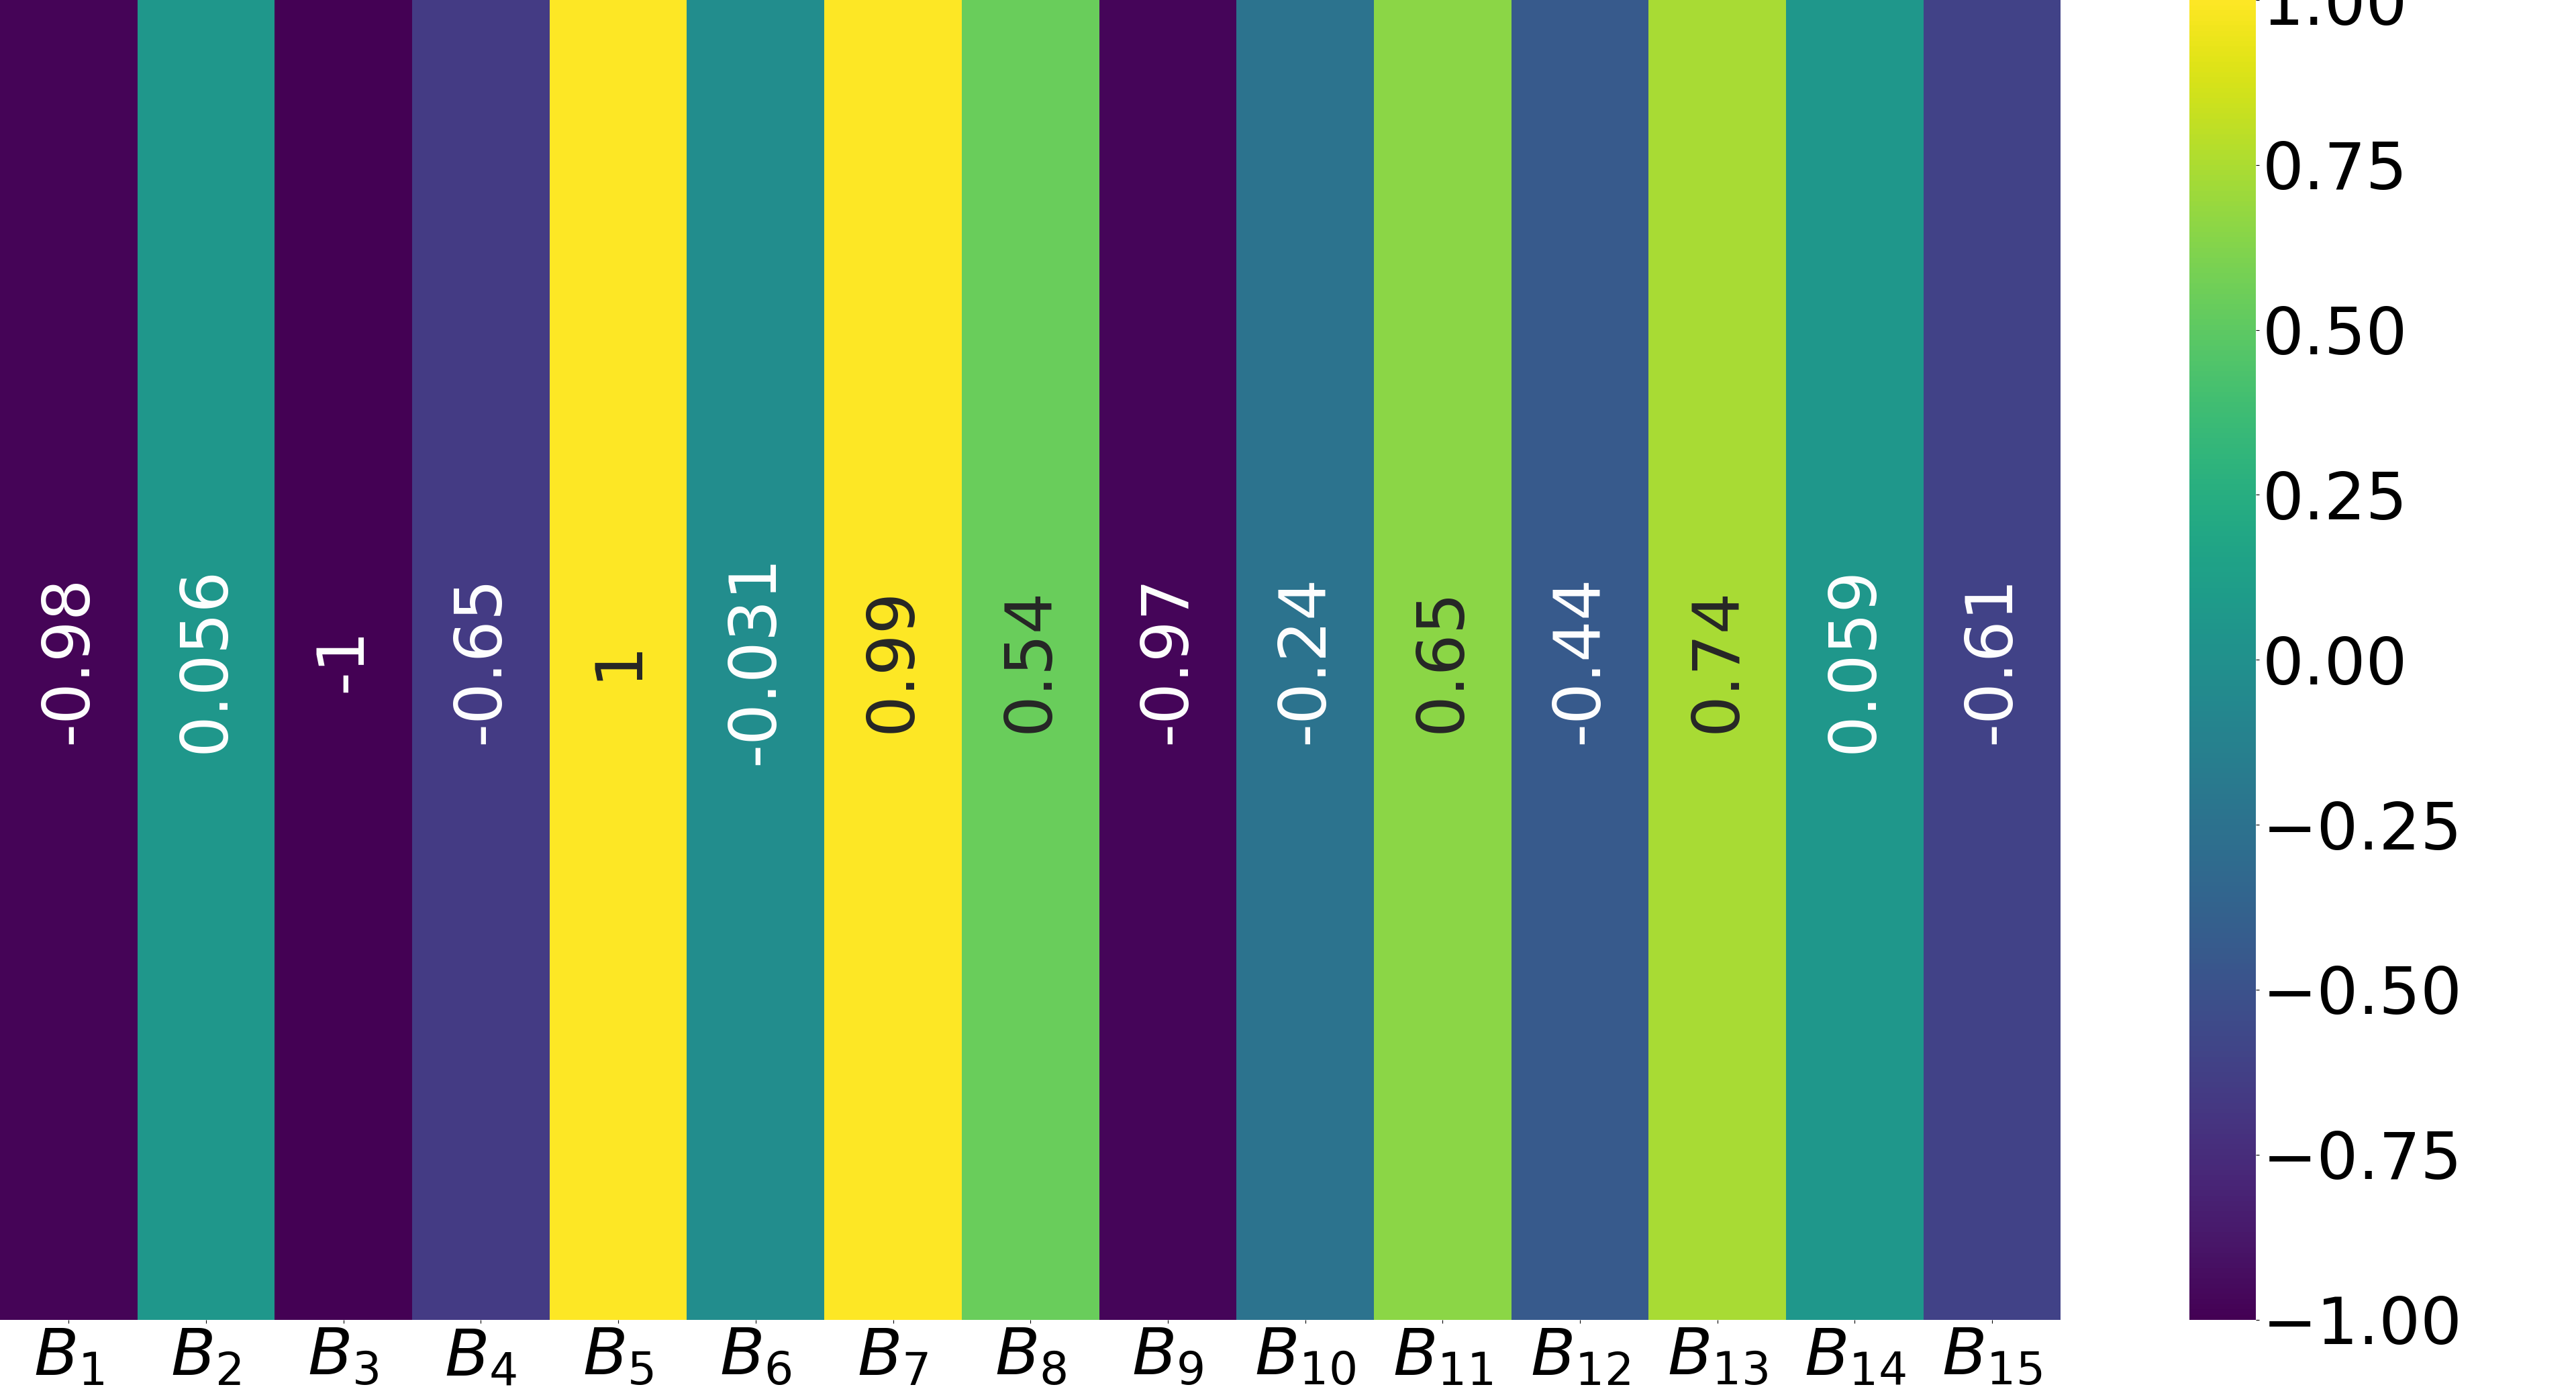
\includegraphics[width=\linewidth]{img/qlp_corr/Bn_coil3.png}
		\subcaption{Correlation with coil $3$}
	\end{subfigure}
	\caption{Correlation between the harmonics of the \bn\ attribute and the labels for \qlp.}
	\label{fig:bn-lcorr-qlp}
\end{figure}

In \Cref{fig:bn-coilq-dist} we visualized the samples in \bn\ after a round of \pca. Independently of the sub-figure we consider it's clear that the level of
homogeneity of the samples belonging to the central cluster is very high. While this, alone, cannot
induce us to think that the performance of models based on \bn\ is going to be bad, we are drawn to
consider the possibility that \bn\ might not be a good enough attribute if taken on its own.
\begin{figure}[!ht]
	% Font size = 40
	\centering
	\begin{subfigure}{0.8\linewidth}
		\centering
		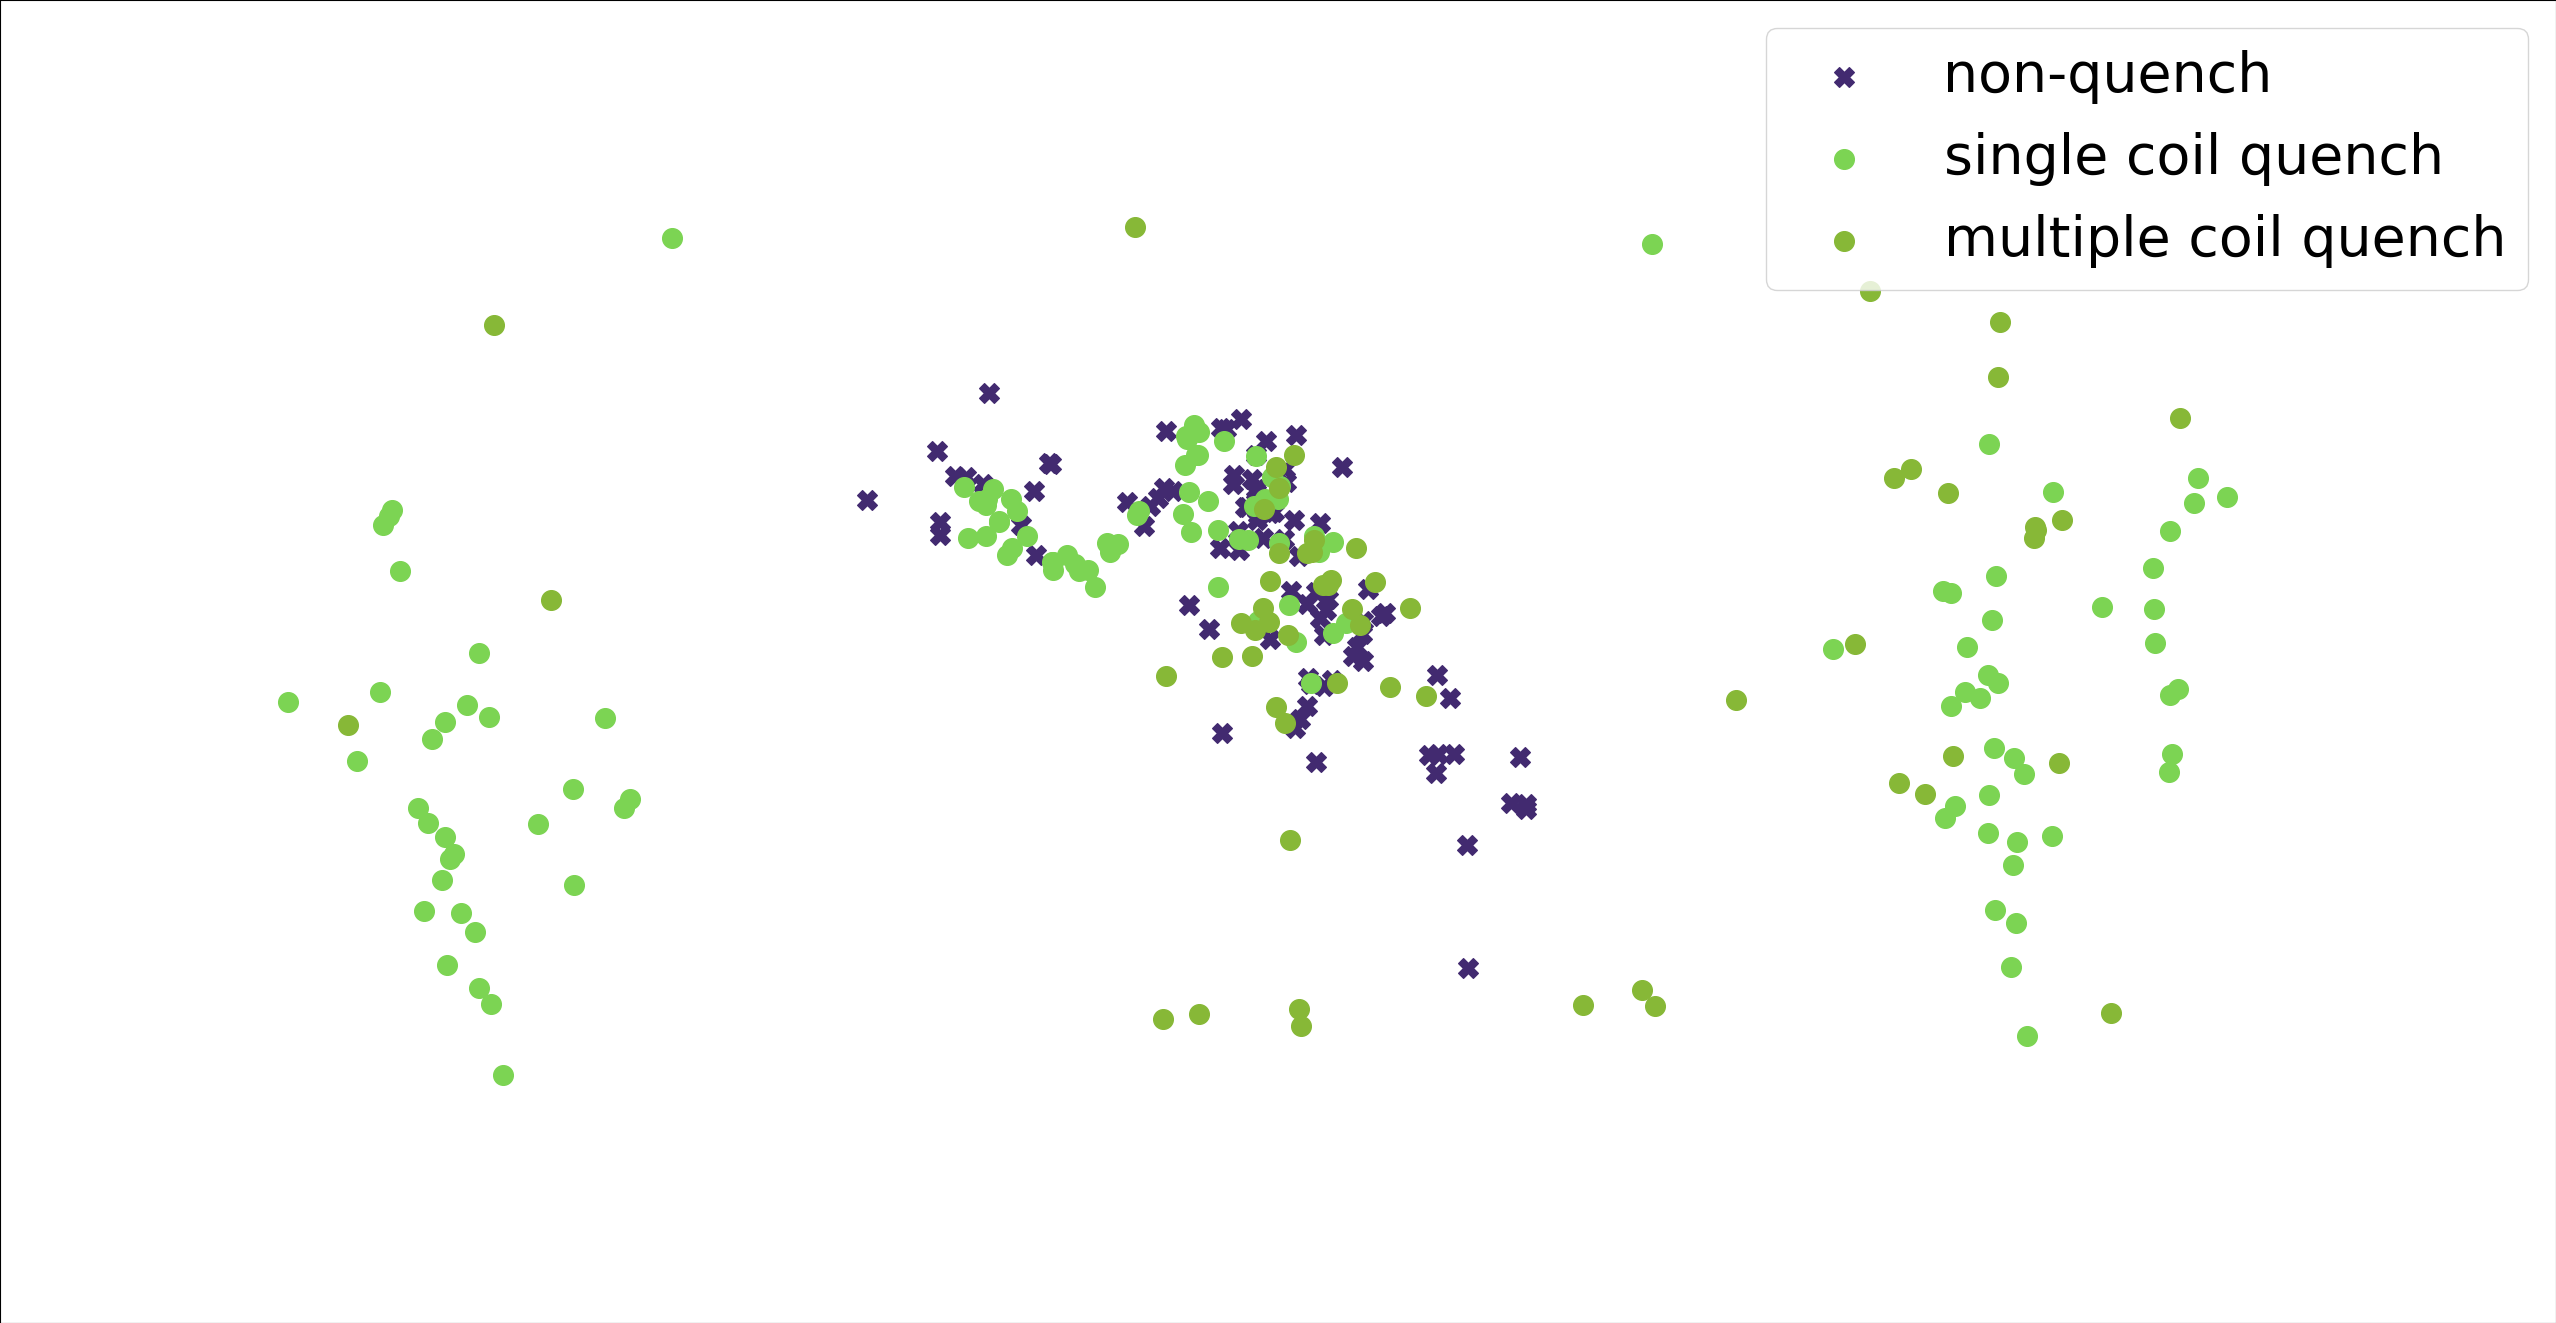
\includegraphics[width=\linewidth]{img/quench_dist_qlp/single_vs_multiple_Bn.png}
		\subcaption{}
	\end{subfigure}
	\begin{subfigure}{0.8\linewidth}
		\centering
		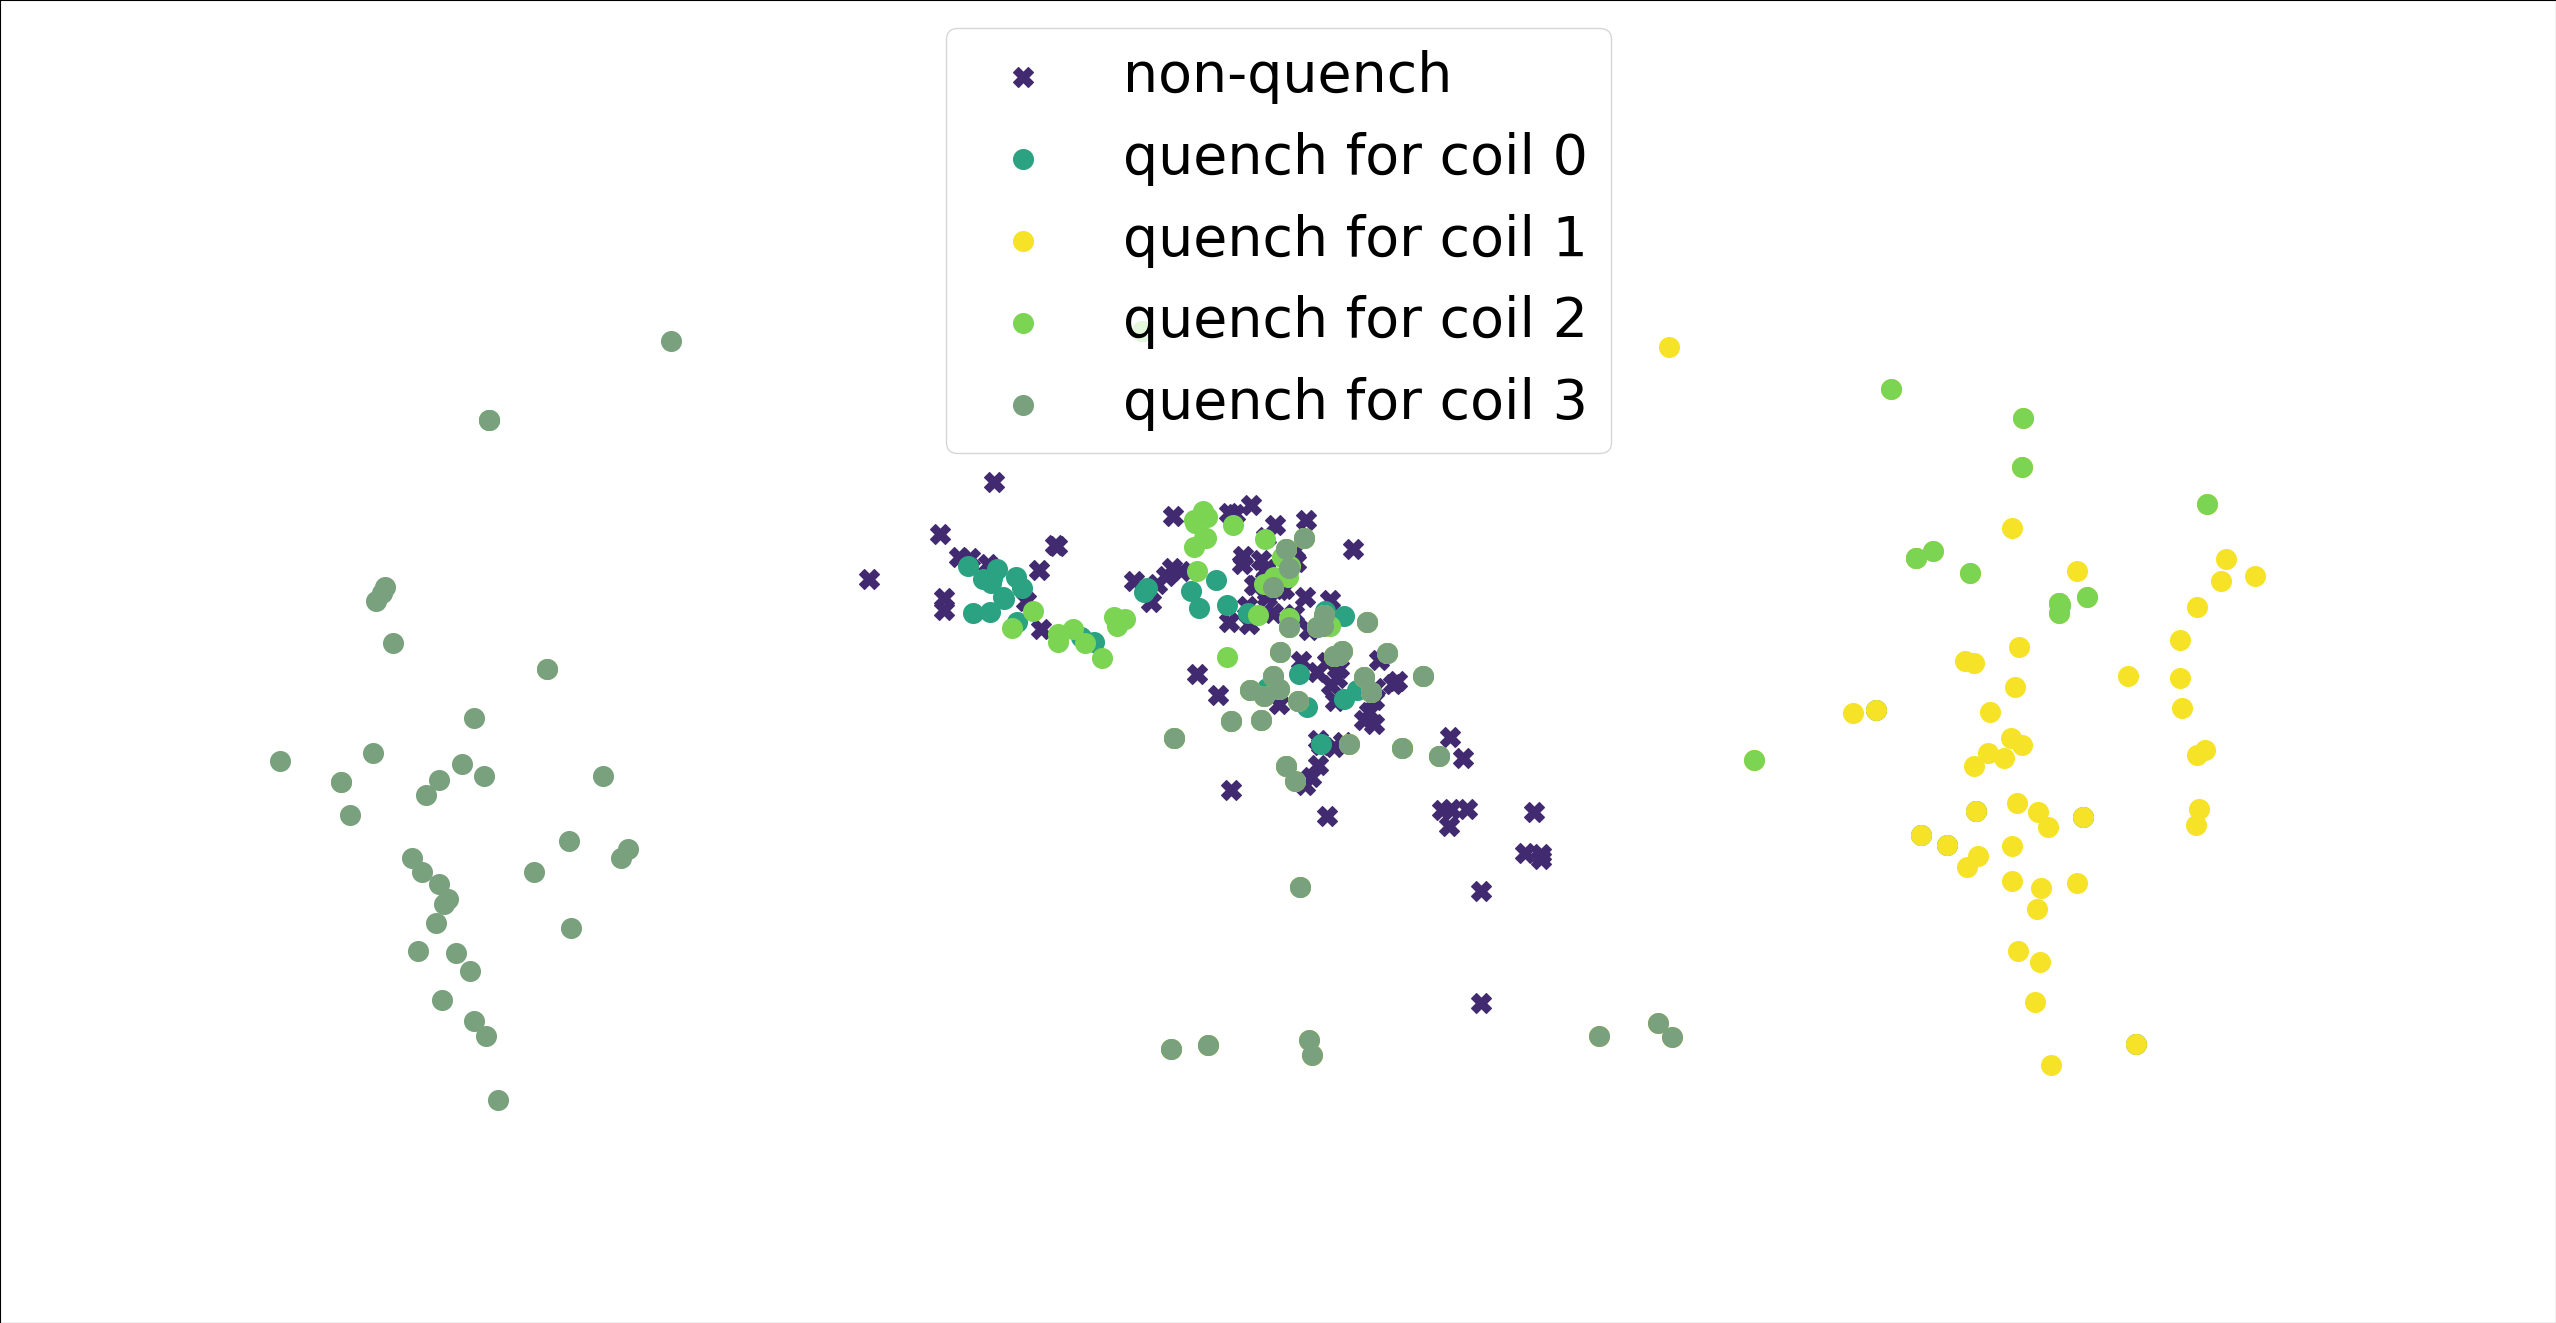
\includegraphics[width=\linewidth]{img/quench_dist_qlp_bn.png}
		\subcaption{}
	\end{subfigure}
	\caption{Visualization of the \bn\ attribute, the data was plotted after a run of \pca\
		dimensionality reduction. Sub-figure (a) highlights the samples based on how many quenches
		are associated to the specific sample $\{0, 1, \text{many}\}$. Sub-figure (b) highlights the
		samples based on the specific coil quenched $\{\text{None}, 0, 1, 2, 3\}$.}
	\label{fig:bn-coilq-dist}
\end{figure}

\subsubsection{\cnmod}
As we said in \Cref{chp:problem}, \cnmod\ was expected to be very informative for \qrp, but not for
\qlp. Interestingly, though, the correlation between the harmonics for the attribute and the labels
associated to each coil, shown in \Cref{fig:cnmod-lcorr-qlp}, seem to be telling a different story.
If we consider coils $0$ and $3$, we can see a very strong correlation between the harmonics and the
label, it's also worth noting that, in sub-figures (a) through (d), \cnmod[2]\ seems to be extremely
important to explain the value associated with the labels.

If we look back at the correlation matrix computed for \cnmod\ during the preprocessing for \qrp\
(cfr. \Cref{fig:cnmod-corr}) a sub-view of \cnmod\ could be built as follows:
\begin{itemize}
	\item For coil $0$, \cnmod[2] and adding a high-order candidate. While this would technically maximize the total correlation with the label, we have seen in \qrp\ that choosing \cnmod[2]\ was a choice that didn't pay. That is why we might select \cnmod[3] or \cnmod[6] in the end, accompanied by another high order harmonic like \cnmod[9] or \cnmod[11].
	\item For coil $3$, we could be taking harmonic \cnmod[1] and then using one or more from
	      \{\cnmod[4], \cnmod[5], \cnmod[6], \cnmod[7], \cnmod[8]\}; finally, if it leads to
	      better performance, we could also add another high-order harmonic like \cnmod[10].
\end{itemize}
\begin{figure}[!ht]
	% Font size = 70
	\centering
	\begin{subfigure}{0.49\linewidth}
		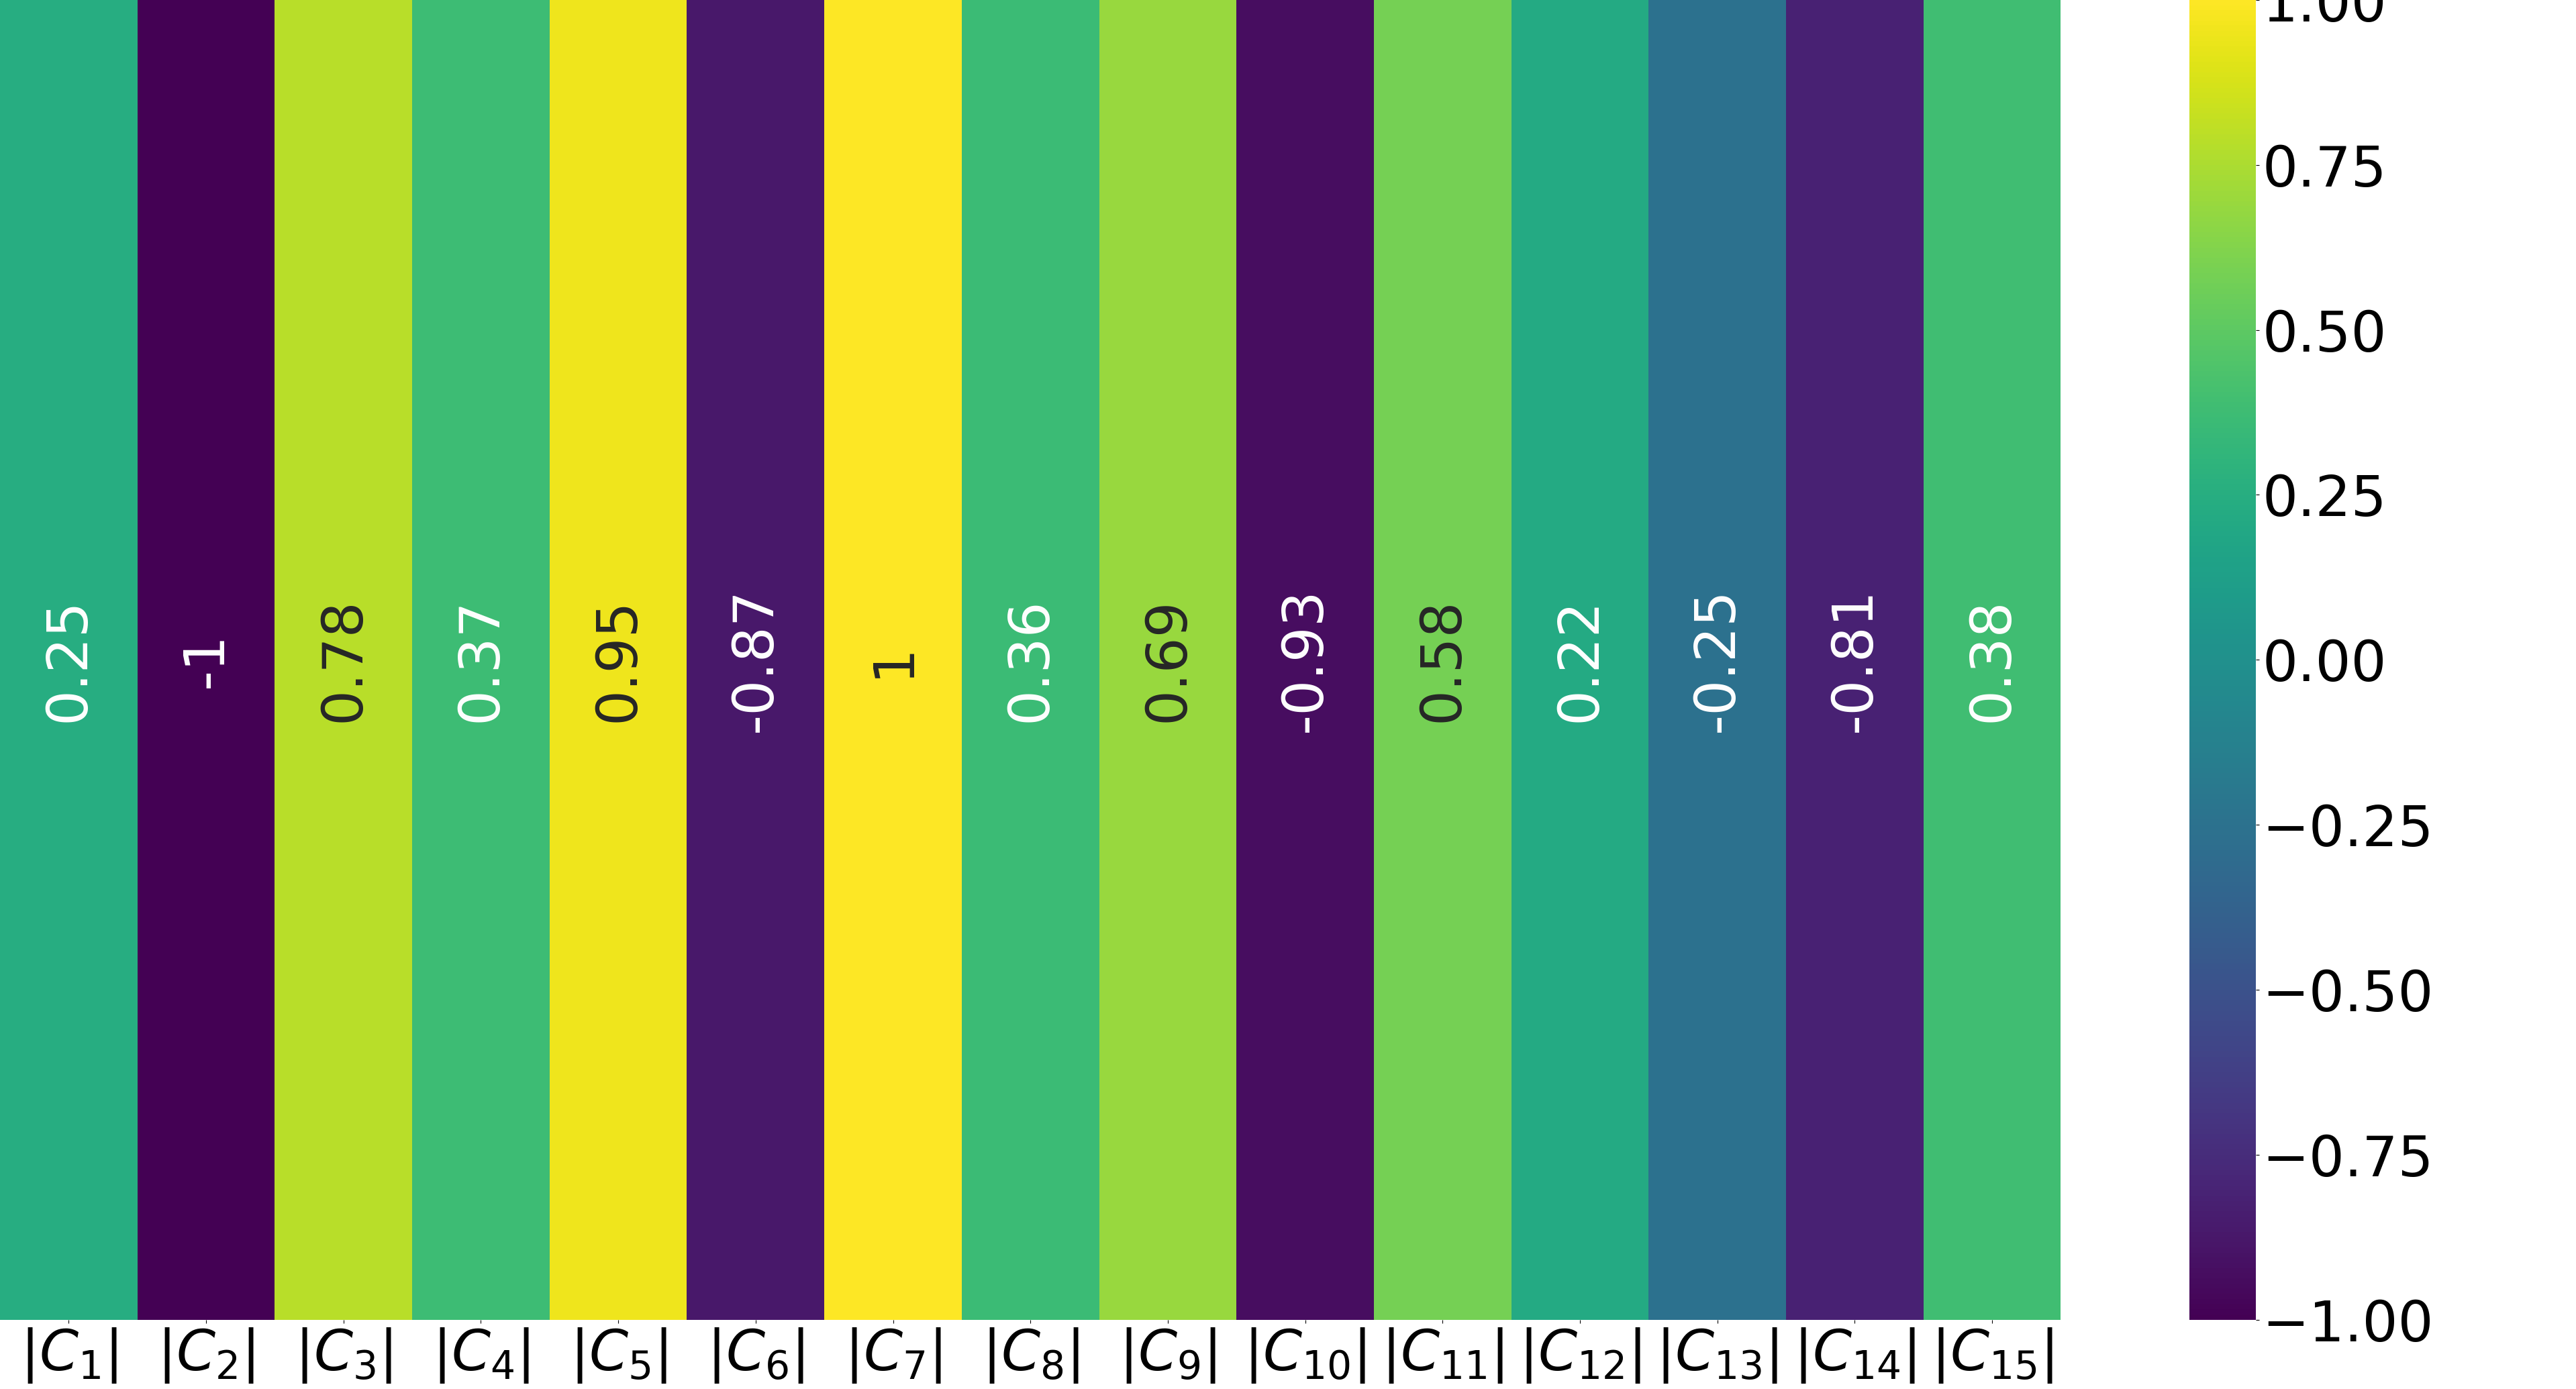
\includegraphics[width=\linewidth]{img/qlp_corr/Cnmod_coil0.png}
		\subcaption{Correlation with coil $0$}
	\end{subfigure}
	\begin{subfigure}{0.49\linewidth}
		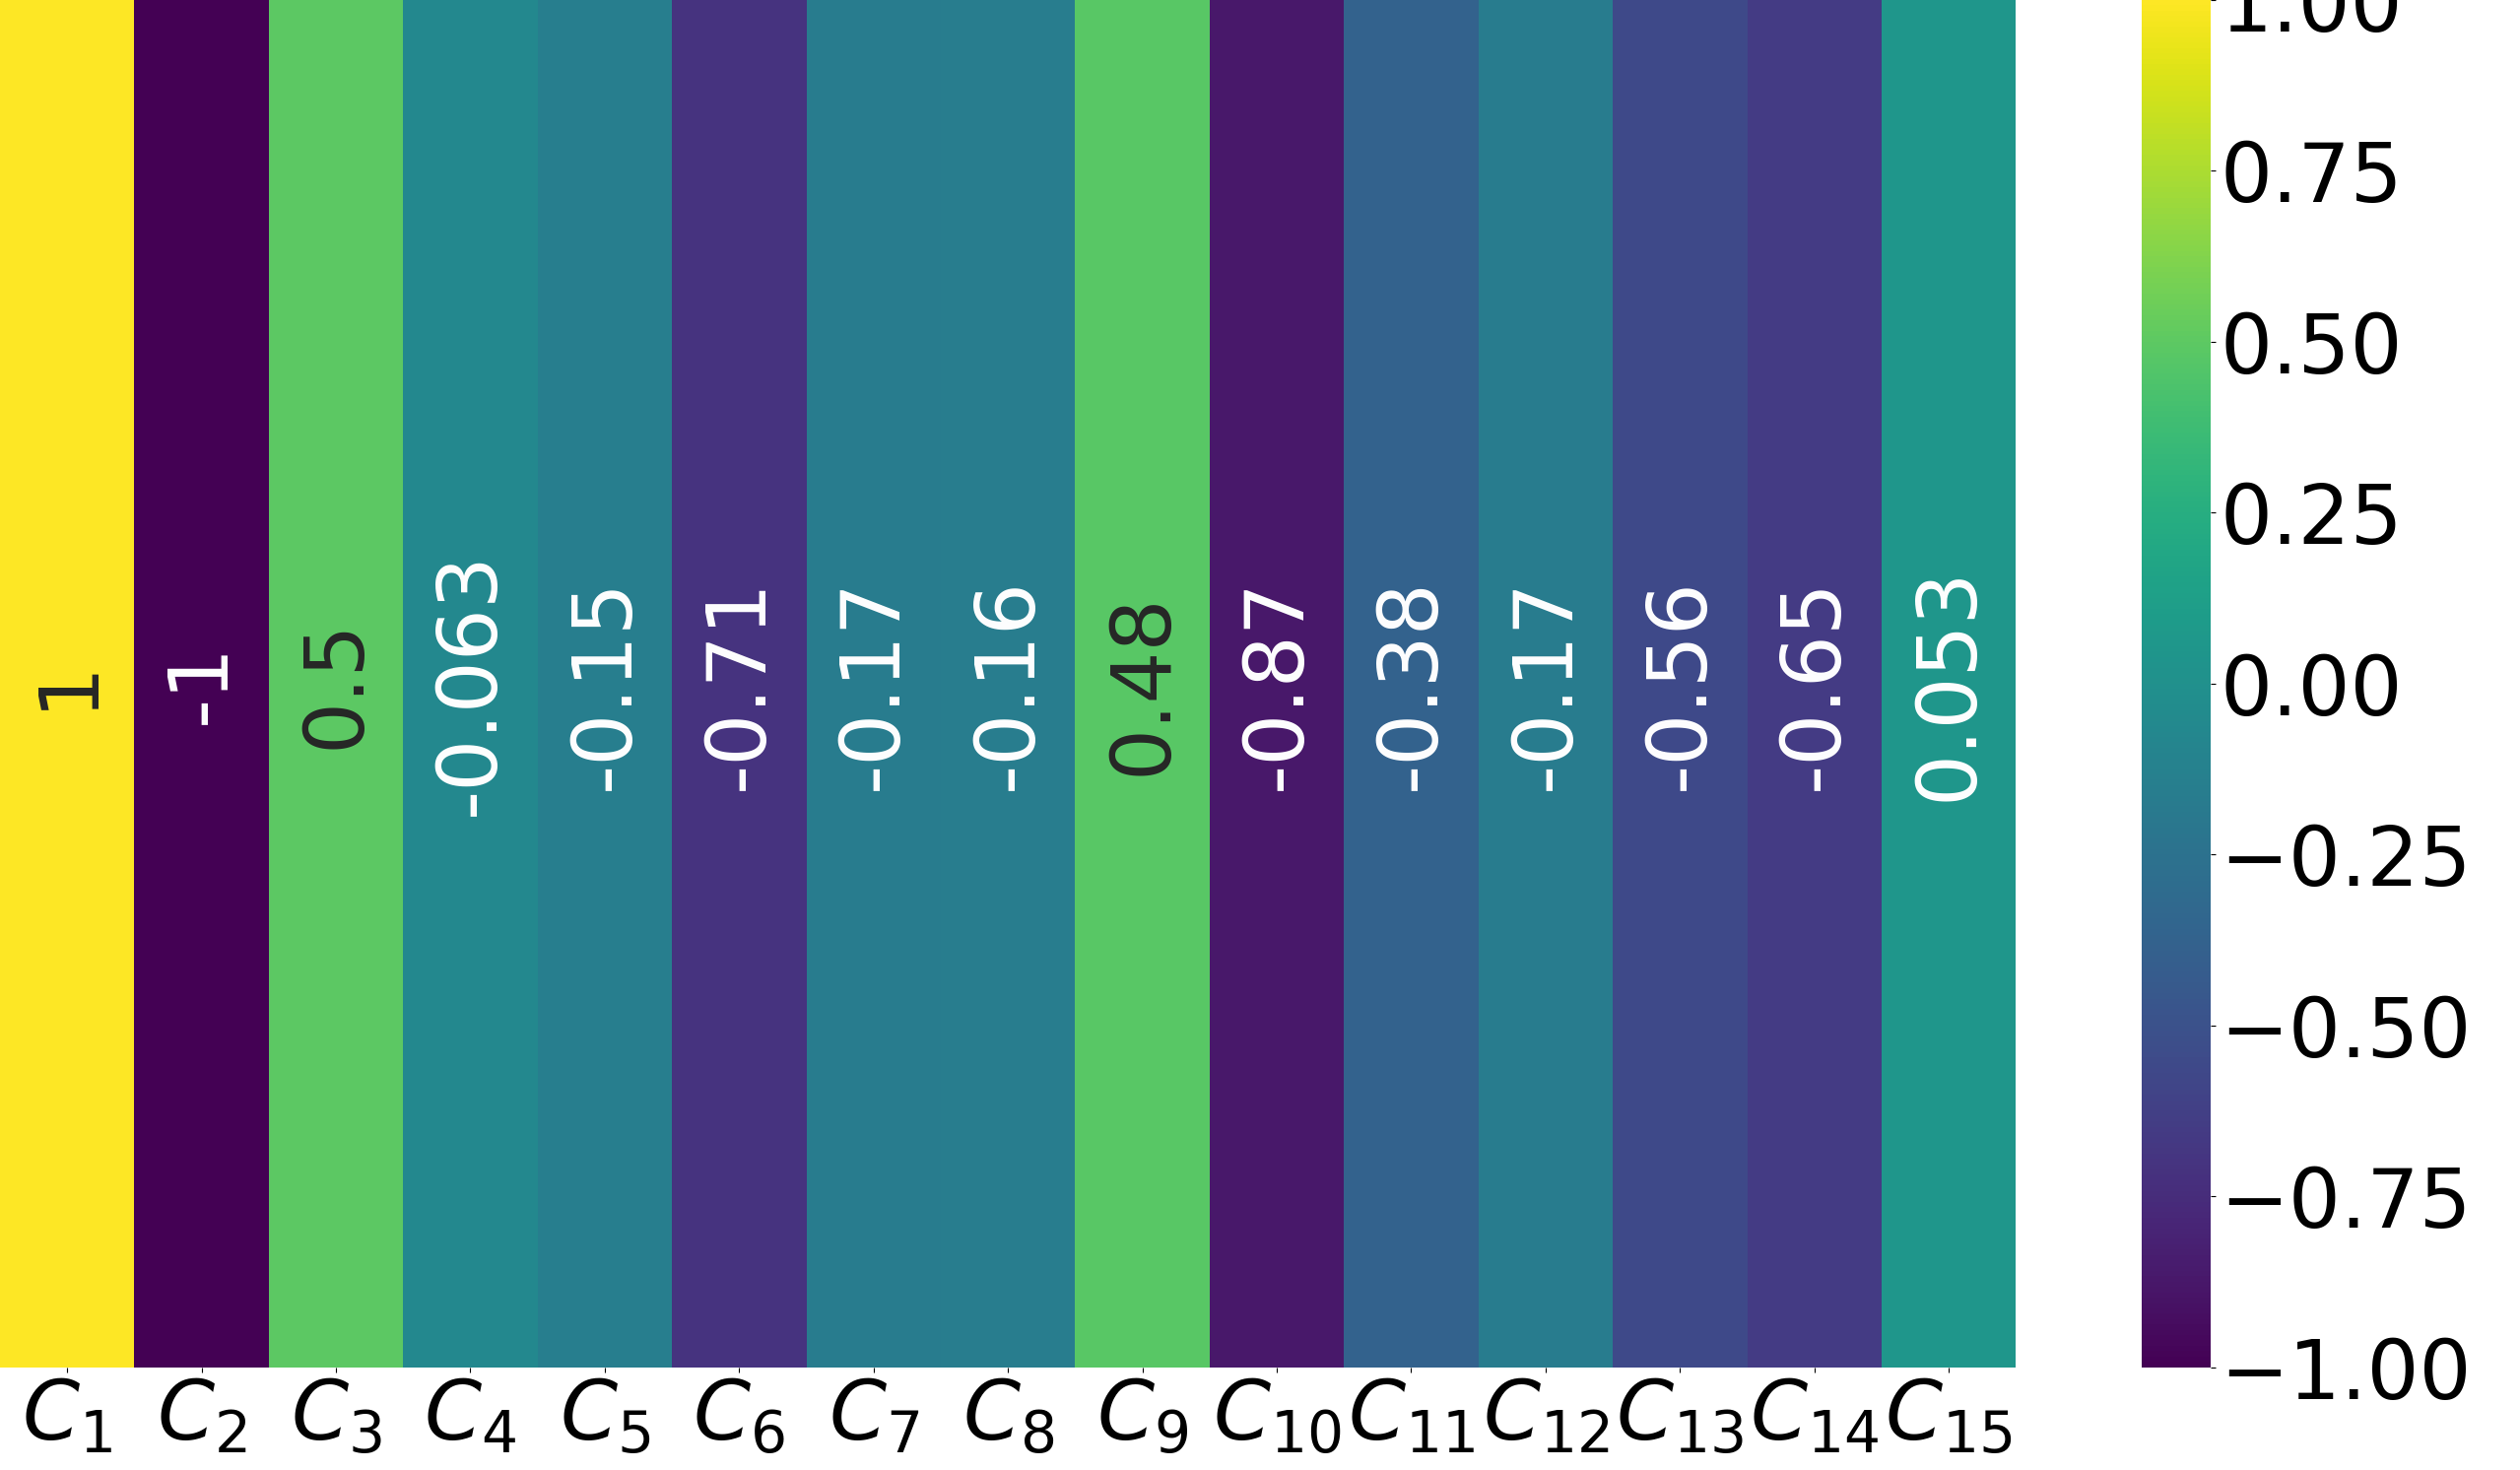
\includegraphics[width=\linewidth]{img/qlp_corr/Cnmod_coil1.png}
		\subcaption{Correlation with coil $1$}
	\end{subfigure}
	\begin{subfigure}{0.49\linewidth}
		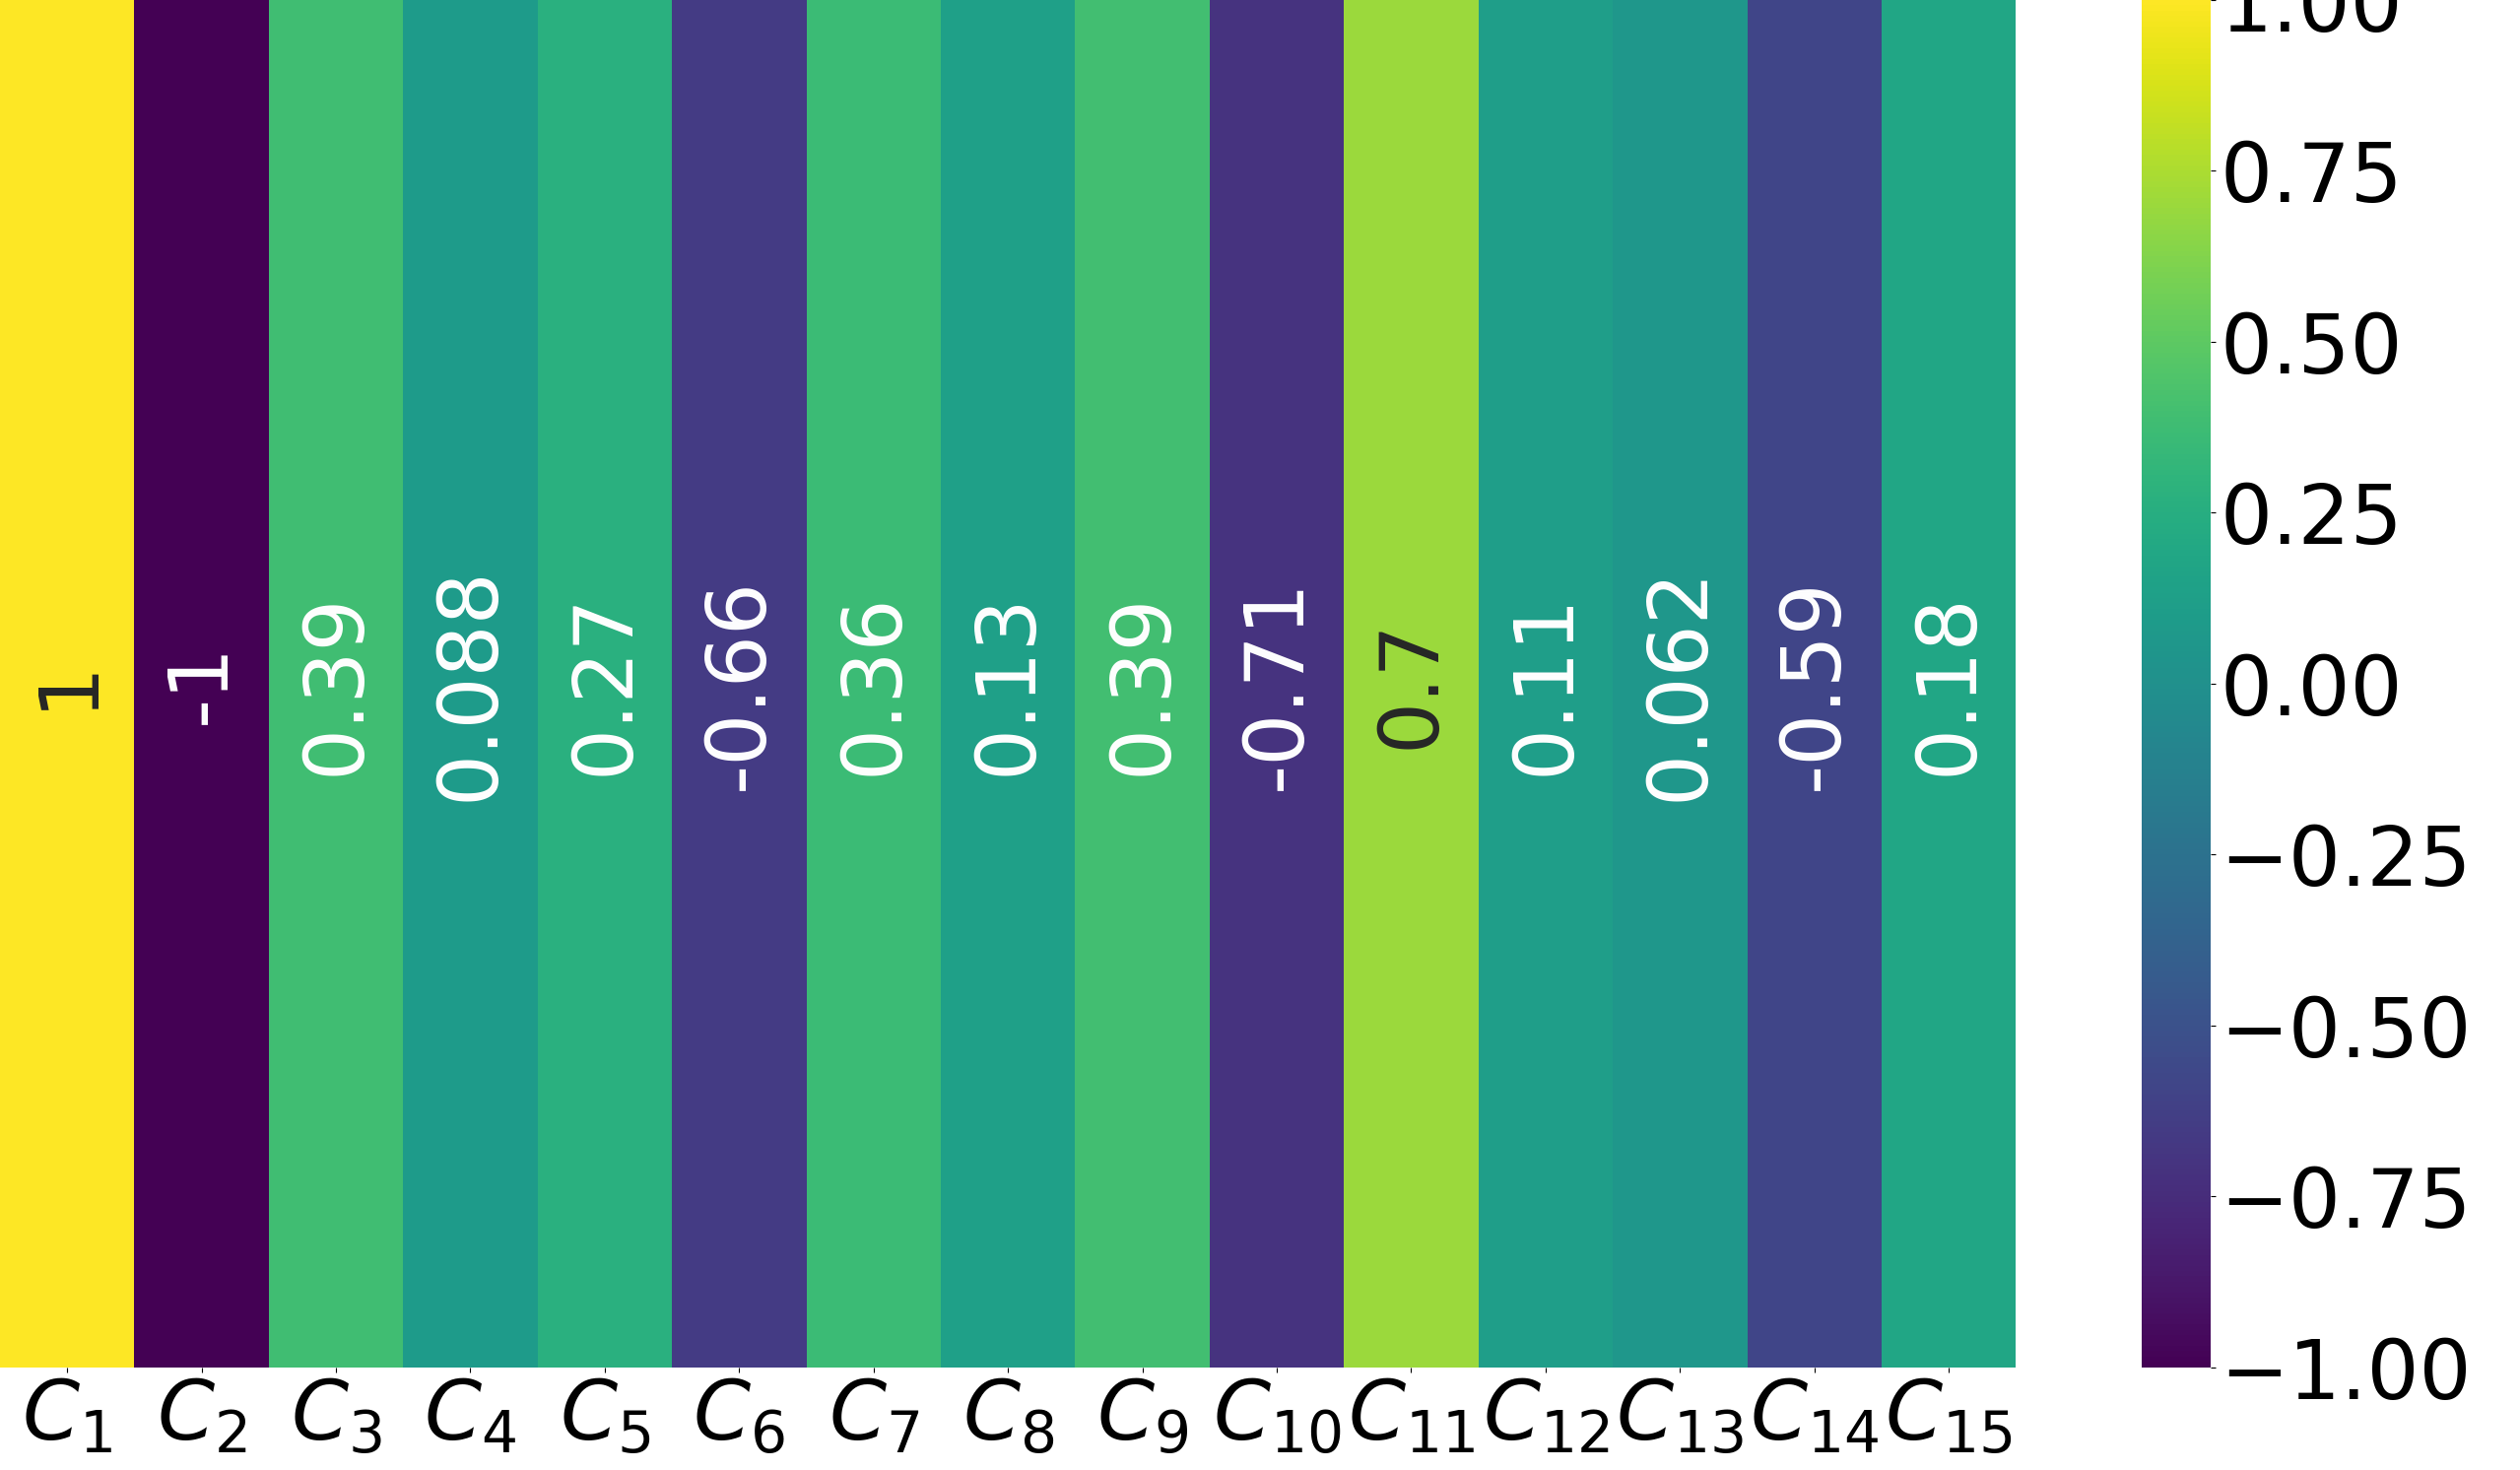
\includegraphics[width=\linewidth]{img/qlp_corr/Cnmod_coil2.png}
		\subcaption{Correlation with coil $2$}
	\end{subfigure}
	\begin{subfigure}{0.49\linewidth}
		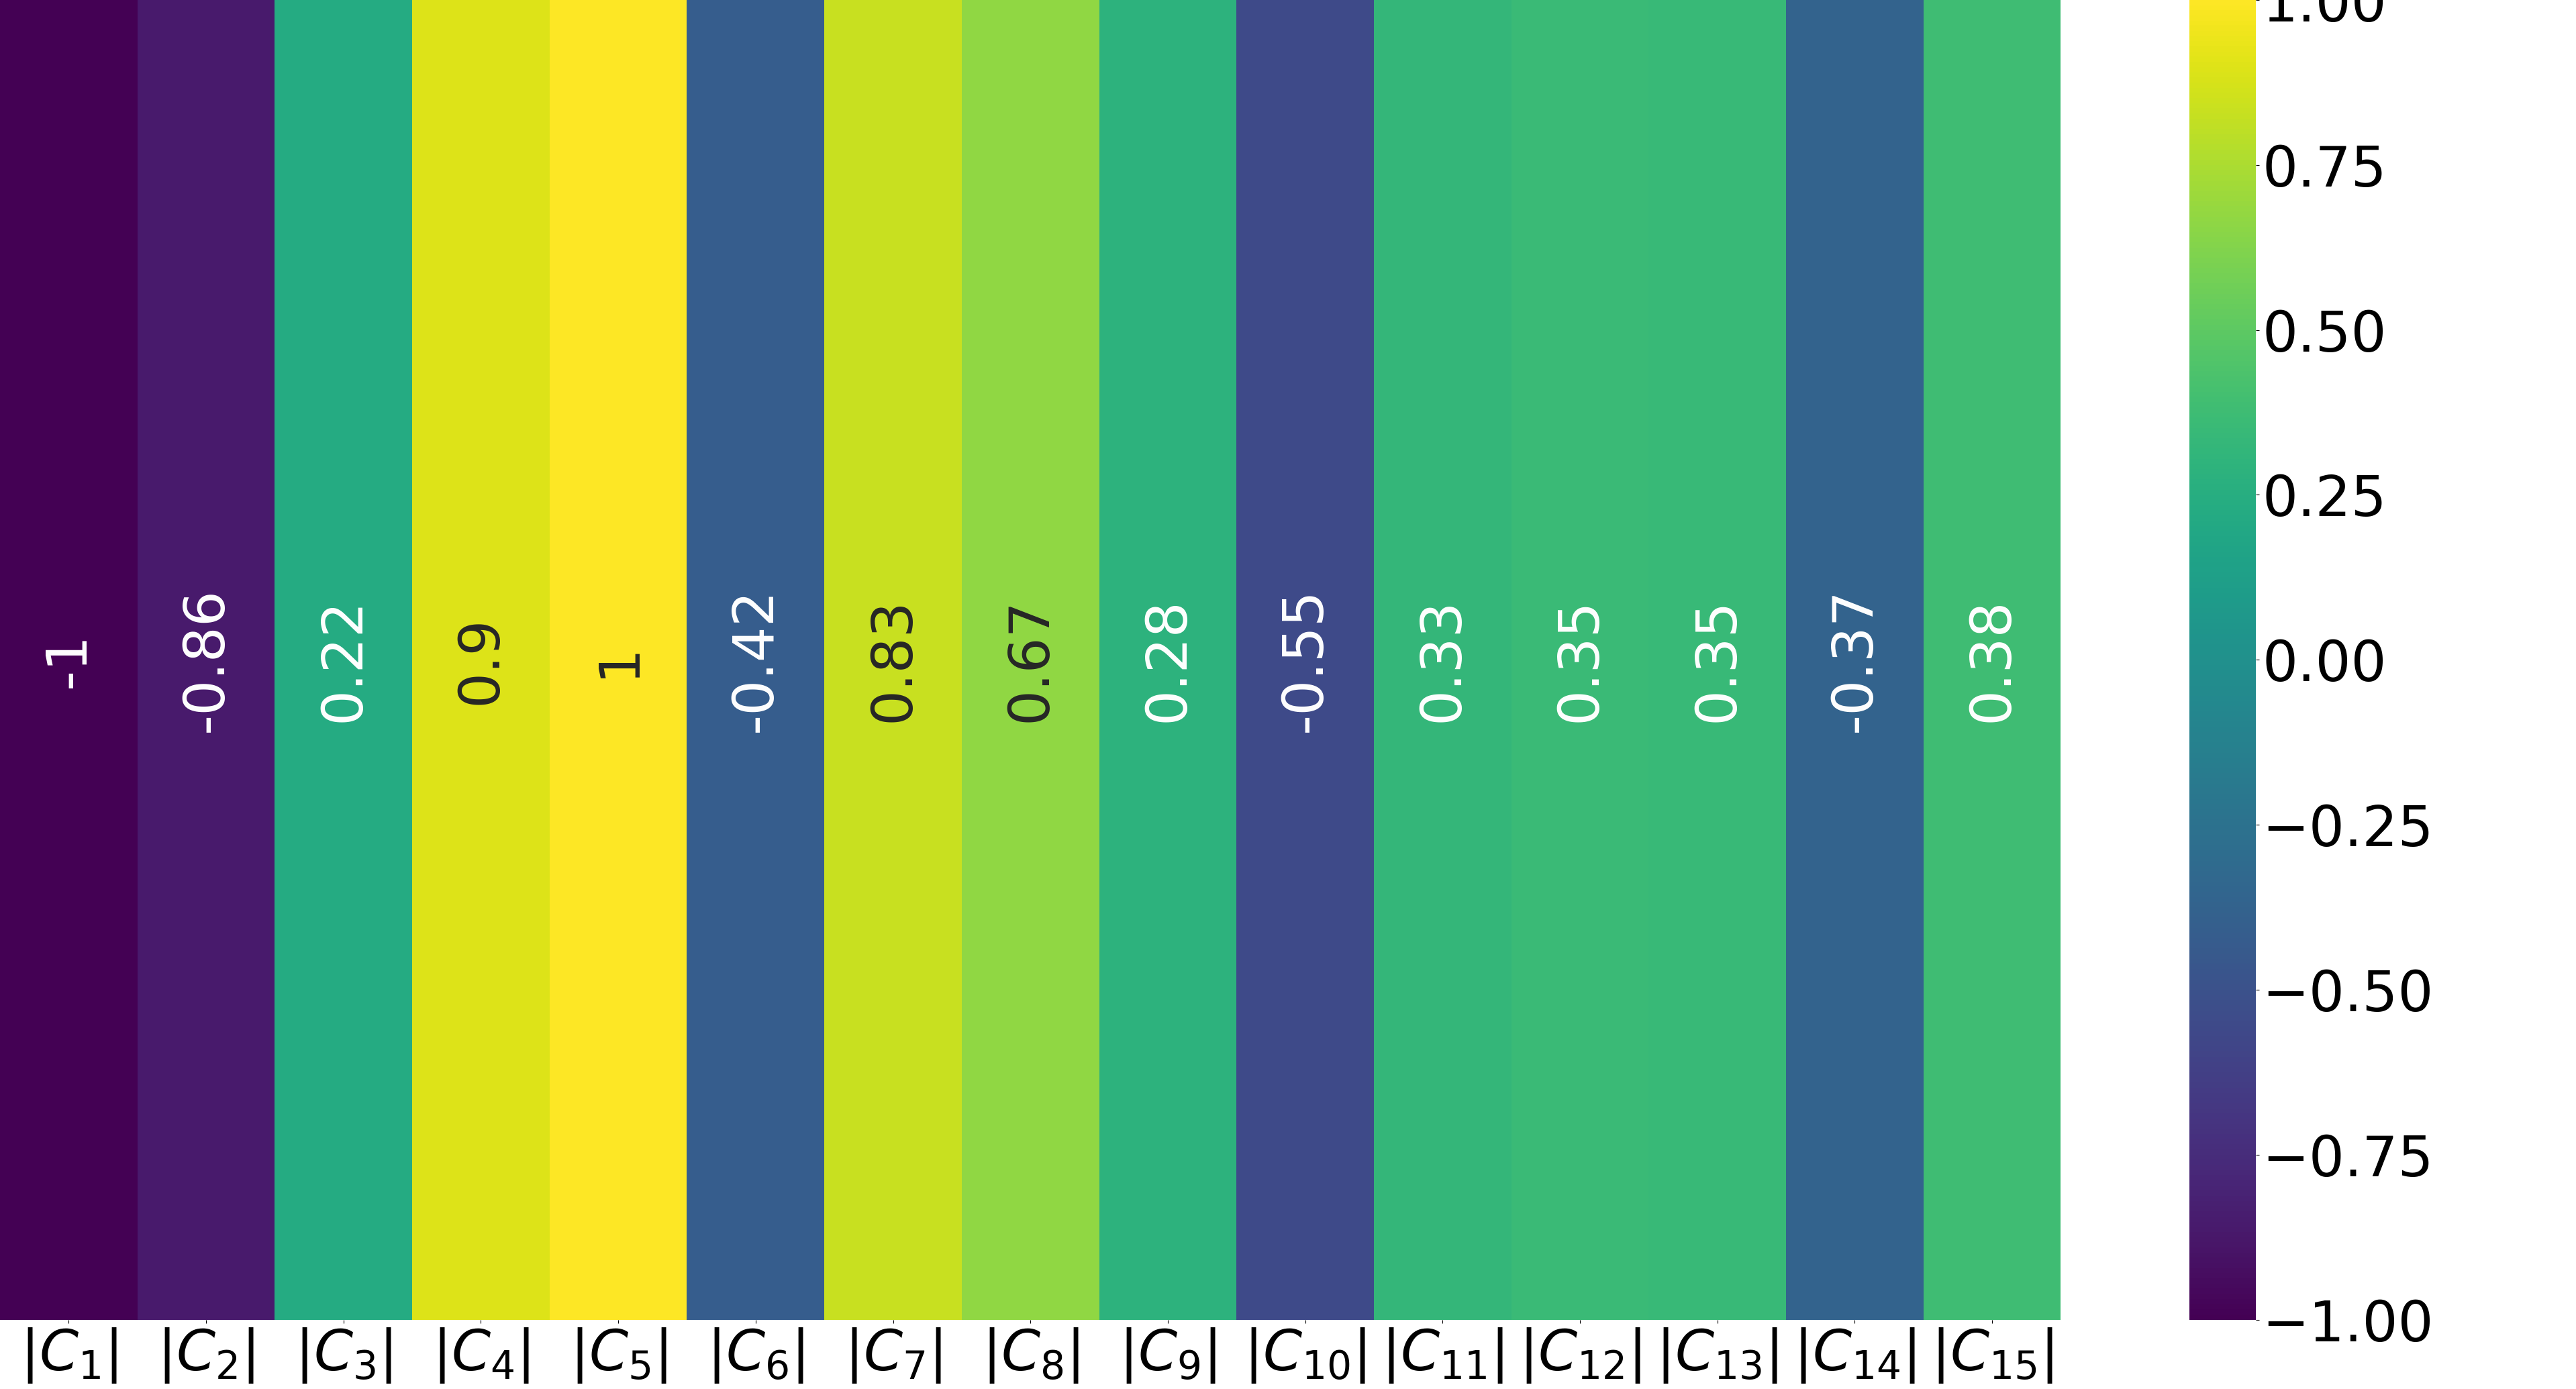
\includegraphics[width=\linewidth]{img/qlp_corr/Cnmod_coil3.png}
		\subcaption{Correlation with coil $3$}
	\end{subfigure}
	\caption{Correlation between the harmonics of the \cnmod\ attribute and the labels for \qlp.}
	\label{fig:cnmod-lcorr-qlp}
\end{figure}

As we did for \an\ and \bn, we visualized \cnmod\ after a round of \pca\ dimensionality reduction.
\Cref{fig:cnmod-coilq-dist} shows a similar situation to \an, if we consider the specific case of
sub-figure (a), while the clusters are not as clean cut as the alternative, there is much more
separation of the classes compared to \bn. As far as single coil quench is concerned (cfr. sub-figure
(b)), there is clearly a high degree of homogeneity due to having many groups of points labelled
differently but extremely close together.
\begin{figure}[!ht]
	% Font size = 40
	\centering
	\begin{subfigure}{0.8\linewidth}
		\centering
		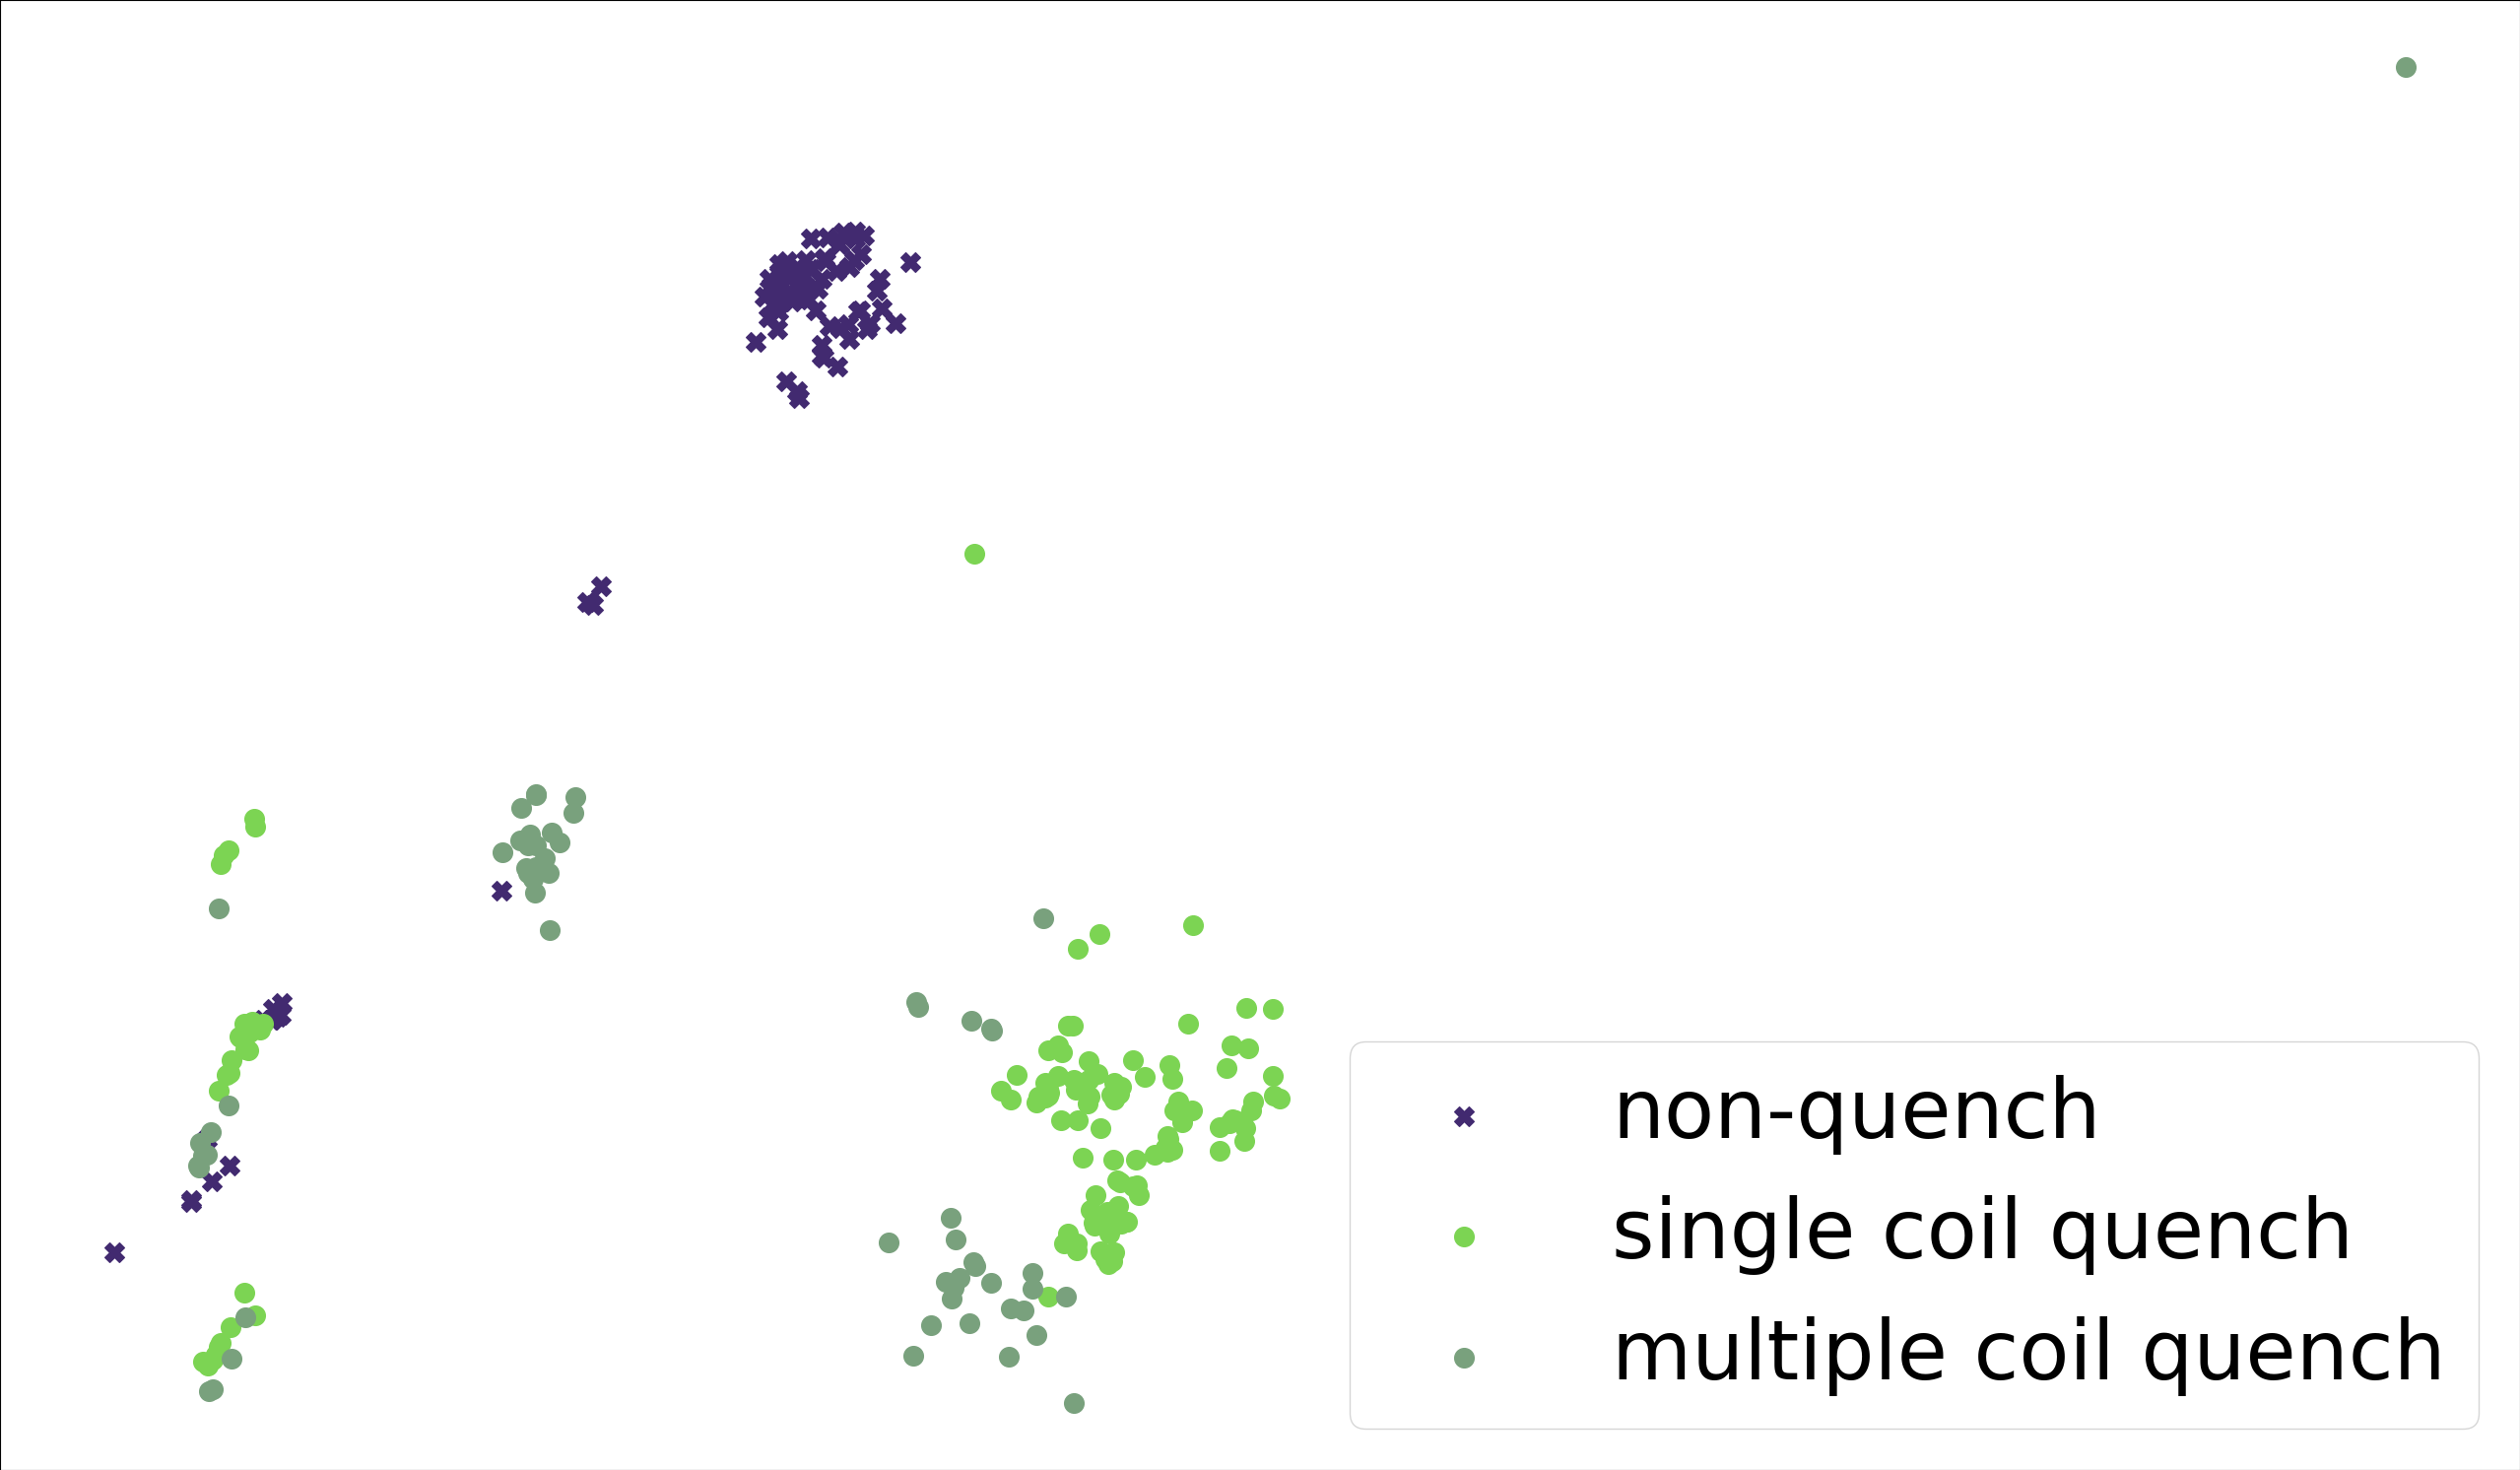
\includegraphics[width=\linewidth]{img/quench_dist_qlp/single_vs_multiple_Cnmod.png}
		\subcaption{}
	\end{subfigure}
	\begin{subfigure}{0.8\linewidth}
		\centering
		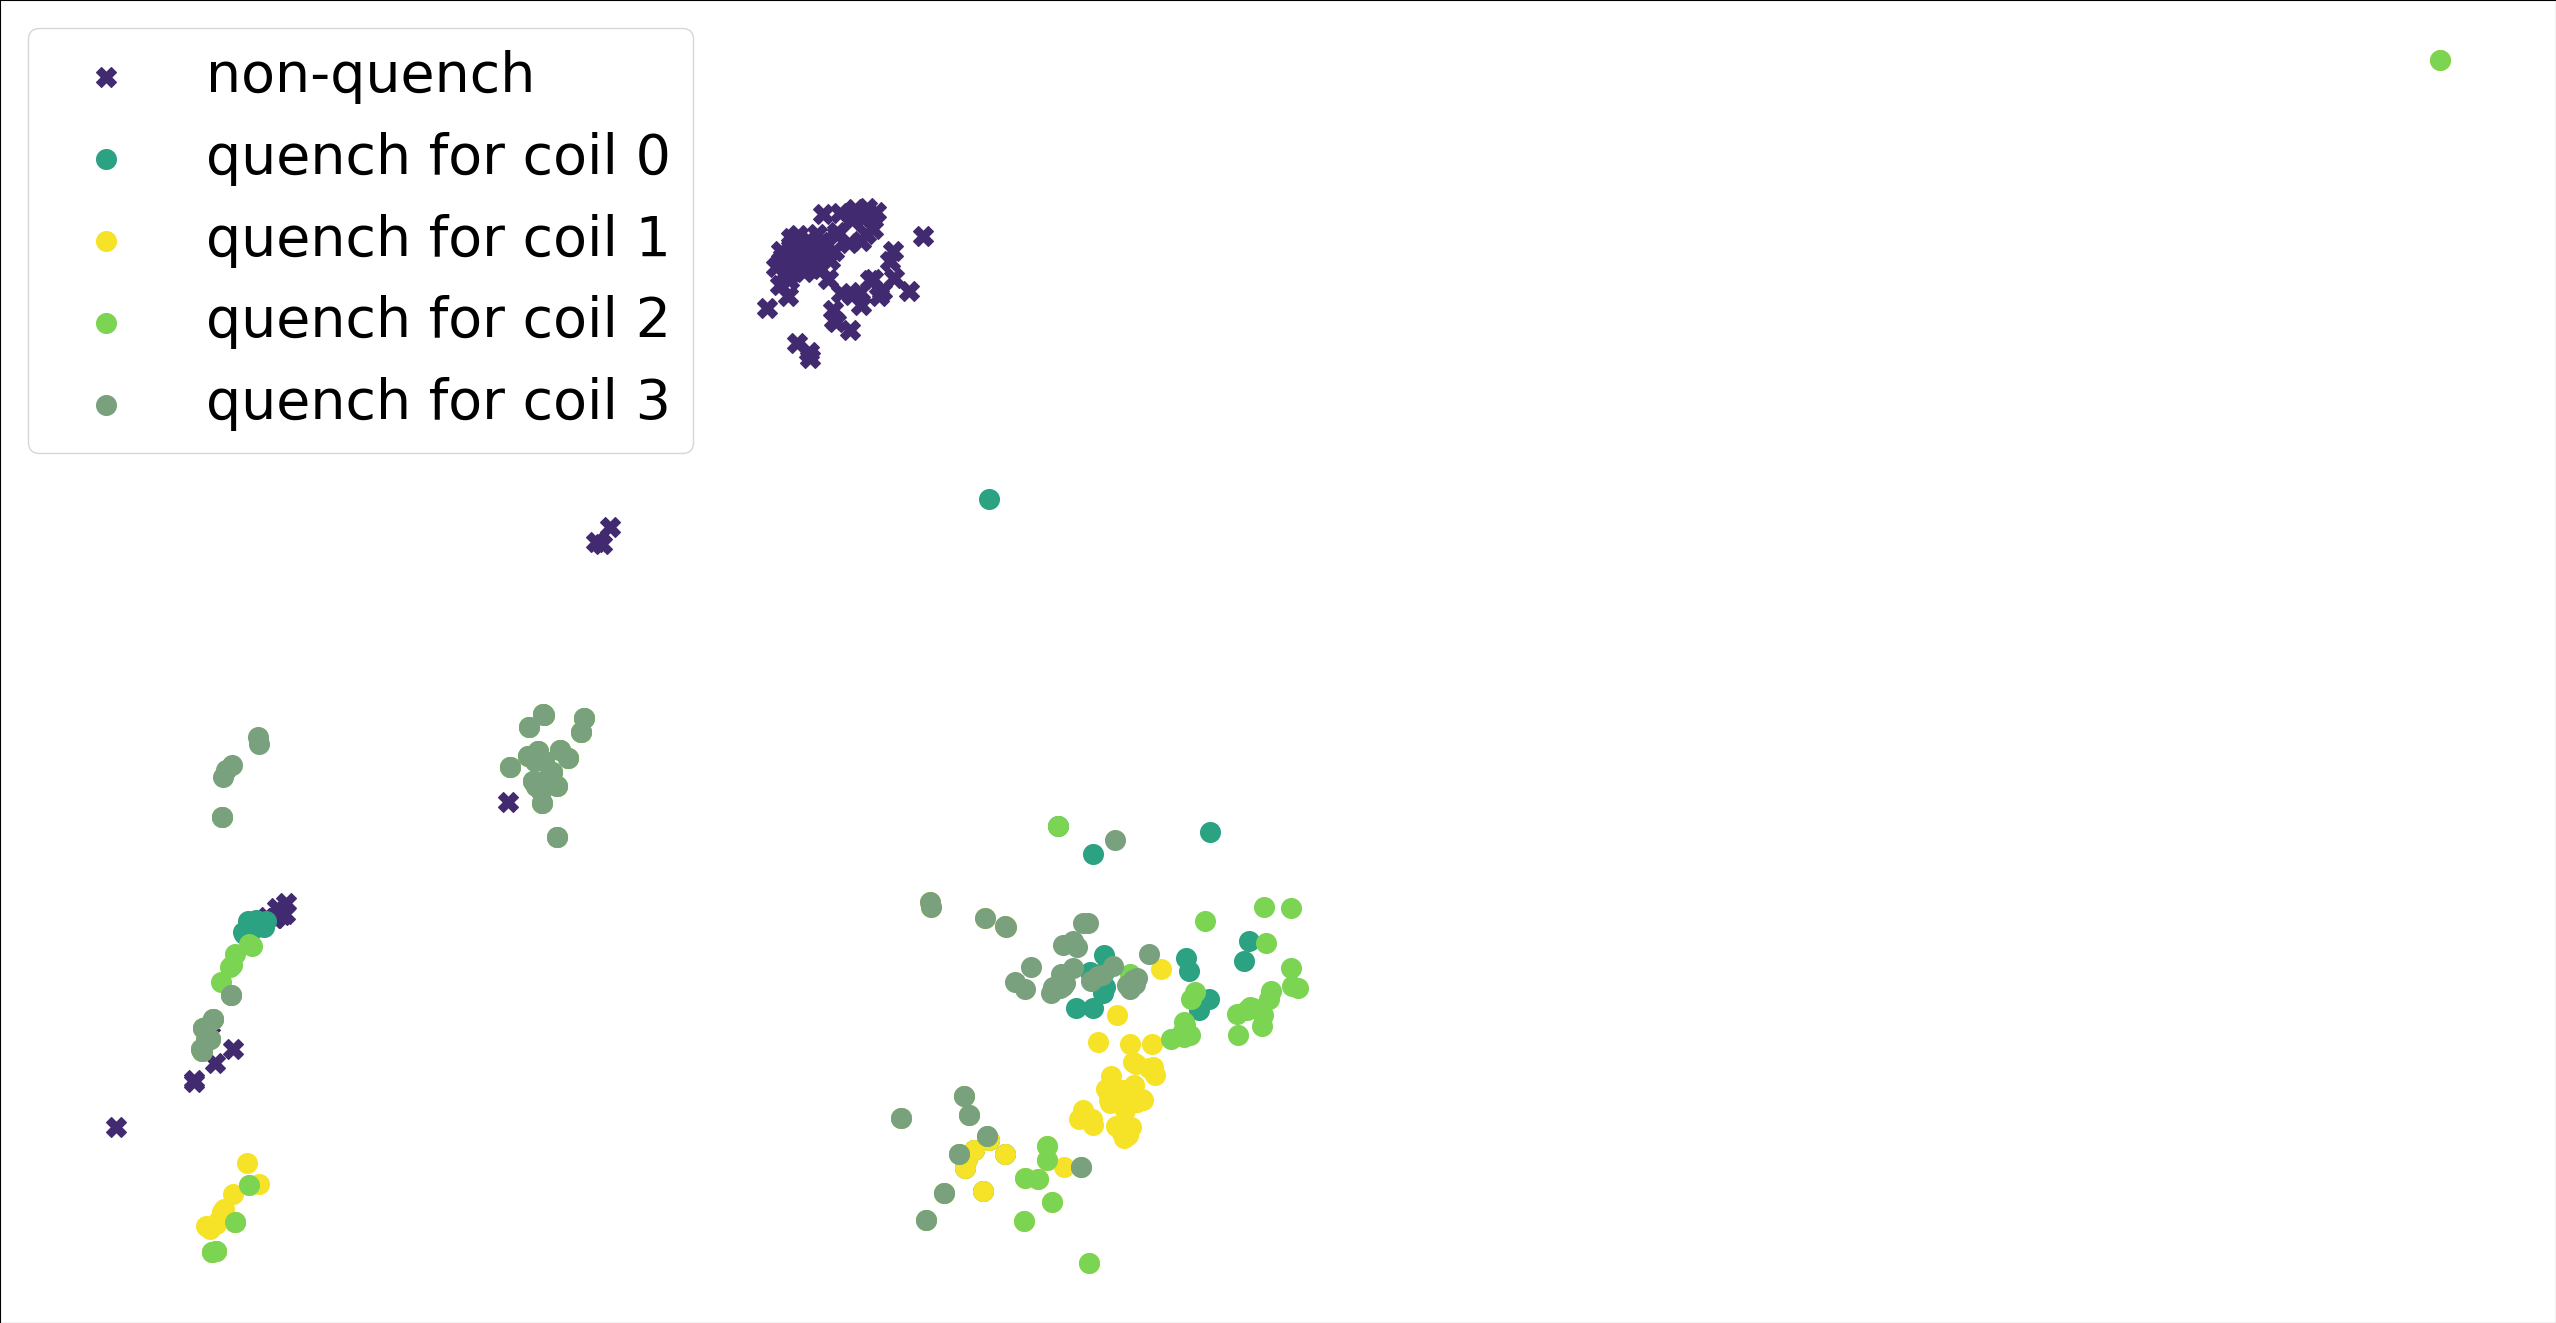
\includegraphics[width=\linewidth]{img/quench_dist_qlp_cnmod.png}
		\subcaption{}
	\end{subfigure}
	\caption{Visualization of the \cnmod\ attribute, the data was plotted after a run of \pca\
		dimensionality reduction. Sub-figure (a) highlights the samples based on how many quenches
		are associated to the specific sample $\{0, 1, \text{many}\}$. Sub-figure (b) highlights the
		samples based on the specific coil quenched $\{\text{None}, 0, 1, 2, 3\}$.}
	\label{fig:cnmod-coilq-dist}
\end{figure}

\subsubsection{\phin}
To close the section we are going to consider the \phin\ attribute. In \Cref{fig:phi-lcorr-qlp} we
plotted the cross-correlation between the harmonics and the labels. Due to how high the correlation
is between most harmonics and basically all the coils, we might be lead to think that this is the
best attribute available to us. Since the harmonics are also very weakly correlated among themselves
(cfr. \Cref{fig:phi-corr}), we just chose to not extract any features and keep the attribute as is.
On the other hand, the bidimensional visualization of the data is telling a different story (cfr.
\Cref{fig:phi-coilq-dist}), closer, as a matter of fact, to what we discovered for \bn.

\Cref{fig:phi-coilq-dist} plots the data after a round of \pca\ dimensionality reduction.
Independently of the sub-figure we consider, the sparsity and the homogeneity of the data makes it
extremely hard to define clusters with a high level of purity.
\begin{figure}[!ht]
	% Font size = 70
	\centering
	\begin{subfigure}{0.49\linewidth}
		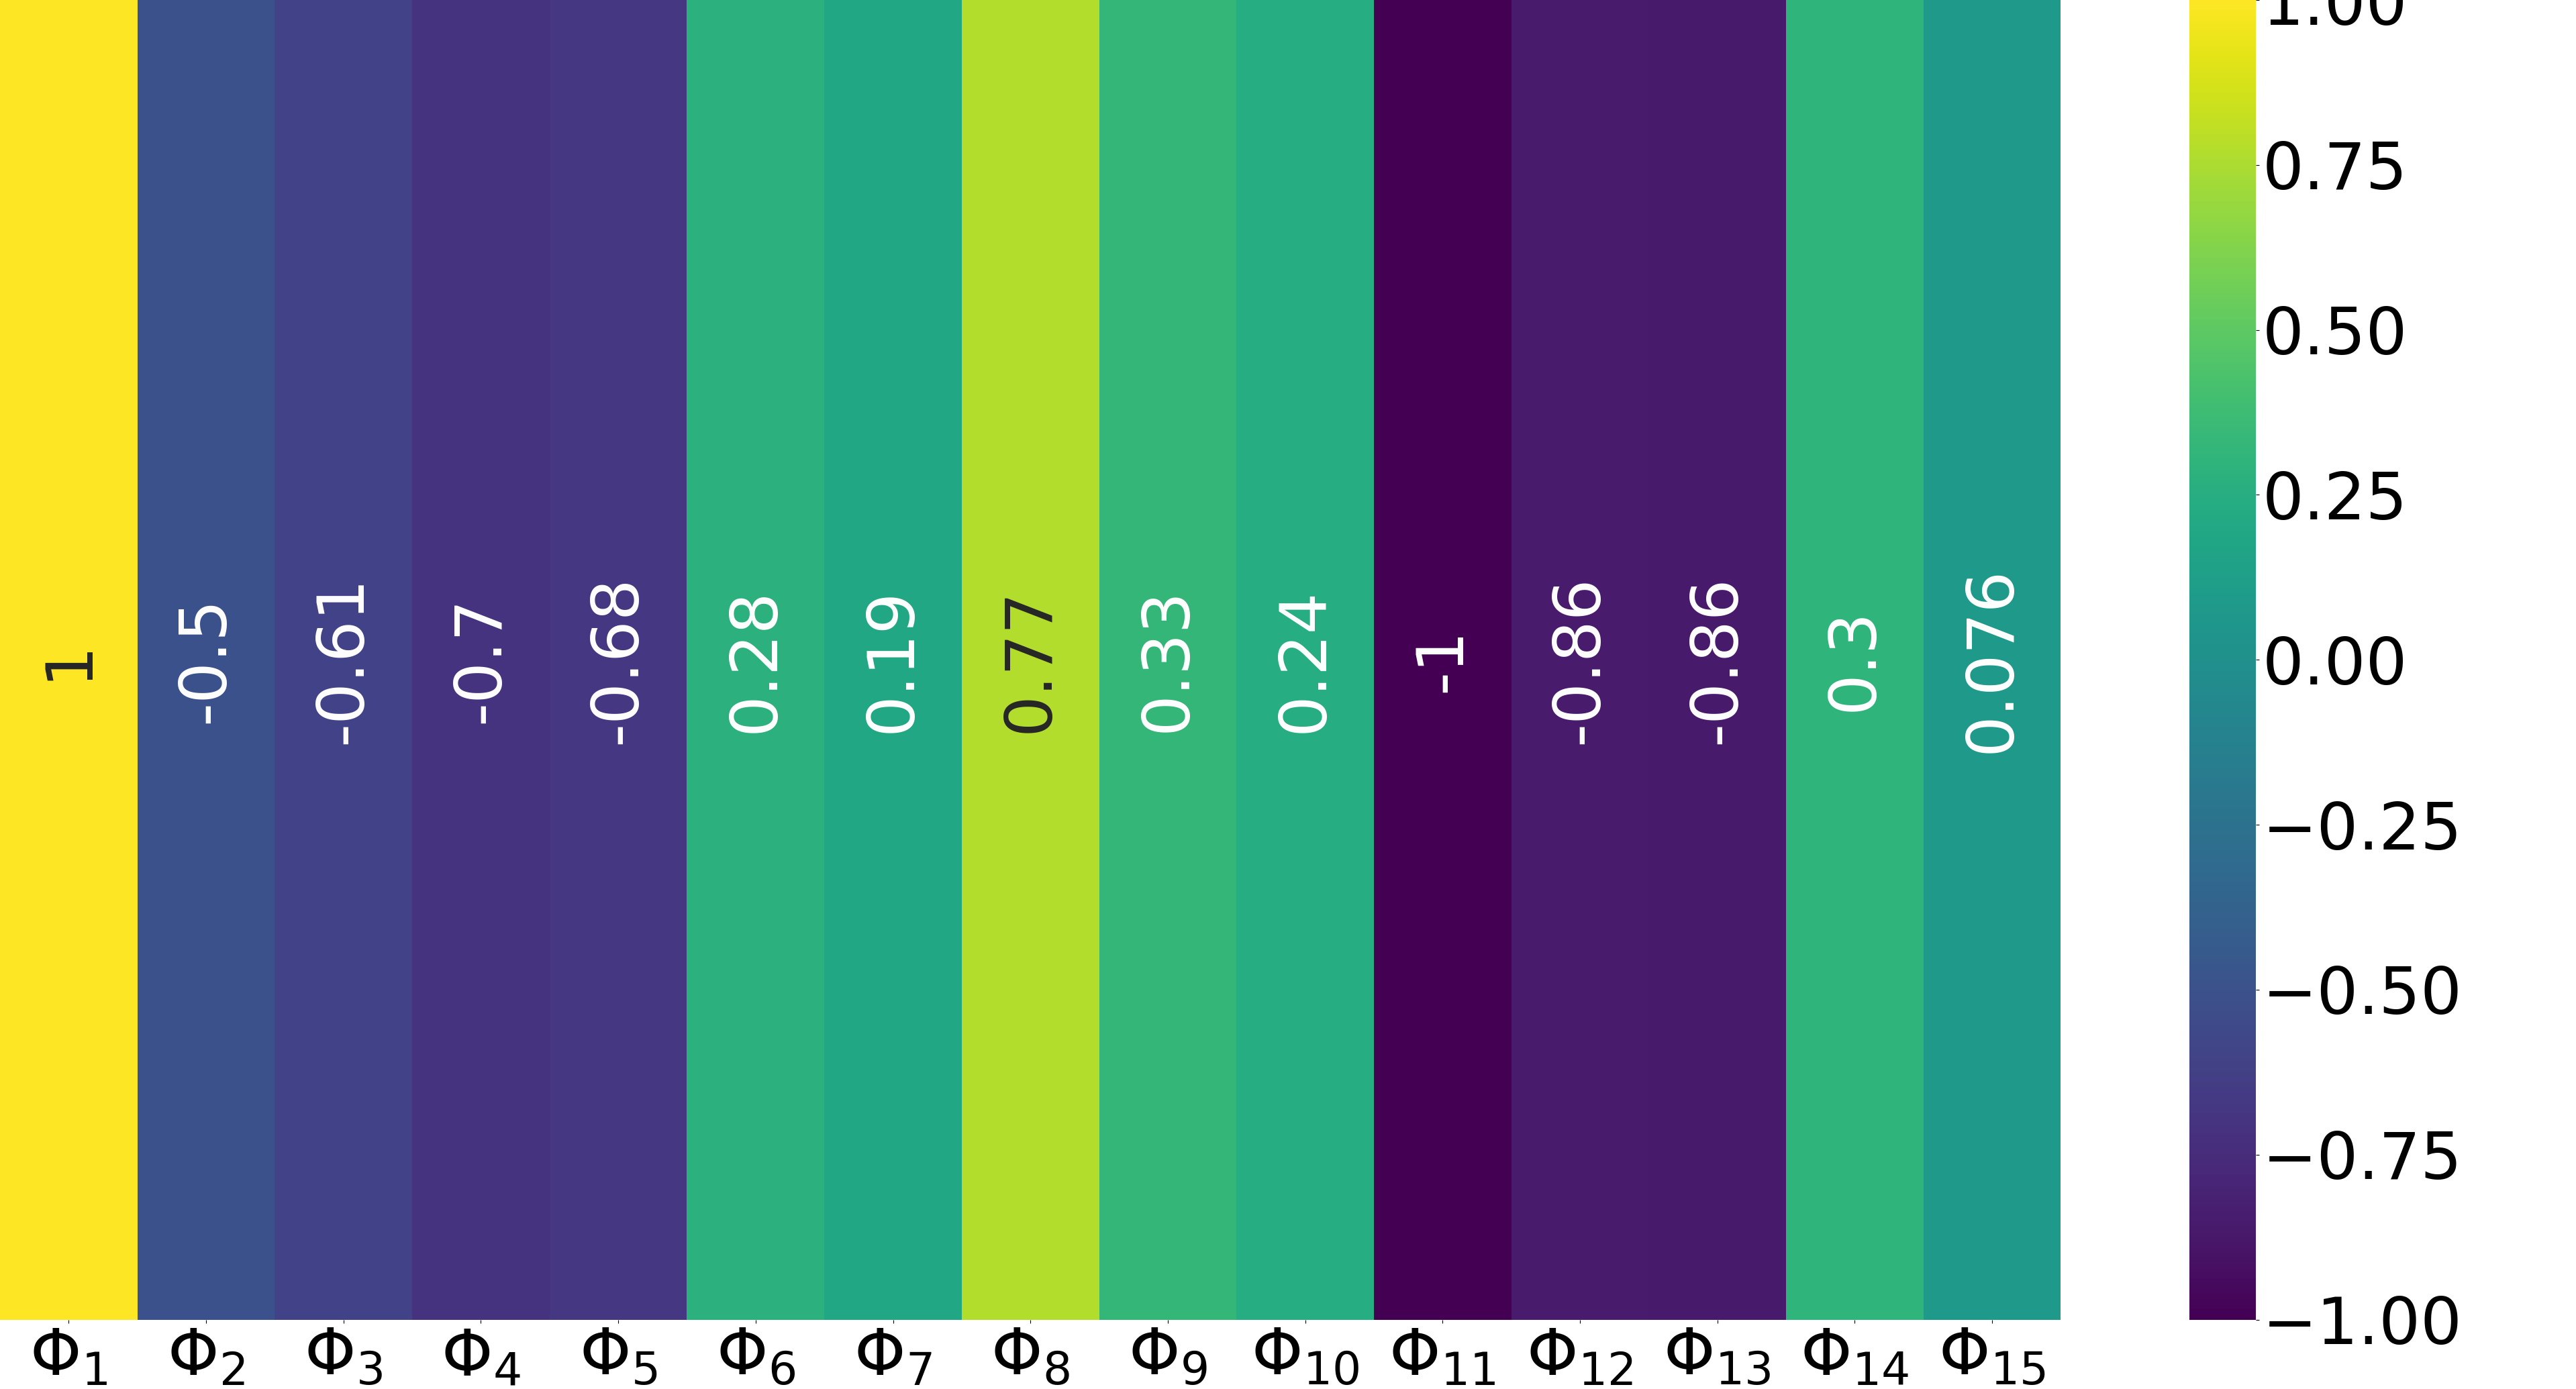
\includegraphics[width=\linewidth]{img/qlp_corr/Phi_coil0.png}
		\subcaption{Correlation with coil $0$}
	\end{subfigure}
	\begin{subfigure}{0.49\linewidth}
		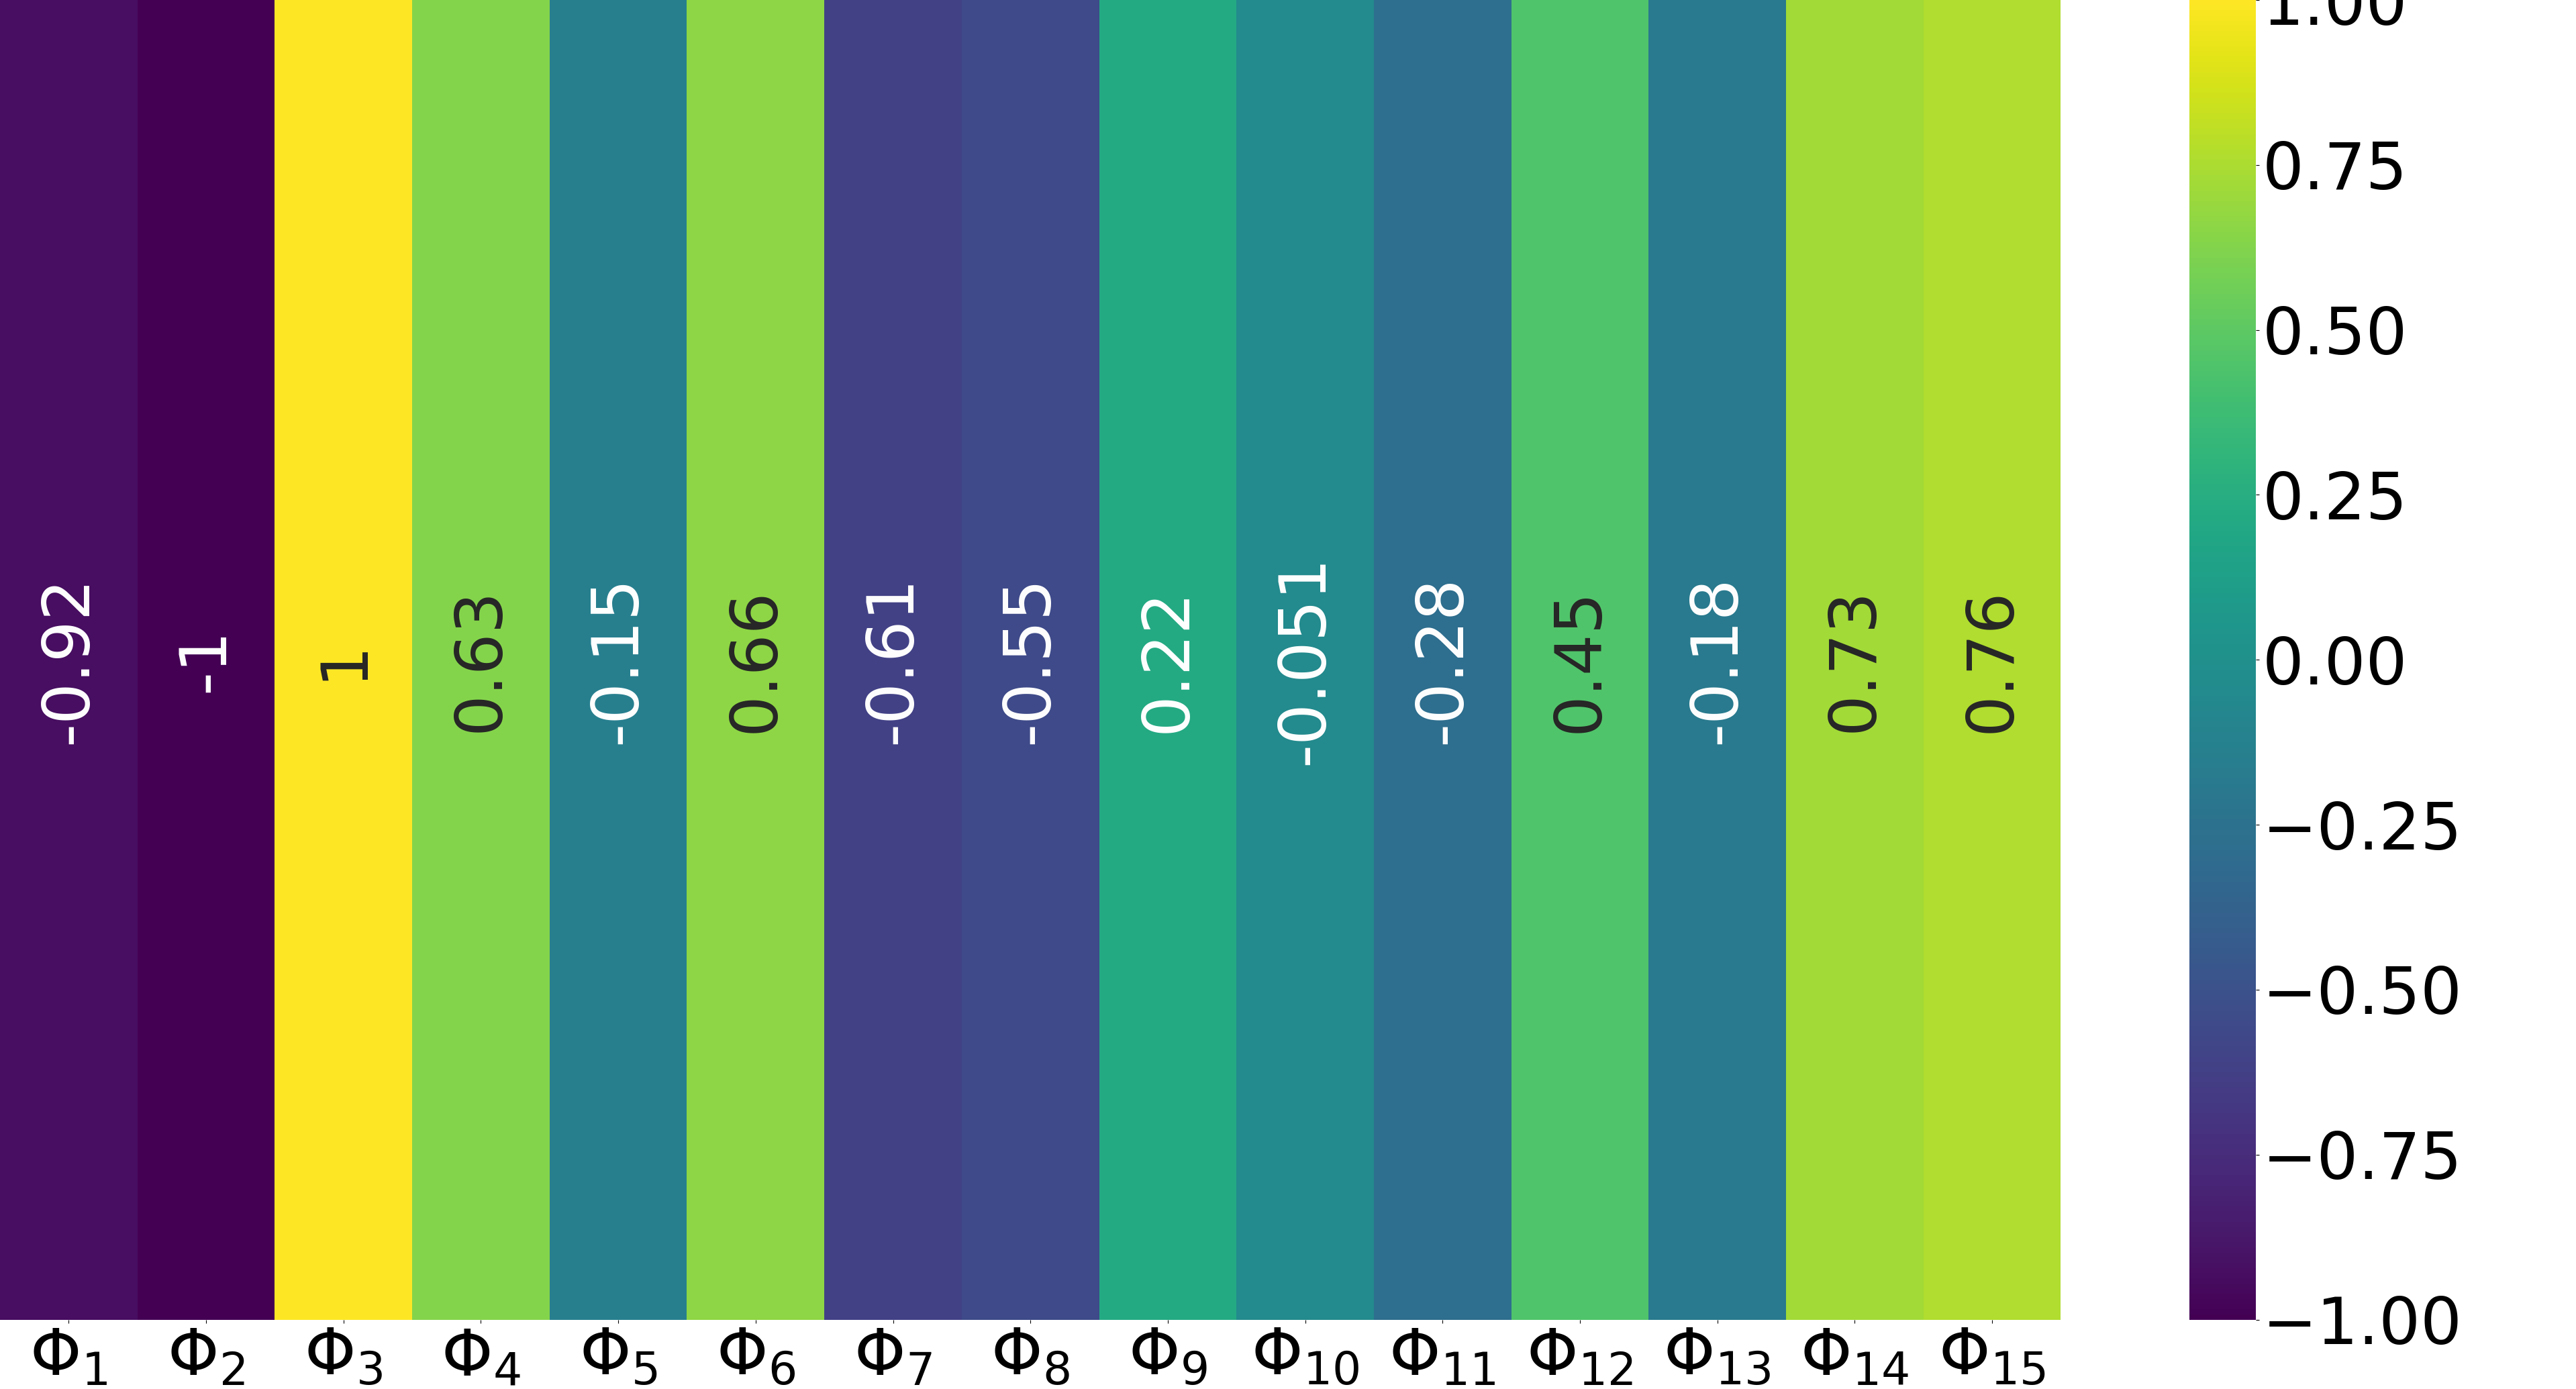
\includegraphics[width=\linewidth]{img/qlp_corr/Phi_coil1.png}
		\subcaption{Correlation with coil $1$}
	\end{subfigure}
	\begin{subfigure}{0.49\linewidth}
		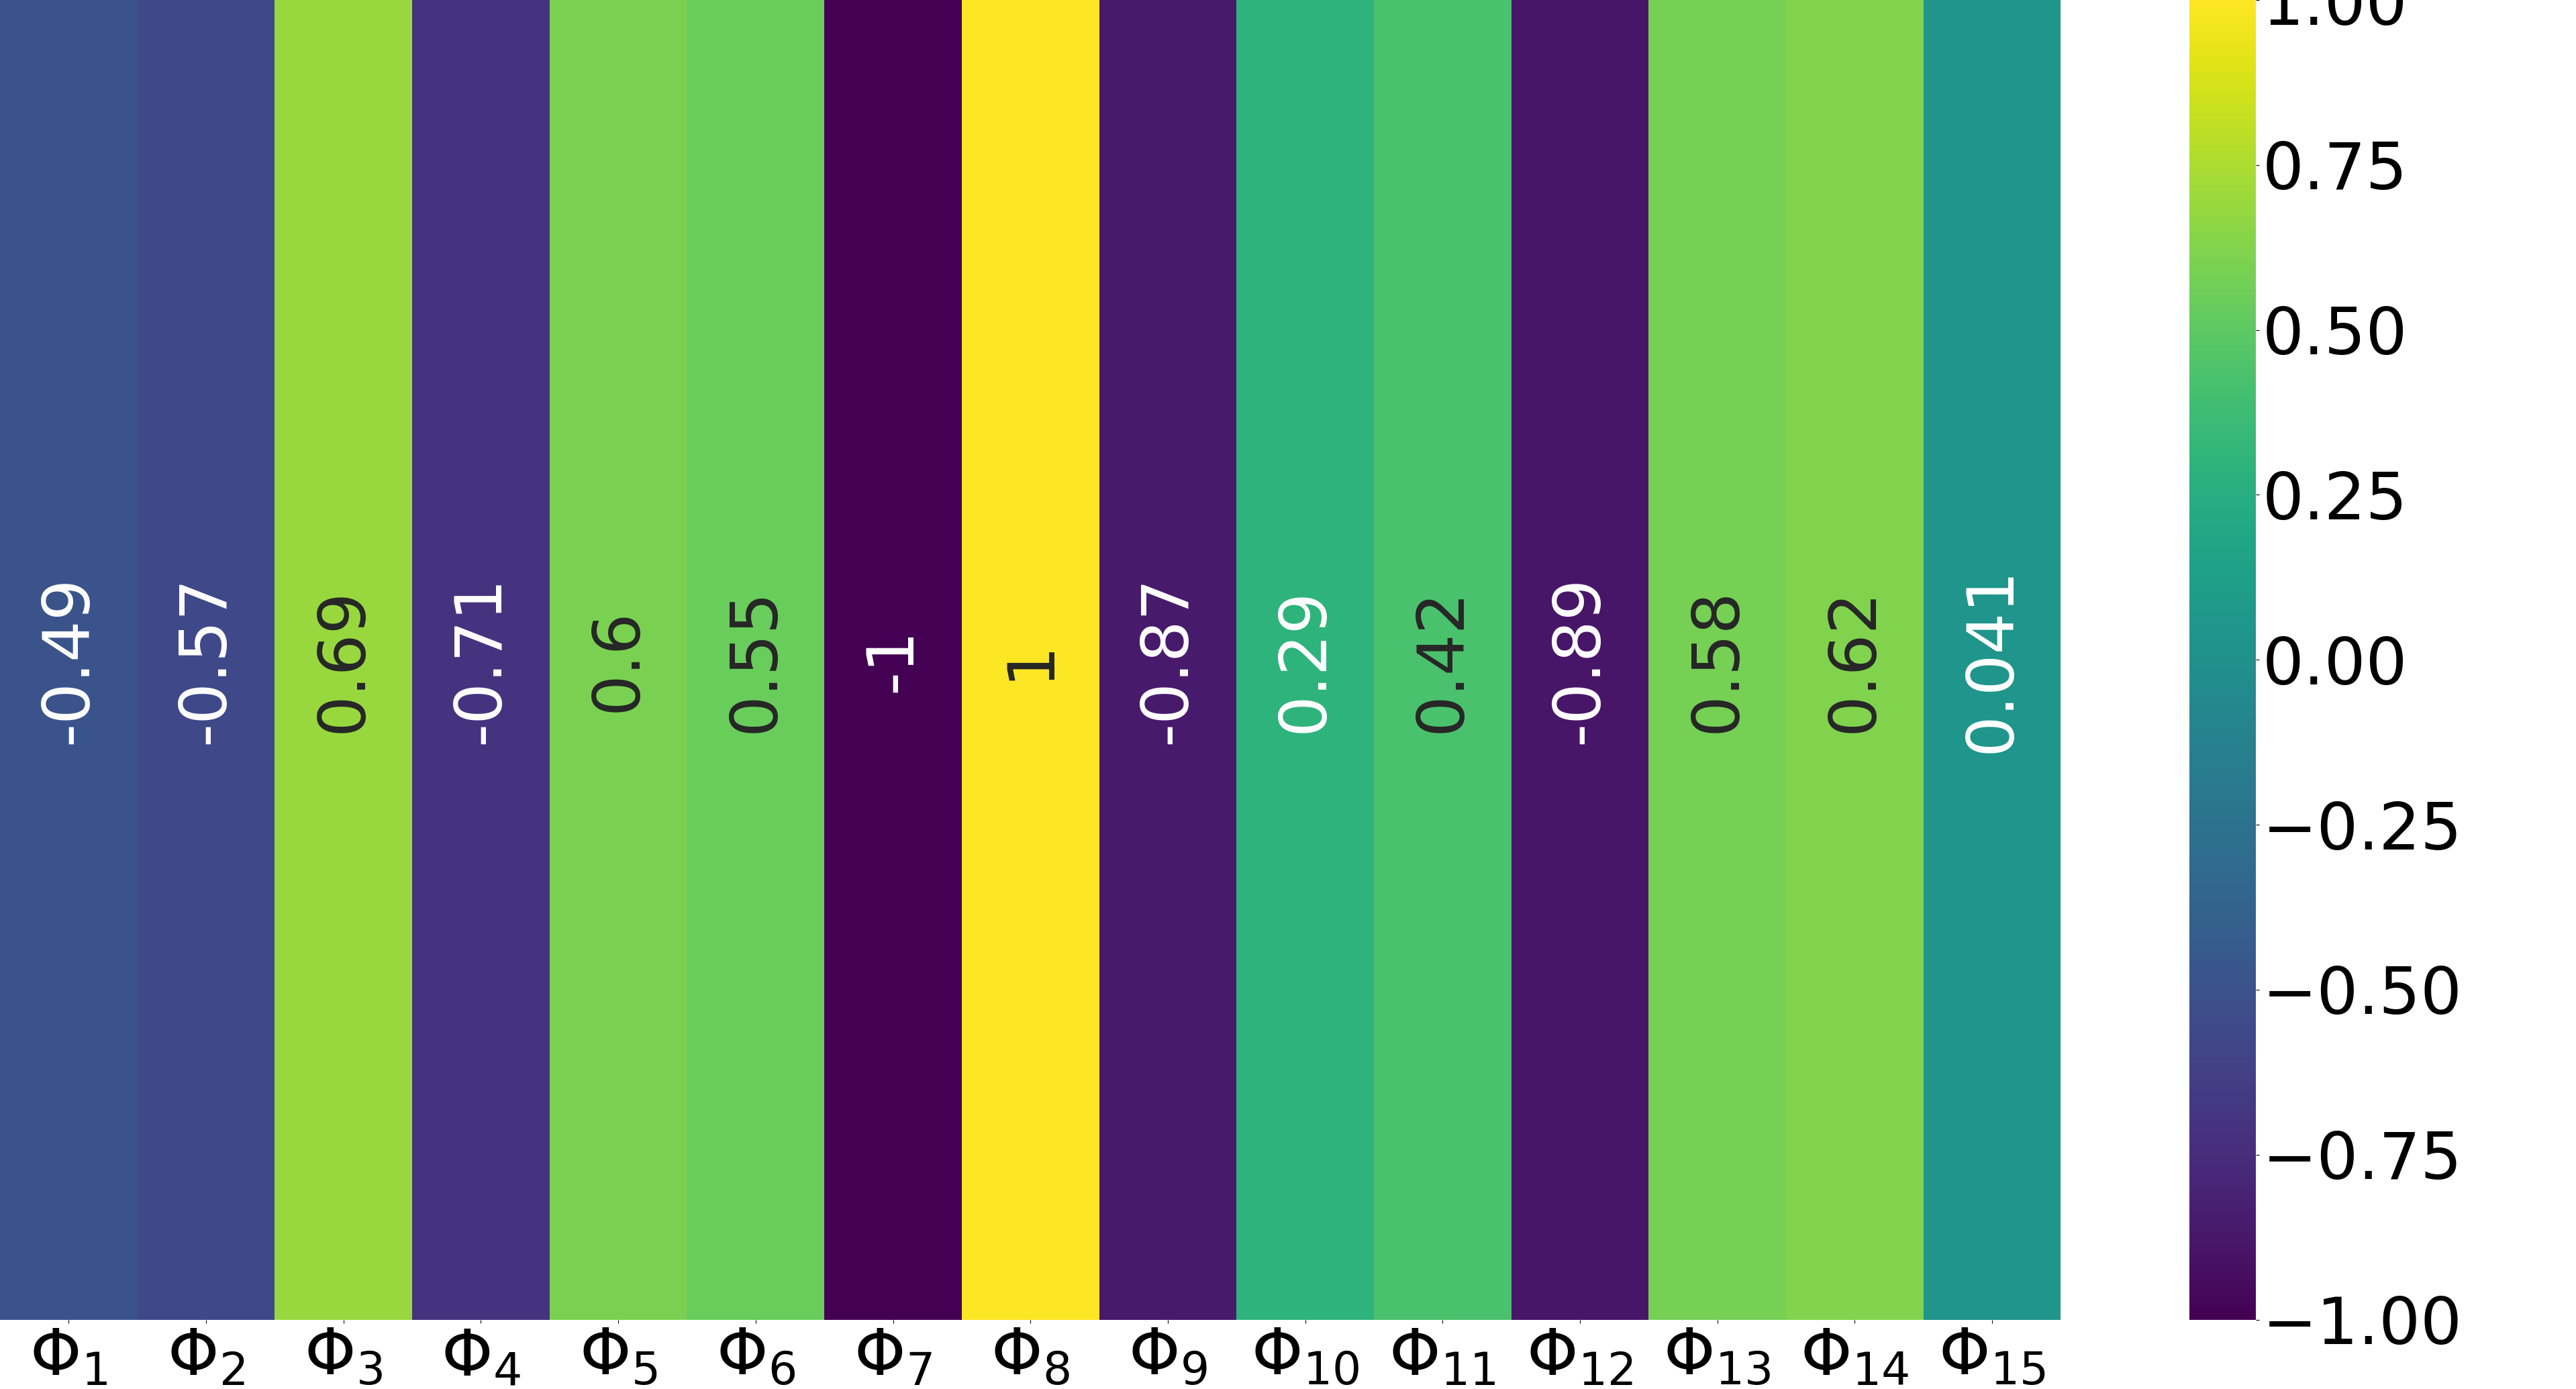
\includegraphics[width=\linewidth]{img/qlp_corr/Phi_coil2.png}
		\subcaption{Correlation with coil $2$}
	\end{subfigure}
	\begin{subfigure}{0.49\linewidth}
		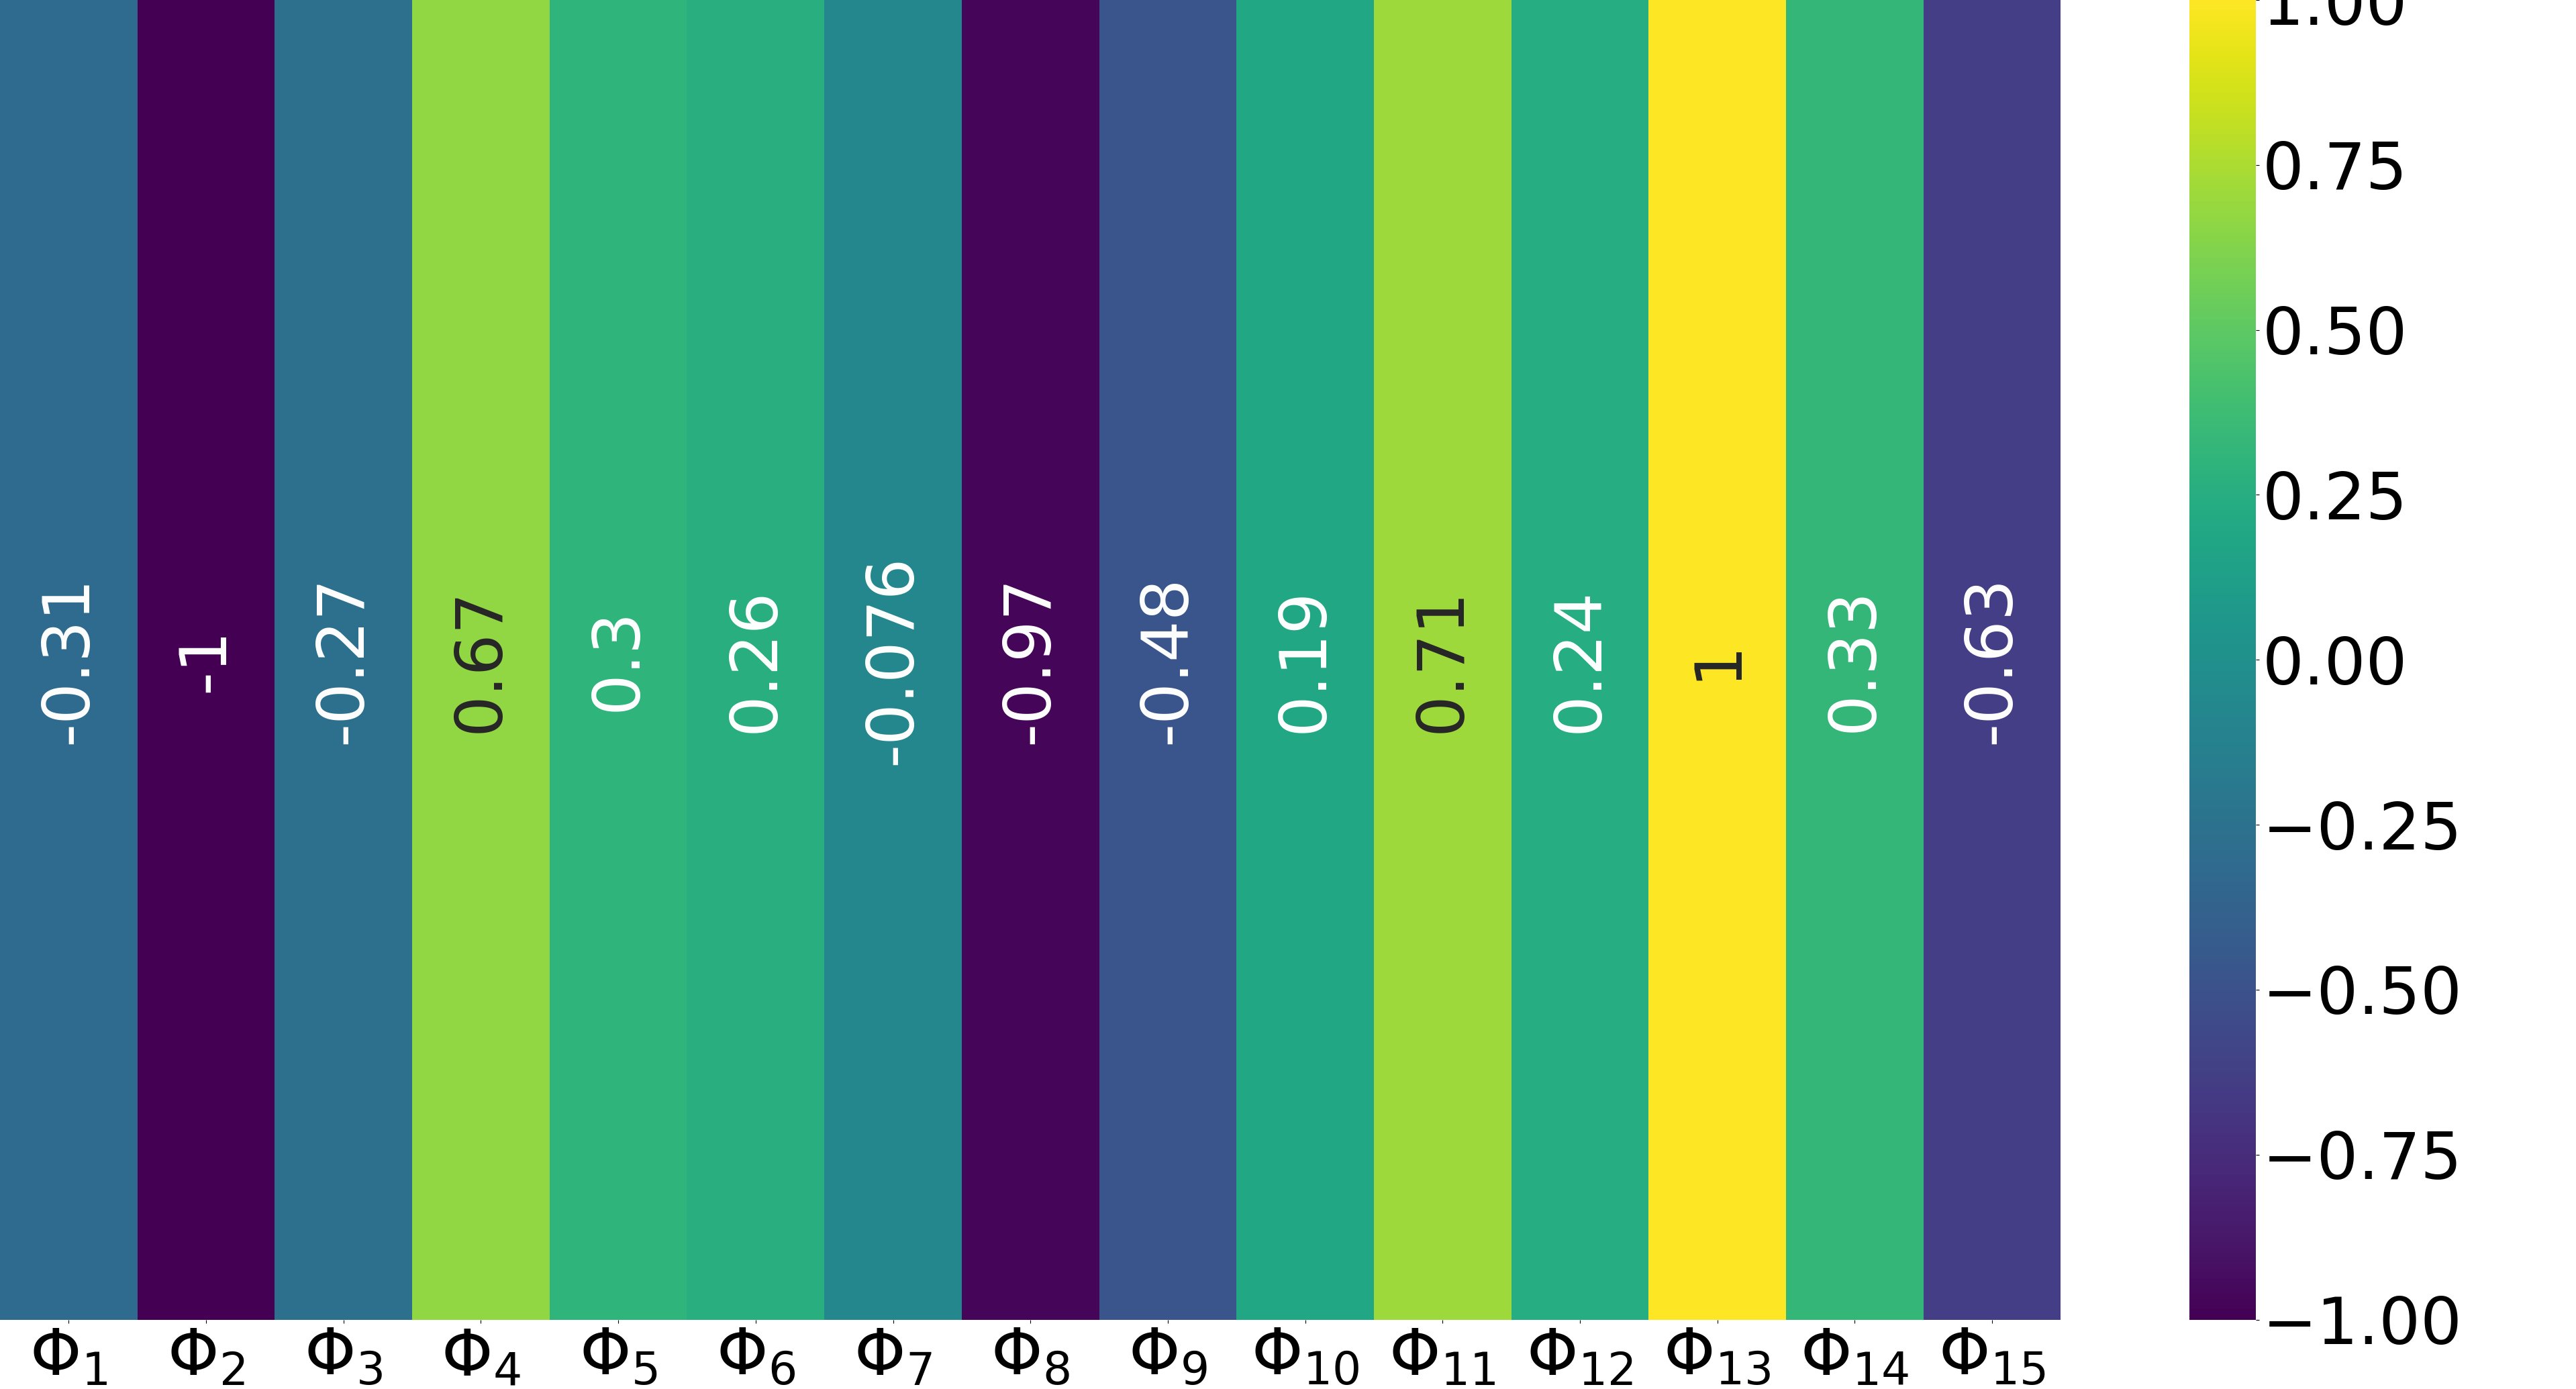
\includegraphics[width=\linewidth]{img/qlp_corr/Phi_coil3.png}
		\subcaption{Correlation with coil $3$}
	\end{subfigure}
	\caption{Correlation between the harmonics of the \phin\ attribute and the labels for \qlp.}
	\label{fig:phi-lcorr-qlp}
\end{figure}

\begin{figure}[!ht]
	% Font size = 40
	\centering
	\begin{subfigure}{0.8\linewidth}
		\centering
		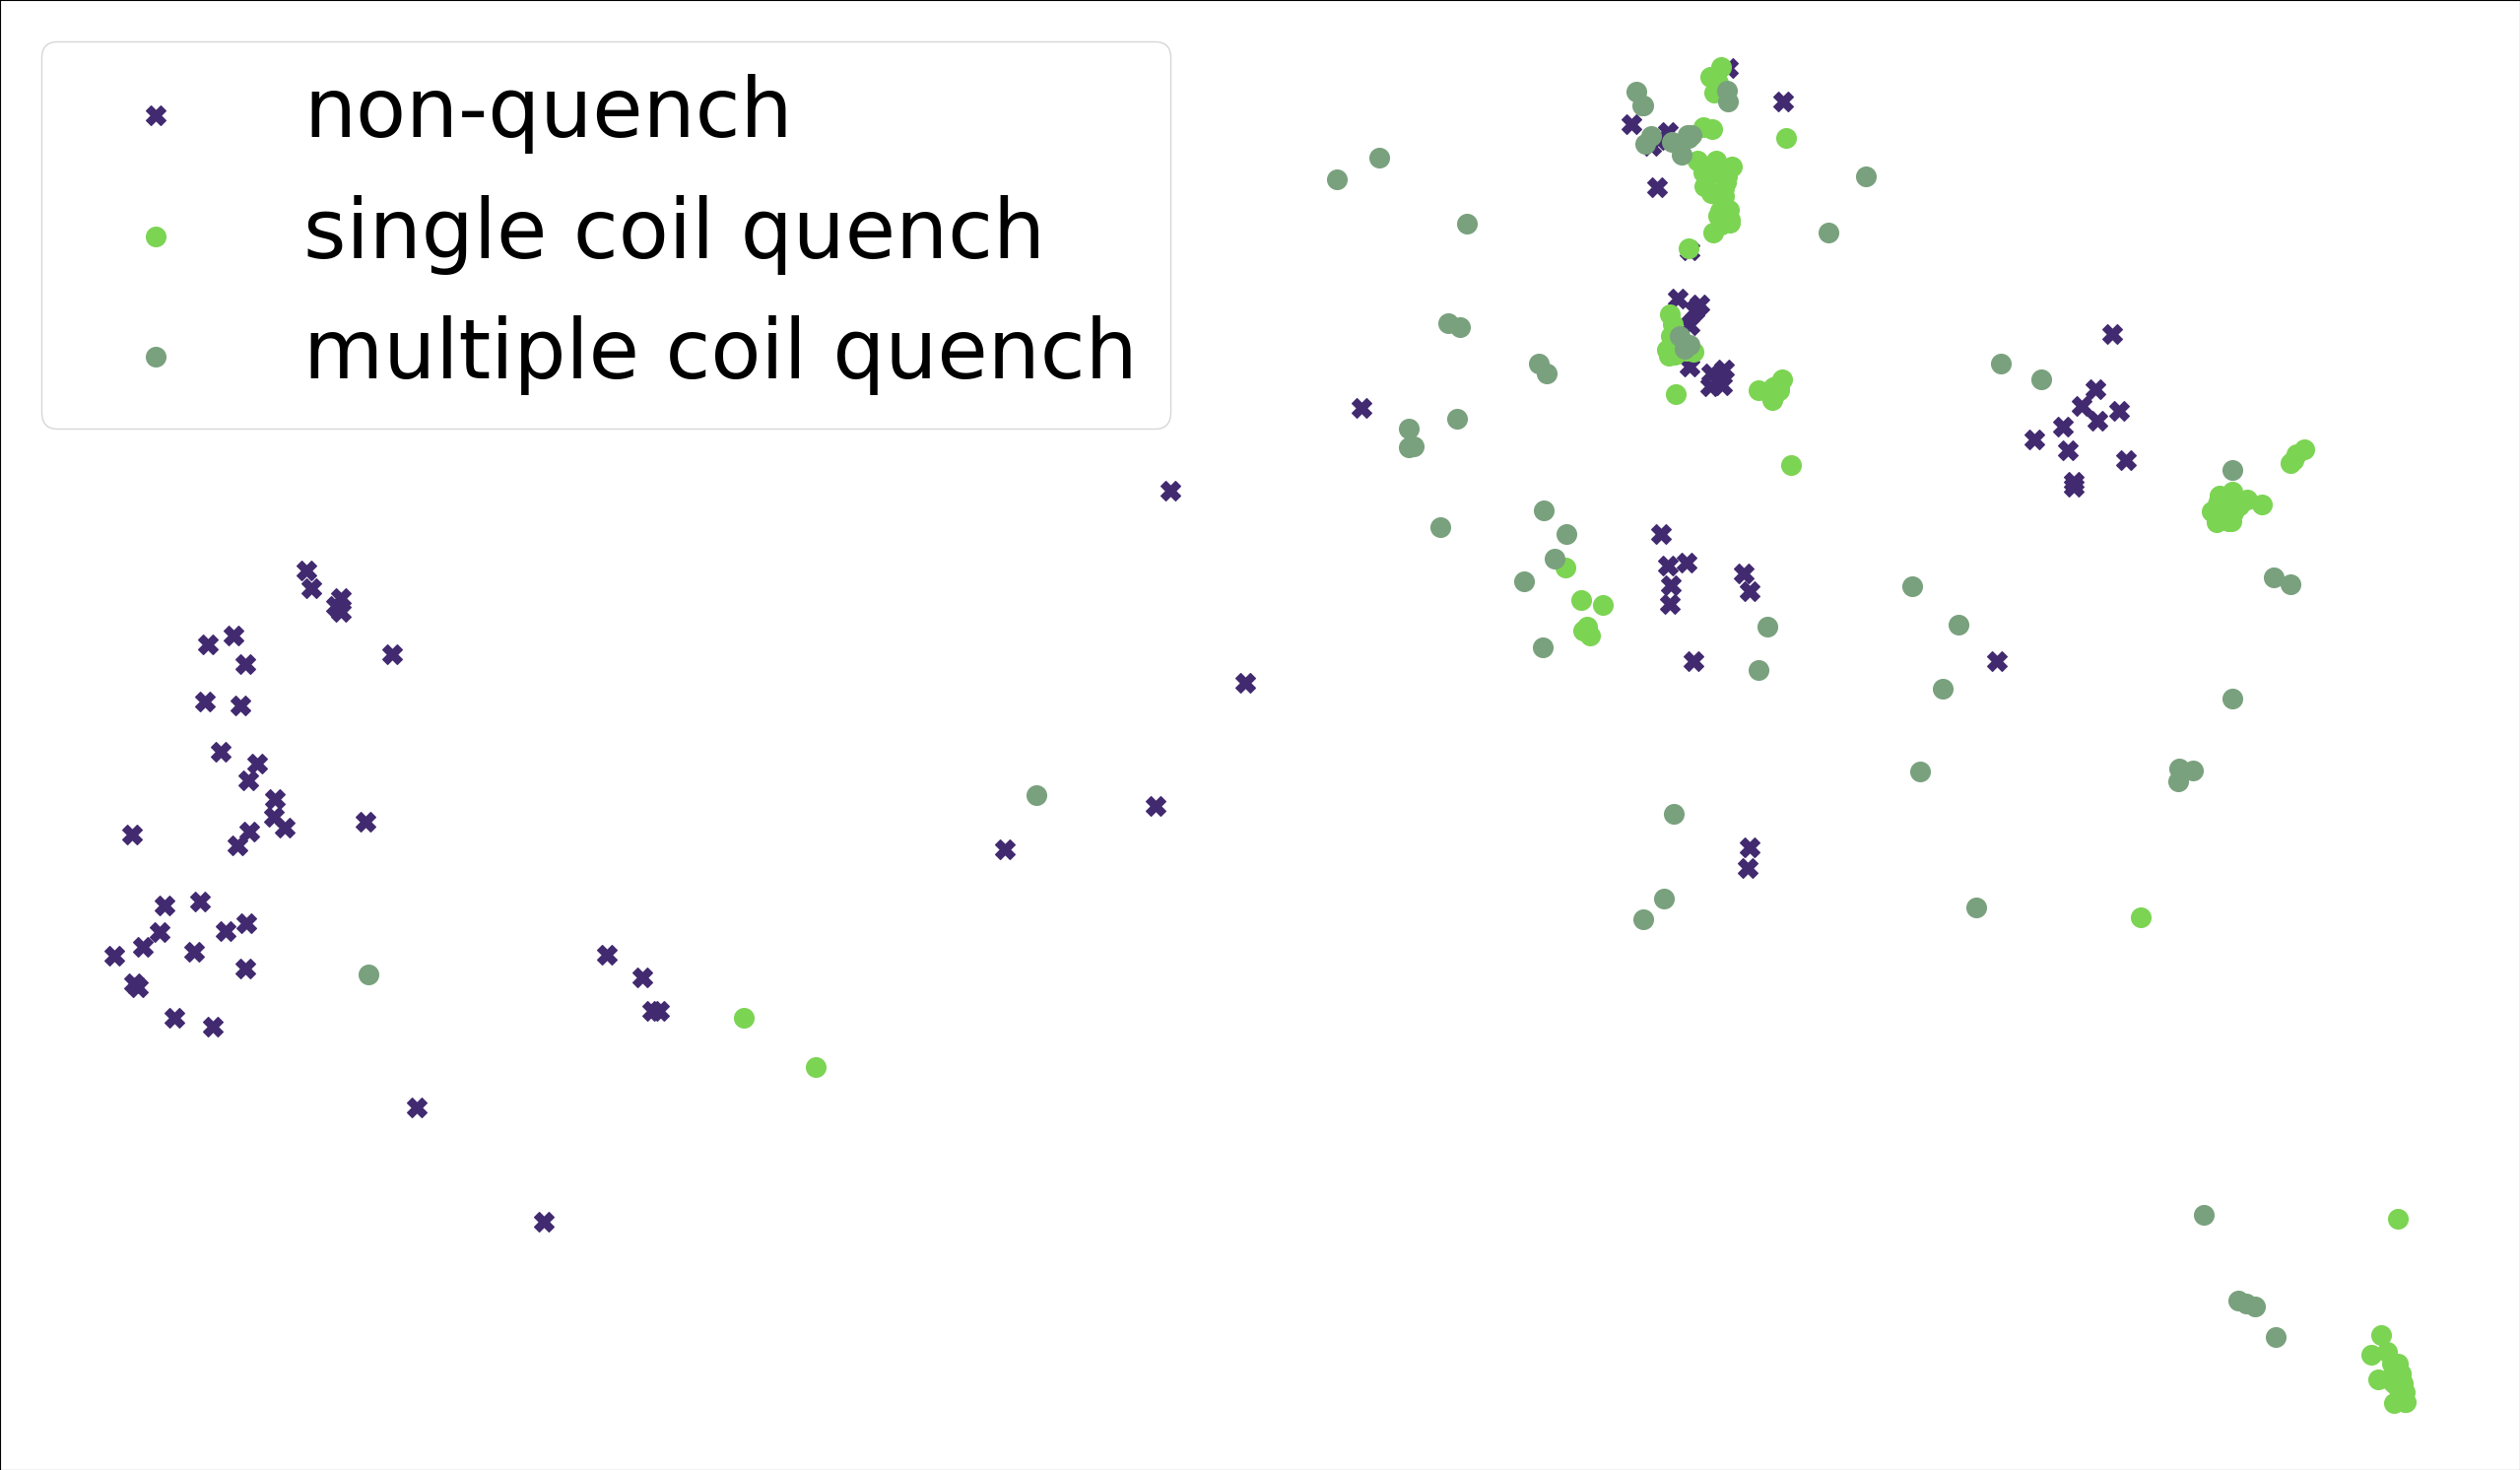
\includegraphics[width=\linewidth]{img/quench_dist_qlp/single_vs_multiple_Phi.png}
		\subcaption{}
	\end{subfigure}
	\begin{subfigure}{0.8\linewidth}
		\centering
		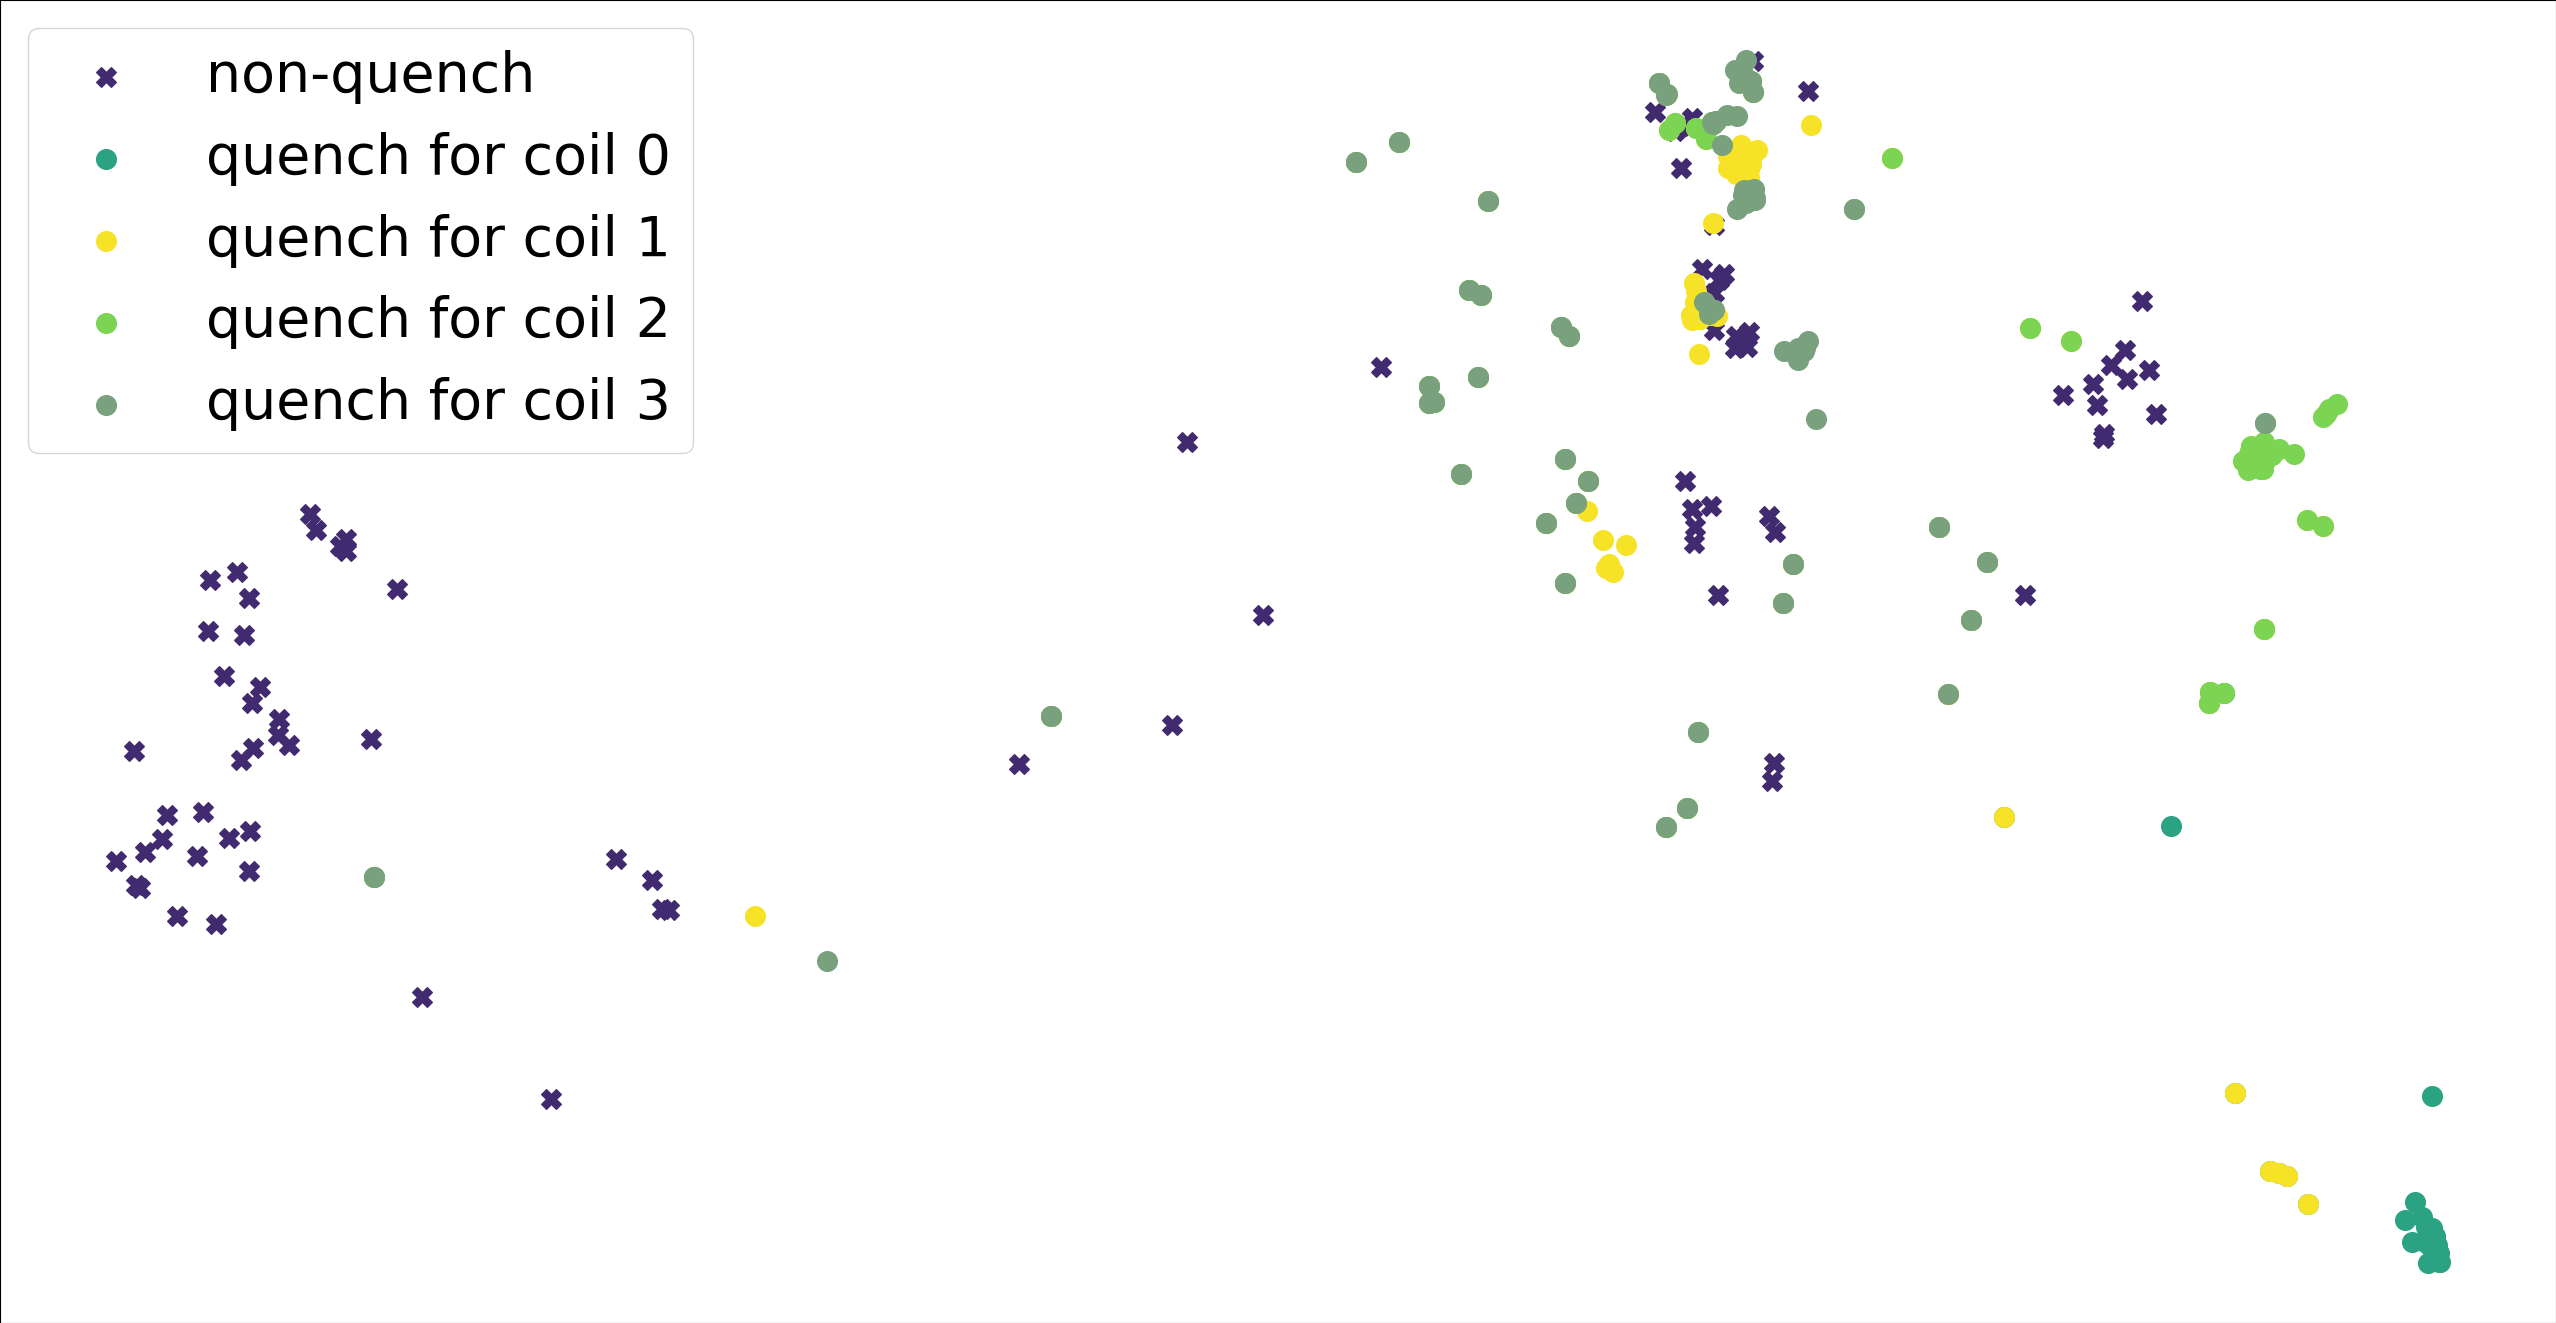
\includegraphics[width=\linewidth]{img/quench_dist_qlp_phi.png}
		\subcaption{}
	\end{subfigure}
	\caption{Visualization of the \phin\ attribute, the data was plotted after a run of \pca\
		dimensionality reduction. Sub-figure (a) highlights the samples based on how many quenches
		are associated to the specific sample $\{0, 1, \text{many}\}$. Sub-figure (b) highlights the
		samples based on the specific coil quenched $\{\text{None}, 0, 1, 2, 3\}$.}
	\label{fig:phi-coilq-dist}
\end{figure}

\section{First approaches using Clustering}
\label{sec:qlp-cluster}
We initially discovered that \an\ and \cnmod\ data was scattered favorably in bidimensional space
while we were still studying \qrp. We decided to use clustering because it was unsupervised,
and we wanted to understand if there was a way for us to get very early results in \qlp\ by
leveraging some undiscovered patterns in the data.

We remark that the clustering algorithm is always working by using distance between samples,
therefore the pattern that it's capable of identifying is unknown to us, and we, as researchers,
have to identify it. Even if we applied clustering to all the attributes, we will only show
relevant results obtained on \an\ and \cnmod. Data was plotted using \pca, but we also explored
other dimensionality reduction techniques, namely FastICA and Metric multiDimensional Scaling (MDS),
generally yielding inferior results.

\Cref{fig:4-means-results} shows results of a $4$-means clustering run on both attributes, we chose
to label the samples based on the number of quenched coils $\{0, 1, \text{many}\}$. The orange lines
in the figure represent the cluster borders, if the line is solid then the cluster has a finite size, otherwise the cluster has infinite size.

While the result for \an\ (sub-figure (a)) contains $3$ clusters that essentially have a high degree
of purity (the top for the magnet in normal operating conditions, the left and right for quench
events). The central cluster mixes quench and non-quench data, making it less useful for our
classification needs. If we consider \cnmod (sub-figure (b)), while it's far from perfect, we can see
that the clusters have a decent level of purity.
\begin{figure}[!ht]
	\centering
	\begin{subfigure}{0.8\linewidth}
		\centering
		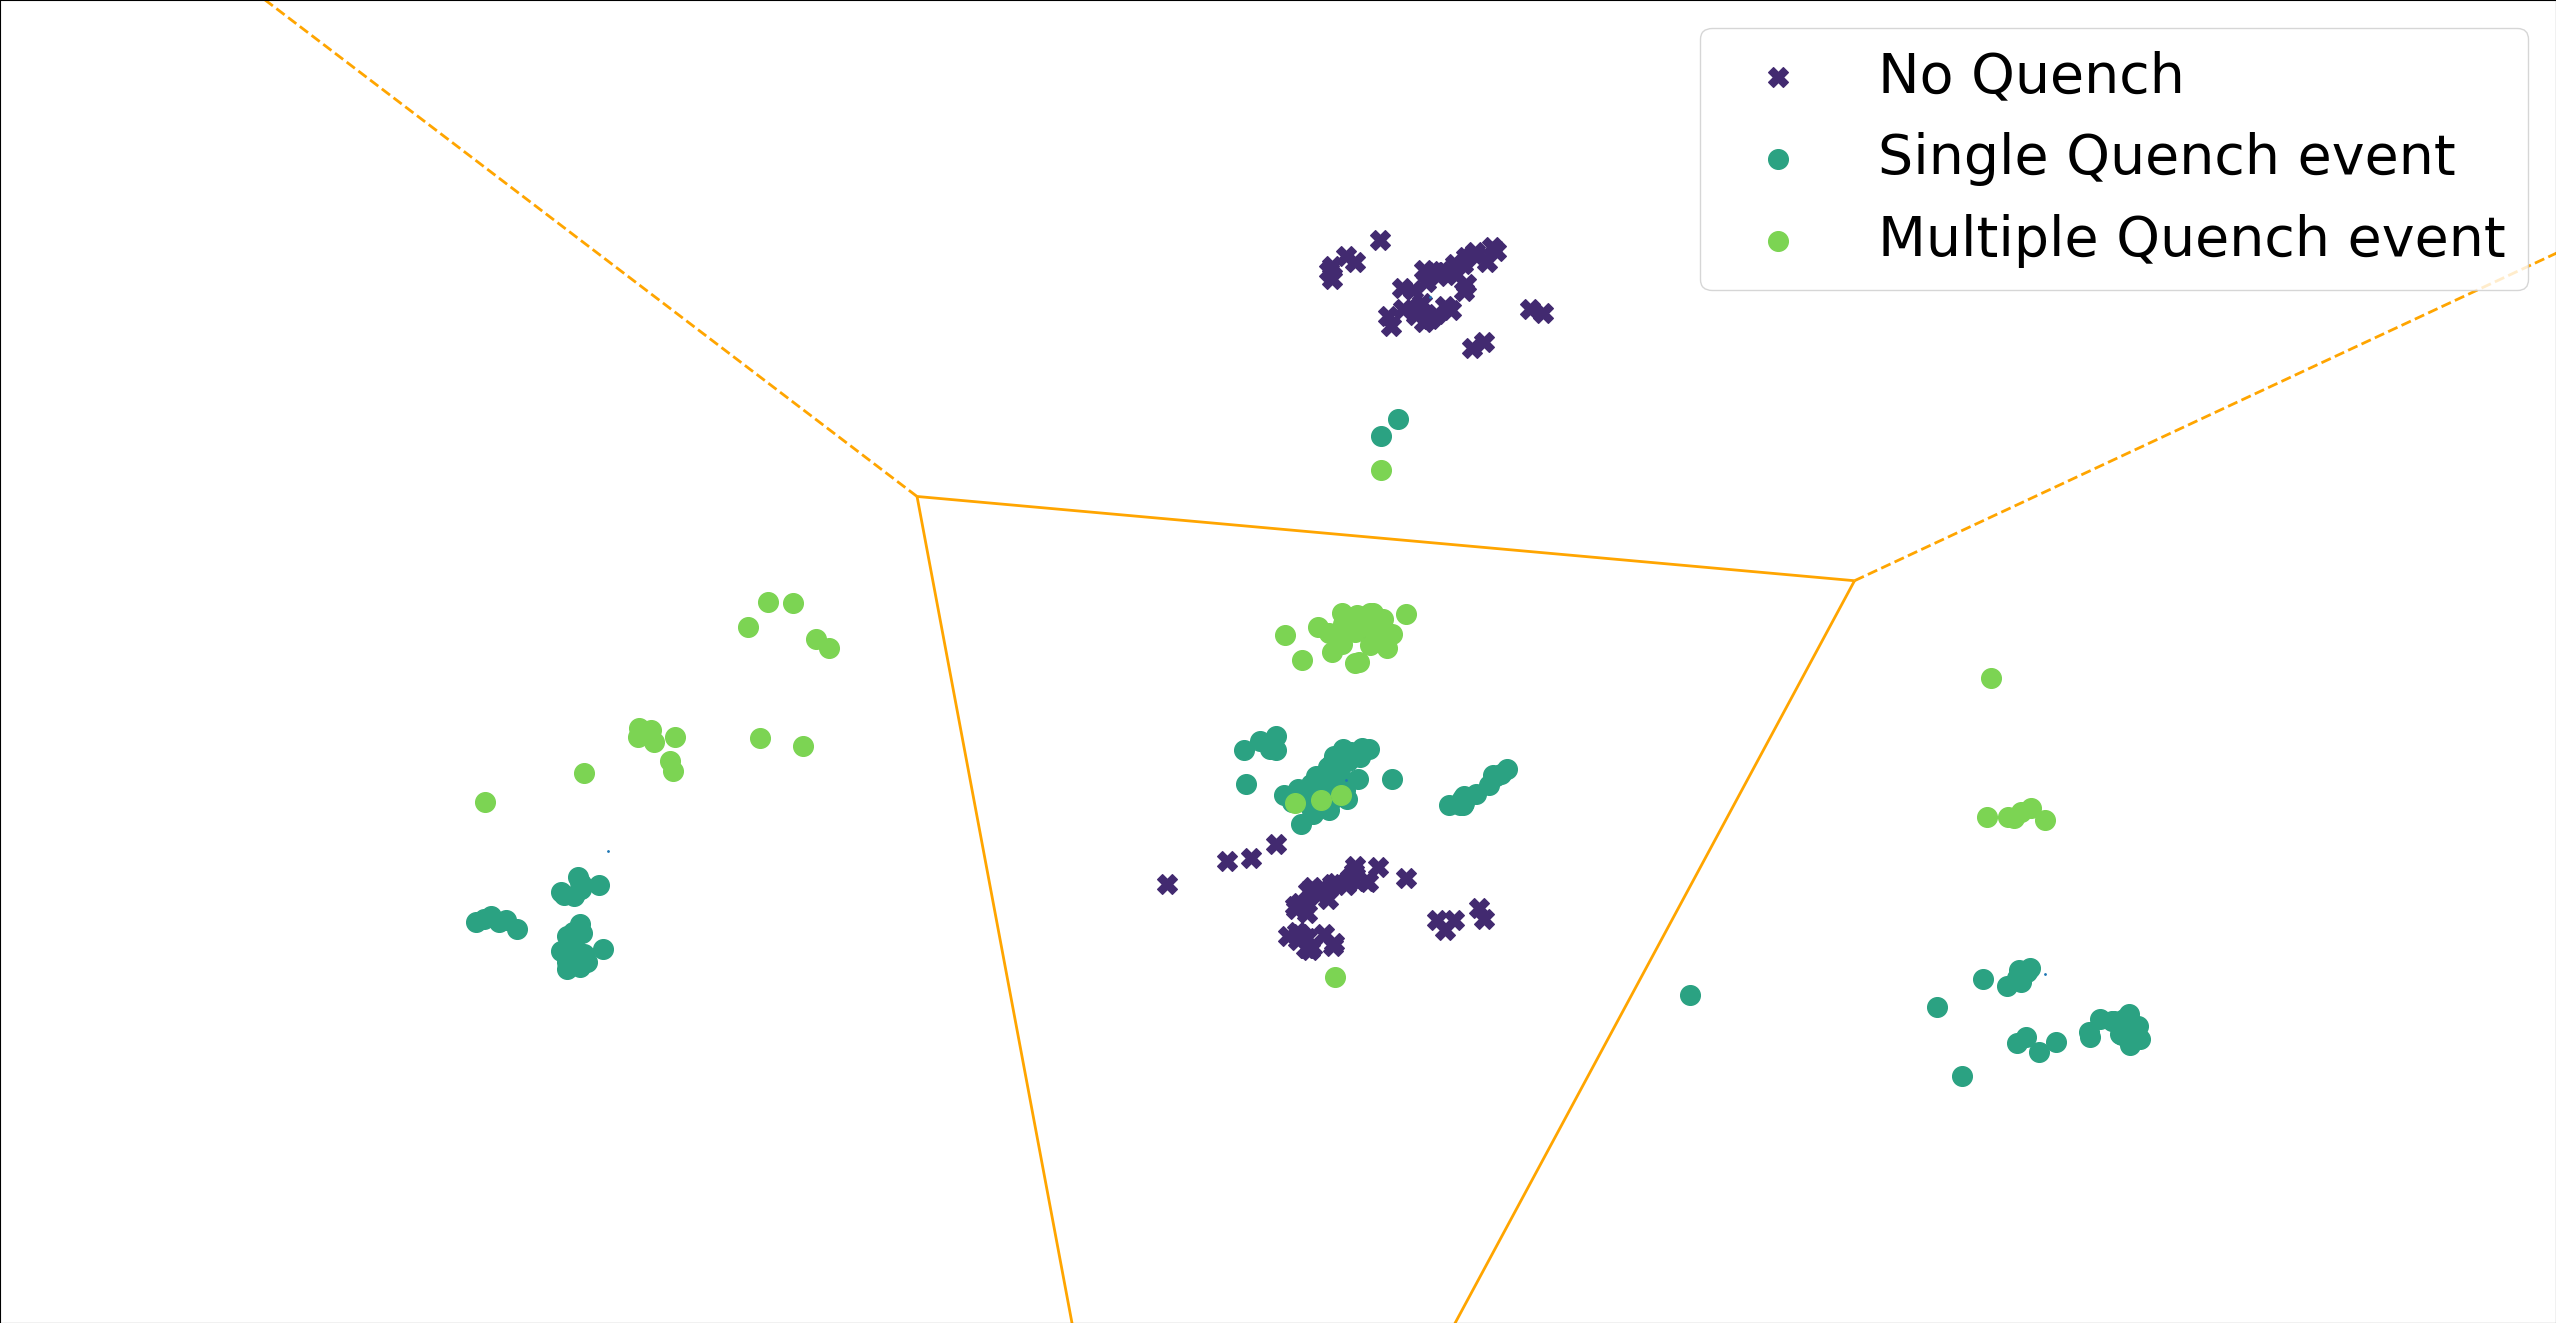
\includegraphics[width=\linewidth]{img/clustering_an_qlp_4c.png}
		\caption{}
	\end{subfigure}
	\begin{subfigure}{0.8\linewidth}
		\centering
		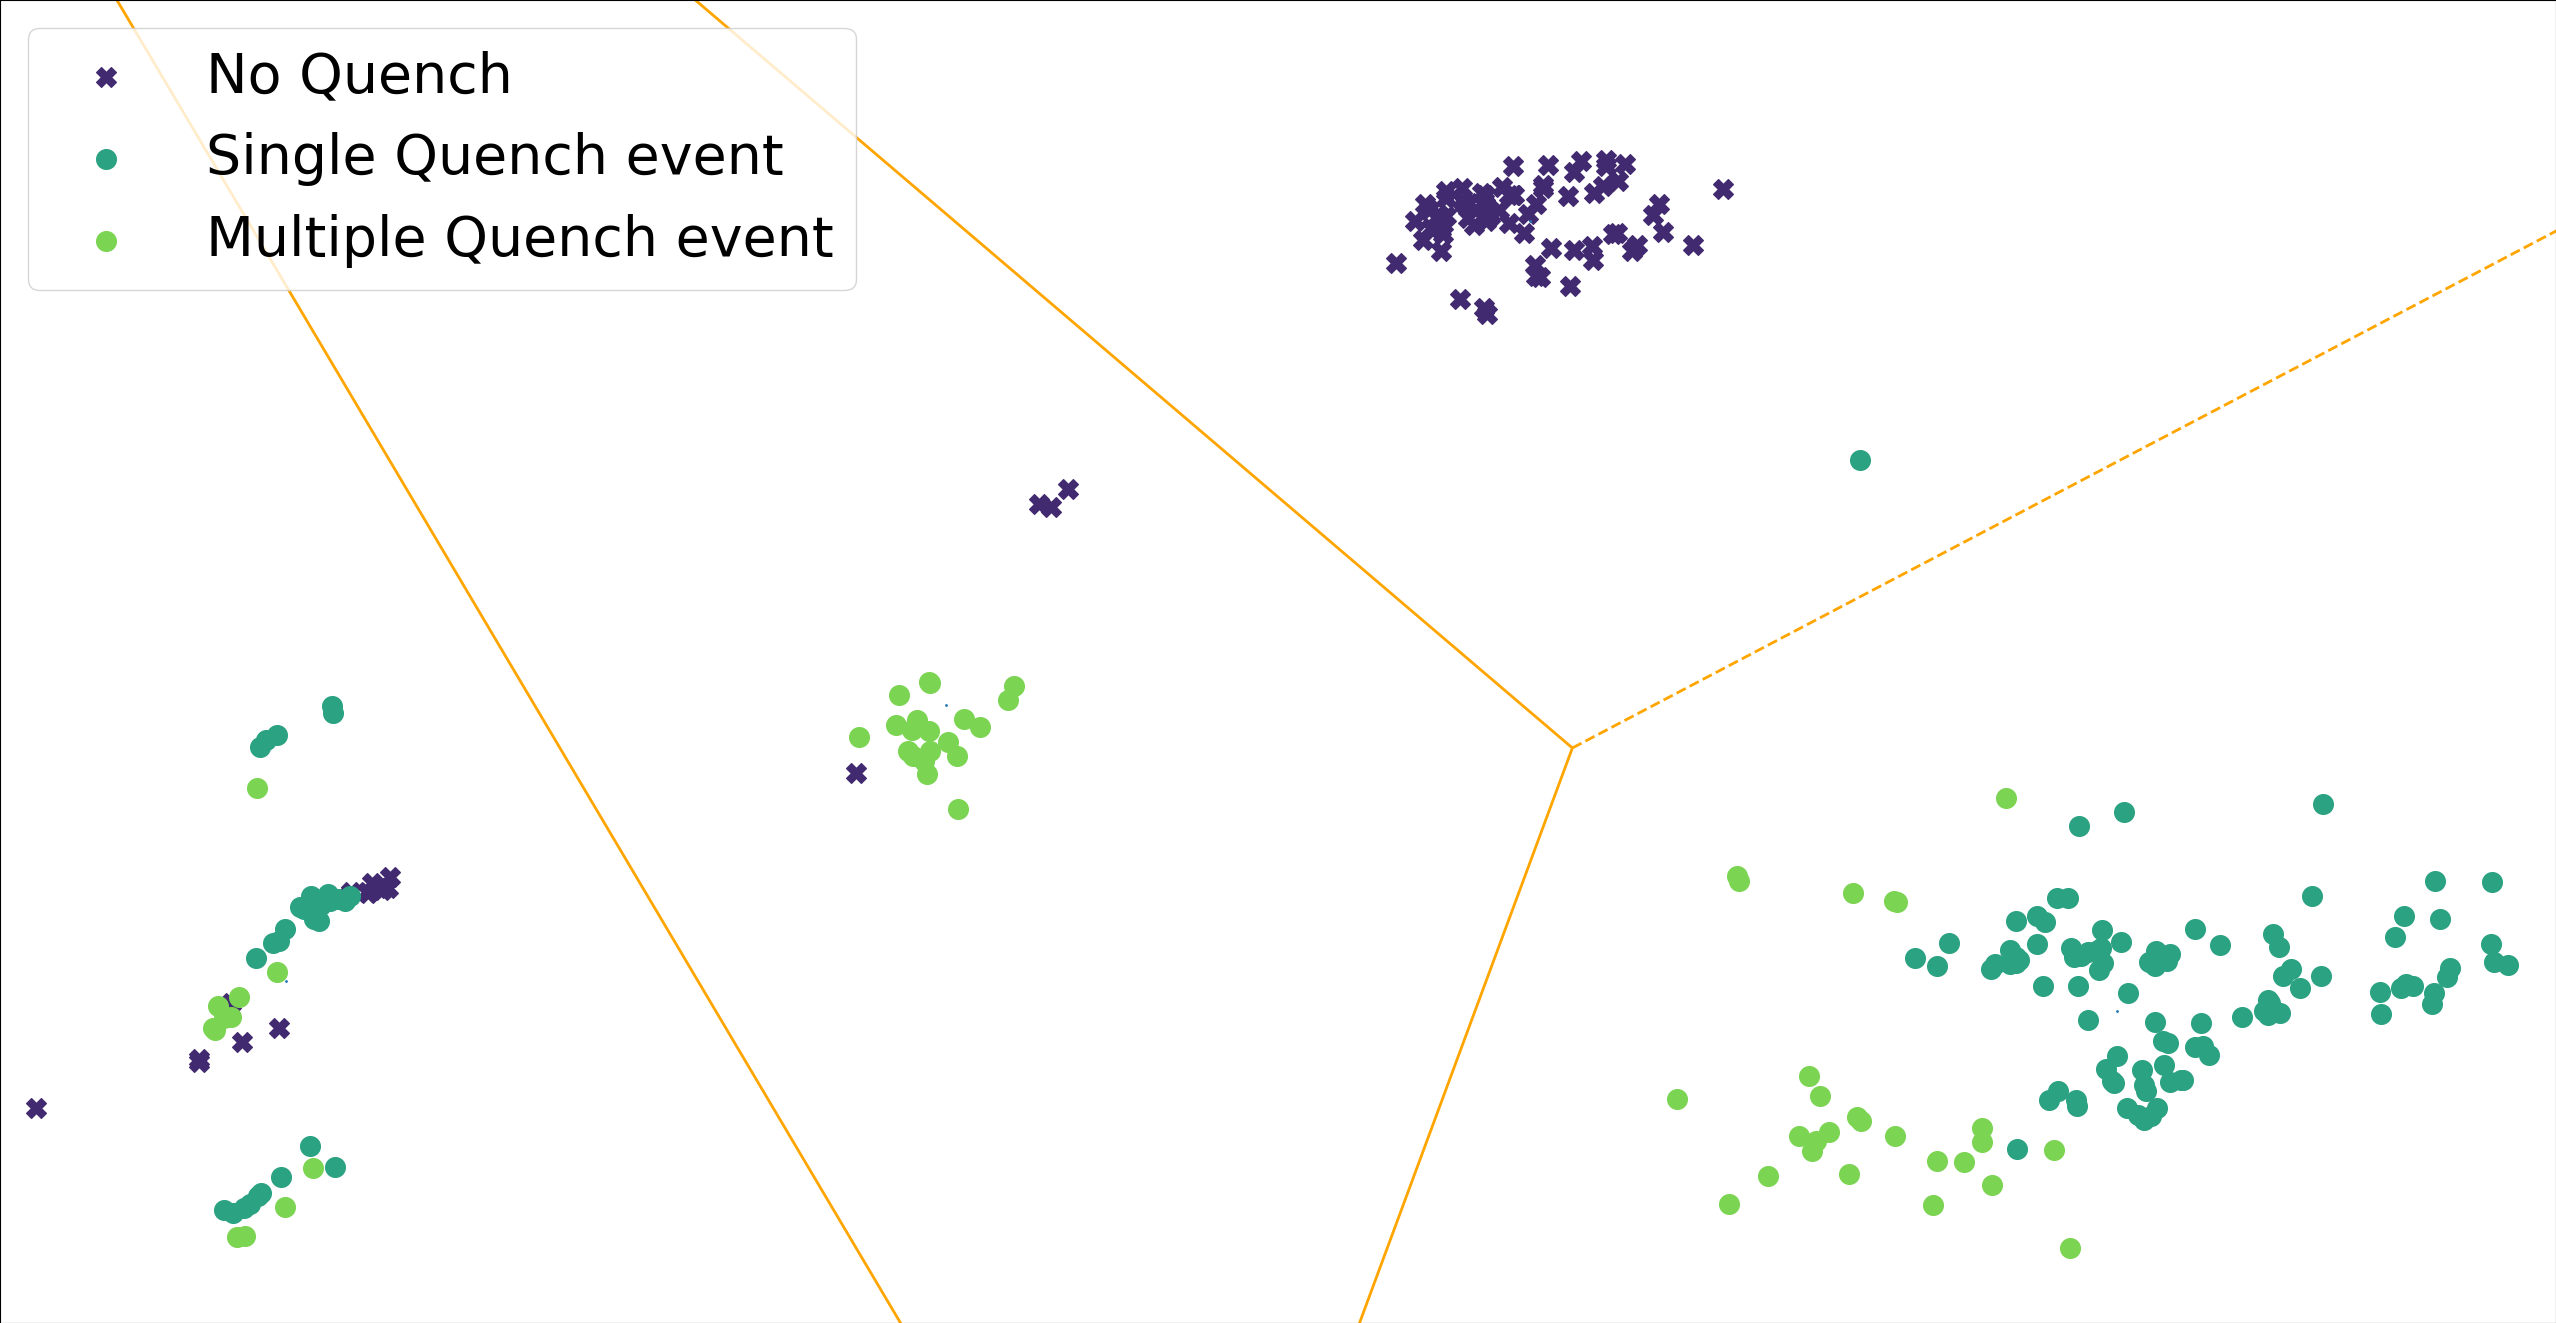
\includegraphics[width=\linewidth]{img/clustering_cnmod_qlp_4c.png}
		\caption{}
	\end{subfigure}
	\caption{A run of $4$-means on attributes \an\ and \cnmod\ after a round of \pca\
		dimensionality reduction. As we can see using $4$ clusters leads to a suboptimal division of
		the samples, while \cnmod\ has clusters with a bit more purity (at least quench-events are
		not mixed with non-quenches).} \label{fig:4-means-results}
\end{figure}

According to the clustering-specific performance metrics (Silhouette and \textsc{db} scores, cfr.
\Cref{chp:ml}) for both \an\ and \cnmod, using $4$ clusters represented the best possible solution.
As we discussed above, though, this choice lead to suboptimal results, especially for \an.  We
experimented with higher cluster counts, and discovered that, while the result gets visually worse
for \cnmod, probably because it's trying to split single quench clusters belonging to different
coils (cfr. the south-east sector in \Cref{fig:cnmod-coilq-dist}, sub-figure (b)). A run of
$8$-means on \an\ generates clusters with a high level of purity. \Cref{fig:clustering-an} plots the result, the clusters identified by the algorithm are very clearly trying to separate three classes of samples: one associated to the magnet being in normal working condition, one associated to the magnet containing \emph{at most} one quenched coil, and finally, one associated to the magnet containing \emph{at least} one quenched coil.
\begin{figure}[!ht]
	\centering
	\includegraphics[width=0.8\linewidth]{img/clustering_an_qlp_8c.png}
	\caption{The results of a run of $8$-means on the sole attribute \an, after a round of \pca
		dimensionality reduction. As we can see all clusters have a high purity and only a handful of points have been misclassified.}\label{fig:clustering-an}
\end{figure}

Using clustering we achieved very interesting results and, while it's not a technique that can be
used as a classifier on its own (not even in cases in which the performance seems to be the best),
we could easily use it as a preprocessing step for other models like decision trees, or for a run of
the supervised clustering algorithm $k$-nn.

\section{Results}
After our brief exploration of the possibilities offered by clustering algorithms, we moved back to
supervised machine learning algorithms to solve \qlp. Our first approach was to do a na\"ive
extention of the models used to solve \qrp, to the multiclass-classification environment. We didn't
have high expectations for such models since they would have to predict $4$ different bits, instead of just one, making the problem
much more difficult than the original one.

As a matter of fact, trees, which have always been quite easy to interpret, in the case of \qlp\
became much more complicated to read. Even if they always had maximum depth between $5$ and $10$
(therefore having a structure close to the limit of what we would consider explainable) the accuracy
was close to $60 - 70\%$. This rough performance number was obtained by micro averaging the accuracy
for every class, in other words, the resulting metric is the average of the metric computed on each
class weighted on the cardinality of the class.

Since the performance obtained using a direct extension of trees didn't really suit our expectations
we chose to change approach. Our new idea was simply to turn \qlp\ into a problem that could be
solved by simply solving a variation of \qrp\ $4$ different times, one per coil. We solved a
variation of \qrp\ and not \emph{the actual} \qrp, since the relation we originally wanted to find
connected the harmonic decomposition of magnetic field to quench events in a quadrupole. This new
version of \qrp\ requires us to find a function that links \emph{the same data} to a different
value, that states whether coil $i$ quenched or not.

It might sound like a very subtle change, but it's an important one. So much so that, if we tried to
reuse the best models we found for \qrp, to solve \qlp, we wouldn't get similar performance metric.
In the following sections we will retrace our steps in \Cref{chp:qrp} and discuss the obtained
results for the various models.

\subsection{Decision trees}
As we said previously, decision trees utilized in the multiclass-classification environment provided
performance that left a lot to be desired, to counteract this we chose to reinterpret \qlp\ as a
problem in which we need to understand whether each coil has quenched, separately (therefore
solving \qrp\ $4$ different times). To keep the discussion of the performance concise we will be
discussing the structure of the best models and concentrate on the performance of the aggregate.

To evaluate the performance of the aggregate model, containing one classifier per coil, we defined a
metric named 'Hamming score' ($\hs$ in the following), which simply computes how different are the
prediction and the expected outcome.

\Cref{fig:bdts-qlp} contains the performance metrics obtained in the outer \cv\ for the best single
tree trained on each coil. The metrics are quite close to each other, with the only clear outlier
being the model trained on coil $3$.

Instead of including a plot of the various trees we condensed the most important information
in \Cref{tbl:tree-description}, all the trees described have a depth of maximum $5$ and the number
of internal nodes and leaves is always very acceptable, while the trees built on \an\ remain on the
smaller side, the trees built for coil $1$ and $3$ are larger (with the one built on \cnmod\ being
the largest at $15$ total nodes), despite their structure being more complex, these trees struggle
compared to the ones trained on sub-views of \an.

\begin{figure}[!ht]
	\centering
	\includegraphics[width=\linewidth]{img/best_dts_qlp.png}
	\caption{Comparing the performance of the best model built on every coil, independently of
		the dataset used.} \label{fig:bdts-qlp}
\end{figure}

\begin{table}[!ht]
	\caption{Description of the best \dt\ for every coil.}\label{tbl:tree-description}

	\bigskip
	\setlength{\tabcolsep}{6pt}
	\centering
	\begin{tabular}{lcccc}
		\toprule
		\textbf{}                           & \textbf{Coil 0}  & \textbf{Coil 1}          & \textbf{Coil 2}          & \textbf{Coil 3}
		\\
		\midrule
		\textsc{attribute}                  & \an              & \bn                      & \an                      & \cnmod                          \\
		\multirow{2}{*}{\textsc{harmonics}} & \an[2], \an[3]   & \bn[3], \bn[4], \bn[10], & \an[1], \an[2], \an[12], & \cnmod[1], \cnmod[6], \cnmod[7] \\
		                                    &
		                                    & \bn[11], \bn[13] & \an[15]                  &                                                            \\
		\textsc{depth}                      & 3                & 5
		                                    & 3                & 5                                                                                     \\
		\textsc{N internal nodes}           & 4                & 5
		                                    & 3                & 8                                                                                     \\
		\textsc{N leaves}                   & 5                & 6
		                                    & 4                & 7                                                                                     \\
		\textsc{N nodes}                    & 9                & 11
		                                    & 7                & 15                                                                                    \\
		\bottomrule
	\end{tabular}
\end{table}

In \Cref{fig:dt-qlp-hs}, we plotted the performance of the aggregate model, which are obtained as we
did when testing \tas\ for \qrp: A run of $5$-fold \cv\ and we computed the number of errors done by
the ensemble on the $4$ bit array. On average the classifiers makes $2$ errors or less, since the
minimum accuracy is $0.5$, averaging the performance of all the folds we get a final Hamming score
which is $0.95$ and with a standard deviation of $0.024$. Testing the performance of the aggregate
on the final blind-test, if we average the Hamming score on the $29$ samples, we get higher
performance on average $0.966$ and a higher standard deviation $0.086$ (this difference is probably
due to the lower amount of data we are averaging on), the trained aggregate makes $4$ single errors
on the $116$ total labels that it needs to predict.

Our supposition at the moment is that finding a better model for coil $3$ would make the performance of
the ensemble better because, while we have been saying that the model is an aggregate of trees, no
aggregation is happening (like in the case of \tas) apart from inserting the predicted bits in a
prediction array, therefore the sub-models are not helping each other and 'covering for each other'.

\begin{figure}[!ht]
	\centering
	\includegraphics[width=\linewidth]{img/best_dts_hs.png}
	\caption{The Hamming score computed on every fold (for the $50$ samples therein contained), the lower reaching is the line the lower is going to be the accuracy.} \label{fig:dt-qlp-hs}
\end{figure}

\subsection{Random forests}
Similarly to what we just did for \dts\ we also evaluated the performance of a model containing one
single forest per coil, we expected higher performance compared to the ones just obtained on \dts,
at the expense of a lower explainability.

\Cref{fig:brfs-qlp} shows the performance for the best rfs built on a mix of different attributes
(each taken in its entirety), as we can see the performance metrics are better, but we are not far
off from the numbers obtained in the case of \dts\ (see \Cref{fig:bdts-qlp}), also, our weakest
learner, the one built for coil $3$ is not much worse than the proposed random forest, while being
much simpler than the alternative.
\begin{figure}
	\centering
	\includegraphics[width=\linewidth]{img/best_rfs_qlp.png}
	\caption{The best random forest trained on a sub-view or mix of sub-views, for every coil,
		since all of the models have been plotted without indicating the harmonic content it means
		that they are using full attributes.}\label{fig:brfs-qlp}
\end{figure}
The \rfs\ in figure contain respectively $5, 10, 10$ and $10$ trees. As we have already said
previously, while trees have a high level of explainablilty, trying to interpret a structure
containing $10$ of them is certaintly a complex task, and I would consider it explainable only on
paper. This is why, for all intents and pourposes, while we provide the results for the Hamming
score in the following, we decided to not follow this lead too much, since it would mean having an
excessive amount of models to consider at the same time.

While the trees for the first three forests are, overall, quite simple (not too deep), contained in
the number of leaves and nodes, the last forest contains complex trees with many layers ($4$ on
average), many internal nodes and leaves. Seeing the complexity of this last tree it's evident that
the forest approach would not be feasible even in an hybrid approach based on both three trees for
the first three coils and an \rf\ for the last one.

Since \rfs\ are more complicated than we would like we avoided the calculation of the Hamming
score, also because the performance are good but not good enough to make us consider their use when
compared to the simpler \dts.

\subsubsection{Support Vector Classifiers}
If we analyze the benchmark model, and we train it without constraints (one or more sub-views for
different datasets), the results are that we can aim at a very high level of performance if we
forget about explainability. Performance have been plotted in \Cref{fig:bsvcs-qlp}, the metrics were
taken from the outer \cv\ loop and the models chosen were the best for each specific coil.
\begin{figure}[!ht]
	\centering
	\includegraphics[width=\textwidth]{img/best_svcs_qlp.png}
	\caption{Performance metrics for the best \svcs\ trained on every coil, all attributes
		have been taken with their full harmonic content.} \label{fig:bsvcs-qlp}
\end{figure}
There are a couple of very interesting takeaways:
\begin{itemize}
	\item The best \svc\ trained on coil $0$ is based on attribute \an. This is exactly what we
	      expected since the very beginning of this chapter.
	\item The best models for coils $1$ and $3$, were trained on \bn\ and another dataset (\cnmod\ for $1$
	      and \phin\ for $3$). This is interesting for two reasons:
	      \begin{inparaenum}[(i)]
		      \item \bn\ is actually the best attribute for the two coils, as we saw in the analysis
		      we did in the beginning of the chapter,
		      \item the \svc\ trained on the sole \bn\ performed worse than the alternatives. This
		      lead us to believe that, like in the case of \qrp, \bn\ alone doesn't contain
		      enough information
	      \end{inparaenum}.
	\item Interestingly, while \cnmod\ didn't perform well enough in our tests on trees for coil
	      $2$, in the case of \svc\ the model was picked over \an.
\end{itemize}
Evidently, the ceiling of performance is still very high, and we can still find ways to get closer
to the performance of our benchmark model.









\chapter{Conclusions}
\label{chp:conclusion}
In this thesis we have proposed a solution to the problem of identifying quench events and
localizing them within the magnet structure using the harmonic decomposition of magnetic field. We
have provided a very strong solution for the first, and we have provided a good starting point for
the second. During the project, we had different ideas to branch out and further explore the
fascinating realm of machine learning applied to superconductor physics.

We remark that, while the analysis we have done has been thorough, the performance achieved and the
identified models only work on the specific case of the High order corrector quadrupolar magnets.
We have serious doubts that this analysis could be extended to any other quadrupole; and extending it to magnets with a different number of poles would yield unusable results.

To achieve higher performance on \dts\ for \qlp, we can do further analysis on the models we
identified so far; or we can opt for a more powerful model and opt for \emph{post-hoc}
explainability~\cite{retzlaff2024}. While in the first case it's only a matter of experimentation,
in the second case we would need more data, but the result of such an analysis wouldn't necessarily
yield highly explainable results.

\subsubsection{Analysis of the decision rules and general detection model}
In the project we have identified highly explainable models, capable of solving \qrp\ and \qlp\
maintaining high performance. The obvious next step, is to open the models and abstract
useful rules, capable of explaining quench and localizing events in certain coils. These rules could
be used:
\begin{itemize}
	\item In the field of sensor calibration, to isolate the harmonics that we truly need; simplifying sensor design, while also making the Quench Protection System more efficient,
	\item Support in the magnet design process.
\end{itemize}

\subsubsection{Fuzzification of quench-event description}
For both our problems the quench-event was described by a binary value, if $0$ then the sample
remained in the superconducting state, if $1$, then the material transitioned to the
normal-conducting state. An interesting option would be to change the description of quenches,
moving to a representation of the label as a real number in the interval $[0, 1]$.

By moving to this new description we could leverage a higher expressivity, highlighting different
behaviors: characterizing the rapidity of a transition to the normal-conducting state, or measuring
the violence of the quench transition (how high is the spike of resistive voltage for the quench
precursor). The ones above are just examples, we could use this new labelling system do explain
different aspects of the magnet. The different descriptions would have to be inspected by a
Physicist to understand which correlation is more interesting to investigate.

\subsubsection{Analysis of Voltage data}
In the original experiment two different measures were taken on the magnets: magnetic measures (the
ones we used throughout this thesis) and voltage taps. Voltage taps are used to measure the voltage
in different positions inside the magnet, these taps are then connected to the electronics of the
\textsc{qps}.

The magnetic measurement system is much slower compared to the voltage measurement system; this
means that we have much more data at our disposal that has not yet been used. At the time of writing
we are starting a cooperation with Naples University to build high-performance models on such data.

\subsubsection{High performance quench localization}
High-performance models for online quench detection and localization, are a different area of
research (quite active at the moment~\cite{hoang2021, zhou2021, einstein2023}).

Many are the alternatives: the \svcs\ explored in this thesis, neural networks or anomaly detection
via autoencoders. Clearly, pursuing such path forces us to invalid the explainability property we
granted throughout the project, unless explainable-ai models were used.

\subsubsection{Clustering-based preprocessing for classification}
Another technique that could be worth exploring is Clustering. We saw in the last chapter how the
points were very nicely distributed in bidimensional space, specifically for attribute \an, but also
for attribute \cnmod.

As we said in \Cref{sec:qlp-cluster} we could likely use clustering as a preprocessing step and then
extrapolate the results using highly explainable models like \dts\ and \rfs. We could also do a
first run of $k$-means clustering and then finalize classification using $k$-nn. Both approaches
would be extremely viable, at the expense, once more, of explainability (since we use $k$-means and
\pca, which are inherently non-explainable).






\part*{Appendix}
\appendix
\chapter{Karush-Kuhn-Tucker conditions}
\label{app:kkt}
Equation~\ref{eq:opt-problem} defines a non-linear optimization problem, we consider a minimization
problem, with both inequality and equality constraints. Karush-Kuhn-Tucker conditions (\kkt) are
necessary conditions to solve such problems.
\begin{equation}
	\label{eq:opt-problem}
	\begin{aligned}
		\min{f(x)} &        \\
		g_i(x)     & \leq 0 \\
		h_j(x)     & = 0
	\end{aligned}
\end{equation}

To make sure that \kkt\ can identify local minima it's important that the regularity condition for
constraints is satisfied. One of the following conditions needs to be valid for $x^*$ to be a local
minimum for the objective function:
\begin{enumerate}
	\item Linearity constraint qualification (\textsc{lcq}): if $g_i$ and $h_j$ are affine functions, then no
	      other condition is needed.
	\item Linear independence constraint qualification (\textsc{licq}): The gradients of the active inequality
	      constraints and the gradients of the equality constraints are linearly independent at $x^*$.
	\item Constant rank constraint qualification (\textsc{crcq}): For each subset of the gradients of the active
	      inequality constraints and the gradients of the equality constraints the rank at a vicinity
	      of $x^*$ is constant.
\end{enumerate}
This is only a small selection of the available conditions, the lower the rank, the broader the
applicability ($\textsc{lcq} \implies \textsc{licq} \implies \textsc{crcq}$).

If $x^*$ is a point that satisfies the regularity conditions just introduced, $f: \R^n \rightarrow
	\R$, $g_i: \R^n \rightarrow \R$, $h_j: \R^n \rightarrow \R$ and the functions are continuously
differentiable functions, then we can define Lagrange multipliers $m_j, j = 1, \ldots, l$ and
$\lambda_i, i = 1, \ldots, m$ such that the following conditions hold:
\begin{enumerate}
	\item Stationarity condition,
	      \begin{equation*}
		      \grad{f(x^*)} + \sum_{i = 1}^m{\lambda_i\grad{g_i(x^*)}} + \sum_{j =
			      1}^l{\mu_j\grad{h_j(x^*)}} = 0 \enspace.
	      \end{equation*}
	\item Primal feasibility conditions
	      \begin{equation*}
		      \begin{aligned}
			      g_i(x^*) & \leq 0 \hspace{10pt} \forall i \in \{1, \ldots, m\}
			      \enspace,                                                             \\
			      h_j(x^*) & = 0 \hspace{10pt} \forall j \in \{1, \ldots, l\} \enspace.
		      \end{aligned}
	      \end{equation*}
	\item Dual feasibility condition
	      \begin{equation*}
		      \lambda_i \geq 0 \hspace{10pt} \forall i \in \{1, \ldots, m\} \enspace.
	      \end{equation*}
	\item Complementary slackness condition
	      \begin{equation*}
		      \sum_{i = 1}^m \lambda_i g_i(x^*) = 0 \enspace.
	      \end{equation*}
\end{enumerate}


%\chapter*{Acknowledgements}
I have been working on this for well over $6$ months, and I'd guess that the thing I said
the most in the last period, other than 'letteralmente', is: 'I have done everything wrong, I should
have studied physics'. Working on this project and writing this thesis allowed me to explore a
fascinating world. Particle Physics (still a machine learning course, but let's play pretend), Accelerator Physics and this thesis gave me a glimpse of the incredible complexity of our universe.

\smallskip

My bachelor thesis was not worthy of being dedicated to anybody, this time around I am going to make
the effort, and I'm going to be a bit cringe about it, but I am going to do the same thing everybody
else does, so bear with me, because it hurt me to write it as much as it hurts you to read it.

\medskip

I want to thank Lucio Rossi for being an amazing professor, with the spark in his eyes whenever he
is doing a lecture, talking about his job, or his beloved Inter team, I also want to thank Samuele
Mariotto for being always there and available, and for being a constant presence during the whole
development process. Last but not least I want to give special thanks to Dario Malchiodi, who is an
amazing teacher and an even better person, helping me understand and guiding me from the beginning
till the end of the project (I started with $0$ clue of what I had to do).

\smallskip

Of course, as anybody inevitably does, I want to thank my parents, Laura and Laurent, for not
suffocating me in my sleep and supporting me even in the most troubled of waters, I also thank my
sister, for her admirable passion and dedication, my hope is that her future can be full of light.

I want to thank all of my friends doing physics and scientific computing in Heidelberg, don't know
if they have any idea of how inspiring it was to be surrounded by such brilliant people.

I also want to the friends I had with me in the last two and a half years, at university (Gianluca,
Davide, Chiara, Ale, Lucia, Coso, Filippo, Gatto, Fabrizio and Ombre), at home (Pippo Filippo, Edo,
Francesco, Elio, Lo Slavo, Kolokao, Vincenzo, Gli Ardizzi and Alin), at the lab (Flavio,
Dario and Davide) and all the others that I am not adding for space reasons (I swear that there
is more, but I don't want to show--off).

Finally I want to thank Silke, because she was there when she was not, a ray of sunshine in my rainy
days and a lighthouse in my foggy future.

I'm almost done, I swear.

To close this off, I want to thank Tiki, for never saying a word, and I want to dedicate all of this
work to my grandparents, who have zero clue of what I'm doing, but still support it, my uncle
Alberto and my aunt Rosalba, who passed in recent years but will always live in our memories, and to LeBron
(The King) James, for being such an amazing basketball player, putting up the same numbers he did in
the prime of his career.


\printbibliography

\closingpage

\end{document}
